% \special{pdf:encrypt userpw (meng) ownerpw (dingjia) length 128 perm 3900}  % 加
% %                                 % 密, texdoc xdvipdfmx

% \documentclass[lwarp]{dingjia}
\documentclass{dingjia}

\addbibresource[location=local]{ref/refs.bib}


\title{梦园随笔草稿}
\subtitle{我的三观独白\par 征求合作和意见稿20240601}
\author{孙滨}
\authornick{墨韩}
\authorurl{http://github.com/sd44/dingjia}
\authormail{sd44sd44@yeah.net}
\date{2024年4月}


\begin{document}

\frontmatter
\maketitle

%% 目录
\tableofcontents

\begin{dedications}

  经验或曰历史给我们的教训却是,人民和政府从来就没有从历史中学到任何东西,从
  未依照其本应从历史中抽绎出来的教训行事。每个时代都有它特殊的处境,都具有一
  种个别的情况,使它的举动行事,不得不全由自己来考虑和解决。当重大事件纷乘交
  迫的时候,一般笼统的信条毫无裨益。回忆过去的同样情形,也是徒劳无功的。一个
  灰色的回忆不能抗衡“现在”的生动和自由。

  \vspace{\baselineskip} \raggedleft \Large \bfseries —— 乔治·威廉·弗
  里德里希·黑格尔
\end{dedications}

\chapter{序言}
\label{chap:preface}

\section*{许可协议}

本作品源代码及PDF成品文件放置在 \url{https://github.com/sd44/dingjia},采
用 Creative Commons “署名-非商业性使用 4.0 国际”许可协议,可在非商业条件下
自由散播、拷贝、修改等。因笔者能力有限又爱大放厥词,有诸多不当之处,也请读者
批评指正,可通过github或邮箱联系。

我在立项之初便想采用社会化公众参与编辑方式,只是一直无人参加,也采用了错误的
排版方式——难以直接编辑修改的PDF。如有读者能直接参与本书后续修订工作,自是最好
不过,本书内容一切皆可改,我也可将PDF转换为更适合公众编辑的Wiki。

但恐怕还是难以如愿——不会有人参与进来。那这本书就永远停留在当前的征求意见稿阶段吧,
它的使命已可告终结。

\section*{写作背景}

我出生于山东省一个财政困难县,幼时幸得父母、长辈宠爱有加,家中虽不富裕却不缺
衣短穿,也因此不谙世事,不解人间种种,总活在自我的小天地中。等到初中二年级时
便遭恶果反噬,世间一切对我来说太过未知和魔幻。尼采所述人类社会那怒吼着“你应
该”的巨龙形象,让我只敢蒙着头瑟瑟发抖于被窝之中无所适从。这世界究竟是什么样
子?为什么会这样?我该怎么做?一切茫然无措……

2014年,我所在单位和宿舍均搬至济南市化纤厂路,步行不足200米便是丁家庄菜市场。
约莫过了两年,我才注意到菜市场后面的一个中大型城中村——丁家庄城中村。我在家
乡时听说过、见过贫困的农户,却未曾想到大城市城中村的人文环境竟如此奇特、与众
不同,便在此租了一个单间,以求近距离了解。一两个月租期到期后,也常漫步于丁家
庄。

人已经在场,可无知如我怎样去深入了解这样一大风土人情呢?深圳的邱文建议我采用
社会学的视角去观察丁家庄,并多次对我鼓励和指导。我接受了他的建议,学习社会学
知识,继而延伸到历史、政治经济学后,本电子书便立项了,此书也可理解为我个人三
观的阶段性总结% ,我希望借此能更加理解和融入这个世界
。

然而,并没有什么彼岸或者终点……

\section*{贫困的社会科学和历史实践}

我对人文社科的探索,只是发现遍野荒芜杂乱。

致力于人类共同体发展的大师、宏观叙事一片寂静。马克思的学说可分为三部分:经典
哲学部分,因经典哲学只满足于认识世界、而对改造世界有先天缺陷,早被马克思自己
扬弃。“一切社会变迁和政治变革的终极原因……不应当到有关时代的哲学中去寻找,
而应当到有关时代的经济中去寻找”。马克思由此走向政治经济学,足够深刻地揭示了
资本主义的破坏性,但在建设性上只有对“自由人的联合王国”等希翼,乏善可陈,实
则充满绝望。他的科学社会主义部分,试图通过“科学”论述指向彼岸,但只有纲领而
缺少具体实践措施。

最满足社会主义资本发展条件、已形成国有垄断和强大党派的德国没有走向社会主义,
最不满足经济发达条件的俄国却建立起了苏联,由此开始一系列“社会主义改造”。

20世纪50年代之初,早期苏联、世界实践和理论上的困境,使激进左翼思想在法国等国
由强盛急转为衰颓,深受尼采和马克思影响的后现代主义理论又发扬起来。他们认识到
了现代性(资本理性)“可以吞噬一切”。后现代主义反对总体论、本质论和霸权,倡
导微观的欲望、解辖域化、少数族群权利及多元化,于悲观和批判中求彼岸。但不过几
年便被虚无思想所占据,后来转出一批虚无主义者。这时其实已经不能叫做后现代主义
了,它已没有了真正的批判精神。其实疲弱的当代人哪有什么勇气去信奉虚无主义呢!万
物皆虚,那唯有自己的切实体验为真。所谓当代虚无主义不过是个人功利主义的画皮而
已,且丑陋。

1968年法国、日本、美国、西德、意大利、墨西哥、巴西、泰国等国“未曾被预见,也
不可预知”地突然爆发主要以学生青年为主力的左翼运动,“夺权的最后一次机会”,
然而这些运动紧接着就被更强大的右翼浪潮压倒……

70年代左右新自由主义出现,80年代英国撒切尔夫人和美国里根总统将之大规模应用,
全球化影响至今。联合国外债与人权问题独立专家也多次提交报告批判货币基金组织、
世界银行、发达国家借助新自由主义对他国压榨剥削。

1985年9月22日,美国为干预外汇市场,使美元对日元及德国马克等主要货币有秩序性地
贬值,解决巨额贸易赤字,与日本、德国、英国和法国在美国纽约广场饭店签订广场协
议。加之日本之后的系列操作,开启了日本“失去的三十年”的序幕。由此,民族国家
和全球化的巨大张力成为理论研究热点和世界发展方向。如今的中美贸易战也在这一范
畴之中。其实在苏联时期布哈林早已提供了完整的民族国家和全球化理论框架,一直未
被重视。

当代哲学不必说改造世界,就连对认识\textbf{当前世界}似也已提不起兴趣。

人的原始性和动物性真是没多少变化呵。

\section*{贫困的个人}

本书框架草稿于2019年完成时,绝望情绪不减反增:在宏观社会认识上,我没有找到任
何建设性的方法,仍只能意识到马恩所说的破坏性;在微观个人实践上,世界仍是时时
让我吃惊于他的魔幻与不可思议,只不过个人能以更好心态去应对绝望。

并且我发现,我只不过鹦鹉学舌而已。同样的理论认识,也有不少人理解,我身边的草
根们也可直透本质。只是理解无用,他们对此选择了麻木或者忽略,各自的生活已然如
此艰难,哪有闲暇他顾……

纵然我有大能,可获知不那么贫困的理论,想必对我个人生活也无多大用处。抽象、一
般的人文社科理论与个人具体的现实实践之间有太多太多的不同,指导不了多少东西。
何况我所知只是贫困的呢,写作之路就此终止。

恍惚间又过五年,来到了2024,我已过四十岁,身心机能均开始走下坡路,也无意再去
搜寻什么大道理,已经开始“认命”,接受自己的各种不足,一切均是自己种下的果,
果再酸却也不必强求什么。我还是要继续生活的啊,就算不再去面对那人类社会谜题,
可如何自得,如何获取一种踏实感呢?

一些日本作品似乎提供了一个角度——礼赞万物为生而做的一切努力和挣扎,包括恶行。
慕强而轻善恶,也就在相当程度上将人性与兽性等同,强力大于善恶,我想这也是日本
至今仍在不断滋生万恶军国主义思想的原因,不可不警惕。

令人意外的是,我忽然发现儒释道这类心性学问倒是挺适合求得心灵踏实,真是未曾设
想的道路……些微欣慰之余,又怅然若失。我知道过去的我即将死去,新的自己将
要“重生”,同时死去的还会有这本书。

除去真诚,此书似是无用且丑陋。可我确实很喜欢这本书啊。它终归有着我的存在,如
果今时我不去修订完成,那这本书就再也完成不了啦。好吧,随意吧,那就写完吧。起
码在写作时,我能体会到久违的踏实感。其实这种“踏实”也是逃避,当我走向丁家庄、
去写这样一本费时费力又各方面不讨好的电子书时,何尝不是我惯熟二十余年的懦弱手
段——逃避,逃避虽可耻却有用。我一直知道,也一直践行着自己这贫困之道……

我安慰自己,此书无用、估计也不会有二三十个读者,却也是了不起的一本书。他了不
起在仍敢发声直言,仍希望向上走。总要、也总会有人去做这些“无用之事”,我愿成
其中一粒沙尘。


尼采曾盛赞一位夫人,因其对自己的孩子说“亲爱的,你总是做傻事,做傻事让你特别
快乐”。我想我也是这样一个傻小孩吧,哈哈……

笔者孙滨文责自负。

{\raggedleft

孙滨 \qquad\qquad \par

2024年5月 \quad}

\chapter{鸣谢}

感谢丁家庄愿意信任我并接受社会调查的人们。感谢深圳的邱文,他使我踏上对社会的
研究和学习道路,并多次给予鼓励和指导;成都的saintjoe,也与我就摄影和社会展开
探讨。

非常感谢知乎和微信上的“到芬兰车站”与“东方拖拉机厂打工人读书小组,特别是行
止、澎啊湃、Exphilonous、杜若致远、白鹤飞、寒霜雪蝶等人,大家的洞见交流和激烈
争论使我获益良多。


最为特别的感谢,献给我的大儿子——子墨。在我不想继续写作或者担心直言后果时,
却是你这个小小少年在鼓励我,只是要爱自己、保护自己多一些啊。

最要感谢的是我的妻子康利。结婚数年来,我屡屡不务正业,不事生产,毫无建树,总
做些傻事惹人耻笑,妻十余年来默默承担起照顾家人和孩子的工作,受苦受累颇多,却
无怨言,静静包容我的一切胡闹。

谨以此书献给我的两个孩子,子墨和子韩。希望书中有些内容可以使你们在将来少走些
弯路,多些对社会的认识和理解。




% 但韩康利虽不% 支持但也不反对,事实上纵容我傻乐,并默默承担起家中老人与两个孩子的繁重照顾工作。% 此生我最大的幸运是娶到了韩康利,因这一幸运我不再有任何一点立场指责上天待我凉薄。焦虑、质疑、批判是人类进步的必要要素。不能认可批判的建设性价值,将面对停滞、倒退或向更为危险的境地发展。批判要建立在对真实和事实的求证基础上,它不止有批评,同样包括对好方面的肯定。我们生活在一个资本现代性的理性愈加强大的时代,它强大和贪心到试图去规训,并能够在相当程度上规训其它一切理性,妄图称王使所有理性臣服。这更需要我们具有批判精神。

% 这本电子书是个四不像但又什么都有的怪物,涉及政治、社科、经济、人文等诸多方面,
% 贯穿始终的核心是笔者自身应用社会学对于社会和人\improve{以后加入资本?}的思考。
% 笔者并非学富五车的专业人士,自身缺陷与恶习比比皆是,这均使本书内容存在各种各
% 样缺陷,惹人耻笑。它也几乎不会产生任何影响力或激起什么波澜。但我想它最重要和
% 最强大的意义,是展现出一种个人真诚、直接和积极的社会学历程(详情请
% 见\cref{chap:gerenshehuixue}),一些人也正自觉或不自觉地走在这样的道路上。笔
% 者愿作这条道路上的一块铺路石,以使同行者不那么孤单、寂寞。这条道路的发展将使
% 人类和社会受益。

% 在国际政治的角斗场中,如果中国因为社会剧痛剧变从而变得贫弱多病,就必然被许多国家% 暂时搁置他们彼此之间的争斗,转头立刻联合起来对中国群起攻之,分而食之,进而敲骨吸% 髓,让中国万劫不复。看不到这一点的人,在政治上是幼稚无知或者是别有用心的。之所以% 会造成这种局势,并非是因我们中国和外国的政治体制或意识形态不同,实质上我认为我们% 与他国的共同点——即使在政体和意识形态上——远比不同点多的多,甚至呈多倍比例。只是因% 为中国物产丰富,疆域辽阔,市场第一,发展态势迅猛及潜力巨大,且在历史上我们同欧美% 各国的交流,没有他们彼此之间的互通交流频繁。我要声明,我坚决拥护党和国家的领导,% 对所谓西方自由民主等陷阱和中国重改良等坚决排斥。但是我坚持轻改良,所谓正能量,不% 是不说难听的话、不指出事物缺陷,而是使事物向更好方向发展的力量,改良是需要的。

% 在这过程中,在项目进行过程中,喜闻有两位姑娘,可能是大学生也在进行丁家庄的社会学% 问卷调查工作,同意接受调查的村民或租户可以获得50元奖励。我感觉可能是国立大学调查,% 很是欣喜,希望中国能在社科方面快速发展。

% 如果有可能的话,我想做的下一个项目是不像丁家庄项目这么宏大难控的,它的表达方式更% 加具体和容易引起社会影响,同时也更加注重感官而不是理性,可以更多借助摄影等方式,% 那就是关于ADHD(小儿多动症)的批判。小儿多动症是一个症候群,其中一些表现可以归为% 个人特质或非精神性病变等,国外已有多部相关著作,深度理论构建应当可以从反精神病学% 与精神病批判上汲取养分(即使没有深度理论,项目应当也可获得成功)。学习社科这一年% 多来,我已经有爱上社科了,但就现实情况来看,丁家庄项目是我进行的第一个社科项目,% 也很可能是最后一个。我的年龄、基础、精力、家庭、经济能力等似乎很难允许我再做类似% 的工作。如果有读者能进行ADHD这个项目就太好了。

% 特别感谢泰安的李玉刚,与我进行多次最接地气的激烈讨论并直言不讳。特别% 感谢丁家庄愿意信任我并接受调查的人们。% 感谢微信上广州HiFi_Tam所建摄影群,其中北京刘烜超,广州Hifi_Tam,广州邱邱,南通兽% 无不摄,上海Keith,厦门Resean均对本项目不成气,但我也无力去更改的摄影部份提出宝% 贵意见(以上排名均安拼音顺序,不分先后)。


% 谨以此书献给我的妻子韩康利。

% 2014年,笔者的工作和住宿地点均变更为济南市化纤厂路,距离丁家庄菜市场不% 足500米。2016年7月份,笔者为练习街头摄影常在街头漫无目的地游荡,有次穿过菜市场忽% 然发现了一片新景象——丁家新村,济南人俗称丁家庄,这是一个城中村。笔者虽已在济南工% 作9年,在丁家庄附近生活2年,也去过济南市诸多地方,但从不知道有丁家庄城中村这样一% 个存在。

% 虽然笔者就出生和成长在一个贫困县,也去过几次农村,但初入丁家庄仍因它表面的破败和% 杂乱而产生一种恐惧感,总感觉可能有治安危险。它既不同于城市也不同于农村,一些地方% 甚至比农村还要显得困窘残破。

% 如何不流于表面地展示这里?如何避免消费苦难,去真正深入地表现这个地方?笔者二三十% 次进入丁家庄城中村,仍未找到答案。生活在深圳的邱文向我提了一个建议,用人类学的眼% 光去拍摄、组织照片,直接展示他们的衣食住行、教育娱乐等方面,使其呈现出丁家庄城中% 村的整体生活面貌,并可作为一个样本进行留存。

% 笔者在邱文的建议的基础上,最终选择了社会学方向来做丁家庄的全面考察。“空间生% 产”这一块比较知名的学者有列斐伏尔、大卫·哈维等人,这些学者基本都是批判实践社会学% 方向。批判社会学的奠基人一般被认为是马克思,列斐伏尔、大卫·哈维等人也深受马克思主% 义影响,要较好理解他们的著作,难以跳过马克思。因此我又学习了《资本论》等马克思、% 恩格斯著作,这使本书带有马克思色彩。

% 社会学学习的进展,和笔者摄影水平的粗浅,笔者渐感有必要% 随着学习的深入,也因笔者摄影技术的粗浅,笔者渐感摄影的无力,% 当代世界,不管是左派还是右派,大多数人对马克思的理解常常是肤浅甚至错误,“马克% 思”往往成为一种标签和符号,一些人看到这个标签和符号就产生强烈的好恶感和价值判定。% 希望大家能够从理论内容本身来判定,而非这种先入为主。

%%% Local Variables:
%%% mode: latex
%%% TeX-master: "../main"
%%% End:


\cleardoublepage
\phantomsection
\todototoc
\listoftodos[TODO列表(欢迎读者参与)]


%% 符号对照表
% \input{data/denotation}

%%% 正文部分
\mainmatter

\part{空间生产}

\pagestyle{empty}
\chapter{济南市丁家庄城中村照片集}

\thispagestyle{empty}本章图片均为笔者拍摄于丁家庄城中村,采用了如实摄影(straight photography)的拍摄手法,力图直接呈现丁家庄的生态,让其为自己发声。

\vspace{2cm}
\begin{figure}[!ht]
  \centering
  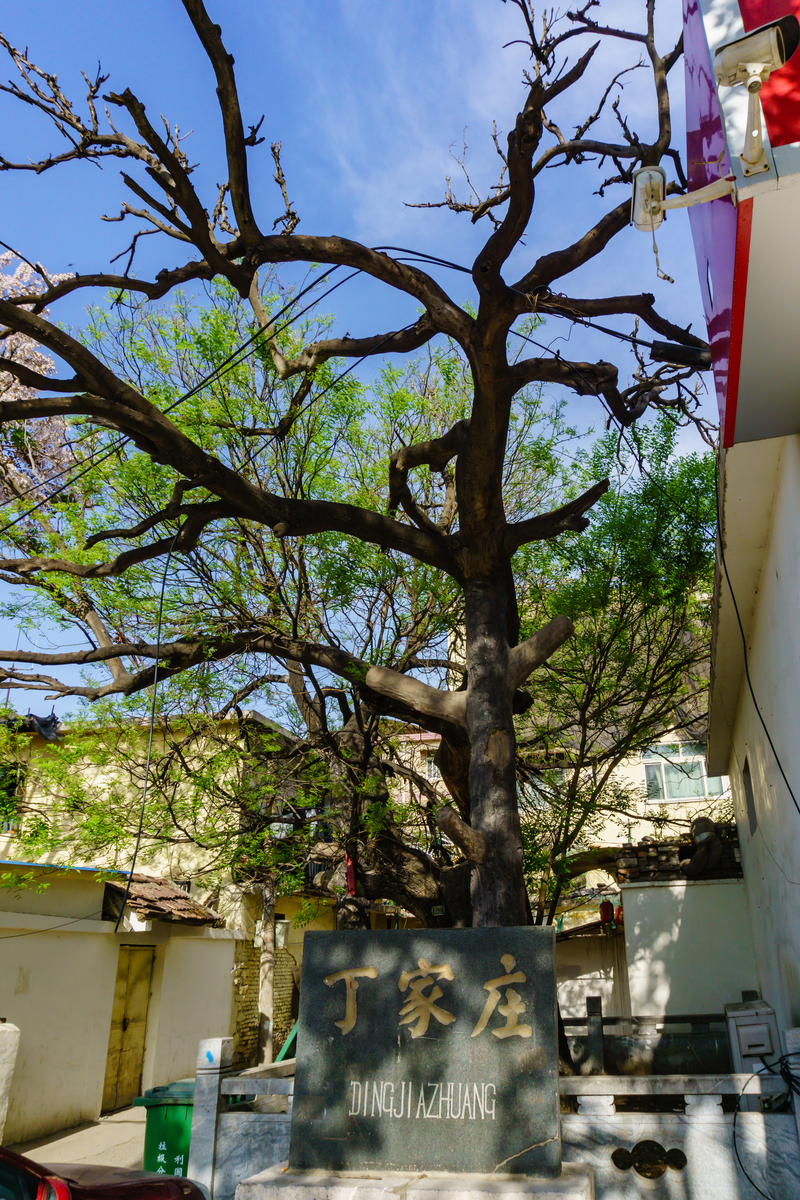
\includegraphics[keepaspectratio, height = 0.6\textheight]{dingjia/cunbei.jpg}
  \caption{丁家庄村碑}
  \label{fig:cunbei} % \raggedright \raggedright \small 2017年4月20日,丁家庄村口的村碑和百年老槐树。
\end{figure}
\clearpage


\dingphotoh{sanbadaji}{熙熙攘攘的三八大集}{2017年5月8日,丁家庄每逢农历三、八为大集。}{zuwu1}{北侧一处出租楼房外景}{2017年4月7日}

\dingphotov{guodao1}{一条街道}{2017年4月7日。}

\dingphotoh{guzhai}{城中村最为破败的一间自搭棚户}{2017年5月6日}{bizhezuwu}{笔
  者田野调查中租住的单间}{2017年4月25日,月租金240元,网络费30元,居住条件在
  城中村属于中等偏上。}

\dingphotov{chucangshi}{夫妻二人和他们一岁孩子所租住的储藏室}{2017年4月15日}

\dingphotov{cesuo1}{城中村中等水平的简易卫生间}{2017年3月31日,这类卫生间多为
  房东所建,常常加锁,只供其名下租客使用。}

\dingphotoh{yangguang}{阳光}{2017年4月26日,木制挂锁卫生间。}{lou1}{二楼房顶
  私搭简易板房}{2016年11月20日}

\dingphotov{shaoshui}{丁家庄村民常用的木柴铁皮桶炉}{2017年5月8日,丁家庄一些
  村民为节俭持家常用这种简易炉烧开水,火力弱,耗时长、烟雾较大。}

\dingphotoh{youeryuan}{幼儿园外墙与线缆}{2017年3月31日。}{wanshua}{玩耍的孩子
  们}{拍摄于2017年5月7日。}

\dingphotov{jiagai}{改造楼梯、层层加盖的一座楼房}{拍摄于2017年5月11日}

\dingphotoh{jiejing2}{街景}{2017年3月26日}{caishichang}{丁家庄综合市场中的一
  处菜摊}{2017年4月26日,年租金近9万,年耗塑料袋1万元左右。虽然是大棚内的开放
  式摊位,租金比综合市场中的活动板房小吃店还要高不少。}

\dingphotoh{caitandajie1}{城中村内一处简易搭建的菜摊}{2016年12月14日,城中村
  内一处菜摊,这里并无租金。内有被褥,卖菜大姐应当也睡在这里。}
{caitandajie2}{简易菜摊消失了}{2017年3月8日,许是抵不住严寒和微薄收入,卖菜大
  姐和她的摊位不见了,只有床垫。}

\dingphotoh{zhian}{墙上张贴的治安告示}{2017年3月31日。这里盗窃案件可能略高于
  济南市其他小区,但远未达到恶劣的程度。笔者数十次进出丁家庄,未曾见过街头吵
  架斗殴。}{diushi}{一位走丢的小孩暂在三轮车摊主的怀抱中睡着}{拍摄
  于2016年11月09日,小孩从综合市场误入城中村,寻不见家长大哭不止,后在三轮车
  饮食摊主怀中睡着,身上披着他人提供的大衣。}

\dingphotoh{hua1}{一处住户外侧的绿植与杂物}{2017年4月12日。}{yangtai}{一处阳台——花与衣}{2017年4月12日。}

\dingphotov{cbd}{丁家庄工业南路南区一户未拆住房的外墙}{2017年4月20日,丁家庄南区是第一批拆除的宅基地住房,当时已达成动迁20余户,只余3户尚未动迁。}

\pagestyle{fancy}
\chapter{城中村的简单概念}

所谓城中村者,城市和村居性质兼而有之:它往往位于城市中心或郊区,作为城市的一
部分,周边均具城市特征,自身却充斥着农村式的无序和自然,缺乏人工的总体规划,
各家各户的宅地界限比传统村庄混乱得多,基础设施(能源、通讯、供水、交通、安全、
卫生、医疗、文化等)薄弱,常住人口基本为农村户籍,土地制度仍为农村集体所有制
而非城市的全民所有制;作为农村,它的外来流动人口数量数倍,甚至数十倍于常住人
口,耕地被大量或完全占用,转为实质上的商业或住宅地产,耕地的这种性质转变使常
住人口原赖以生存的农业收入转为地产收入,并成为其收入的重要来源。

联合国对\textbf{贫民窟}的定义是“以低标准和贫穷为基本特征之高密度人口聚居
区”,对\textbf{贫民窟家庭}所作的定义为:
\begin{quotation}
  贫民窟家庭是指有以下一项或多项问题的家庭:(a)缺乏改善的饮水;(b) 缺乏改善的
  卫生设施;(c) 缺乏足够居住面积,过于拥挤;(d) 住宅的结构耐久
  性差;(e) 缺乏土地所有权的保障。
\end{quotation}

我们通常所说的城中村可以认为是中国政府棚改文件中定义的“城市棚户区”,并且明
显属于联合国定义的城市贫民窟范畴。\cite{unandchina}


中国的城市贫民窟人口有多少呢?联合国人居署提供的往年数据如下:
% Please add the following required packages to your document preamble: % \usepackage{booktabs}
\begin{table}[!ht] \centering
  \adjustbox{width=\linewidth}{%
    \begin{tabular}{l|l l l l l l}
      \toprule
      & 1990年 & 1995年 & 2000年 & 2005年 & 2010年 & 2014年 \\ \midrule
      城市中贫民窟人口的比例(\%) & 43.6 & 40.5 & 37.3 & 32.9 & 29.1 & 25.2 \\
      城市贫民窟人口的数量 & 1.316亿 & 1.514亿 & 1.691亿 & 1,835亿 & 1.806亿 & 1.911亿 \\ \bottomrule
    \end{tabular}%
  }
  \caption{1990-2014年中国城市贫民窟人口比例及数量}
  \capsource{联合国人居署旗舰报告《World Cites Report 2016》\cite{9789211327083}}
\end{table}

根据《国家新型城镇化规划(2014-2020年)》,我国预计“到2020年基本完成城市棚
户区改造任务”。根据2018年第十三届全国人大一次会议政府报
告\footnote{\url{http://www.gov.cn/gongbao/content/2018/content_5286356.htm}},
“棚户区住房改造2600多万套,农村危房改造1700多万户,上亿人喜迁新居”。全国
轰轰烈烈兴起的城中村改造跑步前进,新型城镇化取得了惊人成绩,这同时也标志着
曾经遍布每个大中型城市的老式城中村的大量消亡,丁家庄城中村也在其中。先
让我们看下曾经的丁家庄是什么样子吧。

\chapter{济南市丁家庄城中村见闻散记}

\section{背景介绍}

济南市丁家庄,又名丁家村、丁家新村,据1992年5月1日所立村碑记载:
\begin{quotation}
  明永乐年间(1403-1424)当地根据传说取村名“定妖庄”。后因此名不雅,故
  以“定”字谐音“丁”字改为丁家庄。
\end{quotation}

丁家庄隶属于山东省济南市姚家街道,曾是济南市一个较大且密集的城中村,
在2000年前就已开始为外来务工人员提供住房餐饮等生活服务,共有村民宅基地(院落)
近800户5000人,外来流动人口峰值大约可达30000人。丁家村城中改造是山东省棚改
旧改的重点项目,于2017年年底基本完成房屋拆除工作,拆迁面积约为53万平方米,
包括村民宅基地、公益性公共设施用地和经营性用地等,整体搬迁至奥体西路新建高
层小区。

\section{初见}

笔者初入丁家庄时便因它表面的破败和杂乱而产生一种恐惧感。整个城中村除20余栋6层
楼房以外,基本全是村民自建、层层加盖的三四层楼房,有的自建房已有些轻微倾斜,
有的在房顶上再加装简易活动板房;各种样式的电线、网线、不明用途的线缆随意聚成
一团团,与敞盖或无盖的配电箱、歪七扭八的电线杆纠结交织,这里似乎随时会演变为
危房倒塌或大型火灾现场。笔者倒是未闻未见相关事故,或许是因户主和租户有一套自
发自治管理的办法。

条条未经规划和硬化的水泥石板路路面也是蜿蜒曲折,纵横交错整个村落,笔者游历丁
家庄数次之后才可不迷路。出租房基本都是单间,十几二十几户共用户主搭建的公共厕
所,楼上住户冬天起夜时还要穿衣下楼,并不方便。村民们多是传统农民打扮,外来务
工人员衣着也称不上光鲜亮丽。过往中国农村生活条件艰苦,重病患者、残障、丧失劳
动能力的比例往往大于城市,而丁家庄这里的比例可能比传统农村还要高。笔者有次刚
要走出丁家庄时碰见村口一位50岁左右的男子坐在轮椅上斜着头,面无表情、眼神空洞,
对周围不管不问地在晒太阳,或许是偏瘫。未过几秒,迎面又走来一个怯生生的30岁左
右的男子。他提着午饭低头走来,看见我时便将整个身子直接旋转180度,定在原地背向
我,不敢和我有一瞥眼的接触。当我正要和他擦肩而过时,这位男子又朝无人那侧180度
急速转身,继续前行,他应有视线恐惧症或社交恐惧症等精神疾病吧。不过有路过的村
民向他热情问候。\improve{缺乏对居住人口的描写}

未接触过城中村的人,初入丁家庄,很难不恐惧吧,毕竟这里像是随时随地会发生刑
事案件一样。然而,这确实多虑了。房东们多会查看并登记租户身份信息,考察租户
人品性格,周边人群间的关系也比高楼大厦上来得亲密一些。一只只小小的、防君子
不防小人的普通挂锁足以保证财物安全。不知怎的,当我在那不足10平的单间里住宿
时,却比在现代小区高楼上居住更加平静和坦然一些。

\section{黑夜与清晨}

丁家庄城中村的夜总比周边来的更早些。

街道路灯不多,住户多使用散发着黄色光晕的白炽灯。晚上八九点钟,灯光和墙面组成
的黄色主色调混合着个别店铺的七彩霓虹灯光闪耀在城中村里,叮叮当当的做饭声时常
在周边响起,笔者还见过住处一楼楼廊里一位不足10岁的小男孩独立炒菜做饭,归来的
叔叔阿姨们在路过时对他不吝赞叹。

深夜,村外尚有较晚收摊的小吃车、大排档、夏天24小时营业的烧烤店、为深夜食客
们服务的小零售店、长明的路灯和过往的车辆。村里却是另一片景象,这里更黑更静。
晚10点左右还能偶尔听见晚归人家的锅碗瓢盆交响曲,11点左右整个村子便一下子寂
静起来,水泥石板路上鲜有路人。偶在没有路灯照耀的环卫点,有老人在几个垃圾箱
中翻找可再利用的杂物。

这里的早晨也比周边来的更早些,6、7点钟各处雄鸡打鸣,各家各样的声音均透过不
隔音的墙壁和窗户传到家家户户,问候声、寒暄声也此起彼伏。孩子、送孩子上学的
家长、上班族一下子散布各处,城中村在这个时间已经开始繁忙起来。

\section{医疗保健和社会保障}

因笔者能力有限、怠惰和调查时间选择上的问题,被调查人群多为中老年人并且数量
很少。虽然存在这种样本偏差导致不能推导出一般性的结论,但笔者认为可以提下自
己直观经验感受:不管是流动人口还是常住人口,他们身高较之周边明显偏矮,心
脑疾病比例较多,也有被调查人家庭两代人中均患重大疾病的事例。《中国心血管病报
告2017》中开篇有提“我国居民心血管病(CVD)危险因素普遍暴露,呈现在低龄化、低
收入群体中快速增长及个体聚集趋势。”,贫穷始终是种顽疾,甚至是绝症。

根据“丁家庄环境卫生管理公示牌”,丁家庄有保洁人员21人,保洁面积4万平方米。
据本次调查,济南市环保局贯彻执行八小时工作制,并为保洁人员缴纳三险。所聘用
保洁人员多为丁家庄居住人口,每月到手收入在1600元左右。济南市环保局在劳动保
障上的表现出乎笔者意料,在此点赞。另外,有一例保洁员工伤纠纷,当事人为外地
来济60多岁老人,因是否算工伤与环保局有分歧,环保局领导也曾亲切慰问。虽然当
时问题并没有解决,但当事人对国家和政府仍表示“非常满意”,没有任何意见。

丁家庄老年村民大多没有缴纳任何形式的养老保险,包括新型农村社会养老保险(新
农保),也不了解具体政策。满60岁老人由村委每月补助600元左右。丁家庄大部份村
民所能缴纳的社保只有新型农村合作医疗(新农合),有每年缴纳100元和300元两个
档次。新农合在丁家庄村民重大疾病治疗上发挥了极其重要和显著的作用,常可报
销60\% 多的费用。

\section{何不食肉糜}

虽然丁家庄北侧就是一个较大的综合市场,供周边几个社区的居民采购农副产品,生
意兴隆但年租金昂贵,大菜摊租金约9万元/年。城中村里仍有些蔬果摊子长期固定在
街道一角,它们铺设在水泥道路或机动三轮车上;还有些定期定时流动叫卖的轻型贩
菜货车。城中村蔬果摊主要面向城中村内中老年居民,无需承担任何租金,多供应次
一级的菜品并且价格低廉,但销售额和利润远不能与综合市场相比。 (可参
考\cref{fig:caishichang}, \cref{fig:caitandajie1},
\cref{fig:caitandajie2}。)

这里我们来谈一个架设在机动三轮车上的水果摊主吧,笔者将其隐去名讳,代称为刘哥
吧。即使在城中村,刘哥家的居住环境可能仍是最为糟糕的,他一家三代住在一个200多
元月租的单间中。他的立业史,也是每一步都恰被时代所驱赶和压迫的悲剧史。他做过
走街串巷流动叫卖的小贩,被驱逐淘汰;又做过居民小区外较固定的摊贩,被驱逐淘汰;
又做过丁家庄综合市场外路边摆摊的摊贩,相较综合市场的高额租金,路边摊所需费用
便宜太多,同样也是被驱逐淘汰;最后刘哥成为了城中村内一个机动三轮车上的瓜果小
贩。2017年丁家庄已被夷为平地,真正的硬汉刘哥不知又将以何种方式去往何处,拖家
带口继续书写他自己的奋斗史……

夏季的一天,笔者碰到他十岁左右的儿子从自家中捧来几片薄切的西瓜给他吃,可
他明明就是卖瓜的呀。

笔者无论如何也没有想到,当笔者向一些人说起丁家庄综合市场和城中村菜摊的区别
时,有些人会指责刘哥不努力不争气,质疑他为何不早在综合市场租摊位(高租金)
以求得良好收益。一个一家三代居住在城中村破败单间的外来人,如何去承担每年数
万的租金啊。我记得90年代初当我还是个小孩时,并没有铺天盖地地听到“成
功”“成功人士”这类说法,对于贫穷者多半是怜悯其境遇不佳。今时简单用资本结
果作为个人能力的衡量标准,从而一叶障目时,我们都将成为那个呆傻可笑的晋惠
帝,“百姓无粟米充饥,何不食肉糜?”


\section{过往的宅田基地之殇}

在中国传统小农经济的农村中,往往以家庭为基本单位,主要活动范围局限在村内,
生产集中在自家规模极为有限的耕田或从事简单手工业、半加工业的家中,生活集中
在自家住宅与村内公共空间。田区和住宅区常常分隔明显,呈大块状分布,同一大块
内常是多家彼此有联结的田地或住宅,其中相联两家之间的田地多用沟、垄、界石作
为田界,住宅之间多用共用的一面墙壁或距离极近的两面墙壁作为宅界。

多数人的社会空间长期固定、聚合、封闭在居住村,物质和社会资源有限,生产生活
单调贫乏,村民之间联系频繁,信息传播速度快,甚至可以代代相传。这种情况下发生的利益冲突常常尖
锐持久、难以调和,田界和宅界作为最重要的家庭产权,具有相当刚性。

在实践和具体的社会空间中,这一刚性界限却又常常变动并受到侵蚀。它本身包含农
村中通风、采光、日照、排水、通道等难以界定的方面,另外在国家和政府层面来说,
又有历史遗留、立法不健全、执法成本高等问题;在村民来说,则有历史遗留、普遍
违规超额占用、法律维权成本高、法制观念不强、宗族势力等问题。

如果氏族大家庭或直系小家庭被其他大小家庭侵犯界限而未采取有效措施,则不单是
家庭经济效益,连带个人和家庭的自我认同、社会地位也将受到严重负面影响。这
也使宅、田基地矛盾相当尖锐频发,家庭中的强壮男子往往被赋予保卫甚至扩张这一
刚性界限的责任。过往中国对家庭伦理的重视,甚至重男轻女等现象,也多由此建立
起来。

在笔者对丁家庄的走访过程中,也曾碰到宅基地纠纷当事人商姐(化名)说起一例二十多年前
的惨剧:两家因新修墙壁越界而产生的宅基地矛盾步步升级,致使受到屈辱的商姐丈
夫自杀。商姐带领家人将邻居群殴至半死,法院支持了邻居的索赔诉求,但商家一家
并未履行法院判决,于是被打邻居二十余年不允许商姐家开发自家一块空地。

丈夫自杀后,商姐带着两个儿子独立生活,其中小儿子当年不到两岁。她抓住了空间
转化的时机,是90年代丁家庄第一批建立租屋的人。丁家庄拆迁前她的租屋总面积已
经超过1500余平,出租房屋超过50户,月入过万,在丁家庄这也是了不起的成就。她
的两个儿子也争气,可给她带去一些宽慰,只是长年的劳苦使其腿疾明显,面态老相,
但商姐勤劳不改,晚上仍会去丁家庄综合市场进行清洁工作,以换取一些额外的微薄
报酬。总是风风火火、穿着男式西装、一瘸一拐地支撑起整个家庭的商姐啊……

当商姐以维权为理由向我极为悲愤倾诉她的故事时,笔者一再说明我这个自发小项目不能给其带来
任何改变,也难以根据她的一家之言去支持她时,她对笔者的中立态度表示认可,最
后甚至还埋怨起她的家庭当年为什么不让一下那寸土的界限,即使再让更多些也不要
紧啊……

诉说过程中,笔者渐感商姐并非真要维权,并非还存那样的恨意。她曾说要带笔者去看
那块因久被搁置而自然成为停车场的空地,笔者当时就感觉可能此事到此为止,事实上
也是如此。事后我为求证自己想法两三次询问时间安排时,她果然都借故推脱,并
刻意回避我。

她真正想要的其实只不过是一场没有利害关系的倾诉……倾诉完之后当事人产生了羞
愧感,不敢面对被倾诉人;而所谓仇恨早已经在时空的变换中变成了一大块难看疮疤。

随着丁家庄旧村改造的完成,丁家庄人将进入新的、现代化的城市空间,城市空间中
的界限更为明显也易维权,原本农村中典型的宅基地矛盾将很少存在,希望两家日
后能够相忘于江湖,也同样希望人们彼此能够多一些理解,多给一些倾诉的空间,以
使悲剧不再那么多,那么难以令人承受……



% 丁家庄城中村是一个充斥着盎然生机、孕育着诸多可能的城中村。它是许多人实现梦想的起% 步点或中转站,也展开怀抱接纳了各方边缘人群,诸多住户之间较为和谐。它也远未成为一% 个堕落之处,这里并非治安恶化严重,


% \section{失败的丁家庄城中村社会学调查}

% 笔者起初准备以定量研究方法结合定性研究方法对丁家庄作一个较为全面的社会调查。其中定量方面,仿照ISSP\footnote{The International Social Survey Programme,国际社会调查方案}和中国的CGSS\footnote{Chinese General Social Survey,中国综合社会调查,于2007年加入ISSP。}问卷作一个针对丁家庄城中村的调查问卷,定性研究初步决定采用Phil Francis Carspecken的批判定性研究框架。

% 之后笔者又十几次进入丁家庄,也曾在丁家庄居住做过1个月进行田野调查,但因自身怠惰和三心二意使本次调查大失败,不过以下几点心得或许有益于类似社会调查的开展,在此分享给读者:
% \begin{enumerate}

% \item 定性研究一般要求记录谈话,录音常是记录谈话的主要方式。扎根理论和Carspecken的定性框架必须建立在大量谈话资料的多次整理上。但丁家庄人均谈录音色变,拒绝录音。这种拒绝主因是被调查人在敏感性的事件上害怕录音成为某种对自己不利的证据。

% \item 城中村人员组成和住房结构的复杂,使针对整体的概率抽样问卷调查非常困难。实际上笔者认为,只有具有政府背景的组织或机构大力支持、推动才能完成类似复杂区域定量研究的概率抽样。

% \item 笔者采用了非概率的随机街头访问方式发放调查问卷,这使调查结果可能产生无效的、完全不具代表性的样本。并且即使如此,问卷回收率仍然极低,只能勉强算是10\%,使定量分析成为不可能。

% \item 利益敏感问题信度不高。除笔者本人能力拙劣外,也有现实客观。例如针对房东的调查中,房东往往隐瞒和减少实际出租房屋间数以及出租收入,可从被调查房东所处房子建筑外观、体积以及丁家庄出租房的平均面积和收入得出这一信度不高的结论;针对所有人的收入问题也存信度问题,再三询问或试探所得出的收入结论最高浮动为1000多元人民币。调查问卷中针对村委和拆迁方案的满意程度采用了5级李克特量表,但被调查人极端选择较多,情绪化明显,个人利益最大化主导的倾向明显。

% \item 半数以上房东有对上级政府机构的强烈诉求,这也是他们对社会调查人最大的期望。本次调查为笔者个人自发,没有任何组织机构背景,也一再向被调查人言明本人所写报告预计不会产生任何一点社会影响力,无法满足房东这种诉求。除此之外,社会学可以采取小额金钱奖励的方式来增加被调查人积极性,但笔者着实囊中羞涩,无法采用这种方式。

% \item 租房人对本次社会调查表现出严重的整体冷漠,可以认为这是一种社会排斥。关于这方面内容,笔者放在之后章节再详细论述。小额金钱奖励应可以有效提高租房人积极性,但未实施,原因同上。

% \item 最主要原因仍是笔者个人社会调查能力的欠缺,和态度的不端正。笔者接触社会学是在丁家庄摄影项目受阻之后从零开始,在社会学意义上的与人交往也存各种缺陷。最主要的还是态度,三心二意、半途而废,甚至因屡次消沉而遗失了几份已经回收的完整调查问卷。

% \end{enumerate}

% 本次调查过程中,笔者听闻有两位女士几乎同期在丁家庄城中村进行社会问卷调查,并对问卷完成者提供每人50元奖励,效果不错。笔者估计是具有政府背景的组织机构,如大学在做这份工作。希望我国能够在当前基础上进一步普及社会学调查相关知识,增加社会学调查项目,并保证社会学调查的中立性及公信度,同时也希望调查者能够坚守信度和效度问题。


\chapter{希望的与绝望的贫民窟}

碍于笔者懒惰,未再追踪奥体西路丁家庄回迁安置区的情况。但对于本书立意来说,其
实也无多少必要去追踪………

% 中外城中村对比。

% 空间生产、新型城镇化 2000年。

\section{希望的贫民窟与绝望的贫民窟}
\label{sec:hopedespair}

中国的城中村早先多是位于中大型城市郊区的传统农业村庄;上世纪90年代农村向城市、
小城市向大城市、中西部地区向东部地区劳动力大规模流动转移的“民工潮”,使城中
村始现;随着21世纪初人口流动逐渐全部放开、工业化和城市化进程加快,城中村
开始兴盛,成为城市景观中一个特殊部分。

在此过程中,城中村原常住民集体农地逐步减少,多转为事实上的集体工商业出租用地;其
中一些村集体也由此走向富裕之路;村民主要收入由农业转为出租,非规划占地、无序
自建房屋;城中村也由此成为不断扩张的城市的一部分;城中村基础和配套设施薄弱,
且仍保留着部分乡村特色;常常薄薄一墙之隔,里边是城中村,外边是摩天大楼和现代
化道路。

当一群群、一波波外来务工人员们背井离乡来到城市时,城中村给了他们一个暂时的落
脚地,提供最基础生活保障,使他们得以省吃俭用、向着梦想奋斗,在此过程中,不少
人创造了一个个发家致富的奇迹,也为一些赤贫、生理或精神病患者提供了一个并不足
以保暖御寒的家园。

联合国2003年发布了《贫民窟的挑战》报告,报告描述了两种贫民窟——希望的贫民窟
和绝望的贫民窟。

笔者认为大可不必多提一些量化分区指标,以准确补强定义,那是专家干的事情。我们
可以依托世俗对“希望”和“绝望”两词的理解,对联合国定义补充如下(粗体为笔者
自加注释):
\begin{description}
\item[希望的贫民窟] “进步”的住区,其特点是新的、通常是自建的建筑,通常是非法的
  (例如擅自占地)。这些建筑正处于或最近经历了发展、巩固和改善的过程。\textbf{大部
    分住民的生活质量有基本保障或逐步提高;存在阶层跨越空间,部分人得以搬离贫
    民窟,住进其他拥有完善配套设施和产权的现代化社区。}
\item[绝望的贫民窟] “衰落”的住区,其环境条件和配套服务正在经历退化的过程。\textbf{大
    部分住民对未来丧失信心,人文环境恶劣,难以阶层跨越,多发违规违法事件且难
    以根治。}
\end{description}

中国几乎全部城中村都为丁家庄类似“希望的贫民窟”、并且绝大部分城中村也已改造
完成,不少原常住人口、产权人也已住上现代化高楼大厦,配套设施较为完善,彻底脱
离“农村”,正式成为“城市”的一分子。甚至世界的贫困状况也主要因中国一系列扶
贫安置政策而得以明显改善,联合国多次对中国不吝赞美之辞。

“绝望的贫民窟”在中国极少,但也有,如曾经的深圳龙华三和人才市场周边,“三和
大神”们“干一天,玩三天”,身份证等个人信息材料多抵卖给违法犯罪团伙,负债累
累,挂逼\footnote{三和群体的象征性概念,常指遇到了特别困难的情况,比如身无分文,有时
  也指身亡。但大多时候指的是基本上身无分文又无事可做的状态。进入“挂逼”状态
  时在三和所能买到的最廉价的商品则被称为“挂逼×”,如人民币五元一碗的“挂逼
  面”(清汤面),五角一支的“挂逼烟”(“红双喜”牌),两元两升的“挂逼
  水”(也叫“大水”,一般为“清蓝”牌),十五元一晚的“挂逼床位”等。}习以
为常……


当城市化、工业化加速发展之时,很多城中村被列入市政规划。一些城中村居民希望借
此获得更多收益,住上一至多套宽敞明亮新房,政府也为其配备了集体工业用地、商业
用房用以补偿村集体经济。


但是也有一些家境更为贫寒、缺乏可持续收入来源的居民确实不希望搬迁,因为搬迁进
入高层楼房意味着相对高的生活成本,同时失去了原有稳定的房租收入来源。而外来租户的
权利,更是往往被忽视,因其“大可去其他地方出租”,似乎很“公平”。前文中的瓜
果商刘哥和曾经居住在此的边缘人群又将去经历怎样的风雨,去怎样奋斗呢?在恩格斯、
列斐伏尔、哈维等关于空间生产、城市权利的论述中,有条可怕的论断:现代社会城市
更新的过程亦是阶级再生产的过程;在旧的差的空间被“建设性摧毁”,城市边缘人被
抛离出原住所后,更旧的更差的空间必将在他处生产出来。

这意味着希望的贫民窟将向绝望的贫民窟步进转化……


% 另外,快速城市化、工业化的进程必然面临着一个越来越尖锐的矛盾:个别“钉子
% 户”为维护自身利益最大化漫天要价,会对整体规划产生巨大损耗,甚至导致规划夭折。
% 这是新自由主义所宣扬的市场和个人功利的必然结果。为应对这种局面,资本将可能联
% 合政府使用强制手段去摧毁这部分群体的个人功利。当资本的大自由去吞噬部分人
% 的自由,也在损害自由主义所宣扬的法理……

% \chapter{马克思主义视角的空间生产摘抄}

\section{恩格斯 《论住宅问题》}

臧峰宇《恩格斯〈论住宅问题〉研究读本》:
\begin{quotation}
  我所说的“欧斯曼计划”,是指把工人区,特别是把我国大城市中心的工人区从中豁
  开的那种已经普遍实行起来的办法,而不论这是为了公共卫生或美化,还是由于市中
  心需要大商场,或是由于敷设铁路、修建街道等交通的需要。不论起因如何不同,结
  果到处总是一样:\textbf{最不成样子的小街小巷没有了,资产阶级就因为这种巨大成功而
    大肆自我吹嘘,但是,这种小街小巷立刻又在别处,并且往往就在紧邻的地方出
    现。}\pagescite[][243]{maenwen3}

  住房短缺也是这样。现代大城市的扩展,使城内某些地区特别是市中心的地皮价值人
  为地、往往是大幅度地提高起来。原先建筑在这些地皮上的房屋,不但没有这样提高
  价值,反而降低了价值,\textbf{因为这种房屋同改变了的环境已经不相称;它们被拆除,改
  建成别的房屋。}市中心的工人住房首先就遇到这种情形,因为这些住房的房租,甚至
  在住户挤得极满的时候,也决不能超出或者最多也只能极缓慢地超出一定的最高额。
  这些住房被拆除,在原地兴建商店、货栈或公共建筑物。波拿巴政权曾通过欧斯曼在
  巴黎利用这种趋势来大肆敲诈勒索,大发横财。但是欧斯曼的幽灵也曾漫步伦敦、曼
  彻斯特和利物浦,而且在柏林和维也纳似乎也感到亲切如家乡。结果工人从市中心被
  排挤到市郊;工人住房以及一般较小的住房都变得又少又贵,而且往往根本找不到,
  因为在这种情形下,建造昂贵住房为建筑业提供了更有利得多的投机场所,而建造工
  人住房只是一种例外。\pagescite[][193]{maenwen3}

  在当今的时代条件下,我们发现恩格斯对住宅问题的分析也具有某种空间权利及空间
  正义的考量。他对资本统治下城市空间的分化隔离、无产阶级和小资产阶级生存空间
  被剥夺的现象进行了科学分析,把城市空间的矛盾归结为资本主义生产方式本身,实
  乃深刻的思想洞察。\pagescite[][74]{zhuzhaiwenti}

  我们可以从以下两个层面来理解资本逻辑的特征:\textbf{其一,资本逻辑是以资本的增殖
    为终极目的而把一切变成为实现这一目的之手段的一种强制关系。}在这一关系中,
  资本增殖是一切行动所围绕旋转的轴心,而作为创造资本的主体--劳动者却被降低为
  被剥削的对象和役使工具,其创造的剩余价值被资本家无偿占有。\textbf{其二,资本逻辑
    的展开过程就是资本逻辑内在矛盾形成和发展的过程。}资本逻辑的过度膨胀造成了
  无产阶级的极端贫困,激化了社会矛盾,产生了诸多社会问题以至于威胁到资本的统
  治,从而迫使它寻求维系剥削与总体利润最大化的长远机制,其外在表现就是资产阶
  级解决社会问题的种种尝试,这在一定程度上反映出资本主义制度自我修复、自我进
  化的能力。当然,这只是资本逻辑的自我循环。

  资本拜物教的信徒对于社会问题的认识必然基于对资本逻辑的认同,他们从不怀疑这
  一逻辑本身……这也就决定了资产阶级在看待社会问题上的局限
  性。\pagescite[][100]{zhuzhaiwenti}

  房租的背后是资本的生产链条以及经济规律的调节作用。其中主要的一环就是地租,
  这是由于城市的迅速发展使得现实的经济条件发生了重大变化,\textbf{因为工业和商业资本
  的有机构成高于农业,所以为了加快资本周转和创造剩余价值,就必须让渡给土地所
  有者更多的地租,以便于城市土地顺畅地参与市场资源的配置。}
\end{quotation}

\section{列斐伏尔}

张笑夷《列斐伏尔空间批判理论研究》:
\begin{quotation}
  \textbf{空间的生产不是资本主义生产方式自然而然的再生产,而是被构想的和深思熟虑的
    结果。空间具有政治性,它是政治统治的工具,空间的生产是现代主义国家的政治
    战略。}“空间与政治国家的关联比曾经的领土与民族国家的关联更牢固。它不仅被
  生产力、生产关系和所有权生产;而且它是一种\textbf{政治产品},具有行政和残暴统治性
  的产品、由政治国家上层统治关系和战略决定的产品。并且,这不是在某一政治国家
  范围内,而是在国际和全球范围内,在全球国家体系范围内的生产。”

  从列斐伏尔的观点来看,资本主义生产方式生产了它自己的空间,在空间的生产的进
  程中资本主义的生产方式改变为 “\textbf{国家生产方式}”。同时,空间不仅成了生产力
  要素、生产关系和所有权关系要素,还完全成为政治性的,政治性的空间在当今资本
  主义社会中成为主导性的。空间的政治性主要表现为,首先,空间是意识形态的,它
  是社会技术专家治国制的表象。其次,空间是实践的,是政治权力的工具和手段。最
  后,空间是战略性的,它从属于政治目标,被纳入了剩余价值的生产。

  在过去资本主义的长期发展中,土地曾被视为封建地主阶级的残余而被忽视,建筑业
  的重要性曾远远不及钢铁生产、制糖工业等。而现代资本主义生产实践则相反,\textbf{土
    地进入了生产关系再生产的范畴,在新资本主义的结构性生产关系中处于中心地
    位。}显而易见,政府的住房规划就促进了这种\textbf{以 “不动产” 的动产化为特
    征}的空间的生产。住房建筑与土地不可分割,土地构成住房价值的一部分,于是,
  被分割的一块一块土地成了空间性的产品。“因而,资本投资在房地产部门中找到了
  一个避难所,一个补充性和互补性的剥削领域。......在一些国家中,比如西班牙和
  希腊,房地产部门已经成为由相当熟悉的政府干预形式所构成的经济的一个必不可少
  的组成部分。在其他国家,比如日本,求助于房地产部门来弥补通常的生产--消费循
  环带来的困境并增加利润,这已是稀松平常之事:甚至对房地产部门进行事先预测和
  规划。” 基于作为整体的空间的生产的新资本主义的增长战略为了实现空间的生产而
  进行的空间动员开始于土地,然后,这种动员延伸到地下空间和地上空间,从地下的
  能源、原材料资源、地面的土地资源到地上的被建筑或各种需要分隔出来的空间容量
  都被赋予了交换价值,作为整体的空间成了一个更庞大的 “商品世界”。过去我们买
  卖或租赁的是土地,而今是房屋、楼层、公寓、停车场、游泳池等各种各样的可交换
  可计量的碎片化的空间。 “\textbf{空间成为商品,把空间中的商品特征发展到了极致。}”

  列斐伏尔说: “如果我没记错的话,在 20 世纪 60 年代初,有一个关于空间战略的
  高层决策;不是欧洲的,不是欧洲的空间战略,而是一个法国的空间战略。换句话说,
  它描绘着中心化,巴黎的中心化。巴黎必须变成像鲁尔或英国的巨大都市一样的财富
  和权力的都市核心。这是关于空间政策的政治决定。”因此,\textbf{中心化需要更高的政
    治理性,也就是需要国家或者叫作都市理性以更有效的方式,也就是在全球范围和
    整体上生产空间,通过这种空间秩序的中心性驱逐边缘要素,强有力地集中财富、
    行为手段、知识、信息和文化。同时,因为中心化是一种政治决定,它还需要技术
    和知识的代理人,也就是规划者为中心化提供不证自明的合理性。}

  工业化带来的破坏——史无前例的大规模地重建,即\textbf{在整个社会的规模上进行重
    建。} 这一过程的推进,伴随着许多越来越深刻的矛盾。现存的生产关系被推广、
  扩张了;在同时把农业和都市的存在整合起来的过程中,它们又带来了一些新的矛盾:一
  方面,\textbf{拥有某些未知的权力的决策中心}已经形成,因为这些中心集中了财富、压迫
  性的权力和信息;另一方面,对过去的城邑的破坏,使得各种形式的隔离成为可能,
  各种社会力量无情地将人们\textbf{在空间中分隔开来}。由此,一种广泛意义上的社会关系
  解体了,而与之相伴随的,则是和所有制关系密切相关的那些关系,被集中化
  了。”总体来说,资本主义国家和政治权力主持整合历史城市和农业,把地下、地面
  和地上的空间以及世界范围的空间作为整体进行规划,为寻求日益稀缺的能源、水、
  光等资源而被重组。\textbf{在这个过程中形成的都市空间既是统一的又是分离的,都市空
    间被分割和分隔成彼此分离又相互叠加的异常复杂的空间碎片,国家和政治权力保
    证碎片化的都市空间相互联系,同时,国家和政治权力正是通过历史城市的碎片化
    和中心化建构来保证都市空间的统一性。}

  当国家和政治权力占据它所生产的空间时,日常成了政治建筑屹立其上的土壤。权力
  处心积虑地联合技术和实证知识,小心翼翼地维持着日常生活的连续性,把都市社会
  伪装成具有虚假透明性的 “抽象空间”,结果是,这层神秘的面纱把都市社会的日常
  生活笼罩在恐怖主义之中, “\textbf{对社会成员来讲,到处弥漫着恐怖,暗藏着暴力,压力
    来自四面八方,只能通过超人的努力来避免或转移这种压迫;每个成员都是恐怖分子,
    因为他们都想掌权;因此,无须有一个独裁者;每个成员都自我背叛和自我惩罚;恐怖不
    能被定位,因为它来自四面八方,来自每一件事; ‘系统’ (如果能被称为 ‘系统’
    的话)掌控着每个单独的成员,并使每个成员服从整体,也就是,服从一个战略,一个
    隐藏的结局,这些目标除了掌权者外无人知晓,也无人质疑。}”

  在法国就存在着一个过于庞大的中心,这就是法国的首都巴黎。巴黎作为决策和舆论
  中心统治、剥削着分布在巴黎周围的从属性和被等级化的空间,从而在法国内部建立
  起了一种\textbf{新殖民主义},形成了\textbf{“超发达、超工业化、超都市化的地区” 与欠发达和
    贫困状况日益加剧地区的不平衡发展的矛盾}。同时,他也指出,在现代世界
  里,\textbf{“边缘” 具有多重含义}。首先,边缘在广义上包括资本主义生产方式下被剥夺生
  产工具的\textbf{世界无产阶级}。狭义上来讲包括世界范围内的不发达国家特别是\textbf{前殖民地
  国家}。其次,在资本主义国家内部,边缘指那些\textbf{远离中心的区域}。比如,法国的布
  列塔尼,大不列颠的爱尔兰、威尔士和苏格兰,意大利的西西里岛和南部地区等。再
  次,边缘指\textbf{城市的边缘地区、城郊的居民等}。最后,边缘还指那些\textbf{社会和政治的
    边缘群体},特别是青年和妇女、同性恋者、绝望的人、“精神错乱” 的人、吸毒
  者等。中心和边缘的矛盾不仅仅表现为单方面的中心对边缘的控制和剥削,以及中心
  和边缘发展不平衡的加剧。

  同化和同质化的过程必然伴随着激烈的反抗,中心越倾全力控制和剥削边缘,边缘对
  中心的反抗和违反就越激烈,中心越连续和无限地控制和剥削边缘,边缘对中心的反
  抗和违反就越持久和永恒。另一方面,\textbf{国家资本主义和国家把城市作为财富、决策、
  信息和空间组织的中心,伴随着中心的饱和、资源的匮乏等问题的出现,城市发展逐
  渐显现出衰退迹象,从而使中心化危机显露出来并不断扩展,甚至恶化。}美国的都市
  化进程最迅猛,相应的城市问题和城市危机也最先暴露出来。“\textbf{美国资本主义曾经面
  临极度痛苦的两难境地:是应该牺牲城市(纽约、芝加哥、洛杉矶等)并在别处组建决策
  中心(这是件很难的事) ,还是应该通过投入巨大的资源来保留这些城市,即使是美国
  社会自己所能支配的资源的总和也在所不惜。}”

  总之,国家资本主义的都市化进程生产了中心、边缘及其矛盾,\textbf{中心的衰落和中心与
  边缘矛盾的加剧引发的城市现象和城市危机使城市成为资本主义矛盾表现最激烈的场
  所。}列斐伏尔认为,资本主义抽象的都市空间中质与量的矛盾、交换价值与使用价值
  的矛盾、为非生产性消费和生产性消费进行的空间的生产之间的矛盾、暂时与稳定的
  矛盾、都市理性统治下抽象空间的意识形态化等矛盾是中心和边缘矛盾的征兆,同时
  也是其原因和结果。
\end{quotation}

\section{大卫·哈维}

大卫·哈维《叛逆的城市》\cite{harvey2012rebel}:

\begin{quotation}
  资本家资本主义永远都在生产城市化所要求的剩余产品。反之,资本主义也需要城市
  化(与此相关的还有其他一些现象,例如\textbf{军事开支}等等)来吸收无止境生产出来的
  剩余产品(\textbf{惊险地一跃})。因此,\textbf{资本主义发展与城市化之间呈现出一种内在的
    联系。}

  \textbf{贯穿于整个资本主义历史,城市化从来都是吸收剩余资本和剩余劳动力的关键手段,
    城镇化凭借不断变更空间和场所的使用功能,实现空间垄断及垄断地租,进一步推
    动资本积累。}

  如果劳动力短缺,劳动力工资太高,那么必须重新培训现存的劳动力(以技术手段引
  起失业,或打击有组织的工人阶级力量——如撒切尔和里根在20世纪80年代所采用
  的——是两种基本方法),或者找到新的劳动力。从一般意义上讲,必须要找到新的
  生产方式;从特定意义上来讲,必须要找到新的自然资源。

  1848年的经济危机是一个明显的无法利用剩余资本和剩余劳动力的危机。拿破仑公布
  了一个宏大的海内外基础设施投资项目……最重要的是重建巴黎的城市基础设施。奥
  斯曼使用了类似\textbf{凯恩斯}\footnote{不是经济学发明经济模式,而是经济学总结发现已有的
    经济模式}的体制,利用债务融资,改善城市基础设施,从而解决剩余资本的出路问
  题。

  奥斯曼清楚地认识到,他的使命是\textbf{通过城市化来帮助解决剩余资本和失业问题}。当
  建筑师雅克·伊尼亚斯·希托夫向奥斯曼展示他关于巴黎新林荫大道的设计方案时,
  奥斯曼驳回了这个方案,他说:“不够宽……\textbf{你的设计宽度是40米,我要的
    是120米}。”他吞并了郊区,重新设计了整个街区,如Les Halles。要做到这一点,
  奥斯曼需要\textbf{新的金融机构和债务工具},即建立在圣西门基础上的\textbf{流动信贷和不动
    产信贷}。实际上,他建立了一个 \textbf{原始凯恩斯体系,利用债务融资,改善城市基
    础设施,从而解决剩余资本的出路问题。}

  在随后的15年中,这个类似凯恩斯主义的体制运行良好……\textbf{但是这种过度扩张,以
    及日益具有投机性的金融和信贷制度最终于1868年崩溃。}奥斯曼被迫下台。绝望中
  的拿破仑三世发动了与俾斯麦德国的战争,并以法国的失败而告终。

  二战后,罗伯特·摩西在整个纽约都市区再现了奥斯曼在巴黎的作为。他改变了有关
  城市发展的思维尺度,\textbf{通过(由债务融资建设的)高速公路系统和基础设施改造,
    通过郊区化,通过对城市和整个都市区域的重新建设来吸收剩余产品,进而解决剩
    余资本的吸收问题。}当上述过程在全国范围内的都市区域推行时,对战后全球资本
  主义的稳定发挥了关键作用。

  尽管郊区化在战后发挥了巨大的作用,但郊区发展是以\textbf{掏空城市中心}为代价的。聚居
  在城市中心的少数族裔因此被隔离在新的繁荣之外,并受到极大的负面影响,从而导
  致他们的反抗,进而产生了人们所说的“\textbf{城市危机}”。

  直到2008年,美国人一直认为,\textbf{住宅市场是美国经济重要的稳定器},尤其是
  在20世纪90年代末高技术崩盘之后。通过新的建设,房地产市场直接吸收了大量剩余
  资本,而在历史性的低利率条件下,抵押贷款再融资的浪潮导致了住宅资产价格急剧
  飞涨,从而推动了美国国内消费品市场和服务市场。美国用平均日借款20亿美元来维
  系其不可满足的消费,同时以借贷融资开展阿富汗和伊拉克战争。

  \textbf{全球性城市化的繁荣一直依赖于建立新的金融体制和措施,以便组织起维持城市化
    的信贷需要。}开始于20世纪80年代的金融创新,特别是销售给世界范围投资者
  的\textbf{地方抵押贷款的证券化和打包},建立\textbf{持有债务抵押债券的新型金融机构},都
  发挥了关键的作用……它分散了风险,允许\textbf{剩余储备更容易地介入过剩的住房需求}。
  通过金融机构间的协调,这类金融创新导致\textbf{整体利率下降(给那些创造奇迹的金融
    中介机构带来了巨大的财富)}……但是,分散风险并不等于消除风险。而且,由于
  风险可以转嫁到其他地方,这样广泛的风险分散甚至鼓励了\textbf{更加风险的地方行为}。
  由于\textbf{没有适当的风险评估管理},抵押贷款市场已经失控……财政亏空,都再次呈现
  在2008年的次贷和住宅资产危机之中。

  地方政府债务的急剧上升和对投资公司借贷控制不力(多由政府主导)现在被认为是
  中国经济的主要风险,不仅给中国也给全世界的增长前景蒙上了深深阴影。截
  至 2011 年,中国政府估计市政债务约为2.2万亿美元,相当于“全国国内生产总值的
  近三分之一”,其中 80\% 的债务可能由地方政府融资平台公司持有,这些公司由市
  政府主导,但严格来说不是市政府的一部分。这些组织正在以极快的速度建设新的基
  础设施和标志性建筑,使中国城市如此壮观。但\textbf{市政当局的累积债务是巨大的。一
    波违约浪潮“可能成为中央政府的巨大负债,中央政府背负着约2万亿美元的债
    务:”崩溃之后是长期“日本式停滞”的可能性是非常真实的。}2011年中国经济增
  长机器的放缓已经导致进口减少,而这反过来又将反弹到世界上所有那些在中国原材
  料市场的支持下蓬勃发展的地区。

  吸收剩余已通过“\textbf{建设性摧毁}”引起了反反复复的城市重建。由于穷人、弱势群体
  和在政治权利上被边缘化的那些人总是首当其冲且受到最严重的影响,所以城市重建
  基本上总是具有阶级性的。新的城市是在旧城市的残骸上建立起来,因而需要暴
  力。

  \textbf{几乎在世界上的每一个城市都可以看到因有钱人而产生的建设高潮——而有
    钱人通常具有类似的令人沮丧的性格。与之相伴的是农民在农业工业化和商业化中
    变得一无所有,洪水般地涌向城市,沦落为贫困的城市移民。}

  贯穿整个资本主义历史,国家通过税收拿走一部分剩余资本。在其社会民主阶段,这
  一比例显著上升,国家控制了大部分剩余。最近30年新自由主义一直向\textbf{剩余资本私
    有化}发展……其主要成就是,阻止了国家按照20世纪60年代的方式来增加税收。更
  进一步的举措是\textbf{建立新的治理体系,将国家和企业利益相结合,并且在城市改造中
    应用货币权力,确保国家机构的剩余资本支出利好于企业资本和上层阶级。}

  \textbf{在过去的几十年里,新自由主义让富裕精英的阶级力量得以复原。}
\end{quotation}




%%% Local Variables:
%%% mode: latex
%%% TeX-master: "../main"
%%% End:

% \section{土地金融}
\label{sec:92tudi}
\url{https://www.thepaper.cn/newsDetail_forward_11744994}


% 非常重要!!!!!!!!!!!!!
% !!\textbf{https://www.aisixiang.com/data/138457.html}
% \textbf{王小鲁:土地财政的昨天、今天和明天}

% https://pdf.dfcfw.com/pdf/H301_AP202305101586440193_1.pdf
% https://www.gov.cn/gzdt/2008-12/19/content_1182391.htm
% 刺破的泡沫—海南房地产往事  沈奇 杨政 https://www.sohu.com/a/761245832_482521
% 从沸腾到癫狂:泡沫背后的中国房地产真相
% 26年了,五届全国金融工作会议重大金融改革回顾(上)
% https://new.qq.com/rain/a/20231029A080O900

\subsection{海南房地产泡沫危机}
\label{subsec:hainan}


1988年8月23日,海南脱离广东省独立建省,并在海南设立经济特区。海南成为当时中国
最新、最大且是唯一的省级经济特区,成为全国各地淘金客们的狂欢
地。1989年到1993年间,商品房平均价格从1400元/平方米到7500元/平方米;商品房年
销售面积从1000万平方米到9000多万平方米;房地产投资总额从3.2亿元到93亿元;土地
价格从几十万元/亩到600万元/亩,


\begin{quotation}
  据太平洋证券数据,高峰时期,当时总人数不过656万的海岛上有两万多家房地产公司,
  平均每300个人一家房地产公司。与此同时,大量金融机构进入,海南短时间内成立
  了20家信托投资公司,35个城市信用社,此外还有一批股份制、会员制的金融性公司;
  证券行业从1989年初建立海南省证券公司,到后来已发展为26个证券机构34个证券交
  易点。\footnote{沈奇 杨政《刺破的泡沫—海南房地产往事》}
\end{quotation}
海南房地产此时玩的已经是金融“击鼓传花”游戏,下海官员、批条、虚拟概念(方案
和图纸)、信贷、炒楼花、炒地皮、炒项目,上一人传给下一人,死的是最后一个接盘
侠……

\begin{quotation}
  1993 年 6 月 23 日,时任国务院副总理的朱镕基发表讲话,宣布终止房地产公司上
  市、全面控制银行资金进入房地产业。24 日,国务院发布《关于当前经济情况和加强
  宏观调控意见》,\textbf{16 条}强力调控措施包括严格控制信贷总规模、提高存贷利率和
  国债利率、限期收回违章拆借资金、削减基建投资、清理所有在建项目等。银根全面
  紧缩,一路高歌猛进的海南房地产热顿时被釜底抽薪。这场调控的遗产,是给占全
  国 0.6%总人口的海南省留下了占全国 10%的积压商品房。全省“烂尾
  楼”高达 600 多栋、1600 多万平方米,闲置土地 18834 公顷,积压资金 800 亿元,
  仅四大国有商业银行的坏账就高达 300 亿元。
\end{quotation}

当时在海南炒房的“万通六君子”之一的潘石屹自述当时在泡沫破裂前成功抽身的原因:
\begin{quotation}
  我到海口规划局查了一下我们的项目,是有(证件)的。我这人特别好学习,除了看
  完自己的,我还要看看别的项目。

  我记得数字(海口规划局统计的海口人均住房面积)是四十九平方米。当时北京的人
  均住房面积是七点四平方米,而海南刚刚建省,在海口这样一个不富裕的地方,电都
  没有,一个红绿灯都没有的地方,建房子要接近五十平方米,北京才七平方米多。

  这就是房地产泡沫啊,跑的越早越好。于是我就赶紧跑到北京来,做了第一个项目,
  在阜成门这边,万通新世界广场,赚了不少钱。海口的企业家,多少企业家,基本上
  全军覆没,出来的很少。

  有好多人说,我们几个人,能够从海口这边逃着出来,能够从海南岛的92、93年房地
  产泡沫里逃着出来,非常聪明,很有远见。其实呢就是算数,就是建筑面积除一个人
  口数。就是常识。

  不要把这些商业的东西搞的多神秘,一会儿佛了,一会儿道了,一会儿鬼了,一会儿
  神了,没有这么神秘的东西,就是要尊重常识。
\end{quotation}
多么聪明,举一反三的潘石屹啊!你信么?反正笔者不信。


同期不止海南,北海、惠州、上海等地也出现了房地产热。朱镕基在1999年1月8日
在省部级领导干部金融研究班上对这时期的房地产热总结到:
\begin{quotation}
  从计划经济体制向社会主义市场经济体制过渡中,许多长期积累的深层次矛盾集中反
  映在金融领域。仅从房地产看,1992年、1993年的房地产热,就造成银行不良贷款几
  千亿元。目前,全国闲置的商品房多达7000多万平方米,价值在4000亿元左右;光是
  海南省就闲置1600万平方米,占压银行资金460亿元。原来占用的那些贷款,连本带息,
  现在要翻一番。同时,建起来的房子质量差、价格高,地理位置也不好,很难处理掉。
  这些绝大部分已成为银行的呆账、坏账。
\end{quotation}

沈奇、杨政:
\begin{quotation}
  海南烂尾房消化到2007年才接近结束。据泽平宏观数据,截至2006年10月,全省累计
  处置闲置建设用地23353.87公顷,占闲置总量的98.17%,处置积压商品房444.82万平
  方米,占积压总量的97.6%。而海南省的房价到2010年才再一次回到1993年时的水平,
  海南经济的萧条周期近20年。
\end{quotation}


\subsection{住房双轨制}
\label{sec:tudijnrong}


1990年5月19日国务院发布《城镇国有土地使用权出让和转让暂行条例》和《外商投资开
发经营成片土地暂行管理办法》,明确规定土地使用权可以采用\textbf{协议、招标和拍卖}三
种方式。“这标志着中国的土地市场走上了有法可依的轨道,从而使土地使用制度改革
在全国推开。”


1992 年 11 月,国务院发布《关于发展房地产业若干问题的通知》,提出进一步深化土
地所有制改革,继续深化城镇 居民住房制度改革。房地产的发展在 1992、1993 年迎来
了第一个高潮。1992、 1993 年商品房销售总额同比分别增
长 79.35\% 和 102.47\% ;1993 年固定投资完成额 累计同比始终保持在 60\%左右。

1993 年 6 月,国务院发布《国务院关于当前经济情况和加强宏观调控的意见》,提出
了“国 16 条”,即整顿金融秩序、加强宏观调控的 16 条政策措施。这是第一次国家
宏观调控过热房地产。其中包含要严控涉房信贷,坚决制止炒房地产获取暴利的行为,
房地产开发投资必须纳入固定资产投资计划等。海南房地产击鼓传花游戏走到尽头,泡
沫破灭。

经历初步探索之后,住房制度改革的市场化特征显现,逐渐形成以权力下放、培育市场
主体为特征的改革。1994年,国务院发布《关于深化城镇住房制度改革的决定》,提出
按照国家、企业和个人合理负担的原则进行住房体制改革,将公房实物分配改为\textbf{货币
  工资分配},建立\textbf{面对中低收入的保障性住房和面对高收入家庭的商品房},建
立\textbf{住房公积金}制度。至此,开始全面市场化的改革。\cite{CJZK201802012}

1994年这份《决定》并没有有效刺激房地产市场,当时东北国企已开始出现实质性大下
岗,全国主流仍是福利分房,毕竟机关事业和国企工作人员如果可以福利分房的话有多
少人会去市场买房呢?房地产市场尚不具备较大投资和金融价值。

据谢家谨《房地产这10年》回忆,
\begin{quotation}
  1996年7月11日,朱镕基在听取国务院房改领导小组汇报时指出:目前的宏观经济形势
  很好,是1993年以来最好的时期。但问题是国有企业亏损增加,经济效益下降;原因是结
  构不合理,企业生产的产品不适销对路;解决的途径是加大国有企业改革力度,调整产品
  结构,减少库存积压。关键是打开市场,搞活流通,培植\textbf{新的消费热点和经济增长点}。
  当前最有可能形成消费热点的是\textbf{房地产}……一要推进\textbf{住房商品化},二要有个好
  的规划。
\end{quotation}

1997年初中央决定继续实行适度从紧的财政货币政策。同年12月6日,国务院发布《关于
深化金融改革,整顿金融秩序,防范金融风险的通知》,提到“前些年出现的房地产热、
开发区热,造成大量不良信贷资产,其中大部分已成为呆账、坏账,无法收回”。


\subsection{新的增长点——住房市场化、资本化}


1997年东南亚金融危机已开始影响我国,1998年累计下岗近3000万人导致消费低迷,初级产
品出口出现负增长,形势严峻,财政紧缩尚未实施多少时日,便转为宽松,\textbf{此后财政
  货币政策时常在一两年、甚至两三个月内经历从决定紧缩到重返放宽的过程。}


1998年3月19日九届全国人大一次会议举行的记者招待会上,朱镕基说到:
\begin{quotation}
  我们必须确保今年中国的经济发展速度达到8\%,通货膨胀率小于3\%,人民币不能贬
  值……我们实现这些目标的主要手段是提高国内的需求……拿出较多的财力来刺激国
  内需求。这个需求就是加强铁路、公路、农田水利、市政、环保等方面的基础设施建
  设,加强高新技术产业的建设,加强现有企业的技术改造,当然还有住房建设,因为
  这是中国国民经济的新增长点。


  第三是住房制度改革。住房的建设将要成为中国经济新的增长点,但是我们必须把现
  行的\textbf{福利分房政策改为货币化、商品化的住房政策},让人民群众自己买房子。整个房
  改方案已酝酿三年多。我们准备今年下半年出台新的政策,停止福利分房,住房分配
  一律改为商品化。
\end{quotation}

1998年5月,《个人住房贷款管理办法》发布。7 月,国务院发布《关于进一步深化城镇
住房制度改革加快住房建设的通知》,正式宣布\textbf{1998年下半年开始停止住房实物分配
  (停止福利分房),逐步实行住房分配货币化} ;建立和完善\textbf{以经济适用住房为主}的
多层次城镇住房供应体系;\textbf{发展住房金融},培育和规范住房交易市场。

据1998年3月任财政部部长的项怀城回忆,原定\textbf{5年内消化470亿元财政赤字}的财政紧缩预
想被打乱。同年8月份,财政部执行1997年3月1日人大委员会通过的决议,发行期限
为\textbf{30年的2700亿元特别国债(不计入赤字)},向四大国有商业银行定向发行,所筹资
金专项用于补充四大银行资本金,以达到国际清算银行《巴塞尔协议》要求——银行资
本充足率不得低于8\%,挽救了濒临技术性破产的国有四大行。此外财政部又增
发\textbf{1000亿元10年期长期建设国债}(其中500亿元计入中央财政支出;另外500亿元算作
中央替地方发债,转拨地方,\textbf{地方这500亿元不计入赤字}。),银行据此再
发\textbf{1000亿元贷款}。根据项怀城主编的《中国财政通史》,“1998--2004年共发行\textbf{长
  期建设国债9100亿元}”。


原本1997年4月发布的《中共中央、国务院关于进一步加强土地管理切实保护耕地的通知》
中规定“农地转为非建设用地的土地收益,全部上缴中央”。经过一年多中央和地方博
弈,被1998年8月29日修订通过,1999年1月1日起实施的《土地管理法》“新增建设用地
的土地有偿使用费,30\%上缴中央财政,70\%留给地方人民政府”所取代。中央希望通
过土地收益方案的调整,来加强土地管理和耕地保护工作,但在地方政府的强烈反对下
未能实现。\cite{ZDJJ200804009}

另外,《土地管理法》第二条规定“国家为公共利益的需要,可以依法对集体所有的土地实行
征用”,农业用地如想变为建设用地,需经过征地环节,只有变成国有土地后才能上市
转让,这也就确立了政府对于建设用地的垄断地位。

% 朱镕基
% \begin{quotation}
%   我国金融领域风险究竟是怎么造成的?其中原因很多,主要有以下四个方面。

%   首先是历史遗留的问题。从计划经济体制向社会主义市场经济体制过渡中,许多长期
%   积累的深层次矛盾集中反映在金融领域。仅从房地产看,1992年、1993年的房地产热,
%   就造成银行不良贷款几千亿元。目前,全国闲置的商品房多达7000多万平方米,价值
%   在4000亿元左右;光是海南省就闲置1600万平方米,占压银行资金460亿元。原来占用
%   的那些贷款,连本带息,现在要翻一番。同时,建起来的房子质量差、价格高,地理
%   位置也不好,很难处理掉。这些绝大部分已成为银行的呆账、坏账。目前政策性银行
%   的风险也很大。粮棉收购贷款长期被严重挤占挪用,大量的亏损在银行挂账。国家开
%   发银行一个报告反映,煤炭建设项目所形成的不良贷款,不但使煤炭行业陷入困境,
%   也对开发银行的生存和发展构成严重威胁。

%   二是重复建设。多年来盲目上项目,搞了大量的重复建设,又主要是靠银行贷款,许
%   多企业借银行钱的时候就根本没有想到要还。前些年银行固定资产投资贷款利率
%   在10\%以上,什么项目有这么高的回报率?不少项目建成之日就是亏损之时。例
%   如,90年代初期,全国一下子上了十几套小乙烯项目(年产11.5万吨)。小乙烯成本高,
%   产品单一,没有销路。广州小乙烯投资花了80多亿元,投产后一年就得亏损几亿元。
%   重复建设不仅形成了巨额银行不良贷款,也造成大量的重复生产,而靠银行流动资金
%   贷款生产出来的产品没有市场,积压在仓库里,企业亏损又都挂在银行账上。

%   三是行政干预。一些地方和部门的领导干部,缺乏金融知识,不懂金融法律、法规,
%   随意干预银行和其他金融机构的正常经营活动,把金融机构贷款当做财政的钱来花。
%   前些年,许多地方搞“现场办公会”、“资金调度会”,往往都是指令银行或其他金
%   融机构贷款。缺乏市场调查,缺乏科学决策,结果不少贷款都投向了没有市场、没有
%   效益、没有还贷能力的项目,大都是有去无回;甚至还有相当部分资金被用于盖办公
%   大楼、发奖金和政府行政开支,最后都形成了金融不良资产。广东省恩平市原领导班
%   子肆意干预金融活动,造成80多亿元的金融资产损失,就是一个很典型的事例。最近
%   一个时期,一些地方刮起出售国有小企业之风,搞所谓“一卖了之”。名义上卖,实
%   际上是半卖半送,甚至是明卖暗送,许多银行的贷款都被冲掉了。工商银行去年搞了
%   一次检查,发现在企业“改制”中悬空和逃废该行债务有1000多亿元。

%   四是金融系统腐败现象严重。许多银行和其他金融机构严重违法违规经营,高息揽储,
%   搞账外经营,谋取小团体甚至是个人私利,造成许多资金收不回来。一些金融从业人
%   员素质不高,以权谋私,内外勾结,营私舞弊,腐化堕落,使大量金融资产流失。对
%   金融系统中的腐败行为,我们虽然一直采取严厉的惩处措施,但这些年金融案件仍屡
%   屡发生。

%   当前我国金融领域的问题确实比较严重,防范和化解金融风险的任务也十分艰巨,但
%   信心绝不可动摇。我们完全有条件、有办法、有能力解决所面临的问题。20年来的改
%   革和发展奠定了良好的基础,经济实力比较雄厚,当前宏观环境比较宽松,重要产品
%   和外汇储备充足,党中央有驾驭复杂局势的能力,我们也积累了一些化解金融风险的
%   经验。正确认识问题所在,也是解决问题的必要条件。充分运用这些有利条件,我们
%   就能够抵御任何风险,战胜任何困难。因此,我们在看到问题和困难的时候,更要看
%   到光明,鼓起勇气,增强信心。当然,从根本上解决金融领域的问题,绝非轻而易举,
%   需要全党、全国上下齐心协力,同舟共济。
% \end{quotation}

\subsection{土地招拍挂}
据王永红:
\begin{quotation}
  有媒体透露,1987年至1999年,深圳市利用拍卖和招标两种方式一共卖出了80多宗地,
  面积基本上都在1万平方米左右。而每年协议出让面积是100多万平方米。两者相差甚
  远。1995年、1996年还一度终止了土地拍卖。1997年连一次招标或拍卖都没有举
  行。1998年深圳市土地出让金达108亿元,但这一年仅有的两次招标和两次拍卖,一共
  只有3.3亿元。1999年之前,深圳90\%的土地实行的是非市场价格的协议出让。

  协议出让意味着存在很强的人为操纵的可能性。让行政权力从富有诱惑力的利益空间
  中退出,发挥市场机制在土地资源配置的基础性作用,需要很大的勇气,但能带来巨
  额的回报。1999年,浙江开始在全省范围内实行\textbf{经营性用地一律招标拍卖制
    度}。2000年,全国土地招标拍卖收益为350亿元,而浙江一个省就达195亿元。

  基层的首创精神,在2001年国务院15号文件(即《关于加强土地资产管理的通知》)
  和2002年国土资源部11号令(即《招标拍卖挂牌出让国有土地使用权规定》)中受到
  了高度重视。国务院15号文件提出,从严格控制建设用地供应总量,严格实行国有土
  地有偿使用制度,大力推行\textbf{招标拍卖},加强土地使用权转让管理,加强地价管理和
  规范土地审批行为。国土资源部11号令则\textbf{对经营性土地协议出让“叫停”},明
  确\textbf{四类经营性用地使用权出让必须采用招拍挂方式}。这两个文件对土地市场建设的
  推进作用显而易见:2000年全国招标拍卖出让土地的收益为350亿元,2001年为492亿
  元,增长率为40\%。2002年,全国国有土地使用权招标拍卖挂牌出让的宗数、面积、
  价款分别是上年的108.55\%、273.8\%和197\%。
\end{quotation}

土地的市场化、资本化价值大幅上升,但当时房地产商自然仍倾向于低价的协议拿地,
或者也缺乏与招拍挂相应的庞大资金,地方政府为了房地产商可以多拿地及协议转让大
幅权力寻租空间与之媾和,不管是出让土地面积还是出让收入,仍以协议出让为主。

国土资源部15号文落款日期为2002年5月9日,要求7月1日起施行。北京市就抢于6月28日
发文《关于停止经营性项目国有土地使用权协议出让有关规定的通知》(京政办
发[2002〕33号),开了几个允许\textbf{协议转让}的口子,如“绿化隔离带项目、小城镇建
设项目、危旧房改造项目以及其它重大建设项目中的经营性项目用地”(被称为“四个
口子”,“属于规划为高科技、工业用途的经营性项目用地确需协议出让的。”

\begin{quotation}
2004年3月31日,国土资源部、监察部发出《关于继续开展经营性土地使用权招标拍卖挂
牌出让情况执法监察工作的通知》,要求对土地出让的所有历史遗留问题,必须
在2004年8月31日前界定并处理完毕。\textbf{8月31日后,不得再以历史遗留问题为由采用协议
方式出让经营性土地使用权。}业内称之为“\textbf{8·31大限}”。国土资源部为此多次召开座谈会
和电视电话会议作出部署。也就是2004年9月1日以后,土地使用权招标拍卖挂牌制度
(简称土地招拍挂制度)得以在全国建立。
\end{quotation}

既然中央强令,而招拍挂确实可让地方政府获得更多土地转让收入,那地方何乐而不为
呢?

地方政府原来主要是低价或零低价出让工业用地,以吸引外来投资、刺激经济发展、扩
大GDP考核指标;自招拍挂制度建立后向低价征地、高价出让住宅、商业用地发展,以赚
取高额利差。“\textbf{从此开发商(消费者)之间为买地而展开竞争,政府(生产者)坐享生产
者剩余。土地成为地方政府最主要的资本来源}”\cite{dajueqi}。

招拍挂和协议出让历年比例变化请见\cref{tab:zhaopaigua}。
% Please add the following required packages to your document preamble:
% \usepackage{booktabs}
% \usepackage{multirow}
% \usepackage{graphicx}
\begin{table}[]
\centering
\resizebox{\textwidth}{!}{%
\begin{tabular}{@{}llllllllll@{}}
\toprule
\multirow{2}{*}{年份} & \multicolumn{4}{l}{出让土地面积比重} &  & \multicolumn{4}{l}{出让收入比重} \\ \cmidrule(l){2-5}  \cmidrule(l){6-9}
                    & 协议    & 招标    & 拍卖    & 挂牌   &  & 协议    & 招标   & 拍卖   & 挂牌   \\ \midrule
2002                & 0.84  & 0.03  & 0.10  & 0.02 &  & -  & - & - & - \\
2003                & 0.72  & 0.03  & 0.05  & 0.19 &  & 0.43  & 0.12 & 0.16 & 0.29 \\
2004                & 0.71  & 0.02  & 0.05  & 0.21 &  & 0.45  & 0.08 & 0.15 & 0.33 \\
2005                & 0.65  & 0.03  & 0.06  & 0.26 &  & 0.29  & 0.08 & 0.16 & 0.48 \\
2006                & 0.69  & 0.01  & 0.05  & 0.24 &  & 0.28  & 0.04 & 0.16 & 0.52 \\
2007                & 0.50  & 0.01  & 0.06  & 0.43 &  & 0.18  & 0.04 & 0.21 & 0.58 \\
2008                & 0.16  & 0.02  & 0.06  & 0.76 &  & 0.07  & 0.05 & 0.13 & 0.74 \\ \bottomrule
\end{tabular}%
}
\caption{不同土地出让方式出让土地面积、收入的构成}
\label{tab:zhaopaigua}
\capsource{来源:李郇、洪国志、黄亮雄《中国土地财政增长之谜》}
\end{table}

王永红《攀登新的高度——我国土地有偿使用制度改革30年历程》:
\begin{quotation}
一些地方为招商引资,工业用地出让中长期存在着低地价乃至“零地价”行为,严重干
扰了土地市场秩序,为一些地方搞低水平重复建设和扩大固定资产投资提供了条件。其
获取土地的方式必须加以改革。国务院15号文件已经提出:除按现行规定必须实行招拍
挂的土地外,工业用地也要创造条件逐步实行招拍挂出让。这个规定是工业用地进入招
拍挂的一个信号。

2004年出台的《国务院关于深化改革严格土地管理的决定》(即国务院28号文件),有
针对性地指出:“必须严禁非法压低地价招商”,同时要求要加快探索和实践,加快工
业用地进入市场化配置。2006年出台的《国务院关于加强土地调控有关问题的通知》
(即国务院31号文件),则完全把工业用地纳入了市场竞争的范围,要求“工业用地必
须采用招标拍卖挂牌方式出让,其出让价格不得低于公布的最低价标准” 。

2006年12月27日,国土资源部发布《全国工业用地出让最低价标准》,并将
从2007年1月1日起实施。此举标志着,我国工业用地必须采用招标拍卖挂牌方式出让,
其出让底价和成交价格均不得低于所在地土地等别相对应的最低价标准。

工业和经营性用地招拍挂出让,由国家政策上升为国家法律。2007年3月16日颁布的《物
权法》明确规定:“工业、商业、旅游、娱乐和商品住宅等经营性用地以及同一土地有
两个以上意向用地者的,应当采取招标、拍卖等公开竞价的方式出让。”
\end{quotation}

\subsection{土地增值税}

\begin{quotation}
  土地增值税(采用累进税率)在一定程度上能够体现土地级差地租和增值收益……国
  家征收土地增值税,主要目的是为\textbf{调节房地产开发市场的秩序,抑制房地产开发、
    转让的暴利行为}。因此,这一税种的征收,最主要受到影响的还是房地产开发企业,
  特别是开发别墅、公寓、写字楼等高档项目的开发商,以及炒卖楼花的个人买卖行
  为。\cite{yangdi}
\end{quotation}

土地增值税在1994年分税制后属于地方政府收入,但一直征收不利。国家税务总局
自2005年至2010年,曾经8次发文,对土地增值税的预征和清算提出要求,各地进展甚微。
包括房地产上市公司在内,地产商一般是以1\%的预征率来进行土地增值税的计提,远远
低于实际清算的税率。地产商出现拖欠、不清算、不缴纳土地增值税、甚至开发后注销
公司等现象。地方政府碍于地产商提供的大额土地转让金及其他财政贡献,往往对占小
头的土地增值税消极作为。而中国财政金融压力甚或危机有时也使严格清算土地增值税政
策半途夭折。

\begin{quotation}
《21世纪经济报道》记者荆宝洁曾获得一份未公开的政协提案。一位不愿透露姓名的全
国政协委员在这份提案中说,根据计算,2005年到2009年土地增值税共流失2.52万亿元。

对土地增值税的严格预征和清算,不足以让地方政府放弃对土地财政的依赖,原因仍然
是土地收入太过巨大,其他收入无可替代。不过,中央政府愿意为地方政府寻找新的收
入来源,地方政府当然会笑纳。\cite{2011feiteng}
\end{quotation}

\subsection{地产商阶层对金融监管的胜利}

中国人民银行办公厅2003年6月6日印发《关于进一步加强房地产信贷业务管理的通知(银发
〔2003〕121号):
\begin{quotation}
  通知规定:

  商业银行严禁以房地产开发流动资金贷款及其他形式贷款科目发放房地产开发贷款,
  并要求\textbf{企业自有资金不低于开发项目总投资的30\%;对土地储备机构发放抵押贷款,
    贷款额度不得超过所收购土地评估价值的70\%,贷款期限最长不得超过2年};对未
  取得土地使用权证书、建设用地规划许可证、建设工程规划许可证和施工许可证的项
  目,\textbf{不得发放任何形式的贷款};商业银行发放的房地产贷款,\textbf{严禁跨地区使用};商业
  银行不得发放用于缴交土地出让金的贷款。

  \textbf{商业银行只能对购买主体结构已封顶住房的个人发放个人住房贷款};对借款人申请个
  人住房贷款购买第一套自住住房的,首付比例仍执行20\%的规定;“对购买第二套以
  上(含第二套)住房的,应适当提高首付款比例”;“个人商业用房贷款的抵借比不
  得超过60\%,\textbf{贷款期限最长不得超过10年,并且所购商业用房为竣工验收的房屋}”。
  (人民银行提供)
\end{quotation}

时任金融监管机构——中国人民银行货币政策司司长的戴根有被认为是起草121号文件的
关键人物。据他自述2001年就注意到房地产市场一些局部问题,其2002年向人行领导汇
报“\textbf{一是房地产投资增长明显高于销售的增长,第二是商品房空置面积明显增长,而且
增长幅度非常高}。因而给出了“部分地区房地产出现过热”的判断意见。”2002年4季度
抽查商业银行房地产信贷情况发现,房地产信贷违规金额接近\sfrac{1}{4}。\footnote{21世纪新闻报
  道,\href{https://finance.sina.com.cn/x/20031101/1105501003.shtml}{121文件
    内幕 戴根有回应:谁说121与18矛盾?}}

121号文件受到很多大房地产商的声讨和行动抵
制\footnote{https://news.sina.com.cn/c/2003-09-16/14051753586.shtml}。两个多月后《国
务院关于促进房地产市场持续健康发展的通知》(国发〔2003〕18号)出台,提到“房
地产业关联度高,带动力强,已经成为\textbf{国民经济的支柱产业}”“\textbf{发展住房信
  贷}”“\textbf{建设部要会同有关部门……指导各地具体实施并负责对本通知贯彻落实情况
  的监督检查。}”。

地产商冯仑就此说到“\textbf{商人的声音首次大过了政府的声音}”,一些评论家认为这
是“\textbf{地产商阶层的胜利}”。10月份,戴根有调任中国人民银行征信管理局局长。



% 2003年6月25日,时任国家审计署审计长的李金华作2002年年度审计报告时提到:
% \begin{quotation}
%   (2001)年抽查建行广州地区8家支行的楼宇按揭贷款,发现有\textbf{10亿元是虚假按揭},
%   有的不法分子甚至内外勾结,骗取银行资金。如广东省汕尾市公安局某副局
%   长,1998至1999年,冒用他人名义,出具虚假证明,骗取建行广州市芳村支行按揭贷
%   款3793万元,有3270万元已无法追回,其中转入该副局长等人个人账户的2576万元全
%   部被提取现金,去向不明。目前,该副局长等9名犯罪嫌疑人已被公安机关拘捕。
% \end{quotation}



2005年8月15日,央行金融市场司房地产金融分析小组在发布的《2004中国房地产金融报
告》中提出,“很多市场风险和交易问题都源于商品房新房的预售制度,目前经营良好
的房地产商已经积累了一定的实力,可以考虑\textbf{取消现行的房屋预售制度},改期房销售
为\textbf{现房销售}”。

房地产商们多以现房销售将引起房价上涨为理由反对现房销售。笔者认为,真实原因显
而易见,资本只有自我增殖这一本质目的,现房销售将引起房地产大幅降杠杆,资金流
也随之匮乏干涸,金融属性大幅削弱才是真正原因,房价上涨是这一真正原因的副作用而已。

袁一泓\cite{2011feiteng}写到:
\begin{quotation}
  2005年8月24日,\textbf{建设部}新闻发言人表示,商品房预售制度是《城市房地产管理法》
  确立的一项制度。从十多年的实践看,这一制度与我国国情是适应的,目前还不能取
  消。

  \textbf{地产商们又赢了。}
\end{quotation}



据21世纪新闻报道\footnote{\url{https://news.cctv.com/financial/20080326/100431.shtml}},
\begin{quotation}
  国家审计署2007年第86号《上海市社保基金运营及管理情况专项审计》报告所披露的
  社保基金整体状况远比此前所暴露的福禧个案更为触目惊心:"多年来,上海市社保局共
  计运营基本社会保险基金、企业年金、小城镇保险等8个险种的社保资金,金额共计
  达329.44亿,截至2006年7月17日,尚未收回的资金达255.41亿,占运营资金余
  额387.31亿元的66\%。"

  根据报告,这些违规运营的社保资金大量投向了和国家宏观政策导向不符的产业领
  域——比如房地产业。

  "截至2006年7月17日,\textbf{对44家房地产企业贷款余额201.25亿,社保资金甚至给不法商
    人和企业提供了大量的资金支持。}"
\end{quotation}

养老金个人账户依照1997年《国务院关于建立统一的企业职工基本养老保险制度的决定》
要求,应是实收账户——账钱相符、账人相符、账账相符,但历年来被一些地方政府挪
用至养老金统筹账户或者搞金融投资、基建和房地产,具体数字不可考。其后二十年,国
务院数次要求坐实养老金个人账户,但最终未见实效。2010年代末可能不少地区已直接
转为名义账户——只记帐面数字,不做实,没有真实资金。
\begin{quotation}
  首先,名义账户制度下个人的养老金待遇完全由个人缴费水平决定,因此失去了在参
  保者之间进行收入再分配的功能,这从根本上动摇了国家基本养老保险制度的互助共
  济性与公平性。

  其次,名义账户制度下由于缴费率确定不变,养老金水平下降之势几乎不可逆转。

  再次,由于名义账户制下影响记账利率的因素是多元的,养老金增长率的波动性增大,
  结果必然削弱基本养老保险制度的稳定安全预期。\cite{mingyizhanghu}
\end{quotation}


2006 年在国内房价高启、地产行业景气上升的大背景下,房地产上市公司的盈利能力超
过了 A股市场的平均水平。共实现主营业务收入 927.48 亿元,净利润 83.36 亿元;同
比增长接近 30\%和 60\%。\footnote{据水清木华研究中心《2006-2007 中国房地产业上市公司
  研究报告》}

2007年全国共完成房地产开发投资额25280亿元,增长30\%,增速上升7.4个百分点,高
于其他行业的投资增速;占城镇总投资比重高达21.5\%……吸引了大量信贷资金进入,
房地产业利用国内贷款规模达到6961亿元,增长32.3\%。07年虽是房地产行业宏观调控
力度最大的一年,但外资并未放缓进入中国的步伐,全年房地产开发利用外资高达650亿
元,增长65\%,增速加快8.24个百分点。预收款大幅增长31\%。2007年,全国商品房销
售面积、销售金额分别为76193万平方米、29604亿元,分别增长25.7\%、44.3\%;其中,
住宅销售面积、销售金额分别为69104万平方米、25323亿元,分别增长27\%、48.6\%。
一线城市房价涨幅尤为巨大,07年12月份,深圳住宅价格同比涨幅为51\%,北京45\%,
广州达到了30\%,津、渝、沪三地的同比涨幅也都超过了15\%。各地地王频出。一些大房
地产商盲目乐观,大举借贷。

美国次贷危机显现,加之国内房地产过热,销售不畅,信贷规模过大,央行数次加息后
于2007年9月27日联合银监会联合发布《关于加强商业性房地产信贷管理的通知》(银发
〔2007〕359号),被称为“927房贷新政”,严格房地产相关信贷管理。房地产走向低
谷,房地产商资金链紧张。


\subsection{四万亿元投资刺激}

2007年12月初召开的中央经济工作会议提出了“双防”,即要把防止经济增长由偏快转
为过热、防止价格由结构性上涨演变为明显通货膨胀作为宏观调控的首要任务。与此对
应,中国继续实行\textbf{稳健的财政政策},而稳健的货币政策则转向较为严厉的\textbf{从紧的货
  币政策}。

在世界金融危机日趋严峻、出口下滑、我国经济遭受冲击日益显现的背景下,中国宏观
调控政策作出了重大调整,在2008年下半年更改为\textbf{积极的财政政策和适度宽松的货币
  政策}。

2008年10月22日,财政部、国家税务总局发布《关于调整房地产交易环节税收政策的通
知》(财税〔2008〕137号),“一、对个人首次购买90平方米及以下普通住房的,契税
税率暂统一下调到1\%……二、对个人销售或购买住房暂免征收印花税。三、对个人销售
住房暂免征收土地增值税。”

\begin{quotation}
  地方债的爆发始于2008—2009年。为应对从美国蔓延至全球的金融危机,我国当时迅
  速出台“\textbf{4万亿}”计划:中央政府投资\textbf{1.18万亿元}(包括汶川地震重建的财政拨款),
  地方政府投资\textbf{2.82万亿元}。为配合政策落地、帮助地方政府融资,中央也放宽了对地
  方融资平台和银行信贷的限制。2008年,全国共有融资平台公司3 000余家,2009年激
  增至8 000余家,其中\textbf{六成左右是县一级政府融资平台}。快速猛烈的经济刺激,对提振
  急速恶化的经济很有必要,但大水漫灌的结果必然是泥沙俱下。财政状况不佳的地方
  也能大量借钱,盈利前景堪忧的项目也能大量融资。短短三五年,地方政府就积累了
  天量债务。直到十年后的今天,这些债务依然没有完全化解,还存在不小的风险。\cite{zhishenshinei}


  (地方政府)负债余额则从1万多亿元增加到6万亿元(也有人说是5万多亿元,还有人
  估计是11万亿元),其中绝大部分来自于银行贷款”。地方政府的深度介入众所周知,
  各类融资平台公司的背后是地方政府,平台公司的负债就是政府负债。\cite{yangdi}
\end{quotation}

起初4万亿的预计投向见\cref{tab:4wanyi}.

% Please add the following required packages to your document preamble:
% \usepackage{booktabs}
\begin{table}[]
\centering
\begin{tabular}{@{}lc@{}}
\toprule
\multicolumn{1}{c}{重点投向}    & 资金测算     \\ \midrule
廉租住房、棚户区改造等保障性住房            & 约4000亿元  \\
农村水电路气房等民生工程和基础设施           & 约3700亿元  \\
铁路、公路、机场、水利等重大基础设施建设和城市电网改造 & 约15000亿元 \\
医疗卫生、教育、文化等社会事业发展           & 约1500亿元  \\
节能减排和生态工程                   & 约2100亿元  \\
自主创新和结构调整                   & 约3700亿元  \\
灾后恢复重建                      & 约10000亿元 \\ \bottomrule
\end{tabular}
\caption{2008年四季度到2010年底,4万亿元投资的重点投向和资金测算}
\label{tab:4wanyi}
\capsource{来源:国家发展和改革委员会政策研究室}
\end{table}

2008年12月20日,国务院办公厅出台《关于促进房地产市场健康发展的若干意见》,标
志着房地产全面“救市”的开始。加大对廉租房、棚户区改造等投资支持力度,加大对
自住型和改善型住房消费的信贷支持力度等。

4万亿投资刺激没有向预期方向流动:
\begin{quotation}
2010年3月国家发改委主任张平在全国“两会”期间说,4万亿中央投资,没有一分钱进
入房地产市场或是用于土地买卖,但包括国金证券首席经济学家金岩石在内的一些经济
学家坚持认为,其中有1/4资金通过各种途径潜入了楼市。\cite{2011feiteng}

(居民消费和内需)没有办法拉动,只好存银行,银行贷款里面给了谁?我们知
道,2009年\textbf{4万亿投资}是主要给了国企,而且主要是央企,\textbf{10万亿贷款}主要给了谁
呢?还是国企,是央企,以至于我们有些我们的央企,感觉负担很重,他拿到这么多钱
怎么办呢?结果纷纷成立房地产公司,就出现这个情况,所以根本的问题还是在体制问
题上,在体制问题上,在不同的所有制企业,他获取要素的能力是不一样的,要素最重
要的就是资本要素。另外一个问题,就是我们资本市场很不正常,不是一个建立在规则
上的一个真正市场,因此才出现这样的问题,根本的出路是改革。\footnote{吴敬琏《国企拿
  到4万亿不知怎么办 都去投了房地产》}
\end{quotation}

\begin{figure}[htbp!]
  \centering
  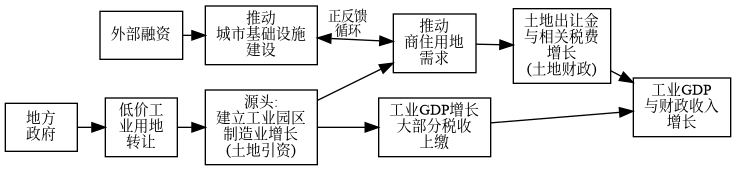
\includegraphics[width=0.9\textwidth]{figures/before08.png}
  \caption{\label{fig:bf08}2008年以前工业增长、土地财政与地区经济增长(可持
    续) }

  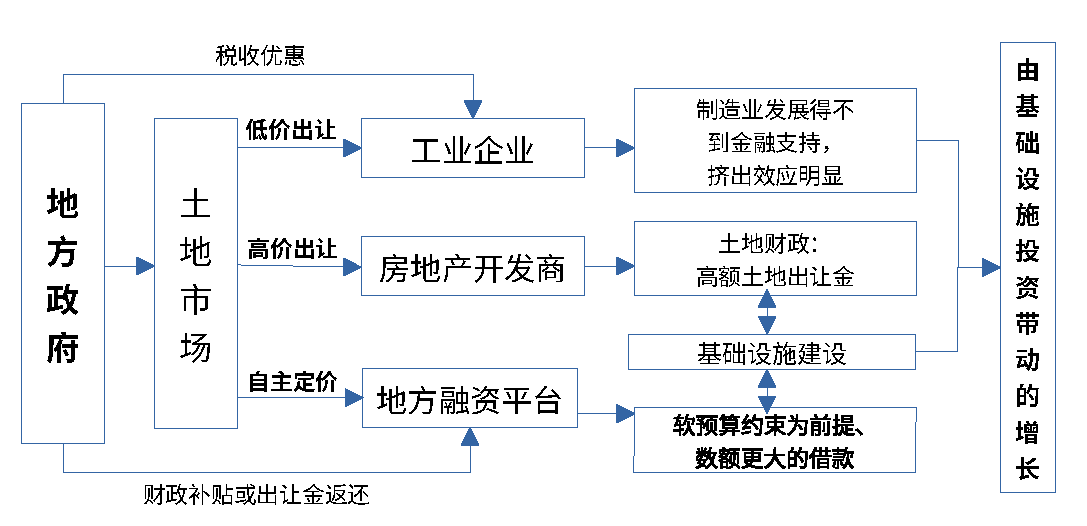
\includegraphics[width=0.9\textwidth]{figures/after08.pdf}
  \caption{\label{fig:af08}2008年后软预算约束与地区经济增长(不可持续) }
  \capsource{范剑勇\qquad《四万亿如何改变了中国经济增长动力》}
\end{figure}

据范剑勇\cite{fanjianyong}:
\begin{quotation}
  2008年之前,中国是硬预算约束条件的土地财政模式(见\cref{fig:bf08},而2008年
  之后,是软预算约束条件下的土地金融模式(见\cref{fig:af08}。2008年之前,经济
  增长的动力是“制造业+房地产”两个轮子一起转,2008年之后是偏向以基础设施为主
  的单轮驱动。
\end{quotation}

详细论述可见范原文,不再赘引。4万亿之后的土地金融历史,就本书所占角度来说,未发生
明显本质转变,也不再赘述。

\subsection{土地置换制度}

本小节几乎照摘周飞舟和谭飞智所著《当代中国的中央地方关系》。

自改革开放以来,我国工业化、城镇化推进速度越来越快,大量耕地农用地被占用是土
地财政\footnote{“土地财政”四字为笔者所加。}发展的必然要求。尤其是进入21世纪以来,
各地土地财政带来大拆大建,形成规模不小的失地农民群体,频发的群体性事件成为危
害社会稳定的重要因素。自中央层面来看,基于保障\textbf{国家粮食安全}以及维持改革以来
确立的家庭联产承包责任制的基本经营组织方式的要求,实行严格的耕地保护制度,以
占补平衡为代表的系列政策应运而生,\textbf{18亿亩耕地红线}作为一项政治任务贯穿而下,
实行一把手问责制。

\subsubsection{耕地占补平衡}

1997年4月,中共中央国务院发布11号文《关于进一步加强土地管理、切实保护耕地的通
知》,明确提出省(区市)必须保持耕地总量动态平衡的要求,同时确定了实行占用
耕地与开发复垦\footnote{土地复垦是指对生产建设活动和自然灾害损毁的土地,采取整治措施,
  使其达到可供利用状态的活动。}挂钩的政策,首次明确提出“耕地占补平衡”的概念。

随后在1998年8月,《中华人民共和国土地管理法》再次修订,明确提出“实行占用耕地
补偿制度”,要求占用耕地与开发复垦耕地相平衡。

1999年2月4日,《关于切实做好耕地占补平衡工作的通知》(国土资发〔1999〕39号)要
求确保建设占地“\textbf{占一补一}”,逐步实现耕地占用的\textbf{先补后占、占优补优、不补不
  占}。自此,耕地占补平衡政策开始在全国各地大规模实施。

2006年以前,占补平衡考核采取的是“\textbf{算大帐}”的方法——以区域为单位,考核区域内
的总占总补平衡。这种方法存在的漏洞是,很多建设用地项目并没有实现法律所规定的
占补平衡,建设用地占用耕地项目单位的补充耕地与土地开发整理脱钩。同时,由于区
域内的占补平衡考核仅仅关注于数量,一些建设项目\textbf{占优补劣}的现象比较突出。

2006年6月8日,国土资源部第3次部务会议通过了《耕地占补平衡考核办法》,于当
年8月1日起施行。“耕地占补平衡考核,\textbf{以建设用地项目为单位进行}”“耕地占补平
衡,实行占用耕地的\textbf{建设用地项目与补充耕地的土地开发整理项目挂钩}制度。”不再
采取大锅饭式的算大账。这一管理思路,为后来的增减挂钩所延续,即采用“\textbf{封闭运
  行}”的项目制运作模式,

随着工业化、城镇化的大势所趋,\textbf{“保耕地红线”成为地方政府沉重的政治负担和资金负
担。}耕地占补平衡政策自出台以来,在各地具体实施过程中主要存在:耕地的“\textbf{实占虚
补}”;补充耕地的“\textbf{实优虚劣}”以及\textbf{农地非农化和非粮化}的风险。耕地占补平衡制度实
行以来,各地实际工作中建设占用耕地长期以“先占后补”和“边占边补”方式为主,
加上对补充耕地的监督力度不够,导致建设占用耕地占而不补、占多补少的问题经常发
生。国土资源部因此颁布《关于进一步加强土地整理复垦开发工作的通知》,规定
从2009年开始,除国家重大工程可以暂缓外,非农占用耕地全面实行“\textbf{先补后占}”。

% 从地方政府角度出发,其更多的是从如何提高土地生产效益的角度出发的,因此如果单
% 纯地维持原有以粮食为主的种植结构难以达到提高效益的目的,转变生产结构成为必然
% 的选择,农地非农化、非粮化在所难免。所谓粮食安全的担忧也并非地方所考虑的问题。
% 在这一点上,中央与地方之间的矛盾凸显。

由于耕地的开垦整理需要一定的工程周期,因而由“先占后补”到“先补后占”的转变,
开启了\textbf{耕地占补平衡指标化}的进程,各地纷纷建立\textbf{占补平衡指标储备库}。提前储
备补充耕地,需新增建设用地时再从库中支取“指标”。

% 中国耕地红线粮食战略安全和土地金融的交织摩擦,使地区\textbf{狂热开发}建设用地的意
% 图受限\footnote{此句为笔者所加。以中国为一整体的角度来考虑,各地重复建设、大干快上,
% 工业用地扭曲的拿地或租赁价格、房地产的癫狂实属狂热无疑。},尤其是经济发达地
% 区与产粮大省更加受限于补充耕地资源较少。

% 从另一各方面来说,耕地红线也使可转化为新增建设用地的农地更加稀缺,加重了土地
% 金融的严重程度。\footnote{此句为笔者所加。}

\subsubsection{土地置换与指标折抵}

中央、省、市、县、乡五级政府的五级规划与年度建设占用耕地计划指标等限制了各级
地方政府对于新增建设用地、发展土地金融的强烈渴求,与中央严格土地制度框架出现
较尖锐矛盾,违法占地屡禁不止,中央政府为此开了以农用土地整理换取新增建设用地
的“口子”。

1999年10月,《国土资源部关于土地开发整理工作有关问题的通知》(国土资发
〔1999〕358号)提出土地置换和指标折抵。

\begin{description}
\item[土地置换] 促进农村居民点向中心村和集镇集中、乡镇企业向工业小区集中,选定新
  址\textbf{建设需要占用其他耕地}时,可以与腾出来的\textbf{旧址整理后增加的耕地}进行置换,实行
  这种方式置换的其建设用地\textbf{不占用年度建设占用耕地计划指标}。


\item[百分之六十指标折抵] 实现耕地占补平衡的地区,可以用通过土地整理\textbf{新增耕地面积
  的百分之六十指标},向上级土地行政主管部门申请一定数量的\textbf{预留建设占用耕地指标},
  用于本地区必需的非农建设。但必须按规划用地,并要严格检查,适当控制。
\end{description}

这两项政策“指标的使用并\textbf{不占用当年的年度建设用地指标},因而受到各地方政府的
欢迎……也是城乡建设用地增减挂钩政策出台的前奏”。

但地方政府仍感受到五级区域对于发展建设用地限制较大:发达地区可供补充耕地量匮
乏,不能满足新增建设用地需求;一般为10--15年的土地规划无法更好预见未来发展,
不可占用基本农田\footnote{基本农田:为了切实保护耕地,国家把按照一定时期人口和社会经
  济发展对农产品的需求,以及对建设用地的预测而确定的\textbf{长期或一定时期内不得占
    用的耕地}称为基本农田。}使大块建设用地项目难以落地。于是一些省开始省内跨
区域操作,实现了较为系统性变通的是浙江省,一些人称之为“\textbf{浙江模式}”。简而言
之就是浙江省将一些指标统筹在省或市以内,不下沉分解至各县各乡;并且各市之间可
以交易指标,落后地区大量土地整理用以补充耕地,发达地区向落后地区购买耕地指标
专心发展建设用地。详细了解可见汪晖、陶然《论土地发展权转移与交易的 “浙江模
式”——制度起源, 操作模式及其重要含义》。


\begin{quotation}
  对浙江在土地发展权转移和交易上的改革探索,不仅学界有论述质疑浙江的做法
  是\textbf{规避中央政府基本农田审批权和新增建设用地土地有偿使用费,导致基本农田质
    量下降和建设用地总量失控}(谭峻等,2004 年),中央政府也存在不少担心。

  欠发达地区为了折抵指标过度投资土地整理,甚至在新增耕地比例上弄虚作假,或发
  达地区通过购买折抵指标无限制扩张城市和工业园区用地。

  浙江省基本农田集中置换和易地代保政策\footnote{即基本农田易地代保:简而言之,发达市
    县有偿购买落后市县的基本农田,以便消除本市县相应面积、质量的基本农田保护,
    新增大块连续建设用地。}在国土资源部《关于进一步采取措施落实严格保护耕地制度的通
  知》(国土资发〔2003〕388 号和国务院办公厅《关于深入开展土地市场治理整顿严格
  土地管理的紧急通知》(国办发明电〔2004〕20 号)公布后停止执行;折抵指标政策也
  在《国务院办公厅关于严格执行有关农村集体建设用地法律和政策的通知》(国办发
  〔2007〕71 号)颁布后停止执行。\cite{wangzhejiang}
\end{quotation}


\todo[inline]{浙江模式其实就是市县级土地金融的扩大版,大国大城其实就是浙江模
  式的扩大版?参考LaTeX源文件中以下被注销部分。自由派认为行政主导要继续让位
  给市场自由流动。}

\subsubsection{城乡建设用地增减挂钩}

\begin{quotation}
  2004年10月21日国务院下发《关于深化改革严格土地管理的决定》,“实行最严格
  的土地管理制度……鼓励农村建设用地整理,\textbf{城镇建设用地}增加要与\textbf{农村建设用
    地}减少相挂钩”。

  (4年陆续增加试点后,)2008年6月27日,国土资源部印发《城乡建设用地增减挂钩
  试点管理办法》,明确提出了“城乡建设用地增减挂钩是指依据土地利用总体规
  划,\textbf{将若干拟整理复垦为耕地的农村建设用地地块(即拆旧地块)和拟用于城镇建
    设的地块(即建新地块)等面积共同组成建新拆旧项目区}(以下简称项目区),通
  过建新拆旧和土地整理复垦等措施,在保证项目区内各类土地面积平衡的基础上,最
  终实现\textbf{增加耕地有效面积,提高耕地质量,节约集约利用建设用地,城乡用地布局更
  合理}的目标。”其实仔细比较增减挂钩政策与之前我们所分析的建设用地指标置换政
  策其在表述上和本质上相类似,而这也反映了中国改革中政策制定的延续性和探索性。

  同时138号文批复下达了第二批试点项目(共10246公顷,合15.368万亩),项目区以
  项目区备选方式下达。2009年3月5日,《国土资源部关于2009年第一批城乡建设用地
  增减相挂钩周转指标的批复》(国土资函[2009]299号),对河北、内蒙古、辽宁、吉
  林、黑龙江、福建、江西、河南、湖南、广东、广西、云南、宁夏13省(区),批复
  下达周转指标15.275万亩(合10183.3公顷)。2013年10月23日下午,国土资源部部长、
  党组书记、国家土地总督察姜大明主持召开第15次部长办公会,审议并原则通
  过2013年城乡建设用地增减挂钩指标分解下达方案,共批准29个省份开展增减挂钩试
  点,全国共安排城乡建设用地增减挂钩指标90万亩。\cite{yangdi}
\end{quotation}

\begin{figure}[htbp!]
  \centering
  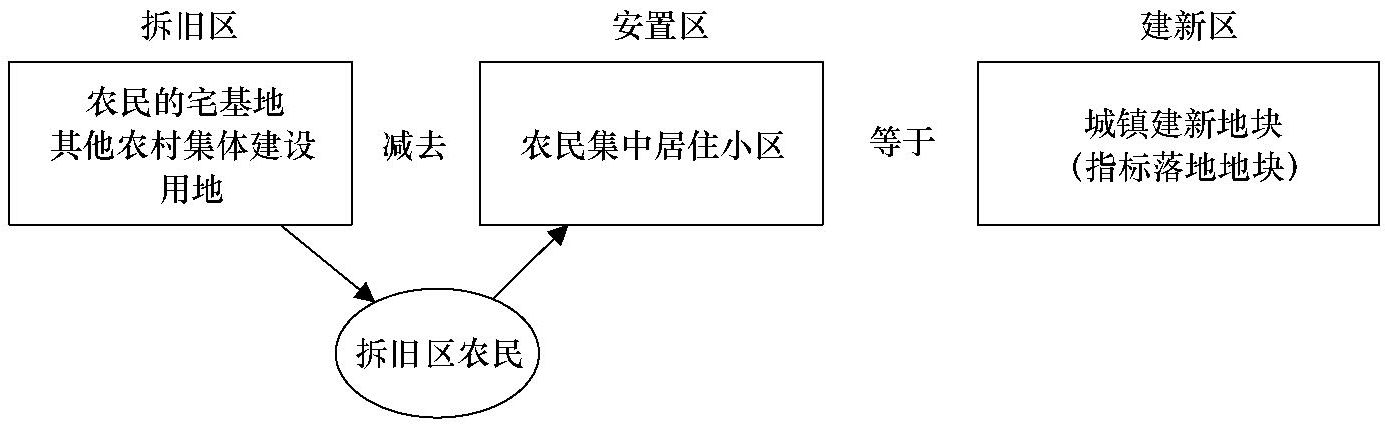
\includegraphics[width=0.9\linewidth]{figures/zengjianguagou.jpg}
  \caption{\label{fig:zengjianguagou}城乡建设用地增减挂钩政策示意图}
  \capsource{周飞舟、谭飞智\quad 《当代中国的中央地方关系》}
\end{figure}

\begin{quotation}
  指标计算公式:增减挂钩周转指标=拆旧区总面积-农民集中居住小区占地面积=项目区
  中建新地块可占地面积(见\cref{fig:zengjianguagou})。所谓“\textbf{周转指标}”其
  在实质上是一种指标“\textbf{预借}”或“\textbf{透支}”制度。拆旧复垦是一项非常庞大的工
  程,短期内难以完成,因此不需要拆旧区完成耕地复垦工作之后,建新区才能够进行
  城镇开发建设。也正是在这个意义上才有了指标“\textbf{周转}”的概念,一般要求,指标
  三年归还。

  增减挂钩的根本意义在于:开辟了一个独立于每年新增建设用地指标严控体系以外的
  指标来源,为城镇发展提供“不占指标”的“计划外”土地资源,且规模逐年增加。\cite{yangdi}


  截至2013年底,全国共有29个省(自治区、直辖市)被纳入了试点范围,共下达周转
  指标约90万亩。

  2017年4月,增减挂钩再出新政,在《关于进一步运用增减挂钩政策支持脱贫攻坚的通知》
  中,明确允许省级贫困县的增减挂钩节余指标在\textbf{省域范围内}流转使用,进一步释放了
  政策红利。为了落实国家乡村振兴战略,2018年3月,国务院办公厅印发了《城乡建设用
  地增减挂钩节余指标跨省域调剂管理办法》,规范了“三区三州”及其他深度贫困县增
  减挂钩节余指标\textbf{跨省域调剂},助力落实国家精准扶贫、绿色发展的战略。至此,增减
  挂钩先后两次完成政策升级,从省域内流转到跨省调剂,逐步拓展政策适用范围。这一
  阶段增减挂钩政策更加强调以人为本,致力于城乡区域协调发展和社会公
  平。\cite{zengjianzongshu}
\end{quotation}

据《央地关系》,不管是政策实质还是地方需求,对新增耕地并无多少刺激,只是满
足“占补平衡”即可。如\cref{fig:zengjianguagou},为获得更多新增建设用地,地方
倾向于减少农民集中居住小区占地面积,显而易见的方法是“农民上楼”——楼房可以
在单位占地面积提供更大容积率、容纳更多被增减挂钩析出的农民;并采用合村并居等
方法,以便进一步减少成本、扩大新增建设用地指标。

中央中央政府面临对地方监管失控的风险。一方面土地金融下,地方为GDP考核机制不满
足于中央给定的增减挂钩指标,为获得更多新增建设用地或直接将用地指标出售给其他地
方,对大量村庄违规改造;另一方面中央为维持地方发展的积极性及活力,又不得不逐
年扩大试点范围和规模。

增减挂钩以项目制方式向下推进,中央资金以项目形式向下转移,各级地方政府必须要
有相应的配套资金和政策支持,地方政府继续高额举债以及引入社会资本成为必然。债
务压力迫使地方忽视了反哺农业、农村、农民,仍倾向于以建设养建设;可同时进行的
拆旧和建新在极端情况下也会停滞或缓慢发展,造成各种不安定因素积累发酵;地方也
面临和社会资本的博弈;合村也带来更多政治管理矛盾。

起初农村拆迁矛盾多因行政强制指令下补偿不足,农地价征收城低价出售,城乡二元对
立有所加重,有损村民利益。随着政府日益重视农民权益问题,拆迁补偿已有较大实质
性改观。但随着市场经济边沁利己的日益深入人心,土地金融的日益发展,使土地成为
全民全社会共同参与的虚假繁荣市场,增减挂钩成本日益提高,越发加重了风险。


土地金融造成地方各自为政,产业结构相同且全副该,重复建设,狂热追求新增建设用地,农民上楼,大额投资等等


韩长赋: 中国农村土地制度改革

耕地退化、污染严重,一些地方占好地、补坏地,占水地、补旱地,2016 年全国优高
等耕地面积仅占 29. 5%。




反面论述
https://www.aisixiang.com/data/115819.html
赵燕菁:从土地金融到土地财政:资本的胜利、有为的政府与城市的转型

※※※※※※※※※※※※※※※※※※※※※※※※※※
https://bfi.uchicago.edu/wp-content/uploads/2022/02/BFI_WP_2022-24.pdf

文献中的典型观点是,住宅用地出让主要是地方政府增加收入的一种方式,而工业用地
出卖主要是为了补贴产业、刺激经济增长、支持劳动力需求。

中国的土地市场具有相当大的工业折扣:工业区用地比住宅用地便宜一个数量级。与以
产业补贴或促进产业增长为中心的解释相反,我们强调了未来土地税收的重要性,并发
现地方公共财政激励措施可以在很大程度上合理化这种价格差距。在“土地融资”制度
下,土地出让是中国地方政府的重要收入来源。研究表明,在中国,地方政府作为垄断
性土地销售者,面临着住宅用地或工业用地供应之间的权衡,这取决于工业和住宅用地
销售收入的不同时间分布、地方政府的财政约束以及地方政府与其他各级政府分享税收
的程度。

公司税收收入和土地出让收入;2019年,这两个数字分别约为8.7万亿元人民币和7.3万
亿元人民币.2工业用地产生持续的未来税收流动,因为工业企业缴纳增值税和所得税,
以及各种费用。由于中国没有住宅物业税,住宅用地销售只会暂时增加房屋开发商缴纳
的税款.3这意味着地方政府面临着一个选择,即出售前期收入较大的住宅用地和出售工
业用地,因为工业用地支付的税收现金流比实际收入更持久。

这种动态的观点意味着,大量的前期工业用地折扣并不一定意味着政府正在通过廉价土
地系统地补贴工业。事实上,我们表明,在调整住宅开发商缴纳的税款后,来自工业用
地的税收流动可以定量补偿前期工业用地折扣。我们还提供了地方政府的融资需求影响
土地分区的因果证据,表明地方公共财政在通过土地分配渠道塑造中国经济增长路径方
面发挥着被低估的作用

我们从一个概念框架开始,分析推动工业用地而不是住宅用地供应均衡回报的力量。我
们考虑的是地方政府,其目标是最大化其财政收入的现值。除了全部属于地方政府的前
期土地销售收入外,住宅用地还产生了由房屋开发商支付的一次性税款,而工业用地则
产生了工业税的持续现金流,并与中央政府共享。在均衡状态下,由于未来的税收优惠,
当地政府愿意以较低的价格出售工业用地。该框架指出了两个简单且可衡量的汇总统计
数据。首先是工业折扣,即工业用地和住宅用地之间的价格差异。第二种是工业用地销
售的内部收益率(IRR),计算为贴现率,折现率等于工业和住宅用地销售的所有现金
流的现值

※※※※※※※※※※※※※※※※※※※※※※※※※※

就像许多其他国家一样,中国也有严格的分区限制。正如Chen等人(2018)所强调的那
样,划为住宅用途的土地的售价大约比划为工业用途的土地高出十倍。2019年,中国住
宅用地平均价格为3,619元/平方米,工业用地平均价格为304元/平方米。我们将住宅用
地和工业用地之间的这种价格差异称为工业用地折扣(或工业用地互换)。

※※※※※※※※※※※※※※※※※※※※※※※※※※

地方政府从土地中获取融资有两条直接渠道:一是土地财政,即通过出让国有土地(主
要是商服用地和住宅用地)50至70年的使用权来获取级差地租;二是土地金融,即将土
地注入地方融资平台来撬动资金为城市建设融资。

已有研究表明,土地财政和土地金融相结合的以地融资模式催生出一个高效的融资体系,
极大推动了近二十年来的中国经济增长,特别是与房地产和基建相关(包括钢铁、水泥)
的重工业部门得到了飞速发展,居住环境和基础设施的改善又进一步促进了地价和房价
的升值,为下一轮以地融资创造了有利条件。这样的正向反馈机制使得中国自1998年以
来一直处于投资驱动型的增长阶段。

如果说曾经的以地融资模式主要依赖土地财政,那么如今,随着部分地区土地资源的告
罄和征地补偿标准的提升,一些地方政府对土地财政的依赖开始减退,而对土地金融却
愈加青睐。由表1可知,越是土地资源稀缺的地区(东部地区),土地抵押贷款规模越
是高于土地出让规模,而对北上广这样的一线城市而言,土地抵押与土地出让的比值更
是高于东部地区的平均水平。

图1显示,2003至2010年间,出让成本占比基本维持在六成左右,但在2011至2018年间,无论是土地出让成本的规模还是其占土地出让毛收入的比重都呈加速上升趋势,甚至到了2018年,土地出让成本占土地出让毛收入比重已接近九成。

从征地规模的角度亦可佐证土地出让成本在2010年前后出现了飘升的现象。图2显示,农用地和总的土地征收规模在2011年之前处于上升区间,但在2011年后呈逐年加速下滑的态势,这恰好是土地出让成本开始飘升的年份(参见图1)。迅速缩小的征地规模表明,未来国有土地的出让规模将大幅缩减,利用土地财政进行创收的空间将被进一步压缩。

1994年的税收分享改革,该改革减少了地方政府在许多税收收入来源中的份额,同时并没有减少他们的支出需求。要回答“为什么土地金融在中国(到目前为止)有效运作”要复杂得多。在这方面,了解其促进土地金融体系盈利能力的制度基础是很重要的。首先,地方政府被指定为地方城市LUR的垄断提供者。因此,当一个城市提出购买农村土地并将其转换为城市土地时,它不会面临来自其他实体的竞争。此外,支付的补偿是基于当前(农业)用途的土地价值,而不是未来城市用途。地方政府回购、分配或出售的城市土地利用率并将其转换为新的土地利用率时,也适用类似的规定。这种安排使城市政府能够获利,直到最近,土地价格的暂时上升趋势加剧了这一点。值得注意的是,支撑土地金融体系的丰富制度框架既有法律、官方文件等显性规则,也有在实践中具有影响力的隐性规范。其中一些细节在现有文献中似乎没有得到适当的承认,并可能导致对该系统的误解。希望我们的分析能够更清楚地说明该系统在中国联邦体系中的运作方式

自1980年代以来,中央和地方政府在中国经济中扮演的角色已经很明确——中央政府负责规划和监管,而地方政府则负责在地方层面实施这些法规。

从1980年到2020年,地方政府在国家一般公共预算中的份额从45.7\%增加到85.7\%,而同期收入在一般公共预算中的份额从75.5\%下降到55.5\%。为了弥补收支缺口,地方政府依靠中央政府补贴、债务融资和土地融资。

1994年实行的税制改革在随后的几年中对土地融资产生了巨大的溢出效应。改革规定,中央政府将把所有与土地有关的税收分配给地方政府。这包括土地价值税、城市土地使用税、耕地占用税、土地增值税、契税(财产转让税)和一般财产税。更重要的是,土地出让的所有利润都转移到了地方政府。

这一新制度为地方政府增加了土地出让收入提供了强大的动力。从2000年到2020年,地方政府土地出让收入占总收入的比重从5.9\%提高到42\%。如果将其他相关的土地税也考虑在内,土地收入占地方政府总收入的一半以上(52\%)。

o“通过信用制度,未来的收益可以贴现到今天,使得资本的形成方式得以摆脱对过去积累依赖,转向预期收益。”“中国城市伟大成就背后的真正秘密,就是创造性地发展出一套将土地作为信用基础的制度——‘土地财政’。”


土地财政是指政府出让国有土地使用权收入,及与土地有关的税收如耕地占用税、土地增值税等,这都是有法律、制度依据的。土地金融是指政府拿土地做抵押,向银行贷款,属于政府负债。这样做,没有法律依据,是打了制度的“擦边球”,因为制度允许政府作为国有土地所有权的代表经营土地。


但是当市场经济更多要求个人为个人负责,并将此观念植入人心时,一些原住民的死缠
烂打、坐地起价也就避无可避,因此拆迁往往要大费周章。突破口似乎只有合法或非法
的“暴力”。

合法暴力,可以宣称土地权利不归属于抗拒拆迁的人员,如印度最高法院声称孟买等地
贫民窟的长期居民是土地的非法占有者,没有权利要求拆迁赔偿,\textbf{承认获赔权等于奖
励盗窃行为};美国滥用征地权,把合理建筑中的长期居民赶走,鼓励高层建筑;声称
土地为集体所有,集体才是土地权利所有者,而非小部分人。

非法暴力,如20世纪90年代韩国首尔开发商雇佣黑帮“相扑似的打手”暴力拆迁;印度
西孟加拉邦南迪格莱姆地区的冲突惨案等。


《从沸腾到癫狂》

北京2005~2009年政府公布的商品房住宅建设用地计划供给指标为7130公顷,非商品住
房建设用地指标为1320公顷,两者的比重为5.4∶1。而实际供给的情况则是,商品房住
宅用地(招拍挂)2394公顷,完成计划数的33.6%,供地差额为4736公顷;非商品住宅
供地1283公顷,完成97.20%,扣除商品房中的配建,非商品房完成率为103%。这些土
地为享受经济适用住房政策的用地,约为商品房用地的2倍,由特定单位使用了。商品住
宅用地与非商品住宅用地的面积相加,可以计算出商品住宅用地在全部住宅建设用地中
的比重仅为28.3%。



任志强认为,市场中计算出的商品住宅平均销售价格仅为这28.3%的住宅销售价格,而并非北京市的住宅实际价格。如果用地中的平均容积率相等,且大部分经济适用住房和享受经济适用住房政策的住房价格为4500元/平方米,则北京市的一手房销售价格约仅为6200元/平方米。

任志强说,虽然那些低价的定向住房没有向社会公开销售,比如分给了国务院事务管理局,再分配给中央或国务院的各机关、管理机构以解决公务员的住房、进京干部的住房、老干部的住房等,但这些住房也是解决北京的住房问题,所以,应该在统计时计算进来进行平均。

房真实房价平均仅为6200元/平方米。而根据北京市统计局、国家统计局北京调查总队公布的《2009年北京市房地产市场运行情况》,2009年第四季度,四环路以内商品住宅期房销售均价为25907元/平方米。

6200元/平方米与25907元/平方米,为什么两者的差距如此之大?



任志强如是写道:



北京2005~2009年政府公布的商品房住宅建设用地计划供给指标为7130公顷,非商品住房建设用地指标为1320公顷,两者的比重为5.4∶1。而实际供给的情况则是,商品房住宅用地(招拍挂)2394公顷,完成计划数的33.6%,供地差额为4736公顷;非商品住宅供地1283公顷,完成97.20%,扣除商品房中的配建,非商品房完成率为103%。这些土地为享受经济适用住房政策的用地,约为商品房用地的2倍,由特定单位使用了。商品住宅用地与非商品住宅用地的面积相加,可以计算出商品住宅用地在全部住宅建设用地中的比重仅为28.3%。



任志强认为,市场中计算出的商品住宅平均销售价格仅为这28.3%的住宅销售价格,而并非北京市的住宅实际价格。如果用地中的平均容积率相等,且大部分经济适用住房和享受经济适用住房政策的住房价格为4500元/平方米,则北京市的一手房销售价格约仅为6200元/平方米。

任志强说,虽然那些低价的定向住房没有向社会公开销售,比如分给了国务院事务管理局,再分配给中央或国务院的各机关、管理机构以解决公务员的住房、进京干部的住房、老干部的住房等,但这些住房也是解决北京的住房问题,所以,应该在统计时计算进来进行平均。

按照任志强的说法,商品住宅用地28.3%之外的用地,一部分被用于建设北京市和在京中央和国家机关的公务员住房,他们的名称可以是两限房、经济适用住房、享受经济适用住房政策的住房、合建房、自建房中的任何一个。当然,也不排除这些公务员在享受了经济适用房等保障房以后,仍然自掏腰包去购买商品房。



地产商什么时候成为一个阶层了?正统的社会学者肯定要嘲笑我的无知。他们会教育我:你可以称他们为一个群体,一个集团,就是不能称其为一个阶层。是啊,连天天挂在老百姓嘴边的“中产阶层”都未获正式承认,哪里来的地产商阶层?

为什么地方政府会产生对土地财政像网瘾一样的依赖?根子在于土地招拍挂制度。这是一个影响力仅次于1998年房改的制度,并将继续对房地产市场和地方财政产生决定性的导向作用。

招拍挂制度必然导致地价上涨,而地价上涨则必然推动房价上涨。只要招拍挂制度存在,地王的产生就不可避免。地产GDP主义是被一种强力制度牢牢地固定住的地方政府价值取向。

并于2010年6月后成功超过日本成为全球第二大经济体,其中房地产贡献良多。据国家统计局数据,2010年,全国房地产开发投资完成48267亿元,同比增长33.2%;全国商品房销售面积10.43亿平方米,同比增长10.1%;商品房销售额约为5.25万亿元,同比增长18.3%。

因此,即使是全面调控的2010年,房地产的地位也丝毫没有下降。自从1998年实行住房商品化以后,GDP对房地产业的依赖就逐步形成,以至于到了离不开的地步,关键时刻总是要靠房地产“挺身救主”。实事求是地说,这方面没有一个产业能比得上房地产。

以上是从全局,从中央政府层面来说。对地方政府来说,房地产就更重要了。土地财政,这已成为大多数地方政府最重要的财政收入来源。城市形象、政绩工程也离不开地产商和房地产业,许多地方的道路等基础设施都是由地产商修建的。

2004年以来,地方政府体会到土地公开出让的无可替代的好处,招拍挂出让普遍推行。而招拍挂一般是净地出让,拆迁是政府的事。而土地收益当然要远大于拆迁补偿款,否则他们是没动力拆的。地方政府为了尽快把土地卖出去,就会做出强制拆迁、暴力拆迁的事情来。


1991年实施和2001年修改的《城市房屋拆迁管理条例》。依此条例,地方政府贴一纸拆迁通知,在被拆迁的房屋上圈画一个大大的“拆”字就够了。居民不肯搬迁?先有房管部门行政裁决强制拆迁;还不服?接着可能就是法院裁决直接带着铲车来。许多地方连行政和法院裁决都懒得走,直接派消防队和铲车来。这才叫雷厉风行,超级效率。中国城市面貌的日新月异,城市建设的突飞猛进,该《条例》立了大功。

不少专家称这部条例是一部恶法,出台伊始就呼吁修改之。修改后的条例草案数易其稿,并分别于2010年1月29日和12月15日分两次向全社会公开征求意见,这在我国立法史上前所未有,也从一个侧面证明了拆迁所涉及的利益极为纷繁复杂。北大法学教授说,新的条例难以正式出台,主要就是遭遇到地方政府的强烈阻挠。千呼万唤之后,2011年1月21日,国务院正式出台《国有土地上房屋征收与补偿条例》。



2007年1月,国家税务总局曾要求各地税务机关严格土地增值税清算,此举曾令开发商大
为紧张。然而,金融危机呼啸而来,经济形势急转直下,这一号称“革房地产商命”的
税收政策再一次不了了之。赵晓等吁请严征土地增值税,以“100%预征、100%清
算”来遏制新一轮楼市疯狂。

到遏制投机的作用一样,对地产商和投资者个人尤其是地产商征收土地增值税,亦未能成为阻止涨价的动力。

事实上,土地增值税更像是为地方政府找到了一个新的税收来源,虽然这可能并非该税种设立的初衷。

严格征收土地增值税,能够为地方政府带来多大的税收?实事求是地说,2010年以来的保障房建设规模,令人惊讶。

很难想象,如果没有2008年10月推出的4万亿政府投资计划,保障房建设会有今天如此庞大的规模。我并不是说加快保障房建设是为了应对国际金融危机而采取的措施,而是说,保障房建设规模如此庞大,沾了4万亿“救市”资金的光。

2008年11月5日召开的国务院常务会议,确定了进一步扩大内需、促进经济增长的十项措施(“出手要快,出拳要重”的说法由此而来),第一条就是加快建设保障性安居工程。在4万亿投资里,坊间曾有保障房占8000亿元、9000亿元的说法,但并不准确。

根据国家发改委主任张平2009年3月8日在十一届全国人大二次会议新闻发布会的介绍,在4万亿政府投资计划中,保障性住房投资总规模为4000亿元左右。从张平的介绍来看,保障房包括廉租房、林区、垦区、煤矿棚户区改造,但没有提到限价房、经济适用房、公共租赁房等的投资,所以实际投资规模要远远大于4000亿元。

2008年受国际金融危机影响,除北京等极个别城市外,各地对保障房投入仍然不足。真正较大规模的保障房建设是从2009年开始的。

根据2010年3月5日全国“两会”上的《政府工作报告》,2009年中央财政安排保障性安居工程补助资金551亿元,比上年增长2倍。新建、改扩建各类保障性住房200万套,棚户区改造解决住房130万套。从中央财政投入看,增幅甚大。那么,2009年地方对保障房的投入有多少呢?

全国人大常委会专题调研组2009年10月月底披露的一份调查报告显示,截至当年8月月底,全国保障性住房建设完成投资394.9亿元,完成率仅为23.6%。以此推算,当年全国保障房投资计划大约为1600亿元。减去中央财政投入的551亿元,地方即使足额完成投入计划,亦不过1050亿元。

财政部2007年11月颁布的《廉租住房保障资金管理办法》规定,应从土地出让净收益中按照不低于10%的比例安排用于廉租住房保障资金。2009年全国土地收益实际到账14239亿元。也就是说,2009年各地仅廉租房就应投入1424亿元。加上公共租赁房、经济适用房和限价房,总投入至少应该倍增。而事实上,2009年各地保障房实际投入额尚不足财政部规定的廉租房投入额,遑论加上公共租赁房、经济适用房和限价房。

当然,从全国“两会”《政府工作报告》公布的数据看,2009年全国保障房建设任务是完成了的。330万套保障房的投资,应远远超过1600亿元。

2010年的保障房建设规模更加惊人。根据住房和城乡建设部的安排,2010年全国计划建设廉租住房、公共租赁住房等300万套,改造各类棚户区住房280万套,农村危房改造试点120万户。农村危房改造不计,人们将2010年的保障房任务简称为580万套。从330万套,到580万套,增长超过70%。

https://www.mof.gov.cn/zhuantihuigu/czjbqk2011/czsr2011/201208/t20120831_679821.html
全国土地出让收入管理及使用情况

2007年之前,土地出让收入先纳入预算外专户管理,再将扣除征地补偿和拆迁费用以及
土地开发支出等成本性支出后的余额缴入地方国库,纳入地方政府性基金预算管理。
从2007年开始,国家对土地出让收入管理制度进行了改革,将全部土地出让收入缴入地
方国库,纳入地方政府性基金预算管理,与公共财政预算分开核算,专款专用。土地出
让收支纳入政府性基金预决算编制范围,实行预决算管理制度。每年第三季度,国土资
源管理等有关部门按照相关规定编制下一年度土地出让收支预算。每年年度终了,国土
资源管理等有关部门按照规定编制上年土地出让收支决算。同时,按照规定程序向同级
人民政府报告,政府依法向同级人大报告。

% 新自由主义,彻底的附庸
% 杨继绳《中国改革时代的政治斗争》
% \begin{quotation}

% 新左派认为,目前中国的改革越来越走向自由主义所倡导的模式,中国正在进入资本主义全球体系。当前“中国社会的各种行为,包括经济、政治和文化行为甚至政府行为,都深刻地受制于资本和市场活动。”“80年代中国的启蒙思想所许诺的‘好社会’不仅没有伴随经济市场化而到来,市场社会本身呈现了新的、在某种意义上来说是更加难以克服的矛盾。”(汪晖:《当代中国思想状况和现代性问题》)新左派满怀忧虑地问道:“我们今天这个世界究竟是谁在统治,是人民呢还是寡头?是权力呢还是资本?这是需要深思的。在全球化潮流下,跨国公司正在系统地、有步骤地剥夺世界各国人民的民主权利,正在把我们这个世界带向奴役之路。如果看不到这一现实的威胁,恐怕就谈不上懂得民主。“(韩德强,2000)

% 自由派认为,目前中国虽然存在种种问题,但正在从不合理的体制走向合理的体制,走向人类文明的主流。他们所说的人类文明的主流就是以英美为标志的价值体系和社会制度。“对于自由主义立场而言,中国向市场经济转型问题再多再严重,也只能硬着头皮向前走,决不能走回头路,决不能返回衣、食、往、行都被人包办,种什么,造什么,卖什么都得等上级指示的那种日子。”(徐友渔:《自由主义与当代中国》)

% 对当前的社会结构的变化,自由主义者持乐观的态度。他们认为,20年的改革,已经在政府之外开始出现了新的社会结构,这种新的社会结构可能是将来中国的市民社会和公共领域的雏形,在中国的社会发展中是将成为一支重要力量。因此,让这种新的社会结构进一步发展是一条必由之路。新左派认为上述看法是当今既得利益集团虚构的神话,他们认为,这20年所形成的不是中间阶层,而是新生的资产阶,是垄断精英,垄断精英是改革中社会不公正的既得利益者,是需要限制的、而不是应当鼓励发展的阶层。

% 中国正处在十字路口,搞得好,就可能建成一个民主、法治的社会,搞不好,就可能形成一个金权、家庭统治的新型专制制度。就像某些南亚和拉美国家一样。这是两派一致的看法。但是,新左派认为这种危险在于市场霸权和垄断精英,自由主义者认为这种危险在于没有得到改革的原有的权力结构,在于中国两千多年相沿成习的专制主义。

% 自由主义者把政治权力的无限膨胀看成是奴役民众的力量,新左派把市场力量的无限膨胀看成是奴役民众的力量。
% \end{quotation}


% #+BEGIN_SRC dot :file before08.png :cmdline -Kdot -Tpng :exports results
%   digraph G {
%     rankdir="LR"
%     rank=min
%     ranksep=0
%     node[shape=record fontsize=11]
%     yuan[label="源头:\n建立工业园区\n制造业增长\n(土地引资)"]
%     shangzhu[label="推动\n商住用地\n需求"]
%     jishe[label="推动\n城市基础设施\n建设"]
%     end[label="工业GDP\n与财政收入\n增长"]
%     gongshui[label="工业GDP增长\n大部分税收\n上缴"]

%    外部融资 ->  jishe
%    jishe -> shangzhu[dir=both, label="正反馈\n循环", fontsize=10]
%    shangzhu -> "土地出让金\n与相关税费\n增长\n(土地财政)" -> end

%     "地方\n政府" -> "低价工\n业用地\n转让" -> yuan -> gongshui ->end

%     yuan -> shangzhu
%     {rank=same gongshui  shangzhu}
%   }
% #+END_SRC

%%% Local Variables:
%%% mode: latex
%%% TeX-master: "../main"
%%% End:


\part{人文}
\chapter{生命}

\begin{quotation}
  生命权是最基本,最重要的人权,如果无法充分保障人的生命权,那么一切其它权利
  都是空中楼阁。无端剥夺人的生命,或者肆意对人施加恐吓、虐待和折磨,就是用一
  种非人权的待人方式。任由这种情况发生,个人权利就无从谈起。所以一般各国的刑
  法都将侵害他人生命权的罪行量刑最重。

  生命权是一个人之所以被当作人类伙伴所必须享有的权利。\cite{renquanwiki}
\end{quotation}

\section{关于无国界医生的一场争议}

\begin{quotation}
  无国界医生是一个独立的国际医疗人道救援组织,致力为受武装冲突、疫病和天灾影
  响,以及遭排拒于医疗体系以外的人群提供紧急医疗援助。无国界医生只会基于人们
  的需要提供援助,不受种族、宗教、性别或政治因素左右。
\end{quotation}

传媒、文学作品等往往将MSF成员描绘为在枪林弹雨里冒着极大生命危险抢救难民的英雄。
这是过于煽情而有失偏颇的。MSF医生的生命同样是生命,MSF组织并不会让医生为救人
而面临随时死亡的危险,只会辟出安全区域设立医院为难民实行救治。

知乎网有关于无国界医生蒋励的一张帖子热度较高,文字回复条数过千。题目是,《如
何看待北京医生辞职去阿富汗参加无国界医生?》。\cite{kandaijiangli}

蒋励在北京大学医学部完成八年本硕博连读教育后,顺利入职北京大学人民医院。受师
姐和领导屠铮影响,“2012年参加了无国界医生。2013年3月至6月在无国界医生位于阿
富汗霍斯特的妇产医院工作(同时前往阿富汗的另一MSF中国内地成员——麻醉医生赵一
凡去了昆都士省的外科创伤医院),2014年1月再次去往无国界医生在巴基斯坦蒂默加拉
的医院工作。”,\cite{jiangli}。阿富汗霍斯特医院情况总结如下,床位\textbf{60}张,每
月\textbf{1200多例}分娩,相关医护人员有\textbf{2位妇产科医生,4位国际助产士,2位麻醉医生}组
成,也就是说,这8个人分工协作,24小时不间断的进行每天平均40余例的分娩“流水线
作业”。挽救了极多数量的新生儿和妊娠母亲的生命。

但有关这个帖子的一些回复真是让人完全意想不到,瞠目结舌。其中点赞1700多次、点
赞次数排行第四的匿名帖子反对无国界医生对阿富汗的援助,提倡\textbf{绝育论},“已经生
育三个及其以上孩子的妇女向援助医院请求接生必须以切除子宫或者上节育环作为交换
条件,然后由国际组织建立隔离带,优先为已经绝育的妇女及其子女提供庇护,食物,
医疗和基础教育,把儿童从中剥离出来接受现代教育。”,有帖子发表类似观点“没有
条件接受教育的人就没有出生和生存的权利。”,除此之外,还有“愚善”,“学医救
不了阿富汗”等脑沟回清奇的言论。

在网络上,不止此贴所涉及国家,我们还可以看到,关于罗姆人(吉普赛人)、社会底
层人士的优生学绝育论。这种绝育论宣扬,就缺乏教育和社会资源的群体,或者相比自
己群体拥有更高不和谐的群体——这种水平判定其实只是个人不负责的主观判断,应当
尽量抑制他们彼此间繁殖新生生命,对于正在或已经出生的新生生命,“社会上流人
士”有义务、有必要剥夺新生儿父母的监护权、教育权,让社会特殊的学校或机构行使
监护权、教育权,使他们脱离这个不文明的群体……

\section{“科学”的优生学绝育论}

优生学常是举着科学的旗号,被一些别有用心或者精神脆弱之人利用,行反伦理、反人
类之实,让我们看看优生学在历史上曾被误用滥用的历史吧,以下内容节选自邱仁宗所
著《一本医学家、遗传学家、决策者和立法者必读的书——《从“安乐死”到最终解
决》》\cite{yousheng}:

\begin{quotation}
  1881年Francis Galton提出“优生学”,当时被定义为“通过优化生育改良人种的科
  学” 。于是在北美和欧洲兴起了一场将弱智、残疾、在竞争中处于劣势的人绝育、禁
  止他们第一章探讨种族灭绝的意识形态背景, 即固守“人类不平等”入境的优生运
  动。1907年美国印第安那州颁布了第一部将精神病人、性罪错者、智力低下者、道德
  堕落者和癫痫病人绝育的法律,到了30年代中期已有半数以上的州通过了类似的法律。

  对日耳曼人或德意志人的优良品质深信不疑的德国医生和科学家提出了“种族卫
  生”(Rassenshy giene)概念。

  1920年德国律师Carl Binding和医生Alfred Hoche出版了第一本题为《授权毁灭不值
  得生存的生命》的书。

  正是纳粹政权使种族卫生计划成为现实,它决心保持德意志血统的纯洁性,清理德意志
  的基因库,将“人类不平等”这一思想制度化。1933年7月颁布《 防止具有遗传性疾病
  后代法》,即绝育法,对患有各类精神和肉体疾病的病人实行强制绝育。1933年11月颁
  布《反危险惯犯法》和《安全和改革措施法》, 授权将反社会者关进国营医院,对性犯
  罪实行阉割手术。1935年9月颁布《 帝国公民法》和《德意志血统和尊严保护法》,二
  者统称纽伦堡种族法,正式在法律上排斥犹太人、吉卜赛人、黑人。

  1939年10月,希特勒签署了一份文件,文件称:“一些根据人道的判断被确认为不可治愈
  的病人在确诊后准许被实施慈悲死亡。”

  后来将残疾人安乐死的计划进一步在德国占领区扩大实施。接着大规模屠杀吉卜赛人
  和犹太人,进行所谓“最终解决”,被杀害的人数达600万人。
\end{quotation}

在数年前,这种极端蔑视生命权的言论在中国没有一丁点市场,几乎见不到有人去支持。
如今我们不需要在网络上,就算是在现实中的社交场合,都能听到这些优生学绝育论或
灭绝论。我们忘了中国人历史上被称为“东亚病夫”“黄皮猪”的屈辱历史了么?那在
当时我们中国人是不是应该被理所当然的消灭呢?

\section{被漠然视之的生命权}

一些老司机告诉我们“把人撞成重伤,不如直接撞死人”的言论,并有撞到陌生人后多
次碾压致受害者死亡的多个现实案例;笔者也在现实生活中听闻,包工头因第一时间
将重伤建筑工人送至医院,被乙方负责人怒斥,因为这增加了花销;某地的同胞们学习
电影《盲井》,整村组团外出靠矿井下杀人,勒索矿主获利,并组成整个犯罪链条;部
分军事爱好者们狂想爆发战争,中国重锤他国或地区,这是他们的民族自信啊;我们还
可以看到一些所谓的左派们希望重回激进,工运、革命;一些所谓的右派们想着带路西
方的“民主”和“自由”……在他们看来,大量生命面对困境或者死亡这种残酷性竟
是“实现伟大梦想”所必不可少、不可或缺、不能避免的。

宣扬这些反生命文化的不是未受教化之人,他们中反而有不少人接受过高等教育,有些
人甚至是博士。笔者认为,这反映出我国在关于生命权,关于正义和权利的人文社科教
育方面,是失位的,存在着可怕的匮乏与空洞。

上下以经济建设的同时,将人文教育远远抛在了后面,留下的只有应试。这些极端反生
命权的言论也因此得以抬头,这真是对“中华上下五千年传统文明”的莫大讽刺。长此
以往,即使经济保持快速发展,即使我们自然科学知识取得了世界领先地位,我们仍将
成为人类社会文明的荒漠。荒漠中将只有个别人聊以自慰的小绿洲,而这小绿洲于国于
家并无多大用处,聊可自慰而已。这最终仍会反过来导致经济、科学的大幅倒退,乃至
民族认同感的消逝。

\section{20世纪的战争}

我们迅速的将中国20世纪所经受的各种生命惨剧忘却脑后,而中国是20世纪因战争和暴
行受害最大、死亡人数最多的国家,其实离我们最近的一场战争——1979年中越战争,
从爆发之日算起距今算起还不到40年。马修·怀特(Matthew White)\cite{mattwhite}致
力于研究统计战争及暴行导致的死亡人数,他采用科学做法参考多种资料,立场
比较中立,数据统计相对详实可信。虽然如此,因西方世界中战争及暴行相关参考资料
大多带有反中意识形态影响,这无疑也会使马修所使用参考文献的数据出现偏差,仍建
议大家批判性地接受。我们就用马修·怀特的数据来结束“生命”这一节吧。

% 表格设计URL:http://www.tablesgenerator.com
\begin{table}[h] \centering
  \begin{tabular}{@{}llllll@{}}
    \toprule & 战争军事死亡 & 战争平民死亡 & 大屠杀 & 饥荒 & 合计 \\ \midrule
    战争时期 & 3700万 & 2700万 & 4100万 & 1800万 & 12300万 \\
    和平时期 & 0 & 0 & 4000万 & 4000万 & 8000万 \\
    合计 & 3700万 & 2700万 & 8100万 & 5800万 & 20300万 \\ \bottomrule
  \end{tabular}
  \caption{20世纪死于战争、屠杀和压迫的人数统计表}
  \label{20stdied}
\end{table}

另外,依据马修其他页面,统计如下,第一次世界大战(1914-1918),全球死亡人数
约1500万。第二次世界大战(1939-1945),全球死亡人数约6600万。20世纪全球全部死
亡人数大约为55亿,其中死于20世纪战争、人类暴行的人数约2.03亿,也就是说,
在20世纪,全球死亡人口中平均每27人中就有1人的死因是战争或人类暴行。

中国方面,军阀战争(1917-1928)期间各方军队战死约20万,因屠杀和饥荒死去的民众
约60万,共计死亡约80万。第一次国共内战(1928-1937)期间,死于战争、屠杀和饥荒
的军民约500万。抗日战争(1937-1945)期间,国共两党军事死亡人数约180万,平民死
亡人数约800万,伪军死亡人数约20万左右,合计死亡约1000万人。第二次国共内战
(1945-1949)期间军民死亡人数约250万。

\section{人相食}

在中国史书记载上,“人相食”屡次出现,已经成为一种固有表
述\cite{renxiangshi}。以 $ \mbox{年份} \div \mbox{次数} $ 简单统计,《资治通鉴》中大约平均30多
年出现一次人相食,《二十四史》中因记录详细,跨越朝代久远,大约20多年出现一次
人相食。

在《中国古代的食人》一书中,郑麒来(美籍韩裔)将食人分为两类,“\textbf{求生性食人}意
味着人们为自己的生物性生存而互食,与求生性食人密切联系的食物匮乏往往由战争、
内乱等人祸或干旱、饥馑、虫灾等天灾引起。\textbf{习得性食人}……更多受制于文化因素,
诸如爱与恨。”\pagescite[][152]{9787500415480}。“在研究中国历史文献的过程中,
我们发现153例与战争(直接)有关的食人事例,均由战时或战后的饥饿和饥荒引
起。……间接相关的有74例,两个数字加起来,即全部与战争有关的食人事例便共
有227例”,几乎每朝每代均发生这种求生性的群体人相食。而以上统计数据并不包括地
方方志所记载的“人相食”。

综观人类历史,就民计民生方面来说,人类并不是常说的总体向上进步的螺旋上升,而
是因种种权力欲望带来的生发死灭这一悲喜交加的交替循环。且在这权欲的循环中,向
上的、喜剧的经历苦短而观众甚少,常常是你方唱罢他登场;向下的、悲剧的经历恨长
而观众众多,常常是意悬悬半世心,枉费了卿卿性命。难道福柯是对的吗:
\begin{quotation}
  \textbf{人性并不会在持续不断的斗争中逐渐进步,直到最后达到普遍的互惠,最终以法律
    准则取代战争;相反,人类将其每一种暴戾都深深地潜藏于法律体系之中,因而所
    谓人性的进步只不过是从一种统治形式过渡到了另一种统治形式而已。}
\end{quotation}


或许是笔者悲观,对于人类,尤其对于中国人来说,我们很可能会将“岁大饥”、“人
相食”在未来的某一天继续下去,再次书写食人的历史。至于那在哪一天,是否一百年、
二百年后,那就不知了。当前来说,幸好前人与我们现在的人何干,而我们本身也善于
遗忘。幸哉乐哉!\bigskip


朋友们,我们下次战争再见吧,祝你平安。

% \chapter{当代艺术}

\section{当代艺术的概念}

什么是当代艺术,它具体起源于何时,主要表现是什么?像艺术的概念一样并没有一个
确定而公认的答案。在众说纷纭的“当代艺术”概念阐述中,往往也存在着观念艺术、
后现代艺术、当代艺术这三者之间界限不明、混淆不清或者顾此失彼的问题。

在《詹森艺术史》中,只介绍了比较细分的观念艺术和后现代艺术等,没有单独提及当
代艺术 。但笔者认为《詹森艺术史》后现代时代一章中关于艺术哲学理论发展和影
响的阐释较为精准到位和克制。

\begin{quotation}
  20世纪80年代以来,艺术界关注的艺术风格通常被称为后现代艺术(Postmodern
  art)。60年代中期,欧洲文学评论界确定了“后现代”这一术语的含义,并首先在文
  学领域使用;这个圈子的核心人物是法国哲学家雅克·德里达(Jacques
  Derrida,1930-2004年),其理论也被称为“解构主
  义”(Deconstructionism)或“后结构主义”(Post-Structuralism)。\medskip

  50年代和60年代期间,罗伯特·劳申伯格、安迪·沃霍尔和罗伊·利希滕斯坦都对这
  一问题很感兴趣。虽然后现代主义在视觉艺术领域的灵感来源就是这个时期,但艺术
  界真正自觉进入新时代的情况直至70年代晚期才出
  现。\pagescite[][1077]{9787510048623}\medskip

  他们还受到另一位法国后现代哲学家或后解构主义哲学家让·鲍德里亚(Jean
  Baudrillard,1929-2007年)的影响,后者的拟像(simulacrum)理论影响尤为重
  大。…… 超级现实,通过包含电影、电视在内的大众媒体,美国人创造了一个虚假、
  完美、永恒的世界,仿佛比现实本身更加“真
  实”……\pagescite[][1094]{9787510048623}
\end{quotation}

国内王端廷在《西方现代、后现代和当代艺术的分期与区别》一文中,将后现代艺术风
格断代为1979-1989年,当代艺术风格断代为1989年至今。并提出“对审美的回归是当代
艺术的总趋势”,“什么都是艺术”,“人人都是艺术家”的观点已经过时。但是我们
看到,王瑞廷文中所说当代艺术的“普世主义”仍未脱出后现代理论语境,仍是用后现
代理论作为指导。\cite{wangduanting}

周计武在《什么是当代艺术》一文中,认同阿瑟·丹托和汉斯·贝尔廷的看法,将过往
被叙事逻辑支配的时期被称为“艺术的时代”,即艺术在其中具有明确的历史方向和历
史意义的时代。它开端于文艺复兴时期,终结于20世纪60年代,被如今没有大师叙事的
后历史时代所取代。在丹托看来,“后现代”一词过于暖昧,既可指现代之后的艺术,也可
指现代艺术体系内的自我批判。因此,丹托主张用“当代艺术”替代“后现代艺术”一
词。\cite{whatsart}但令人奇怪的是,周计武为何将79年的“星星”美展和“85美术新
潮”定为当代艺术,看其表达形式和内容、意义,笔者认为,这应当还是算作现代艺
术。

笔者认为,周计武所提到的内容是当代中国最为广泛接受的“当代艺术”概念——来源
于丹托“艺术终结”论的观点。
\begin{quotation}
  “艺术死亡”、“艺术史结束”、“人人都是艺术家” 的呼声,在当代欧美美学界和
  艺术界越来越高 ,对中国本土的美学和艺术也开始产生重要影响。这些 “空洞口号”
  既非艺术家也非纯美学家所创,而是肇始于当代美国分析哲学家阿瑟·丹托 (Arthur
  C.Danto)的 “艺术终结” (the End of Art) 的宣称。\cite{boduoyishu}
\end{quotation}

如贡布里希所说,对艺术风格整齐的年代划分只是艺术史家或艺术史爱好者所喜欢用的
方法,不可能有一个绝对正确时间段的当代艺术划分,但上述所提及的当代艺术概念其
实是求同存异的,尤其是在后现代理论对他们的影响方面。

结合实际,在当前国内当代艺术作品鉴赏中,抽象的、底层的理论方面,我们看到策展
人、艺术家自称的铺天盖地的“解构”、“拆解”、“碎片化”以及德里达、利奥塔、
福柯、鲍德里亚等人的后结构、后现代理论引用和更早提出“反艺术”的阿多尔诺的理
论。

在通俗具体的当代艺术解释上,国人则喜欢用“反艺术”,“人人都是艺术家”,“不
止审美也审丑”,“重要的是理念,而非形式”“一切皆可”等丹托的“艺术终结
论”观点。其实就丹托文章内容和参考文献来看,丹托“艺术终结论”的提出应该也是
受德里达之前提出的文学、历史等终结论的影响。

本文将从丹托“艺术终结论”和后现代理论两个方面来考察当代艺术。

\section{后现代理论起源和发展} \unsure[inline]{这一节先留着,对理论不感兴趣的人可以不看。不排除以后将当代艺术一节归入后现代章节下,届时本节将归入后现代。}


对于后现代理论从何时开始发展,没有一个唯一的答案。较多人接受后现代发起于20世
纪中后期,道格拉斯·凯尔纳和斯蒂文·贝斯特认为真正提出一个新的后现代纪元这一
观点的是法国的鲍德里亚和利奥塔。

法国最先宣扬历史出现后现代断裂受几个方面影响:法国二战后出现的迅猛的现代化进
程,农业为基础的社会变成了主要以城市和工业为基础的社会,资本主义带来高速发展
的生产力和科学技术;五六十年代哲学和社会理论所取得的令人振奋的进步,马克思主
义、存在主义、现象学被语言学倾向的结构主义和拉康精神分析所代替;1968年法国五
月风暴所引发的强烈的决裂感,许多人开始反思马克思主义,尤其是法共所讲的马克思
主义是否过于教条和狭隘甚至是压迫性的,不能从理论上说明当代社会及其多样化的权
利样式,并且批判了把知识当成获取权力和统治工具的做法,也批判了自由主义制度在
解决民众不满情绪方面的无能。

结构主义进一步发展为后结构主义(解构主义)。后结构主义把能指\footnote{语言符号中
  的视听acoustic visual成份,今天被解释为可被听、闻、触、视、尝到的物质形式}放在
比所指\footnote{语言符号中的概念性成分}更重要的位置上,以此来表明语言的动态生产性
和意义的不稳定性,表明他们同意义的再现图式的决裂。他们认为能指仅仅是无休止的指意
(signification)过程中的一个瞬间。在这个过程中,意义仅仅是在所指的无限的、模棱两
可的游戏中生成的。代表人物德里达则成为后来一些后现代文学、艺术风格的理论建基者。

后结构主义逐步迈向多种多样的后现代理论。本文的主旨不在于具体阐述这些理论,而
是在于当代艺术批判,在此略过不表。

有意思的是,福柯、鲍德里亚均参加过法国共产党,并于50年代初退出。德里达则可以
算是个修正的后马克思主义者,而利奥塔也曾是马克思主义者,后来成为了有所背弃的
后马克思主义者。

\section{丹托的艺术终结论}

\subsection{丹托艺术终结论概览}

丹托的“艺术终结”并不是字面意思上的不再有艺术了,丹托想表达的是以往叙事的艺
术史已经终结,被如今没有大师叙事的后历史时代所取代。“一个没有历史方向、历史
意义和叙事导向的艺术”。

丹托认为,“艺术哲学史就是哲学压抑、剥夺艺术的历史。这与尼采的观点不谋而
合。”\cite{dantuozhenduan}这一哲学压抑艺术的历史向前可追溯至柏拉图的艺术模仿论,
在近代20世纪来看的话,则是:

\begin{quotation}

  请想想我们世纪令人眼花缭乱的一连串艺术,如野兽派、种种立体主义的表现、未来
  主义、漩涡主义、同步主义、抽象主义、达达派、表现主义、抽象表现主义、波普艺
  术、欧普(光效应)艺术、极简主义、后极简主义、观念主义、照相写实主义、新表
  现主义。(他们的寿命长则两三年,短则一个半月,且是“令人烦恼的艺
  术”。)……艺术的命令其实就是历史的命令——创造一个艺术史时期吧!——而成
  功就在于制造一种公认的新事物中。

  每个时期需要相当数量的相当复杂的理论,以便也能在艺术层面上处理时常是很微小
  的对象。面对历史定位与理论解放的深刻相互作用,对感情和表现的呼吁似乎越来越
  没说服力了。即使在今天,我们几乎也不明白立体主义几乎是怎么回事,但我确信在
  布拉克和毕加索宣布他们对吉他惊人一致的感情之后还有许多值得玩味的东
  西。\pagescite[][122]{7214029774}

  这些前不久的作品显示了另一种特色,那就是对象接近于零(前文提出的作品中在艺
  术层面上处理时常是很微小的对象),而其理论却接近于无限,因此一切实际上只是
  理论,艺术在对于自身纯粹思考的耀眼光芒中蒸发掉了,留存下来的,仿佛只是作为
  它自身理论意识对象的东西。\pagescite[][126]{7214029774}

  事实上,当艺术认识到一件艺术品不一定要成为某种特定的方式时,当艺术终结时,这
  种叙事就终结了。……追求哲学认同的艺术史结束了。艺术的价值就在于它允诺的自
  由:一种摆脱惨淡的人生境遇和冷酷的生活秩序的自由,一种自律的、审美的、不食
  人间烟火的“自由”。……在丹托看来,这种把美的艺术与生活分离开的“分类的权
  力就是统治的权力,而这些类似的审美状态(艺术哲学理论家的审美观)应被视为对
  双方感到的隐藏危险做出的反应,它本质上是政治性的。”\cite{dantuozhenduan}

\end{quotation}

丹托认为过往压抑或剥夺艺术权力的艺术哲学史模式被颠覆或“终结”,取而代之的是
一种新的“一切皆可、一切皆得为艺术”的“后历史”新艺术哲学。当代艺术来临了!

\subsection{丹托艺术终结论批判}

\begin{quotation}

  如果一切皆可,那恰恰成了一切皆不可……没有真理的断言,就没有激情,一切皆可,彼
  此彼此,就将导致相对主义、犬儒主义与虚无主义。但是丹托似乎高兴地宣告这一时代
  的来临,却不认为这足一种危机的症状。\cite{fuwendantuo}

  类似“一切都能成为艺术品”、“每个人都是艺术家”的口号,成为新的教条。这种
  深层结构上的复数主义,一方面,满足了大众对意义的追求,颠覆了现代主义叙事的
  精英倾向;另一方面,丧失了历史的意义和方向,暗合了新型中产阶级的意识形态要
  求。在某种程度上,它终结了不断进步的艺术史叙事。\cite{dantuozhenduan}
\end{quotation}

丹托的理论中,似乎是将艺术置于一个相当超然的位置之上,艺术在这里与政治、经济、
科技、生活等彻底分割开来,单独提前步入了丹托所说的“马克思的乌托邦社会——没
有界限的,绝对自由的后历史精神社会”。这怎么可能呢?!这简直是一个哲学门外汉
及现实门外汉的想象!在时间上和话语上,丹托应当是从德里达那里看到并拓展了“终
结”。但丹托的理论中却完全没有后现代理论中对现代性的批判成分,号称继承了尼采
的多元主义、反理论压迫、重酒神精神的生命哲学,最终却又完全背离了尼采,成为空
洞的,毫无生机与反抗精神的虚无。笔者甚至认为,丹托完全不了解后现代理论,只是
肤浅借用。

同时,丹托反艺术界中狭隘审美和理论的美好愿望非但没有实现,反而使艺术界的权力
上升至艺术历史中前所未有的高度,使艺术彻底抛离了大众并成为权力手中的玩物。如
果说过往的艺术霸权是通过关于审美和历史等方面的理论来实现的,如今的霸权则不需
要任何理论就可以实现。说你行你就行,说你不行就不行!

\section{结合后现代理论对当代艺术的批判}

当代艺术常有固定的范例和形式,这些范例和形式常被机械式地复制,创新为复制让路,
崇高为平庸让路,一切为艺术界让路,艺术界则为资本和权威让路。

% \begin{itemize}[noitemsep] %
\begin{itemize}

\item 日常中随处可见的俗物,简单直露到可怕的类波普艺术展示。大圣啊,快收了神通吧。
  朱熹和王阳明的“格物致知”,早在几百年前就吊打你们了。

\item 无人能懂的抽象,或者乱涂乱抹,层出不穷的棉花、各种材质的线和金属扭曲缠绕的
  非具象,或者用当代艺术说法——当代艺术想赋予我们的,正是人人都可以有自己的
  理解。虽然人人都是艺术家,而如果想对这种抽象进行“权威”解读并得到承认却需
  要依顺作者和权威人士的语言文字。

\item 带血伤口、血盆大口、超大眼珠、流出或散落的人体器官……还有对生命伦理的蔑视,
  劈成两半的动物,动物的头、器官和血。在80年代以前的纪实摄影师中,尤其是战地
  纪实摄影师,都极少去直接拍摄惨烈战场上的死尸、伤口和鲜血,这被认为是以猎奇、
  刺激、低俗的手法吸引观众,而将对战争和生命的反思置于二线。

\item 艳俗低俗的女性、男性裸体。人在此处往往只是充当物欲或者猎奇点。后现代理论中
  的微观欲望政治就“欲望在其本质上是革命性的”进行了扩展讨论并寄予厚望,希望
  能借解放自人类诞生之日起就有并伴随每人一生,促动人类社会发展变动的欲望、形
  成新的欲望方式来突破现代性的辖域。但在当代艺术、后现代艺术中,肉体往往只是
  肉欲的、物化的或者空洞的,这类艺术欲望毫无解放的张力,反被现代性彻底的役使
  所用。

\item 空洞乏味的行为艺术。阿布拉莫维奇2010年的《艺术家在现场》与男友乌雷的“偶然
  相遇”是其最为人所知的行为艺术作品,常令富有文艺或憧憬爱情的男女们感动,笔者只
  想说,来,干了这杯鸡汤!这鸡汤便是浓缩的艺术呵!噢,听说后来乌雷认为版权费给的
  太少,对阿布拉莫维奇发起了诉讼,至于诉讼结果如何,笔者无意关注。

\item 直接空洞的房间,或黑或白或兼而有之,可加一两句话,再配上几盏闪亮的灯那自然是最好不过。保守估计全世界有上千件这样形式的作品。“重要的是艺术家提出的观念,至于形式是什么并不重要”。何苦去看这些不成形的东西呢?经典文史哲哪个不提出观念,哪个不比你论述的更有感情、强度、深度……

\item 对中国国家政治、文化符号进行刻意的挑衅、抹黑,以此来获取一些西方不明真相群众或反华势力的“关怀”,其中关于天安门的“当代艺术”是重灾区。出奇的是,这一点被相当多的中国当代艺术家们前赴后继、乐此不疲地复制,还常能在国外各大小比赛中获奖。就这点来说,中西方的当代艺术界同样是令人失望的,他们只是以所谓反中国霸权体制的名头去投靠西方霸权体制而已。当代艺术的反政治是个天大的笑话。

\item 构成作品的单位元素数量众多,或作品面积、体积庞大,或超大场景,或耗费极大。

\item 被禁锢或污损的宗教文化符号,如笼中之佛,断头菩萨等。

\end{itemize}


丹托“艺术终结论”中,艺术界制度消失,但如本文上一节所说,艺术界的权力从未如此强大过。当代艺术所标榜的表达观念往往要被如前所述的出位、猎奇、空洞的形式所遮蔽。如果是还未出名的当代艺术家,除作品外还需要向“有关部门”递交artist statement(艺术家自述);成名的艺术家在拿出作品后常要备上访谈录、演讲或者其他艺术家的理解说明;艺术家们彼此写文、演讲,彼此歌功颂德,花花轿子人抬人、芝麻开花节节高,巩固加强自己的权威;几个均小有名气的艺术家联合署名以扩大影响力;或在作品中向业内强力人士献媚;在评比中评委们倾向于金钱或者权威或者派别;权威们不停地用让人摸不着头脑的堆积在一起的无趣概念创造艺术的解读,或者自己生硬造出一种概念去巩固加强树立自己的权威,在贪婪权威的作用下,他们看到了树立标准的巨大诱惑,他们已经可以像时尚界一样于今年聚在一起定出明年流行的理论标准,并肯定会在会后某个时间找出几件适合“标准”的作品大肆宣扬,使理论得到更好传播了,德里达、福柯、鲍德里亚,利奥塔的名字轮番循环上阵,今年这句话,明年那句话……艺术圈的中低层们快速传播这些圈里权威创作的“今年流行款”,圈外爱好者们则迷信权威,普通百姓对此毫不关心,这便是当代艺术里本应消失的艺术界制度啊。

笔者对亲身经历的一事深感可怕。笔者参加展览极少,对策展人了解极少,但仅有的几次看展常能见到某位客座教授、策展人为青年新锐、艺术家布展。这位教授的文案善于堆砌各种专业术语和迷之感性,使笔者常常反胃恶心。荒诞的是笔者后来翻到一本很小众的访谈录,访谈录里的这位策展人在书里深具远见卓识。也就是说,这位精神分裂的策展人在理论很足,很懂人话的情况下,在策展时分裂为一个说鬼话的“大师”。笔者对此久久不能忘怀。

后现代理论在反对大师叙事、总体化、本质主义的道路上有时会走向相对立的另一个极端,偶尔会产生与后现代理论始作俑者尼采的积极虚无所不同的消极虚无、并在总体和普遍上陷入逻辑矛盾。但是后现代理论仍是有对现代性(很大程度上是资本主义的体现)的强烈批判,并富有生机和张力。

而当代艺术只不过是挂着后现代的名头,后现代理论中的反规诫、反霸权、微观欲望、解辖
域化、重艺术的情感和强度只能是嘴皮说说而已。一切均被商品化、流水线化。因当代艺术
的本质虚无,资本更加轻易操纵和控制了艺术界。

鲍德里亚在《艺术的阴谋》里对当代艺术提出的批评比较直接尖锐:
\begin{quotation}它们得到的是庸常性的成乘方的增长。它们自称自己无价值:“我是无价值的!我是无价值的!”——而实际情况是,它们真的是无价值。

当代艺术全部的欺骗性就是:公开宣称自己无价值和无意义——当它已经是无价值的时候,声称力争使自己无价值。当它们已经是无意义的时候,声称力争使自己无意义,并且声称要以肤浅的语汇实现艺术的肤浅。\cite{artistyinmou}

艺术没有什么特殊的美学地位,没有特权——甚至负面的也没有。我的意思是,如果艺术在独自承受规范失落、无价值的讽刺性的苦闷命运,这仍是一项特权和殊荣。然而一切事物——政治、道德和哲学领域——都在向无价值的最小公约数进发。这不幸的同病相怜的命运本应是对艺术的一种安慰,但其实它加强了艺术的无意义,艺术甚至不是独自处于无意义的境地——因此事实上,它既无特殊的本质,也无特殊的位置。\cite{yishudexiaoshi}

\end{quotation}

中国的艺术批评还是太少,自艺术批评对印象派的斗争失败以来,艺术批评的生存空间越来
越窄,标榜反艺术的艺术界对于尖锐的批评也越来越不能容忍,当代艺术更是将批评驱逐至
蛮荒。仅有的批评,有时略片面偏激。如河清的美帝阴谋论,笔者认为,将美帝更改成资本
全球化(美国为首),将人的主观故意的阴谋改成资本的人格化或称资本强加给人的规律似
乎更能贴近客观;如试图扩展传统东方艺术文化比重,压制西方当代艺术空间的言论,其实
这种提法没有看到传统书画艺术虽然讲究技法,富有中国传统文化底蕴,有自己独特的审美
机制,但在被资本和权力的辖制上,与当代艺术并未产生实质的区别。


\section{结语}

就我寥寥无几的看展经历,当前中国,富有社会关怀、人文关怀的作品并不多见。以艺术形
式来说,雕像、版画、油画、中国画是在社会关怀上的表现依次递减,似乎与他们在学院派
上的“地位”成反比。博物馆、美术馆里,被政治性奴役的作品较多;还有西藏、新疆风土
人情,目前印度风好像也盛行开来;民居、地方特色房屋等在各省市美术交流上也是很大一
部分,但并未带多少真切的对民众的关注,一切均缺乏真诚。有些艺术家仍具社会关怀,但
在资本和权力的大潮面前,这些真诚作品常常只能作为偶尔的、少见的调剂。

如今艺术、政治、道德等所自我标称的后现代,常常只是对后现代理论皮毛的断章取义而已,后现代理论中内在的生命力和批判性不复存焉。一切皆虚,一切皆可,一切皆得,唯有自利是真切和不变的。

哈哈,笔者夹带点私货。弗朗西斯科·戈雅是笔者最喜欢的画家,他画风真诚而多变,一生的
跌宕起伏似乎尽在画中,他敢于讽喻政治、针砭宗教、关心大众。他的带有强烈批判性的版
画集似乎成为了公众喜闻乐见形象并被 做成扑克牌。戈雅之后再无任何一位画家像他这样有
力。西方没有,东方更没有。

或者戈雅太沉重,太道德,太高尚,不是所有人都喜闻乐见的。那我们就以一幅轻松的画作和画作解读来结束这一小节吧,读者可以参考下当代艺术作品和对他们的解读。

\begin{quotation}
  圣朱利安男爵找到另一个艺术家加布里埃尔·弗朗索瓦·道庸,请道庸为他画这样一幅画——我的情人“坐在一架秋千上,身后则是一位主教在推秋千,请把我安排在可以看到这个可爱人儿腿的位置;如果你想让画面变得更生动的话,甚至可以让我看到更多”。道庸拒绝了这个委托,但把它移交给了弗拉戈纳尔。
  这幅画是表现“风流韵事”的一个例子,反映了艺术家与赞助人在这一性爱幻想中的共谋关系,而那名教士则被瞒过。与布歇的《镜前的维纳斯》一样,这幅“闺房画带给观赏者艳遇和窥淫的刺激,唯一的不同是它以户外为背景,整个场景好似一个舞台。周围场景的纯洁和天真使得秋千荡向观看者这个动作更加具有挑逗感。画面左方的丘比特雕像把一根手指放在嘴唇上,暗示着他也是这一出轨行为的同谋,而作为观众的我们如今也成为了参与者。弗拉戈纳尔的许多作品中都有雕像,这是为了回应或强化主题。这一幕发生在一片葱翠的树荫里,为隐蔽在树丛中的这个“爱巢”提供了封闭的环境,使这次艳遇不止于春光外泄。树木茂密、花草丛生、阳光灿烂的景色让人感到春夏的温暖,暗示着性和生殖力。灿烂的柔和色彩则创造出超脱凡俗的朦胧气氛,增强了弗拉戈纳尔所编织的这个幻想的淫荡感觉。\pagescite[][765]{9787510048623}
\end{quotation}

\clearpage
\begin{figure}[t]
  \centering
  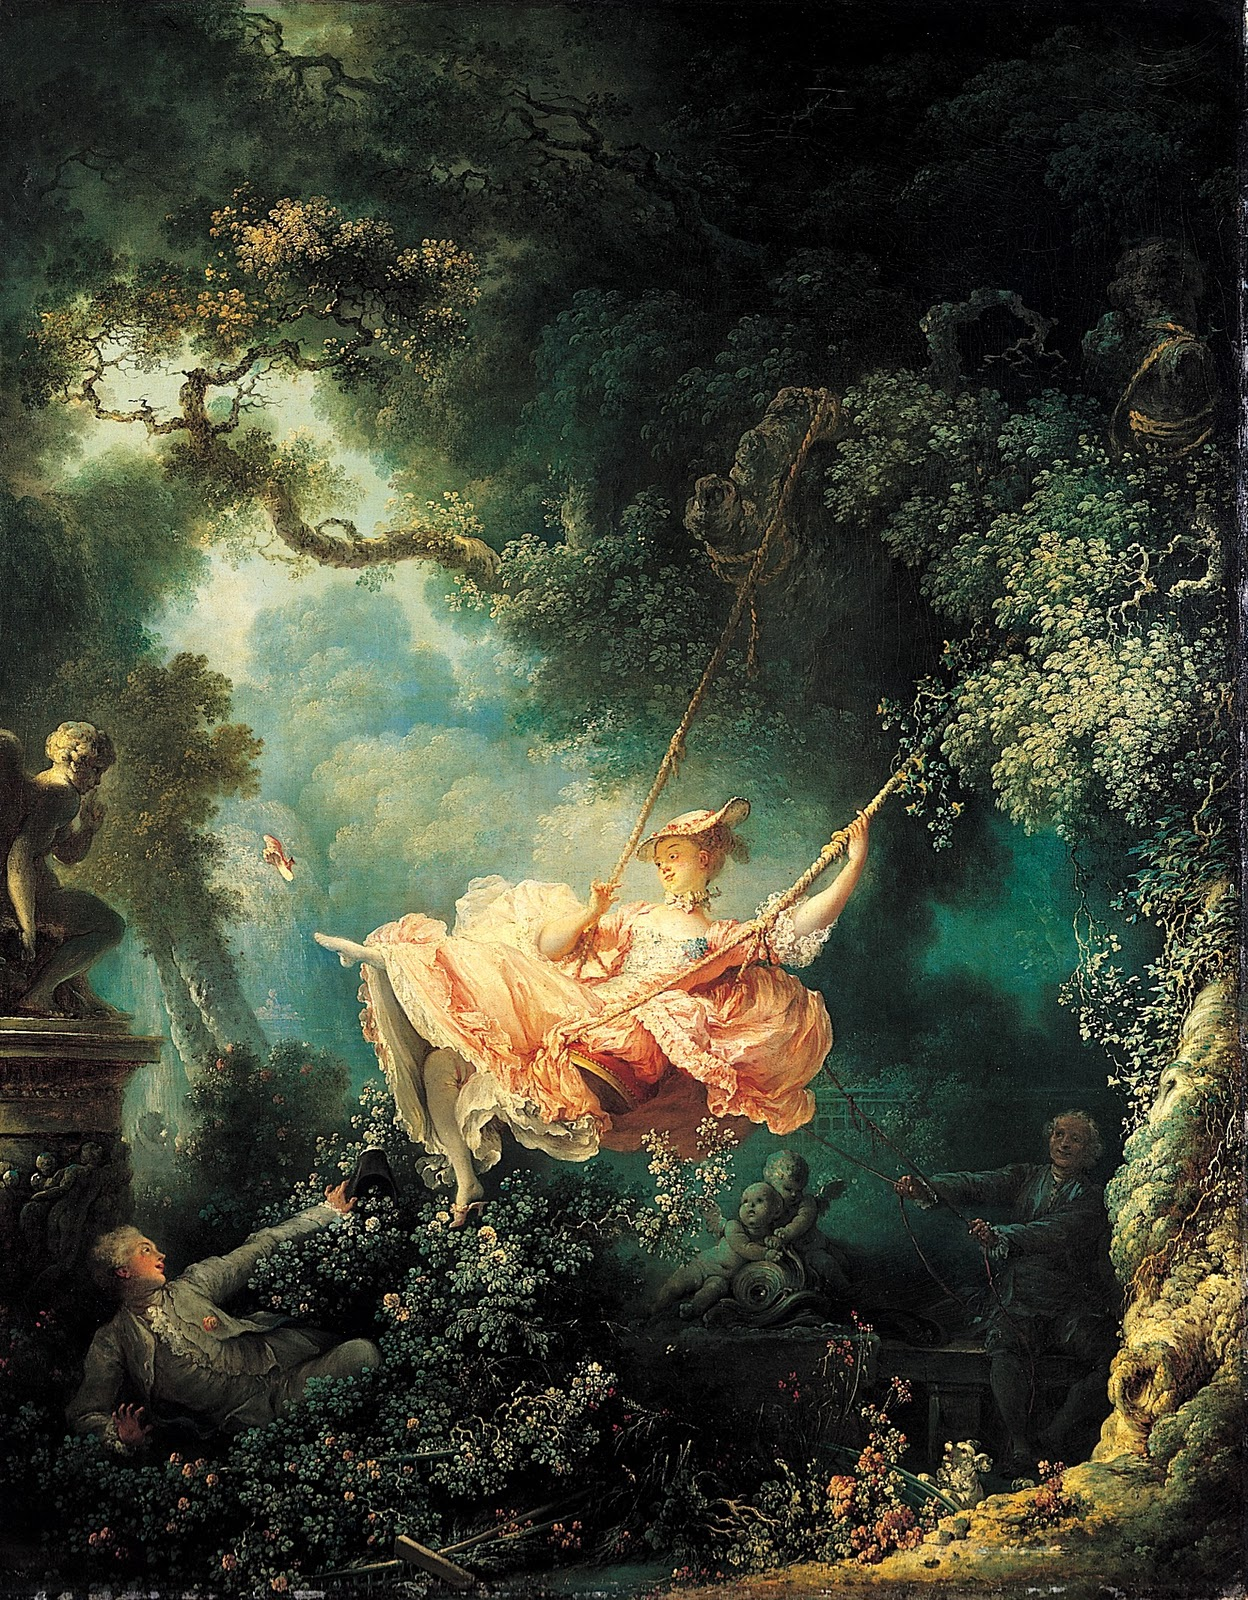
\includegraphics[width=\linewidth]{qiuqian.jpg}
  \caption[让·奥诺雷·弗拉戈纳尔:《秋千》]{让·奥诺雷·弗拉戈纳尔:《秋千》。1767年,
    布面油画。}\label{fig:qiuqian}
\end{figure}

\chapter{工作制}

\section{传统超时加班企业}

在中国,劳动密集型企业,尤其是制造业,是我们传统的超时加班重灾
区\cite{guojilaogongshijian},曾经引发社会极大关注的富士康连续跳楼事件便被认为是
因超时加班所致,仅2010一年被媒体曝光出来的就有“14连跳”。富士康为降低、杜绝
此类事件采取了一系列举措,2010年、2011年两次大幅提升工资、健全加班制,铺设大
面积防跳楼网,签订《不自杀协议》等。2011年后,就很少有相关报道了……

根据《富士康工资、工时与生产管理调研》\cite{fushikangzuixin}一文,虽然至2015年为
止,富士康工人超时加班现象仍较严重,但大量裁员现象却与之并存。“2013年媒体又
报道了富士康新一轮的变相裁员浪潮(在2013年富士康全国用工规模减少了21万),引
起工人以`跳楼'”或停工等形式的激烈反抗。”。2016年,BBC发文报道《富士康用机器
人取代了6万名工人》。

笔者实在是无法理解,十几年前乃至二十年前,是哪些人在向政府整天鼓吹2035年中
国“劳动力红利”消失,为何各部门大力推进“\textbf{无人化、少人化、智能化、信息化}”,
甚至主动要求企业升级,为何采取一系列激进的劳动力溢出政策。事实恰恰相反,我
们是严重劳动力过剩啊!我们已经有了大量的产业后备军——失业和半失业工人啊!

% 我知道“劳动力红利”除产业后备军外,还包含一个内涵的古典政治经济学“最低工
% 资”理论——工人阶级只能、也只配得到满足自己和繁衍下一代(工人阶级的再生产)
% 基本需求的工资。但过大的后备军和过低的

网友白鹤飞和澎啊湃启发了我,中国的超级城镇化进程使城市居民数量剧增的同时,更
多人口要接受各种城市公共服务收费——物业、医疗、教育、交通、治安、消防等。这
使工人最低工资水平较多增长,企业用工成本加大。

鼓吹“劳动力红利消失”并实施相关政策,继续制造更多的剩余劳动力,继续庞大本已
足够庞大的产业后备军队伍,可以打破工人工资刚性,使工人可以接受比当前最低工资
更低的工资……这一系列的超限会产生怎样恶劣后果,笔者认为无需赘述。

事实上,正是刺激劳动力红利的政策、超长工作日等,让中国人口负增长,未来可用劳
动力数量下降……

% 其实我国在2015年也启动过“马铃薯主粮化”战略。人为推进马铃薯主粮化这一战略至
% 少早在亚当·斯密《国富论》就已提出并在当时西方国家实施,意图用马铃薯主粮的综
% 合价格走低,借此减少工人工资,使最低工资可以更低……


\section{新型超时加班企业}

金融和互联网企业是二十一世纪新加班重灾区。华为在舶来词方面有个贡献,将日
本“过劳死”的概念成功传播到了中国,“加班文化”流传甚广,有很多段子。华为苏
州研究院椅子背后常备的睡袋,酷爱加班文化的日本专家入职华为两个月后愤而辞
职“你们这样是不人道的”,华为总裁任正非挽留要回北京陪妻子的副总李玉琢时
说“这样的老婆你要她干什么?”等。

说起创意,华为也一点也不比富士康《不自杀协议》差。我国于2007年6月29日颁布《劳
动合同法》,其中第十四条规定“有下列情形之一,劳动者提出或者同意续订、订立劳
动合同的,除劳动者提出订立固定期限劳动合同外,应当订立无固定期限劳动合同:
(一)劳动者在该用人单位连续工作满十年的……”。这个法案将于2008年1月1日正式
实施,华为就在2007年底要求7000余名工龄8年以上的老工人向公司递交自请辞信,作
为补偿,华为向这些老工人支付约十亿元违约金,然后再重新聘用这些“失业工人”,
工龄从零开始重新计算。数天后,2008年1月1日,工人们“自愿”为了几万到十几万的
补偿金,放弃了订立“无固定期限合同”的可能,变为了1至3年劳动合同的新工
人。“华为裁员门事件后,沃尔玛、环球、摩托罗拉等公司也先后进行了应对新法的人
力资源调整。《劳动合同法》实施前的“阵痛”似不减反增。\cite{huaweimaiduan}

2010年8月,华为“公司14级以上工人被要求`自愿'签署《成为奋斗者申请
书》……申请“华为奋斗者”有一个必备条件,需要添加“我申请成为与公司共同奋斗
的目标责任制工人,自愿放弃带薪年休假、非指令性加班费和\textbf{陪产假}”这句
话。\cite{huaweifendou}华为真是个互联网企业的好模板。

任正非在2001年有篇文章《华为的冬天》非常有名,当时国内大IT公司似乎基本没有这
种“Winter is coming”的论调,更不大认为自己可能马上狗带,他的危机意识立刻被
广大媒体、企业称赞。近20年过去,在这种强烈的危机意识下,华为仍是高奏凯歌、一
路前行。而2017年,一些年过34岁的交付工程维护人员,过40岁的研发员工和45岁的老
员工却可能迎来了真正的凛冬,要被清退掉去他处过日子了。当然,华为已经惯例辟谣
了。从此35岁陆续成为多个行业裁员和招聘的红线。

2016年8月29日起,58公司总裁兼CEO姚劲波的微博陆续被众多58公司员工、员工家属和
社会人士浏览并情绪不稳定地评论\cite{tai58},起因是58公司在不发邮件和公文的情况下
口头传播了公司新工作制度——“996工作制”,早九点上班,晚九点下班,星期六正常
上班,没有任何补贴。虽然这种工作制可能并非58公司原创,但却是由因它开始引起公
众反加班的社会影响,并且在事件后,“996工作制”并没有受到实际影响,反而成为了
不少单位一种明目张胆的制度。笔者认为,58公司“996工作制”这一事件,可以定为中
国劳动制度的一个里程碑。这标志着严重超时工作制从原来只是个别公司内部隐性文化、
不成文规定,发展至显性公司制度,并最终成为一种公开的可以被任何企业复制的社会
劳动制度。

滴滴出行于2016年底连发三篇大数据报告《2016年度加班最“狠”公司排行
榜》\cite{zuihen},涉及金融、互联网、公关、广告四个行业,包括33家公司。这33家公
司中最晚下班时间均在20点后,其中20点到21点之间下班的只有15家。四个行业相比较,
工作日时长方面金融行业较好,互联网业最差,最高加班时间是京东23点16分。周末上
班方面,金融业最差。0-5点下班返工人数方面,公关、广告公司表现突出,其中奥美广
告返工人数3080人,金宝大厦3家公司合计2102人。

\section{工作时长立法}

去看二十世纪或者当前的劳动法已经是难堪之事,那让我们粗略看下最早期的工时立法吧。

英国全行业立法是始于“1874年,R. A. Cross提出工厂方案,最终使得所有的英国工人
都享受10小时工作的权利”\cite[96]{britishworkday}。

法国一步到位,直接是全行业立法,“法国1850年9月5日的十二小时工作日法令是临时
政府1848年3月2日法令的资产阶级化的翻版;这个法令适用于一切作
坊”\cite[319]{capital}。

我们这些大体量的企业,靠着不懈的努力,向前150多年终于赶超到了英法19世纪中后期
水平,真是可歌可泣。另外,24小时工作制其实也已经来了,就是工作、睡觉、起床接
着干活,某为分公司椅子背后就挂着睡袋,随时一天24小时不离公司,祝这些企业能早
日赶超到19世纪早期劳动水平吧,就是不知道是否还需要童工呢?

结合实际来看,我国现在实行的1995年劳动法,规定的8小时工作制相比其他各国标准较
高,要求劳动时长较短,比德国、新加坡等一周60小时工作制还要少不少。在实际操作
上缺乏一些空间,可能的解决方案如弹性工作制、休息权等问题还在探讨中。希望尽快
出台相关政策。

\section{超时加班的危害和原理}
\label{sec:gzryuanli}

150多年前的《资本论》中提到的一些情况,居然仍高度适用我们的当前社会,在世界发
展方面来说这真不是一件庆幸之事。那么为何我们又重新回到150年前的工作状况?

马克思原文如下(不想看马克思原文的读者,可以略过这部分):
\begin{quotation}
  至于个人受教育的时间,发展智力的时间,履行社会职能的时间,进行社交活动的时
  间,自由运用体力和智力的时间,以至于星期日的休息时间,——这全都是废话!但
  是,资本由于无限度地盲目追逐剩余劳动,像狼一般地贪求剩余劳动,不仅突破了工
  作日的道德极限,而且突破了工作日的纯粹身体的极
  限。\cite[306]{capital}

  《1861年爱尔兰面包业委员会的报告》中提到,“委员会认为,把工作日延长到12小
  时以上,是横暴地侵犯工人的家庭生活和私人生活,这就侵犯一个男人的家庭,使他
  不能履行他作为一个儿子、兄弟、丈夫和父亲所应尽的家庭义务,以致造成道德上的
  非常不幸的后果。12小时以上的劳动会损害工人的健康,使他们早衰早死,因而造成
  工人家庭的不幸,恰好在最必要的时候,失去家长的照料和扶
  持。”\cite[292]{capital}

  工人阶级中就业部分的过度劳动,扩大了它的后备军\footnote{想在本行业入职的失业或半失
    业人}的队伍,而后者通过竞争加在就业工人身上的增大的压力,又反过来迫使就业
  工人不得不从事过度劳动和听从资本的摆布。工人阶级的一部分从事过度劳动迫使它
  的另一部分无事可做(无事可做指后备军),反过来,它的一部分无事可做迫使他的
  另一部分从事过度劳动,这成了各个资本家致富的手段,同时又按照与社会积累的增
  进相适应的规模加速了产业后备军的生产。\cite[733]{capital}

  决定工资的一般变动的,不是工人人口绝对数量的变动,而是工人阶级分为\textbf{现役军
    和后备军的比例}的变动,是过剩人口相对量的增减,是过剩人口时而被吸收、时而
  又被游离的程度。\cite[733]{capital}

  产业后备军在停滞和中等繁荣时期加压力于现役劳动军,在生产过剩和亢进时期又抑
  制现役劳动军的要求。所以,\textbf{相对过剩人口}是劳动供求规律借以运动的背景。它把这
  个规律的作用范围限制在绝对符合资本的剥削欲和统治欲的界限之
  内。”\cite[736]{capital}

  不变资本的固定部分即工厂建筑物、机器等等的规模,不管用来工作16小时,还
  是12小时,都会仍旧不变。工作日的延长并不要求在不变资本的这个最花钱的部分上
  有新的支出。此外,固定资本的价值,由此会在一个较短的周转期间系列中再生产出
  来,因而,这种资本为获得一定利润所必须预付的时间缩短了。因此,甚至在额外时
  间支付报酬,而且在一定限度内甚至比正常劳动时间支付较高报酬的情况下,工作日
  的延长都会提高利润。因此,\textbf{现代工业制度下不断增长的增加固定资本的必要性,也
  就成了唯利是图的资本家延长工作日的一个主要动力。}\cite[91]{capital3}

  资本主义生产方式按照它的矛盾的、对立的性质,还把浪费工人的生命和健康,压低
  工人的生存条件本身,看做不变资本使用上的节约,从而看做提高利润率的手
  段。\cite[101]{capital3}
\end{quotation}

以上意思是指:
\begin{enumerate}
\item 工人、职员异化成为企业身上一个微小的、易损坏和易更换替代的一个器官。不止个
  人的健康、生命受到损害,他的社交角色、儿女角色、父母角色、夫妻角色等社会角
  色也被严重削弱和抑制。在中国传统家庭人伦关系加速破裂。尤其是华为《奋斗者申
  请书》居然明目张胆“自愿”要求放弃本就不多的陪产假,真是反基本社会人伦,千
  夫可指。当然,华为始终横眉冷对,淡定得很,人家负面新闻也像富士康一样越来越
  少了,这真是进步呵!

\item 在职工人、职员的过度劳动,使当前就业人数相对于正常劳动情况下应当就业的人数
  减少了。当前未就业或者半就业工人、职员的存在又使在职工人、员工的工资报酬被
  压低。

\item 随着生产力发展,机器等固定资本的支出愈加巨大,不管其使用或不使用,都在产生
  折耗,这是生产力发展所必要的。为了事实上节约这种固定资本,就需要延长工人劳
  动时间,这就使工人超长劳动,乃至24小时劳动似乎成为一种生产力发展的必须。另
  外,如果雇佣更多工人,则需要更多数量和更大投资的固定资本,这对本已庞大的不
  变资本支出无异于雪上加霜。

\item 此外,脱离马克思文本,就实际情况来看,将工人本应得的工资分至加班费中,企业
  可以灵活运用加班政策,萧条时不加班或少加班,使工资维持在低水平,避过工资刚
  性。通过超长工作日所产生的职工数量节约,也使企业培训成本、培养成本、管理成
  本、福利保障成本、风险成本均大幅降低。
\end{enumerate}

综上,企业倾向于让员工尽量加班而非在原工作时长不变的情况下雇佣更多工人。

% 那么工人、职员为什么要加班呢?\begin{enumerate}

% \item 如富士康这类工厂,将基本工资设的较低,工人的工资财富积累常常只能在加班费中
%   来完成。不加班,不赚钱。加班了,才有钱。这是两百来年很多大工厂惯用不变的伎
%   俩。或者如华为将部分加班费融合进了工资,一些职员由此认为工资是可观的。这两
%   种情况其实都是一样的,就是企业在员工应得的工资中抽取了一部分给工人。

% \item 如华为这类企业,已在社会具有相当的名声。大众普遍认为能进华为的,肯定是有一
%   定水平的。能在华为干住的,跑到其他企业肯定是不怕累的。在一些职员看来,被压
%   榨就压榨吧,加班就加班吧,一个跳板而已。撑过现在,未来是光明的。

% \item 企业考核。不管是领导思想上的还是落在纸上的考核,都将加班量作为职员是否合格
%   的一个标准,华为有个词很有意思,叫“工作量饱满”。工作量不饱满,你就不是个
%   称职的员工。工作量饱满了,员工的个人时间,家庭时间也就别想饱满了。

% \end{enumerate}

员工作为这个微小的、易损坏的、易更换替代的螺丝钉,在工作10年左右被榨干后,甚
至只是在自己阅历增加、工龄福利增多后,便迎来自己被扫地出门的结局,他们将被年
龄更小,福利待遇更低的年轻员工所取代!超长工时所带来的利润诱惑几乎是不可阻挡
的。这便是自由!但这是资本的自由,而非人的自由!

\section{工时改革问题的民族国家与全球化困局}

重新结合实际情况立法,对工人、工会赋权,加入弹性工作制和阶梯性休假等补偿措施,
加大执法力度,主动执法,对较重违规现象进行惩罚性罚款等,这些举措理论上将能有
效解决工时严重过长的问题。

就以往传统历史经验来说,19世纪英国工作日改革经验表明,“劳动生产率和劳动强度
的变化,或者是在工作日缩短以前,或者是紧接着在工作日缩短以后发生
的”\cite[601]{capital},后来福特8小时工作制以及世界上广泛传播的劳动法
均在一定程度上证明了这点。

但现实是严酷的,我们可能无法出台实质的修正措施。中国当今所面临的正是资本语境
中,民族国家与全球化这一巨大张力困境。

所谓全球化,说穿了就是资本(尤其是金融资本)在全球高速通畅的流动。不管是中国
政府,还是美国政府,不管是工人还是大企业家在面对全球化这一庞然大物时都常是有
心乏力。中国在长期脱实向虚的城镇化改造中使工人最低工资提高较多,用于满足日益
增长的公共事业支出以及铸币税支付;而东南亚、南亚、拉美劳动市场的低廉——相当
程度上是因为当地贫困人口、童工、更贫穷国家的劳动力输入;政府的非现代化管控要
求,法律法规不健全;

所谓民族国家,则是强调本国利益,打击抵制他国相对本国的优势力量。2008年经济危
机后,世界各国看到了中国制造崛起的强势,打造各种非自由的贸易壁垒,对中国产品
出口设置各种障碍,征收各种不合理高额关税,发起各种非法反倾销反垄断诉讼、调查,
威逼利诱中国大型企业外迁;种种境况下,中国资本外逃数量恐不是少数。

民族国家并不一定和全球化相对。事实上,强国如美国,通过民族国家政策对他国的打
压,可以让本国金融资本全球化更具优势。


以富士康\cite{foxconnwiki}为例,其在巴西、匈牙利、斯洛伐克、土耳其、捷克、日本、
马来西亚、墨西哥、印度、美国均有工厂。印度方面已与富士康签订谅解备忘录,富士
康预计在5年之内投资印度50亿美元,“美国方面唐纳德·特朗普总统于2017年7月26日
宣布,富士康将在威斯康星州东南部建立一个价值100亿美元的平板电视制造工厂。威斯
康星州将每年向富士康支付高达2.5亿美元的补贴,为期十五年。这笔交易被一些人批评
为是拿取30亿美元纳税人税收资助激励富士康。威斯康星州立法机关的无党派预算办公
室的分析确定,国家纳税人将在2043年收回投资。”

外国对中国的强力抵制,并不是因为中国的意识形态与他们不同,不是中国“邪恶”,
只因我们可能变得越加强大!

这真是个困局呵。安东尼·吉登斯在《现代性的后果》一书中提出,现代性的全球扩展
趋向产生了一个“\textbf{失控的世界}“,它的出现没有人也没有政府能够全面地控制。马克思
用\textbf{怪物}来描述现代性,而吉登斯将其比作\textbf{坐在巨型汽车或”猛兽“上面}……人类的聪明
才智,在这里居然毫无用处,是我们人类自己,孕产出了这种种怪胎……

当马克思、恩格斯研究人类学时,当吉登斯希望发现未知社会模式的原始部落时,
都是这样一种绝望下的希望。虽然希望,却也绝望;虽然绝望,却也希望……

最后,用工人诗人许立志的一首诗来结束本节吧。

\poemtitle*{流水线上的兵马俑} \settowidth{\versewidth}{Than Tycho Brahe, or Erra Pater:}
\begin{verse}[\versewidth] \kaishu
  沿线站着\\
  \qquad 夏丘\ \qquad \quad 张子凤\qquad 肖朋\\ \qquad 李孝定 \qquad 唐秀猛\qquad 雷兰娇\\ \qquad 许立志 \qquad 朱正武\qquad \\ \qquad 潘霞\ \qquad \quad 苒雪梅\\这些不分昼夜的打工者 \qquad 穿戴好\\ \qquad 静电衣 \qquad 静电帽 \quad 静电鞋\\ \qquad 静电手套 \quad 静电环 \\整装待发 \quad 静候军令\\只一响铃功夫\\悉数回到秦朝
\end{verse}
\newcommand{\attrib}[1]{\nopagebreak{\raggedleft\small #1\par}} \attrib{许立志 (1990--2014)\qquad}


%%% Local Variables:
%%% mode: latex
%%% TeX-master: "../main"
%%% End:

\chapter{结合中国经济史谈一些经济概念}

\section{土地金融总结}


\section{通货膨胀税}

\textbf{通货膨胀税}是从宏观经济层次考虑的通货膨胀对货币持有者的影响,\textbf{指持有中央银
  行纸币者由于一般物价上涨(通货膨胀)所受到的损失。}

\textbf{引起通货膨胀税的原因很多,并非都是中央银行增加基础货币引起的。}例如,由于石油
价格上升等导致的成本推动型通货膨胀,由于支付技术进步导致的微观经济单位减少对
中央银行现金的需求而增加商业银行活期存款(或之前支付宝、微信钱包等金融存款方式)
导致的一般价格水平的上升。而恶性通货膨胀下,追求效用最大化的微观经济单位在恶
性通货膨胀条件下一般减少对中央银行纸币的实际需求,例如发生货币替代,对本国货
币需求减少……这样中央银行铸币税小于通货膨胀税。

\section{铸币税}

在现代经济理论中,\textbf{铸币税多指货币发行者由于在货币发行中具有一定程度的市场垄
  断权力(非完全竞争)而从货币发行中获得的利润,是一种隐形税收。}可以认为铸币
税是通货膨胀税的一个子集。

简单举一闭环例子来说,假设市场总价值变化不大,流通货币 $x$ 元。央行再发行货
币 $y$ 元,相应支出 $y$元购买商品。长期市场流通循环后,市场价值不变,却已
有 $x+y$ 元货币,通货膨胀率 $ \sfrac{y}{x}$ ,货币贬值 $\sfrac{y}{x+y}$ 。央
行通过征税、债券等方式回收货币,但货币整体已贬值,此时央行赚取的并不是超发货
币之初的 $y$ 元,而是回落到 $(1 - 货币贬值率)y$。


可以这样来简单形象理解:央行依仗垄断权利向全民强制发行\textbf{无息债券},其中的\textbf{本
  应支付却未支付的债券利息}\footnote{具体论述可见张怀清论文《人民银行铸币税的测算和
  运用 :1986--2008》}便是央行铸币暗税,\textbf{其实际收益与临期时长成正比,与周转次
  数成反比}。越先使用这张债券的部门,越受益;不参与其中投资周转的人,例如只是
储蓄或拿死工资的人蒙受全部应付未付利息的损失。

铸币税是偏向于顶富阶层的财富再分配,促使财富分化现象更加严重。在经济攀升期中
产阶级或许能收益;但即使在这种乐观时期,下层阶级也不可避免要承担最高隐形税赋!
从这种意义上来说,\textbf{铸币税是劫贫济富,这是人类从原始社会至今固有滥觞。}

以下为张怀清几篇论文的摘选:
\begin{quotation}
  不仅金属铸币、中央银行货币的发行产生铸币税,商业银行由于在存款市场具有垄断
  而获得的利润也可看作是铸币税。不仅如此,还有诸如政府债券铸币税(bond
  seigniorage)等形式的铸币税。

  随着电子通信技术的发展、金融市场的完善和金融产品的丰富,微观经济单位对中央
  银行纸币的需求呈现相对减少趋势,不仅商业银行类金融机构正在发行可在一定程度
  上替代中央银行纸币的货币,其他金融机构发行的金融产品也在很大程度上替代中央
  银行纸币和商业银行负债。

  国际货币基金组织(IMF)曾于1998年分别考察了欧洲和北美等21个发达国家以及亚洲和
  拉丁美洲等79个发展中国家,得出结论: 1980–1995年期间,发展中国家铸币税收
  占GDP的比重平均在1.4\%–3\%之间,大大高于发达国家平均在0.64\%左右的水平。而
  中国在同一时期,铸币税占GDP的比重平均为6.52\%( Massonetal, 1998),除了少数
  几个发生过超级通货膨胀的国家之外,已是世界上最高的国家之一。

  不同的学者利用不同的方法得到的估计有所差异,谢平(1994)按照基础货币增量的算
  法,得出我国1986--1993年之间,政府每年得到的货币发行收入占国内生产总值的比
  重平均为5.4\%;易纲(1996)得出1978--1992年真实铸币收入平均占GNP的3\%左右;周
  立(2003)认为1984--1996年期间的大部分年份的真实铸币收入
  占GDP的5\%--7\%,1993年和1996年达到8.5\%。但无论是哪一种算法得出的结果都远
  远高于发达国家的平均水平0.64\%,也在很大程度上超出发展中国家的平均水
  平1.4\%--3\%。
\end{quotation}

另外本国货币如能作为国际货币使用,自然也可向其他国家收取铸币税。人民币国际
化还任重道远,较多采用货币互换方式,能收取的国际铸币税较少。根据人行《2023 年
人民币国际化报告》
\begin{quotation}
  2023 年一季度末,人民币国际化综合指数为 3.26,同比上升 10.2%。
  同期,美元、欧元、英镑、日元等主要国际货币国际化指数分别
  为 57.68、22.27、7.66 和 5.48。

  2022 年,人民币跨境收付金额合计为 42.1 万亿元,同比增长15.1\%。其中,实
  收 20.5 万亿元,同比增长 10.9\%;实付 21.6 万亿元,同比增长 19.5\%,\textbf{收付
    比为 1:1}。
\end{quotation}

\improve[inline]{读者如有意,可加入商业银行存贷铸币税、互联网金融公司铸币税
  等论述。}

\section{超发货币和居民消费价格指数CPI}

根据《黄金时代:应对超现实风险的真实解决方
案》\cite{piepenburg2022gold},自1983年起,以购房是投资而非消费为由,不再将\textbf{房
  价}计入消费者物价指数CPI,取而代之的是增长速度远低于房价的% 主要居所租
% 金(rent of primary residence)和
\textbf{业主等价租金}(owners’ equivalent rent, OER,简单理解就是如果房主将房子出
租所能获得的租金),CPI被严重低估。以中国为例,中国重点50城租售比自2019年后始
终在1:600以下,且租售偏离程度持续扩大,也就是租房50余年才可收回房价。


此外《黄金时代》还写到:
\begin{quotation}
  美联储多年来一直公开撒谎,淡化真正的通货膨胀……\textbf{CPI表是一个公开的骗局},
  这允许美国劳工统计局(BLS),因此也允许美联储,以他们认为合适的方
  式 "报告 "通货膨胀——至少目前是这样。

  如果使用20世纪80年代美联储CPI通胀加权方法衡量今日,那么美国在2021年的CPI通
  胀率将接近15\%,而不是报告的6\%多。

  美联储简单调整了其衡量通货膨胀的CPI尺度,有效淡化了住房、医疗保健和教育方面
  的成本上升,以衡量消费者价格通货膨胀……简言之,美联储不喜欢用旧的CPI尺度来
  衡量通货膨胀,所以他们简单地用\textbf{2+2=2}的CPI来代替它。

  同样,美联储为了保持其\textbf{由欠条驱动(即债务驱动)的“复苏”假象},别无选择,
  只能\textbf{发明一个可控的(即较低的)CPI通货膨胀率},以便使美国国债在与通货膨胀
  相比较时,看起来对其他债务驱动买家更有适度的吸引力。


  \textbf{保持债券和债务市场活力的唯一方法是通过“过度印刷”来摧毁国家的基础货币。简
  而言之,畸形膨胀的市场可能在利率抑制的刀锋下生存,但货币,嗯......他们死在
  同一把剑下。}

  当然,\textbf{这是在吃你的蛋糕,但不是在吃它}……

  为了进一步欺骗人民,这个“魔术”背后的所谓专家想出了MMT(即现代货币理论,主
  张\textbf{财政赤字货币化}。)这个舒缓的概念,以使这种腐败的东西看起来更符合逻辑,
  更正式,甚至更聪明。对政策魔术师来说,这种语义上的技巧并不新鲜。当他们需要
  欺骗人民时,他们会巧妙地从字母表中抽出令人平静的字母,发明一些听起来很有学
  术性、有效和健全的政策名称,比如MMT或QE(\textbf{量化宽松})。但是,这两个现在常
  见的政策名称都不过是指\textbf{凭空伪造货币,这是一种公开的荒谬}。

  \textbf{量化宽松只是制造并扩大了有记录以来最大的风险资产泡沫和贫富差距。}

  \textbf{今天全球的特点是不顾一切地扩大广义货币供应,以解决不可持续且史无前例的债
    务水平。}这种扭曲而一贯的政策错误,导致了历史上最大的风险资产泡沫……正如
  历史所提醒的,所有的泡沫都会破灭。


  当股票\textbf{在投机性政策的支持下不合逻辑地上涨时,尽管其政策制定者有信誉的“逻
    辑”,但事实上没有逻辑,随之而来的极端纸面财富获得了永久甚至稳定的幻觉。}但
  是,正如我们和赫斯曼当时所警告的那样,今天更是如此,投资者很快就会集体陷入
  一种错觉,认为他们今天投资组合中的数万亿美元代表着明天的持久购买力。换句话
  说,“合乎逻辑”的投资者总是忽略了一个历史上被证实的事实,即\textbf{一旦上升的东
    西崩溃,大部分的财富最终会蒸发掉。}简而言之,风险资产从未变得更有风险。例
  如,截至目前,全球金融资产的价值(股票、债券和房地产)是520万亿美元,是全
  球84万亿美元GDP的\textbf{6.2倍}。

  考虑到持续增长和怪诞的债务水平,决策者实际上别无选择,只能膨胀他们的债务。
  作为聪明的小狐狸,公共政策制定者当然会尽一切努力,故意允许\textbf{通货膨胀(以偿
    还债务)},同时控制收益率曲线来\textbf{人为抑制利率},\textbf{从而抑制债务成本}。同样,
  这种绝望的利率压制对于爬进2020年代的“破产”主权国家来说是必须的。再说一遍:
  他们别无选择……\textbf{摆脱债务的唯一方法是让通胀率高于利率——差距越大,摆脱债
    务的速度就越快。}

  考虑到当前大于300万亿美元的全球债务水平,如果允许\textbf{利率自然上升}(即在真正
  的资本主义中),政府债务的利息支出将在几秒钟内大幅超过GDP的50\%,全球债务方
  和所谓的“经济复苏”将立即以戏剧性的方式结束。

  如果 CPI 通胀率被准确报告,那么公开虚假的美国国债实际收益率将为负值,美联储
  通过给这种收益率涂上口红,可以继续依靠更多债务、更“有吸引力”的欠条和更多
  的欺骗为生。这种隐蔽的通胀欺诈行为让美国能够有效地延长和掩盖历史上史无前例
  的债务狂潮,而美国信贷市场就像一个名副其实的科学怪人一样前进——它已经死了,
  但仍然在所谓“无通胀”但永久的货币创造的氧气下前进。但即便是弗兰肯斯坦最终
  也会死去。
\end{quotation}

就今日世界大国强国实践,尤其是美国而言,超发货币、寅吃卯粮已是长期传统,\textbf{报
  表上的CPI指数意图掩盖的是真实通货膨胀、货币发行机构所收取的铸币税;超发货币
  实则是金融虚拟资本(包括房地产,房地产真实属性是金融)对其他赛道人民的盘剥。
  收入不平等加剧、财富极度分化就这样静悄悄地来到了现代社会。}

其实现代国家往往都习以为常施用各种“真实数据烟雾弹”……数据可以是真实的,但却是在
各种别有用心统计方法下的真实数据。


\section{GDP、GNI和分配正义}

据国家统计局,

\begin{quotation}
  国内生产总值(Gross Domestic Product,GDP),是指一个国家或地区所有常住单位在
  一定时期内生产活动的全部最终成果,等于所有常住单位创造的增加值之和。可
  见,GDP强调国内生产,体现的是增加值的生产创造。


  国民总收入(Gross National Income,GNI),是指一个国家或地区所有常住单位在一
  定时期内收入初次分配的最终结果,等于所有常住单位的初次分配收入之和。

  GNI,即在GDP的基础上,扣除外国在本国的资本和劳务收入,加上本国从国外获得的
  资本和劳务收入。
\end{quotation}

不管GDP还是GNI,都是以加总方式来衡量国家经济。当代所有国际几乎都热衷于用这两
种方式来描述国内经济状况。这两个指标都无法说明、甚至不想说明分配不均、贫富差
距、社会福利这类问题。资本主义发端之初,新古典(自由主义)经济学家们便惯于使
用国民经济这一加总说法。

如亚当·斯密《国富论》:
\begin{quotation}
  劳动获得宽裕的报酬,不仅是一国财富\textbf{不断增加}的必然结果,同时也是一国财
  富\textbf{不断增加}的自然症候。另一方面,贫穷的劳动阶级生活捉襟见肘,是一国财
  富\textbf{停滞}的自然症候,而该阶级人民濒临饿死,是一国财富\textbf{迅速萎缩}的自然症候。
\end{quotation}


国民经济的发展(GDP或GNI等) \neq 大部分国民的经济发展 \neq 国民的幸福。

恩格斯和马克思分别写到:
\begin{quotation}
  这一事实无非是表明:劳动国民财富这个用语是由于自由主义经济学家努力进行概括
  才产生的。只要私有制存在一天,这个用语便没有任何意义。英国人的“国民财
  富”很多,他们却是世界上最穷的民族……在这种科学看来,社会关系只是为了私有
  制而存在。\pagescite[][60]{maenwen1}


  我们且从当前的国民经济的事实出发。工人生产的财富越多,他的生产的影响和规模
  越大,他就越贫穷。工人创造的商品越多,他就越变成廉价的商品。\textbf{物的世界的增
    值同人的世界的贬值成正比。}劳动生产的不仅是商品,它还生产作为商品的劳动自
  身和工人,而且是按它一般生产商品的比例生产的。\pagescite[][156]{maenwen1}
\end{quotation}

张文喜探讨了《所有制与所有权正义:马克思与“亚当·斯密问题”》\cite{ZXYJ201404002}:
\footnote{\url{https://www.dswxyjy.org.cn/n1/2019/0617/c427160-31162202.html}}:
\begin{quotation}
  在对斯密等人的评述中,马克思明确指出存在私有财产和工人需要的悖论,认为市民
  式的自私自利能够保证与公共利益先天和谐,这是一种幻象。斯密的自然自由原理与
  利益和谐的自由市场学说注定满足不了任何一个阶级的要求:\textbf{工人和资本家同样苦
  恼,没有财产的工人是为他的生存而苦恼,“资本家则是为他的死钱财的赢利而苦
    恼”}(《马克思恩格斯全集》第3卷,第227页);因而,“既然按照斯密的意见,大
  多数人遭受痛苦的社会是不幸福的,\textbf{社会的最富裕状态会造成大多数人遭受这种痛
    苦},而且国民经济学(总之,私人利益的社会)是要导致这种最富裕状态,那么国民
  经济学的目的也就是社会的不幸”。(同上,第230页)

  \textbf{生产资料私有制给特定的阶级带来的具体结果,在本质上绝不是像斯密所讲的共同富
  裕,而是两极分化。}
\end{quotation}


1993年,中国正式采用GDP作为经济表现的指标,从此开始了追求GDP增速的历史。
回到亚当·斯密,中国持续发展可以“先富带动后富”,并且确实使国人生活水平普遍
大幅提高。但中国如何应对“财富停滞”时“贫困的劳动阶级生活捉襟见肘”,又如何应对
经济危机、财富迅速萎缩时的“濒临饿死”呢?

四十多年来,中国刺激经济持续增长多是以\textbf{大规模超发货币}为主要手段,用基建、房地产等
作为通货膨胀蓄水池,甚至在某种意义上使基建、房地产本身成为超发的货币。这一政策核
心至少自上世纪70年代末的“洋跃进”便已出现,只是那时候还没有房地产的加入。

凯恩斯主义是短期应用经济学,且要求针对经济萧条和上升期适时调整;它对于长期无
力,长期应用必然持续集聚毒性。每一次的负债经济增长都必然使将来市场出清、结算
埋单时期更加残酷惨痛。

为缓解危机,除非我们能将危机转嫁至他国或者参加战争。问题是,太多发达国家也是
这样想的——一方面担忧已在世界资本市场长袖善舞的中国经济危机导致世界经济危机,
引发种种问题;另一方面希望啃蚀世界最大市场之中国的血肉,将自身危机转嫁至中
国。我们太愿意以债养债、寅吃卯粮了,到了一种非理性的程度。

另外我们的贫富分化已在狂热追求GDP的过程中持续加大.

\begin{quotation}
  北京大学以全国25个省市160个区县的14960个家庭为基线样本所得的《中国民生发展
  报告\textbf{2015}》显示,\textbf{最富有的1\%的家庭占有近1/3的全国财产,而底端25\%的家庭
    拥有的财产总量只占1\%左右。}\cite{dajueqi}
\end{quotation}

2023年贝恩公司与招商银行联合发布《2023中国私人财富报告》,提到
\begin{quotation}
  2022 年,中国个人可投资资产总规模达 278 万亿人民币,2020-2022 年年均复合增
  速为 7\%;到 2024 年底,可投资资产总规模预计将突破 300 万亿关口。

  2022 年,可投资资产在 1,000 万人民币以上的中国高净值人群数量达 316 万人,人
  均持有可投资资产约3,183 万人民币,共持有可投资资产 101 万亿人民
  币,2020-2022 年年均复合增速为 10\%;预计未来两年,中国高净值人群数量和持有
  的可投资资产规模将以约 11\% 和 12\% 的复合增速继续增长。
\end{quotation}
也就是说在中国,\textbf{0.22\%的人口(高净值人群)占据了总可投资资产的31.96\%,}高
净值人群可投资资产增速倍数于GDP增速,也意味着财富分化趋势更一步加大。

相比贝恩和招行报告,瑞士信贷和瑞士银行发布的《2023年世界财富报告》相对乐观
些,但只是相对。中国的百万美元富翁数量已占世界11\%,仅次于美国的38\%。
\begin{quotation}
  自2000年以来,\textbf{中国的财富不平等现象大幅上升}。2000年\textbf{财富基尼系数为59.5},稳
  步上升,\textbf{2016年达到71.7}。2000年,前1\%人群的财富份额
  为20.7\%,2021年为30.5\%,2022年上升至31.4\%。

  迄今为止美国\textbf{百万美元}富翁人数最多,为2270万,占世界总数的\textbf{38.2\%}。这遥
  遥领先于排名第二的中国,中国占全球百万富翁总数的\textbf{10.5\%}。在本世纪初,日本
  的百万富翁数量与美国竞争,之后日本的地位一直在稳步下降,于2014年被中国超
  越,2022年仅占百万富翁的4.6\%,首次排在第四位,仅次于法国(4.8\%),并受到
  德国(4.4\%)和英国(4.3\%)的挑战。
\end{quotation}

\begin{table}[hbt!]
\centering
\resizebox{\textwidth}{!}{%
\begin{tabular}{@{}llllllllllllllll@{}}
\toprule
\multicolumn{1}{c}{} & \multicolumn{7}{c}{\textbf{基尼系数}}              &  & \multicolumn{7}{c}{\textbf{1\%最富有的人财富占比}}      \\
                     & 2000 & 2005 & 2010 & 2015 & 2020 & 2021 & 2022 &  & 2000 & 2005 & 2010 & 2015 & 2020 & 2021 & 2022 \\ \midrule
巴西                   & 84.5 & 82.7 & 82.1 & 88.7 & 88.9 & 89.2 & 88.4 &  & 44.2 & 45   & 40.2 & 48.7 & 49.5 & 49.3 & 48.4 \\
美国                   & 80.6 & 81.1 & 84.1 & 84.9 & 85   & 85   & 83   &  & 32.9 & 32.8 & 33.4 & 34.8 & 35.3 & 35.1 & 34.2 \\
印度                   & 74.6 & 80.9 & 82.1 & 83.3 & 82.3 & 82.3 & 82.6 &  & 33.2 & 41.9 & 41.4 & 42.3 & 40.5 & 40.6 & 41   \\
德国                   & 81.2 & 82.7 & 77.4 & 79.2 & 77.9 & 78.8 & 76.9 &  & 29.1 & 30.4 & 25.7 & 32.1 & 29.2 & 31.7 & 30   \\
加拿大                  & 74.9 & 73.3 & 71.7 & 71.8 & 71.8 & 72.6 & 72.3 &  & 29.1 & 25.9 & 22.4 & 23.3 & 23.6 & 25   & 24.3 \\
\textbf{中国大陆} &
  \textbf{59.5} &
  \textbf{63.8} &
  \textbf{70} &
  \textbf{71.2} &
  \textbf{70.5} &
  \textbf{70.1} &
  \textbf{70.7} &
  \textbf{} &
  \textbf{20.7} &
  \textbf{24.2} &
  \textbf{31.5} &
  \textbf{31.7} &
  \textbf{30.8} &
  \textbf{30.5} &
  \textbf{31.1} \\
台湾                   & 64.7 & 67.8 & 72.6 & 70.5 & 70.7 & 70.7 & 70.5 &  & 24.3 & 23.6 & 29.8 & 26.9 & 27.3 & 26.6 & 26.4 \\
法国                   & 69.7 & 67   & 69.8 & 69.9 & 70   & 70.2 & 70.3 &  & 25.5 & 21   & 21   & 22.3 & 21.9 & 22.3 & 21.2 \\
英国                   & 70.5 & 67.6 & 69.1 & 73   & 71.7 & 70.6 & 70.1 &  & 22.1 & 20.6 & 23.6 & 25   & 23.1 & 21.1 & 20.7 \\
西班牙                  & 65.5 & 62.2 & 61.4 & 69.5 & 69.1 & 69.1 & 68.3 &  & 24.1 & 18.7 & 18.5 & 24.1 & 22.7 & 23.1 & 22.4 \\
韩国                   & 69.7 & 70.1 & 74.7 & 72.4 & 67.7 & 68.2 & 67.9 &  & 21.3 & 21.8 & 26   & 26.9 & 23.4 & 24   & 23.1 \\
意大利                  & 60.4 & 59.4 & 63.1 & 66.9 & 66.4 & 67.2 & 67.8 &  & 22   & 18.2 & 17.4 & 22.6 & 21.9 & 23.3 & 23.1 \\
澳大利亚                 & 63.7 & 63.1 & 63   & 64.9 & 65.5 & 66.2 & 66.3 &  & 20.5 & 20   & 19.2 & 20.5 & 20.6 & 21.8 & 21.7 \\
日本                   & 64.5 & 63.1 & 62.5 & 63.6 & 64.4 & 64.7 & 64.8 &  & 20.4 & 18.8 & 16.7 & 18.2 & 18.1 & 18.7 & 18.8 \\ \bottomrule
\end{tabular}
}
\caption{财富不平等趋势}
\capsource{来源:瑞士信贷和瑞士银行《2023年世界财富报告》}
\label{tab:gini}
\end{table}

上一节已经提过,超发货币可以采用直接超发,量化宽松或赤字货币化等形式。这些形
式均是为大金融资本服务的财富持续分化武器!

无论是新官不理旧账的官僚考核制度,或是被债务绑架选择以债养债,都只像是表象而
非本质,没有触及核心本质。本质是金融精英和权力贵族的结合体?希望读者或者他人
能够进一步阐述。

\todo[inline]{我国热衷超发货币、追求GDP的深层动因、逻辑,或许是金融资本精英加
  权力贵族对于资本增殖的需求?考虑列入土地金融总结部分。}


\part{国际政经}
\chapter{罗斯福新政与凯恩斯主义}

% http://ias.cssn.cn/cbw/mgyjjj/1991/dyq_119068/201506/t20150616_2688427.shtml
% https://www.sohu.com/a/197986540_567589
% http://old.civillaw.com.cn/Article/default.asp?id=27826
% https://www.aisixiang.com/data/110057.html

1929年美国爆发严重经济危机,经济大萧条,并扩散至世界,主张自由放任市场调节完
善性的经济学彻底倒台。1933年当选的美国罗斯福总统发布一系列政策,试图依靠国家宏观
调控能力缓解经济周期中下行期的萧条影响,史称罗斯福新政。

不少人(包括经济学家)认为罗斯福新政主要是受英国经济学家约翰·梅纳德·凯恩斯
影响;也有不少人对此反驳,认为罗斯福受凯恩斯的影响较小。争议综述可参考刘绪
贻。

笔者认同刘绪贻\cite{roosevelt}、张小鲁\cite{bijiao202002}、张世
明\cite{JJFX200100010}等人观点,\textbf{罗斯福新政与凯恩斯关系并不大,凯恩斯指导罗斯福
  新政是个“童话”。}单是两人行动时间节点就可以提供不少作证。另外早期制度经济
学派代表凡勃伦、康芒斯对于新政的影响力也远比凯恩斯大得多。

根据布鲁和格兰特《经济思想史》摘抄如下:
\begin{quotation}
  康芒斯的第一本著作《财富的分配》(1893)并没有获得充分认同。批评家认为,这是
  康芒斯为其\textbf{社会主义思想}确立科学基础的一次令人不满尝试。然而,康芒斯并不是
  一个试图改变私人财产和自由企业社会结构的革命家。他认为,\textbf{资本主义的本质可
    以并且应当保持完整无缺,但是,经济秩序的运转规则需要变革,以消除自由放任
    经济体的明显缺陷。}在威斯康星大学,他的观点获得了州长拉·弗利特(La
  Follette)的支持。

  被一些人称作\textbf{威斯康星学派}(Wisconsin school)的经济学方法,主要是在\textbf{康芒斯}的
  影响下在威斯康星大学得到发展。\textbf{这种方法支撑了美国的非正统经济理论,发动了
    改变美国经济结构与功能的改革}。

  威斯康星州政府广泛利用威斯康星大学教职工充当新思想的智囊团、法律的起草者以
  及指定委员会的成员。

  体现在罗斯福新政社会立法中的很多思想来自于威斯康星州,这一点很少有人怀疑。毫
  无疑问,1932 年,很多在麦迪逊接受培养的经济学家和其他人都搬到了华盛顿特区。
\end{quotation}

其实凯恩斯也了解过马克思,根据《经济思想史》,凯恩斯在《通论》第一稿中有对马
克思关于资本循环的论述和注解,第二稿中删除。另外凯恩斯学生中也有一些马克思主
义者。
\begin{quotation}
  凯恩斯的学生莫里斯·多布还是一位研究生时,曾在凯恩斯的房间里读到一篇论述马克
  思与剑桥政治经济学俱乐部的论文。多布回忆道,凯恩斯很赞许这篇论文,因为“他
  年轻时在一定程度上喜欢非正统思想”。
\end{quotation}

缘何凭空造就力挽狂澜美国于大萧条的“凯恩斯童话”,笔者不明就里,只敢妄加揣测:
难道是因为凯恩斯作为英国政府高级代表参加1944年的布雷顿森林会议,制定了当代国
际金融体系,并与美国财政部官员哈里·德克斯特·怀特(Harry Dexter White)一起
创立了国际货币基金组织(IMF)和世界银行(World Bank)?或者为了\textbf{增加货币超发
  的伪合法性以实现进一步财富分化}?其实“所谓罗斯福新政采用的是凯恩斯式的扩张
性财政和货币政策,从而挽救了美国经济。\textbf{数据证明这并非事
  实。}”\cite{bijiao202002}。


对罗斯福新政和凯恩斯主义的论述有助于理解国家干预政策,有助于构建一条资本主义
发展史链条。


\section{罗斯福新政}

本节大量参考王小鲁《美国大萧条与新政再思考》\cite{bijiao202002}。罗斯福新政主要
还是应用经济,是应对当时大萧条的实用政策,主要包括以下内容。

\begin{enumerate}
\item 保障劳动者的基本权利,制定最低工资标准、实行8小时工作制、禁止使用童工。这
  些劳工保障措施于1935年被最高法院宣布违宪,随国家复兴署的裁撤而终止,直
  到1938年美国国会通过了新的《公平劳动标准法案》后才重新得以实行。

\item 大幅度增加政府的社会保障和救济等福利支出,建立了劳动者的养老保险和失业保险
  制度,逐步替代了临时性社会救助的功能。

\item 改善收入分配状况,减少过大贫富差距。如提高\textbf{个人所得税}的累进率,征
  收了累进的\textbf{遗产税}和\textbf{财产税}。据王小鲁:
  \begin{quotation}
    在这一变化中减少的主要是个人财产收入的份额,\textbf{对企业利润份额没有影响,因
      此企业家的积极性也受到了保护}……到1950年没有太大变化,其中财产收入份额
    进一步下降,公司利润份额上升了。
\end{quotation}

\item 规范工农业生产和产品价格,防止过度竞争,促进价格止跌回升。

\item 新政未使用凯恩斯主义要求的扩大政府借债和支出政策,大搞基建。

  据王小鲁,当时已经货币严重超发,甚至可能正是货币超发才引起美国经济大萧条,
  罗斯福自然不可能依据凯恩斯的请求继续超发货币。
  \begin{quotation}
    大萧条之前美国已确实经历了长期的货币宽松。但并非如罗斯巴德所说主要发生
    在20世纪20年代,而是持续了更久。更宽松的时期是在20世纪10年代……
    1917-1919年,美国参加一战,政府以\textbf{巨额赤字}支持了军事支出扩张,而该支出的大
    部分都是通过借债和货币发行筹集的。这解释了20世纪10年代货币快速扩张的原因

    (20年代)货币事实上超量供应。而且这是在20世纪10年代货币严重超发基础上的
    继续。\textbf{长期货币扩张最后导致股市崩盘、引发萧条的说法是有充分根据的。}
  \end{quotation}

  据列宁,金融和垄断资本发动的一战使自由资本主义从垄断阶段走向国家垄断资本主
  义。笔者认为,这也标志着所谓自由资本主义的破产。虽然“事实上,没有任何干预
  的“纯粹”市场经济在历史上从来没有存在过”,以后也不会出现。
  \begin{quotation}
    \textbf{世界托拉斯和银行资本为争夺世界市场的统治权而引起的世界大战}, 使物质财富遭
    到巨大破坏, 使生产力消耗殆尽, 使军事工业蓬勃发展, 以致绝对必需的、 最低限
    度的消费品和生产资料的生产无法进行。

    战前在最发达的先进国家中无疑已经具备的社会主义革命的客观前提(笔者注,这
    里列宁还是过于乐观了),由于战争而更加成熟,并且继续在异常迅速地成熟。中
    小经济更加迅速地遭到排挤和破产。资本的积聚和国际化正在大大地加强。\textbf{垄断
      资本主义正在向国家垄断资本主义转变},由于情势所迫,许多国家实行\textbf{生产和分
    配的社会调节},其中有些国家进而采取\textbf{普遍劳动义务制}。\pagescite[][441]{lenin29}
  \end{quotation}

  据克里斯·哈曼:
  \begin{quotation}
    正如希法亭、布哈林和列宁所指出的,当“自由市场资本主义”开始让位于“垄断
    资本主义”及其产物帝国主义时,\textbf{经济“自由主义” 已在实践中被替代了。国家
      干预被认为是为资本主义生产提供基础设施所必需的}(铁路在德国长期以来就是
    国有化的,在英国,保守党政府将电网和航空公司国有化)。后来的战时国民经济
    组织——最初出现在德国和日本,后来又出现在英国和美国——表明\textbf{国家干预可
      以为收益率和积累的复苏提供基础}。
  \end{quotation}

  据王小鲁,罗斯福也没有大搞基建:
  \begin{quotation}
    除了田纳西工程,新政期间政府还投资了3万多个公共工程项目,小型项目居
    多……大多采取以工代赈的方式。这些项目对改善基础设施条件、减少失业、减贫、
    环境治理和带动经济增长发挥了一定作用。但政府投资并不是新政的核心。
  \end{quotation}

\end{enumerate}

\section{凯恩斯主义}

虽然大萧条救市和凯恩斯关系不大,但较多经济学家认为凯恩斯于1936年发表的《就业、
利息和货币通论》创建了现代宏观经济学。

凯恩斯经济学\cite{jahan2014keynesian}的立足点是,\textbf{总需求}(以家庭、企业和政府
的\textbf{总支出}来衡量,包括消费、投资、政府购买和净出口,凯恩斯没有对支出进行细
分。)是经济中最重要的驱动力。\textbf{自由市场没有导致充分就业的自我平衡机制}---“长期
来看,我们都死了”。失业和经济危机的原因是\textbf{有效需求不足}。

经济周期中的下行期,随着总体需求的持续下降,消费者信心不足减少\textbf{消费支出},进
而企业减少\textbf{投资支出}。\textbf{政府支出的积极干预}便有助于缓和经济周期的繁荣上升和
萧条下行期幅度,并且是必要的。

具体举措是政府针对经济周期情况\textbf{适时干预}:在需求测(总支出)下降时,对\textbf{劳动
  密集型基础设施项目}进行\textbf{赤字支出和降低利率},增加社会福利,以刺激就业和稳
定工资,修复消费和生产循环。在需求测增长充足时,\textbf{提高税收以冷却经济并防止通货
膨胀}。


二战后世界各国政府常常应用凯恩斯主义,加强对经济生活的全面干预,直
至20世纪60年代末、70年代初,西方世界出现经济停滞或衰退、企业倒闭、工人失业和
通货膨胀并存的现象——“\textbf{滞胀}”,凯恩斯主义受到其他学派巨大挑战,面临前所未
有危机。此后有一些学者对凯恩斯主义进行不同改造。

一个有意思却未必正确的观点:\textbf{凯恩斯主义是劫小康、济大贫、修缮大权贵}。

它是应用政策经济学,而非学院理论经济学。它是\textbf{短期}需求管理政策,漠视长期经济周
期,\textbf{坚持长期使用将成为越来越毒的毒药},在未来市场出清、结算总账时带来更加巨大
的灾难,包括但不限于“滞胀”;如同任何经济学说一样,它不能消除资本主义经济固
有的基本矛盾。

\section{从垄断资本主义到国家垄断资本主义}

在马恩看来,国家是阶级矛盾不可调和的产物,是统治阶级的统治工具,用于“缓和经
济利益互相冲突的阶级,\textbf{不致在无谓的斗争中把自己和社会消灭}”。资本主义以降,
市民社会是国家的基础,市民社会的阶级张力与矛盾制约和决定了国家,而不是相反。
国家不是社会的主宰物,恰恰相反,国家是社会发展的\textbf{产物}。

关于市民社会中的统治阶级,可能是政府内阁;更可能是“统治阶级不统治”,藏在幕
后的国内外金融大佬。经济学家们五花八门、各圆其说、常彼此矛盾的妙计锦囊,只被
用作统治阶级的政策支持武器,哪个趁手拿哪个,加以改造,用完即弃。分析现实经济
政策,切忌用XX经济思想标签这些武器套取,要像福尔摩斯一样关注背后的获利群体。

笔者认可刘绪贻的论断:
\begin{quotation}
  \textbf{罗斯福新政与凯恩斯主义同是垄断资本主义向国家垄断资本主义转变过程的典型产物。}
\end{quotation}

不少国人听到国家垄断资本主义,就会想起当时的苏联,其实核心一致,只是欧美的国
家垄断程度不如苏联的更高些罢了,可叫\textbf{社会自由主义}或者左翼自由主义等。
\begin{quotation}
  社会自由主义(Social liberalism,也可称为Newliberalism),与John
  Ruggie在1982年提出的\textbf{镶嵌型自由主义、嵌入式自由主义}(Embedded liberalism)
  相通。其代言人为\textbf{凯恩斯、罗尔斯和德沃金等,主张国家干预经济生活,可通过加
    大政府支出、投资来解决失业和消费不足经济危机,重视社会福利。}它允许社会和
  经济的不平等,但主张\textbf{政治自由权的平等优于经济自由权的平等},要求国家给予民
  众关怀和尊重。\cite{newneo}
\end{quotation}

它,资本主义,进化了!


% 我国铸币税个别参考文献
% 1995年禁止中央财政直接向人民币透支:

% 1995年《中国人民银行法》公布以前,财政部可以向人民银行借款和透支,用于弥补中
% 央财政赤字和解决专项支出。《中国人民银行法》关于“中国人民银行不得对政府财政
% 透支,不得直接认购、包销国债和其他政府债券”的规定出台后,中央财政不能再从人
% 民银行借款。同时《预算法》规定政府财政赤字只能通过发行国债来弥补。自2003年初
% 以来,为对冲因外汇储备增长过快而导致基础货币投放过多的影响,人民银行在加大公
% 开市场回购操作力度的同时,大量发行央行票据,回笼货币,以保证货币供应适度增长。
% 随着人民银行持有的债券大量到期,其公开市场操作工具不足的问题日益突出,实施货
% 币政策的操作压力不断加大。截至2003年7月末,广义货币和狭义货币供应量同比分别增
% 长20.7\%和20\%,大大高于年初确定的调控指标,货币超经济供应现象逐渐显现。为解
% 决人民银行公开市场操作工具不足问题,确保现阶段货币供应与经济发展相适应,有必
% 要将中央财政这部分历史借款转换为标准的、可交易的国债。2006年,吴汉洪和崔
% 永[4]对我国铸币税的研究进行了小部份综述。

% 参考文献
% [1] 张怀清. 论中央银行铸币税和通货膨胀税的关系[J]. 南方金融, 2007(10): 28–30.
% [2] 张健华, 张怀清. 人民银行铸币税的测算和运用:1986–2008[J]. 经济研究, 2009(07): 79–90.
% [3] 张怀清. 商业银行铸币税研究[J]. 金融发展研究, 2008(04): 12–15.
% [4] 吴汉洪, 崔永. 中国的铸币税与通货膨胀:1952–2004[J]. 经济研究, 2006(9): 27–38.

% 在时任总理温家宝(1953-)的领导下,中国党/国家对2008年全球金融危机的反应实际
% 上是提振“总需求”,政府采取措施通过“量化宽松”计划刺激经济,其中包括对全国
% 基础设施的广泛投资,其中包括4万亿元人民币(5860亿美元)的刺激计划。 被描述
% 为“凯恩斯博士的中国病人”(见《经济学人》2008:1)。然而,问题在于储蓄和消费
% 之间的“结构性失衡”是否可以得到解决(Fang and Gang 2009:149)。“乘数效
% 应”可能起效缓慢,提振内需可能说起来容易做起来难。中国的收入不平等程度很高,
% 官方的基尼系数为0.47,但实际上可能要高得多,可能超过0.60(见Warner
% 2013:177)

% ,“供给侧改革”成为引领经济政策的新动向,它主张通过促进分工深化来提升全要素
% 生产率进而提高潜在产出水平。显然,“供给侧管理”的理论基础与其说是新古典经济
% 学(包括凯恩斯主义经济学),不如说是古典经济学和马克思主义经济学。

\chapter{新自由主义札记}
\label{chap:neoliber}

\section{新自由主义的概念}
\label{sec:neoliberalism}


中国语境中常说的“\textbf{新自由主义}”实为Neoliberalism,即“\textbf{新古典自由主义}”,
它不同于前一章结尾所说的社会自由主义Newliberalism。维基英文版
对Neoliberalism的解释如下:
\begin{quotation}
  新古典自由主义,主要是指19世纪初与\textbf{自由放任的经济自由主义}相关的思想\footnote{古
    典自由主义(Classical liberalism)中的\textbf{经济自由部分}}在20世纪的复苏。这
  些想法包括\textbf{经济自由化}的一系列政策,如私有化,财政紧缩,放松管制,自由贸易
  和减少政府支出,以增加私营部门在经济和社会中的作用。这些\textbf{以市场为基础}的思
  想及其所激发的政策促成了从战后的凯恩斯主义(1945--1980)到新古典自由主义的
  范式转变。

  学者现在倾向于将其与朝圣山学派的经济学家弗里德里希·哈耶克、米尔顿·弗里德
  曼和詹姆斯·M·布坎南,以及玛格丽特·撒切尔,罗纳德·里根和艾伦·格林斯潘等
  政治家和政策制定者联系起来。
\end{quotation}

新自由主义理论内部并非铁板一块,充斥着各种学派,如\textbf{现代货币学派、理性预期学
  派、供给学派}等等,这些学派彼此之间也存矛盾、异议,各国政府的新自由主义实践
依时间、国情等的不同,对这些理论的侧重均有不同\cite{neoxuepai},也有一些早期的热
情拥护者和参与者如今也都\textbf{转向批判立场}。\improve[inline]{好像哈耶克也有转向和反
  思,最好能提供这方面资料。}


\section{哈维对新自由主义实践的批判}

本节内容主要参考大卫·哈维的《新自由主义简史》。

新自由主义理论口号所宣称的实则是一种\textbf{乌托邦}。它宣称市场放任的\textbf{经济自由}远比一
切其他方面的自由(尤其是政治自由)更为重要,认为\textbf{经济自由是其它自由的唯一基
础}。并且其理论和真实实践(对新自由主义的应用)存在着相反面。

新自由主义真实的\textbf{实践内容}主要有:
\begin{enumerate}
\item 美国为首的发达国家向其它弱国推行新自由主义,倡导经济自由,\textbf{实则是使新自由
    化的弱国更易被强国资本全球化组织获取高利。}在收割过程中,以强国国力作为背
  书,\textbf{实现强国的超额利润和绝对主导地位,造成弱国的社会悲剧深渊}。还有强国对
  弱国放贷,往往以自由化为前提且要求债权人的至上权力和债务人的无限责任,其实
  即使是古典经济学、凯恩斯主义等也反对债权人的无风险。美国也可以依托美元
  的“世界货币”地位,直接在全球化中抽取高额利润。

  正如斯蒂格利茨的讽刺“这是多么古怪的世界啊,\textbf{反倒是贫穷的国家在补助最富裕
    的国家}\cite[75]{davidneoliber}。笔者觉得斯蒂格利茨有点过于惊乍了,
  世界任何组织不总是在向下劫贫济富么……


\item 在放任的市场经济自由内部,本身也是\textbf{大资本(尤其是金融资本)的各方面霸权体
    现,而非经济自由和平等}。如经济精英对弱势者的剥削;垄断或寡头的形成;市民
  隐性或显性的税赋形成的政府投入成为精英阶层生财资本和工具;快速私有化过程中
  国有、集体资本被精英阶层严重折价收购从而使私人资本在收购结束时就已获取超量
  巨额利润;金融资本远远超越生产资本占据强势地位,一部分工业资本也纷纷实现金融
  化。

  即使是凯恩斯也鄙视食利者,提出“\textbf{食利者的安乐死}”,如今却是\textbf{食利者的迷醉
    狂欢}。

\item 新自由主义确实产生了一些其它自由,如择业自由、言论自由等。但这种附带自由很
  是有限,并且
  \begin{quotation}
    如卡尔·波兰尼所说“这些自由在很大程度是‘\textbf{市场经济的副产品,这同一种经
      济也要为那些恶的自由负责}’”。

    就不好的自由方面,波兰尼列出的有“\textbf{剥削他人的自由,或获得超额利润而不对
      社会做出相应贡献的自由,阻止技术发明用于公益事业的自由,或发国难财的自
      由}”。

    \textbf{自由的理念由此“堕落为仅仅是对自由企业的鼓吹}”,这意味着“那些其收入、
    闲暇和安全都高枕无忧的人拥有完全的自由,而\textbf{人民大众仅拥有微薄的自由},尽
    管他们徒劳地试图利用自己的民主权利来获得某种保护,以免遭那些有钱人的权力
    的侵害”。但是——事情往往如此——如果“\textbf{没有权力和压制的社会是不存在的,
      强力不发挥作用的世界也是不存在的}”,那么维持这种自由主义乌托邦前景的唯
    一办法就是靠\textbf{强力、暴力和独裁}。在波兰尼看来,自由主义或新自由主义的乌托邦
    论调注定会为权威主义甚或十足的法西斯主义所
    挫。 \cite[38-39]{davidneoliber}
  \end{quotation}

\item 金融和跨国集团等“实力自由派”,凭借新自由主义意识形态,并非要求国家无所作
  为,而是试图\textbf{让国家全力为己服务},尤其是在难见市场效益的公共事务上的巨额投
  入——往往是巨额赤字,与法律法规的的倾斜。

  新自由主义赖以实现的并非如它宣称“否定国家干预”。恰恰相反,\textbf{它必须大力借
    助于国家的强力,甚至暴力和独裁,还有凯恩斯主义的赤字投入}。国家在此的作用
  并非是为了民众自由或普惠,而是被作为\textbf{有利于上层阶级的财富和收入再分配的工
    具},成为\textbf{上层精英获利手段},国家沦为企业资本和上层阶级的“\textbf{守夜人}”。
  新自由主义意识形态,借此成为最强且普遍的规训手段,为强大资本主义、现代性理
  性代言和背书。

  我国社科院的“新自由主义研究”课题组认为:
  \begin{quotation}
    该课题组将“新自由主义”的主要观点归纳和概括为以下三点:在经济理论方面大力
    宣扬\textbf{“三化”(自由化、私有化、市场化)},在政治理论方面特别强调和坚
    持\textbf{“三否定”(否定公有制、否定社会主义、否定国家干预)},在战略和政策方
    面\textbf{“极力鼓吹以超级大国为主导的全球经济、政治、文化的一体化,即全球资本
      主义化}”。\cite{newneo}
  \end{quotation}
  社科院这个课题组似乎只注意到了新自由主义经济理论层面内容,没有注意其实践本
  质,没有看到其要求国家干预并为资本精英和权力贵族牟利这一点,没有意识到政治权
  力沦为资本权力附庸?笔者对此失望。

\item \textbf{一切成为商品,人的肉体、精神以及权利也均被作为经济商品对待,无助于
    实现物质价值的便被认为是无价值的。}即使对资本精英来说,消费主义的盛行也造成表
  面满足、内心空洞、身份焦虑等。\cite[179]{davidneoliber}

\item \textbf{社会、集体团结的意愿缺失},必然使人试图从他处寻得(很有限的)满足。
  催生\textbf{黑社会、边缘群落、非政府组织、以及宗教团体}等。
\end{enumerate}

\begin{quotation}
  总体而言,新自由主义化\textbf{无法刺激经济增长或提高人民生活}。第二,从上层阶级角
  度出发,新自由主义\textbf{进程而非其理论}确实是巨大的成功:它要么\textbf{重建了统治精英
    的阶级力量}(如美国和某种程度的英国),要么\textbf{为资产阶级形成创造了条
    件}(如中国、印度、俄罗斯等等)。……不管出现什么问题(不平等、低薪、失业
  等),都是因为缺乏竞争力,或因为个人、文化、政治上的缺陷,以上论述宣称,在
  一个\textbf{社会达尔文主义}的新自由主义世界里,只有适者才应该也能够生
  存。\cite[164]{davidneoliber}
\end{quotation}

\section[新自由主义的实质]{新自由主义的实质——哈曼对哈维的批判}

克里斯·哈曼\cite{chrisharmanneo1} \cite{chrisharmanneo2}和大卫·哈维都认为在新自由
主义国家的实践过程中均出现了与它所宣称的\textbf{背离}。在美国、中国等国的新自由主义
实践中,均采用了新自由主义表面反对的\textbf{凯恩斯主义的国家干预}为经济发展提供保
障,例如\textbf{政府大规模财政赤字、不良银行债券资助基础设施建设和固定资本投资}等。
其他被灌输并实行较为彻底新自由主义化的落后国家,则被美国等国\textbf{利用资本全球化
  进行掠夺和积累}。

% 哈维认为寻求自由的新自由主义却要求国家干预是其\textbf{悖论},这一
% 悖论所产生的真正原因是“\textbf{新自由主义的主要实质成就不是生产财富和收入,而是对
%   财富和收入进行分配}\cite[165-166]{davidneoliber}”,“\textbf{旨在重建资本
%   积累的条件并恢复经济精英(资产阶级)的权
%   力}\cite[19-20]{davidneoliber}”。
哈曼以更为激进和传统的马克思主义视角对哈维提出了批评。哈曼认为“新自由主
义”这一意识形态提法具有\textbf{模糊性},它\textbf{弱化了国家支出}在新自由主义实践中的地
位,相比注重就业和福利的凯恩斯主义,\textbf{新自由主义要求的国家投入更高};\textbf{抬高了
  积累过程中“暴力”的地位,忽视了资本在阶级生产方面的强大理性和连续性——资
  本主义自始自终在原始积累(包括斯大林农业集体化政策);过于强调了工业资本和
  金融资本的对立,忽略了工业资本也加快了金融化;弱化了工人阶级的强大力量。}

\begin{quotation}
  “新自由主义”实际上并不是对今日资本运行的精确描述。我们没有面临向\textbf{自由市
    场资本主义}的回归,这种资本主义在一个世纪以前就\textbf{完结}了。我们面临的是这
  样一个体系,它尝试着在全球范围内\textbf{重建}它体系的各个单元来解决它自身的问题,
  这些单元出现于20世纪的进程中,马克思主义者称之为“\textbf{垄断资本主义}”、“\textbf{国
    家垄断资本主义}”或“\textbf{国家资本主义}”。\textbf{国家继续扮演重要角色},\textbf{想方设
    法为垄断资本提供便利或进行管理}……即使\textbf{生产的国际化}使得这样做比战后几
  十年更加困难。

  对马克思来说,原始积累不仅仅是早期资本家通过抢劫积累财富。它主要是\textbf{从农民
    手中掠夺土地,然后迫使他们寻找雇佣工人的工作。}它的特殊性不在于剥削阶级以
  武力增加他们的财富(这在各种阶级社会中都发生过)。至关重要的是,它允许发展
  一种特定的资本主义方式来扩大这种财富,通过创造一个“自由”工人阶级,他们别
  无选择,只能将他们的劳动力出卖给现在控制生产资料的人。

  这种形式的“原始”积累一直持续到今天。埃及的老地主、巴西的农业资本家、中国
  的共产党老板和印度新近建立起来的资本主义农民,都在不断地试图夺取当地农民的
  土地,在他们成功的地方,\textbf{一个新的无产阶级就诞生了。但哈维错误地认为这只是
    最近几十年的特征。}
\end{quotation}


似乎可以从哈曼的论述中得出这样一个结论:

从日不落英国到吸收了他国人力物力财力的美国初期:资本主义自由的胜利;从俾斯麦
时期的普鲁士 \footnote{对工人阶级实行鞭子加甜面包”政策:一方面解散工人组织,查禁进
  步报纸和刊物,另一方面增加医疗保险法、工伤事故保险法、残疾和老年保险法
  等。\cite[75]{zhuzhaiwenti}}到国家资本初步发达的二十世纪初期德国\footnote{1890年德国
  社会民主党占据议会27.2\%的席位,1912年提高到34.8\%。},再到一战、罗斯福新政、
苏联、上世纪60年代末:古典自由资本主义衰退,国家垄断资本主义步步兴起;从70年
代美国至今:资本对国家力量的利用,国家日益成为服从于、服务于资本逻辑的“守夜
人”,不停公共债务、财政赤字、超发货币……虽然资本主义危机避无可避,但它却是
总体向上发展的?!

只是,我的朋友,代价呢?未来呢?

以上只是笔者初步猜想,毕竟似乎有些神枪手谬误……欢迎交流和批判。


\section[联合国债务与人权独立专家报告]{联合国债务与人权问题独立专家报告摘抄}

布雷顿森林机构和发达国家常为向其它国家贷款或减债而附加\textbf{自由化、私有化、全球
  化}的条件,联合国多项机构和议题均涉及对此的强烈批判。因相关议题和文档过多,
笔者以较为随机的方式选择了\textbf{外债与人权独立专家的年度报告}作为切入点,以求管中
窥豹。

独立专家人选不同,其倾向、水平也有不同,希望大家能够批判辩证来看。笔者个人认
为,Fantu Cheru的报告有理有据,水平极高,可作重点研究。

联合国人权高级专员办事处官网链接:\url{https://www.ohchr.org/CH/Pages/Home.aspx}。

联合国外债问题独立专家年度报告链接:\url{https://www.ohchr.org/CH/Issues/Development/IEDebt/Pages/AnnualReports.aspx}


\textbf{人权事务高级专员办事处}(联合国人权高专办)是联合国\textbf{主要的人权实体}。联合
国大会赋予了高级专员及其办事处一个独特任务,即:促进和保护所有人的所有权利。

\textbf{联合国人权委员会}根据《联合国宪章》于1946年在联合国经济社会理事会第一次会议
上成立。2006年3月15日,联合国大会以170票支持、4票反对和3票弃权多数通过成
立\textbf{联合国人权理事会},取代联合国人权委员会。人权理事会是由47个成员国组成的政
府间机构,负责在全球范围内加强促进和保护人权的工作。\textbf{美国于2018年退出}人权理
事会。

人权理事会是\textbf{独立于}人权高专办的实体。这种划分源于联合国大会的分别授权。尽管
如此,人权高专办为人权理事会会议提供实质性的支持,并跟进理事会所作出的评议。

\textbf{联合国外债与人权问题独立专家}的职能是就国家外债、国际金融对人权\footnote{尤其是经
  济、社会和文化权利}的影响问题开展分析研究,进行国家访问任务,致力于与政府、
联合国、非政府行为者和其他利益相关者合作。

在人权委员会对充分享有人权的诸多议题中,\textbf{中国}几乎一直投赞成票,\textbf{切实表现出
  负责任的大国姿态},英法意德韩日等常为自身资本利益投反对票。

\begin{enumerate}
\item 1999年,独立专家Fantu Cheru向人权委员会提交报告E/CN.4/1999/50。报告
  认为,\textbf{货币基金组织、世界银行和七国集团(简称G7)的政府官员是第三世界负
    债发展的根源。}它们在债务国家未能及时还款时,一般要求债务国家以加紧实
  施\textbf{结构调整方案(全球化和自由化)}为条件,重订还款期限。它们的结构调整方
  案使债务国家陷入更为严重的经济和社会危机,指责货币基金组织和世界银行
  为“\textbf{新自由派反革命}”,“债务危机被用来作为打开第三世界市场,剥夺政府在
  国家发展中作用的方便借口”。

\item 2000年,特别报告员Figueredo、Fanto Cheru,和独立专家Reenaldo向人权委员会提
  交报告E/CN.4/2000/51。报告开篇写到:
  \begin{quotation}
    将近20年来,国际金融机构和债务国、债券国政府乐于一场自欺欺人的游戏,从远距离操
    纵第三世界的经济,强行让毫无力量的第三世界国家接受不得人心的经济政策,却自认
    是最终将使那些国家走上繁荣的道路和摆脱债务的宏观经济调整苦药。
  \end{quotation}

  布雷顿森林机构,如世界银行和货币基金组织,在\textbf{全球联盟压力下}于1996年秋天批
  准了\textbf{重债穷国计划}(the Heavily Indebted Poor Countries,缩写
  为HIPC)。HIPC要求债务国首先“必须在世界货币基金组织的强化结构调整方案
  (ESAF)下完成六年结构调整,然后要满足一些额外条件才能减免债务”。1999年春,
  货币基金组织和世界银行在\textbf{国际大庆2000运动的政治压力下}对HIPC作检讨。
  \begin{quotation}
    \textbf{简单地说,HIPC/ESAF是国际货币基金组织和世界银行通过后门继续控制穷国和债
      务国国家发展政策的一种手段。}
  \end{quotation}

\item 2001年,独立专家Fantu Cheru向人权委员会提交报告E/CN.4/2001/56。报告认真分
  析了非洲九国向IMF和世界银行提交的临时减贫战略文件
  (I--PRSP)。Cheru认可IMF和世界银行此举有积极的一面,但也提出一些批评,
  如I-RPSP是\textbf{根据捐助方设计的模版编制},“谈不上国家所有权的真实可靠
  性”,“仍导致一种把社会和人的发展以及公平方面的关注问题放在次于财政方面考
  虑因素地位的局面”。希望IMF和世界银行能进一步改进。

  报告指出IMF和世界银行很大程度上服务于主要股东,即\textbf{七国集团(G7)的利
    益},“在这方面,也不可忽视\textbf{美国财政部}的作用”。批评G7不作为。

\item 2003年,独立专家Bernards Mudho向人权委员会提交报告E/CN.4/2003/10。报
  告中强调了一些成功的案例,也指出
  \begin{quotation}
    \textbf{非政府组织}认为,大量证据表明\textbf{结构调整战略是失败的},因为没有解决国际
    金融机构经济政策在世界各地造成的日益严重的贫困和不平等。……\textbf{重债穷国倡
      议、结构调整战略和减贫扶助信贷不仅不会成功,而且将使穷人的生活更加艰难},
    因为其目的是紧缩预算,实行的政策将缩小经济生产能力,减少可行和可持续性就
    业。

    \textbf{借款人和债权人}应该对重债穷国和最不发达国家目前无法持续的外债\textbf{承担共同
      责任。}
  \end{quotation}

\item 2004年,独立专家Bernards Mudho向人权委员会提交报告E/CN.4/2004/47。报
  告指出,
  \begin{quotation}
    独立专家赞同世界银行业务评价部回顾的主要结论,即《重债穷国倡议》是一项有益
    但有限的手段,必须在债务国和国际社会需要对于整体的发展筹资方法作出更广泛承诺
    的范围内加以考虑。
  \end{quotation}

\item 2005年,独立专家Bernards Mudho向人权委员会提交报告E/CN.4/2005/42。报告延续
  上年宗旨,对IMF和世界银行总体持肯定态度。

\item 2006年,独立专家Bernards Mudho向人权委员会提交报告E/CN.4/2006/46。报告中提
  请人权委员会延缓“\textbf{八国集团(G8,俄罗斯为新加入国)倡议}”截止日期的进步性。
  \begin{quotation}
    由八国集团(G8,俄罗斯为新加入国)在 2005 年夏天提出的“\textbf{多边债务减免倡
      议}”\textbf{预测}IMF、世界银行国际开发协会(开发协会)和非洲开发基金(非发基
    金)会 100\%减免世界上负债最沉重穷国的债务,以帮助这些国家实现千年发展目
    标……

    但是首先,\textbf{只有成功完成重债穷国倡议的国家}(迄今只有 19 个)\textbf{才符合资
      格}。其次,只有三个多边开发银行参加债务减免倡议,使得特别是拉丁美洲和亚
    洲国家仍然承担沉重的债务。

    独立专家\textbf{遗憾}地指出,世界银行下设的国际开发协会将2003年定为取消合格债务
    的“\textbf{截止日期}”,这一举措不符合G8的最初提议,并将导致债务减免大量损失。
    他请开发协会重新考虑其决定。
  \end{quotation}

\item 2007年,独立专家Bernards Mudho向人权理事会提交报告A/HRC/4/10。报告中
  \begin{quotation}
    遗憾的是,近二十年期间,贸易自由化在实施上往往\textbf{操之过急},并且\textbf{顺序安排
      不当}。有时更易为\textbf{经济教条}所左右,而不是就对之可能产生的\textbf{经济和社会
      影响}作出有事实根据的分析。
  \end{quotation}


\item 2008年,新任独立专家Cephas Lumina向联合国大会提交报告,A/63/289。报告
  中Cephas Lumina概述了自己的执政方针,着重指出\textbf{人权法的首要地位和人权的中心
    地位}。
  \begin{quotation}
    可以辩称,根据国际法,国家的人权义务凌驾于许多其他种类法律义务之上,因此,
    国家,以及作为国际法主题的国际组织,采取的所有行动都应与国际人权法一致。
  \end{quotation}

\item 2009年,独立专家Cephas Lumina向人权理事会提交报告A/HRC/11/10。报告中关于债
  务减免所附条件的脚注是
  \begin{quotation}
    例如,根据Eurodad最近一项研究,\textbf{国际货币基金每一笔低收入贷款通常附加13项条件;
    大多数条件要求实行私有化和自由论,对借款国家的穷人造成严重后果。}
\end{quotation}

另一个脚注提到世界银行一份报告指出
\begin{quotation}
  过去几十年里包括\textbf{世界银行}在内向贫穷国家提出的大多数政策忠告都强调参加\textbf{全
    球经济}的优势。\textbf{然而全球市场远非公平,其运作管理规则对发展中国家造成比例
    偏高的不利影响。}这些规则是经过复杂的谈判进程所取的结果,然而在这其中发展
  中国家却\textbf{没有什么发言权}”(加重强调)。世界银行,2006年世界发展报告:公平与
  发展(纽约:牛津大学出版社,2006年)。
\end{quotation}

此外
\begin{quotation}
  过高的债务偿还以及对债务减免和新贷款的附加条件通常\textbf{限制公共开支}(甚至有
  损于向教育和保健等基本公共服务提供资金),\textbf{促进经济自由化(包括国营企业私
    有化,解除投资管理并引进公共服务使用费)},以及\textbf{优先考虑债务偿还}而忽视
  满足基本需求,这些不仅使\textbf{贫穷恶化},而且对发展中国家的\textbf{教育和保
    健}造成尤其严重影响。
  \end{quotation}

\item 2009年,独立专家Cephas Lumina向联合国大会提交报告A/64/289。报告中Lumina援
  引多方国家、组织、个人对“\textbf{非法债务}”的定义,希望依据公平、公正、持久、人
  权原则等,建立有权确立债务非法性的机构,建立负责任融资框架等。
  \begin{quotation}
    \textbf{债务人和债权人共同承担责任的原则是平等的全球金融系统的核心。}如同在《蒙特雷共
    识》中强调的,“债务人和债权人必须共同负责防止出现和解决债务不可持续的情况。”
  \end{quotation}

\item 2010年,独立专家Cephas Lumina向联合国大会提交报告A/65/260。基金组织和世界
  银行对贷款和债务的减免机制常常附加\textbf{私有化}以及贸易和金融部门所需的\textbf{贸易自由
    化}政策。报告中认为这些贸易自由化使债务加剧和不可持续,并对人权,尤其是经
  济、社会和文化权利及发展权造成不良影响和灾难性后果。

\item 2010年,独立专家Cephas Lumina向人权理事会提交报告A/HRC/14/21。报告中
  定义了“\textbf{秃鹫基金}”的概念。秃鹫基金侵蚀了贫困穷国从《重债穷国倡议》和
  《多边债务减免倡议》(尽管存在种种缺陷)中获得的收益。呼吁各国立法限制秃鹫基金,
  其中美国、英国、比利时已经或者正在执行相关遏制法律。笔者注:实际上,秃鹫基
  金在金融领域发展迅猛。
  \begin{quotation}
    “秃鹫基金”一词用于描述私人商业实体通过购买、转让或其他交易
    形式,获得违约或不良债务,有时是实际的法庭裁决,以期获得高回报。从主权债务的
    角度来说,秃鹫基金(或如它们通常自称的“问题债务基金”)一般会在二级市场
    上\textbf{以远低于其面值的价格}获得穷国(其中很多是重债穷国)的\textbf{违约主权
      债务},然后企图通过\textbf{诉讼、扣押财产或施加政治压力}寻求获得\textbf{债
      务全额面值连带利息、罚金和法律费用}的偿付。根据非洲开发银行(非行),秃鹫基金
    的平均回收率为其投资的\textbf{3--20倍},相当于300--2000\%的利润率。非行把这种回
    收率描述为“可能是问题债务市场中\textbf{最高}的”。目前,既\textbf{没有法律限
      制}这种基金可通过诉讼获得的利息或利润总额,也没有管理框架要求披露这种基金
    的\textbf{购债成本}。

    秃鹫基金诉讼案件通常都在发达国家的法院上提出。这里可能是秃鹫基金的注册地或贷
    款协定中指定的管辖区。多数诉讼案件都是在\textbf{美利坚合众国、大不列颠及北爱
      尔兰联合王国和法国的法院}提起的,这些地方被视为“\textbf{有利于债权人
      的}”辖区。

    世界银行和基金组织承认商业债权人提起的诉讼“阻碍了向重债穷国提供完全的债务减免”。
  \end{quotation}

\item 2011年,独立专家Cephas Lumina向人权理事会提交报告A/66/271。报告中介绍
  了\textbf{出口信贷机构对国家可持续发展和人权造成的不利影响}。

  \begin{quotation}
    “\textbf{出口信贷}”一词系指一种保险、担保或融资安排,它使出口资本货物和服务的
    购买人能推迟一段时间付款(包括通常为两年以下的短期信贷,通常为两至五年的中
    期信贷,以及通常为五年以上的长期信贷)。出口信贷是出口信贷机构提供的主要贷
    款。

    \textbf{出口信贷机构}是公共实体,向母国的私营公司提供政府担保或补贴的贷款、担
    保、信贷和保险,以支助\textbf{出口和对外投资},尤其是对发展中国家和新兴经济体
    的出口和投资。大多数发达国家至少有一个出口信贷机构,通常是其政府的官方或准官
    方机构。

    出口信贷和投资保险机构一般称为出口信贷机构。这些机构作为一个整体,是为外
    国企业参与发展中国家\textbf{大规模工业和基础设施项目、尤其是采掘业部门项目提供
    公共融资的主要来源。}

  出口信贷机构\textbf{以低于私人市场的利率、保险费和手续费提供融资},且这些机构对提
  供支助提出的经济条件很低,只需有限度地遵守(或根本不用遵守)环境、社会和透明
  度标准,使金融交易得以更容易、更快捷地进行,但其风险也更高。然而,对发展中
  国家的借款人而言,出口信贷机构担保的贷款的利率仍\textbf{高于}开发银行或机构等其他
  官方来源提供的许多贷款的利率。

    大多数出口信贷机构则完全没有促进发展的任务。这些机构的\textbf{唯一目标}就是促
    进\textbf{本国的出口或对外投资}。
  \end{quotation}

\item 2012年,独立专家Cephas Lumina向联合国大会提交报告A/67/304。报告中介
  绍了国际金融机构在向借款国提供贷款、赠款和债务减免时所附加的经济改革条件,对借
  款国妇女权利造成的影响。如\textbf{削减政府开支,进行公共部门改革、公共服务私有
    化和贸易自由化}。
  \begin{quotation}
    IMF和世界银行估计,重债穷国的偿债金额占国民收入的百分比已从 2000 年的 4\%以上
    跌至2009 年的 1\%,而减贫支出占国民收入的百分比已从 2000 年的 7\%增至 2009 年
    的9\%。
  \end{quotation}

  报告中肯定了债务减免对穷国的一些积极作用,“然而,必须强调,债务减免通常并
  不降低重债穷国的脆弱性,因为许多国家仍然严重依赖外国贷款和投资。”

\item 2013年,独立专家Cephas Lumina向人权理事会提交报告A/HRC/23/37。

  \begin{quotation}
    虽然现行国际债务减免举措减轻了重债穷国的债务负担(从账面来看),但这些举措未能
    处理致使低收入国家的\textbf{债务无法持续}的根本原因,这些原因包括不公正的全球
    贸易条件,生产和出口基础狭窄,容易遭受外来冲击(包括国际资金量的减少),以及不
    负责任的放款等。实际上,这些举措侧重把债务降至债权人认为“\textbf{可持续}”的
    水平,这样做隐含的意思是:问题在于接受债务减免的国家在债务管理上欠谨慎而且治
    理不善。\textbf{债权人在举措中发挥主导作用,这是与共同责任原则相抵触的。}同时,
    与举措相关的附加条件损害了债务国的主权,在某些情形中妨碍了债务减免的减贫目标
    的实现。
  \end{quotation}

\item \label{item:2012report} 2013年,独立专家Cephas Lumina向联合国大会提交报告 A/68/542。报告主要根据
  《联合国千年发展目标差距工作队2012年报告》,总结\textbf{千年发展目标8与实际进展的
    差距},希望建立更为强大的发展框架。报告中提出千年目标8实际进展过程中的不足和缺陷有:
  \begin{quotation}
    \textbf{发达国家持续的农业补贴也继续对发展中国家的农业贸易和生产产生不利影
      响。}2011年,经合组织国家的农业补贴增加到国内生产总值的 0.95\%。虽
    然\textbf{发达国家农业补贴一天为 10 亿美元},许多贫穷发展中国家无力补贴其农业,
    导致其产品价格较高,农民的贫困加剧和生活水平下降。发达国家还\textbf{对进口的制
      成品和加工产品征收高额税,使得发展中国家无法赚取更多收入,并使他们只限
      于原材料出口。}贸易谈判多哈回合停滞不前使得问题进一步复杂化。

    \textbf{二十国承诺抵制所有保护主义措施},并纠正任何在应对全球金融危机中所采取
    的保护主义措施。但2008世界贸易自危机开始以来\textbf{只废除了一小部分已经实施
      的贸易限制}。迄今实施的贸易限制已影响到将近 3\%的世界贸易。遭到\textbf{保护
      主义措施}的影响。

    如独立专家在提交人权理事会的报告(A/HRC/23/37)中所指出,\textbf{债务减免的直接
      财政影响难以衡量,债务减免与减贫支出增加之间的因果关系也难以确定}。

    债务减免机制已经\textbf{完全为债权人所主导},过度侧重于纠正被视为是受援国方面
    不慎重的债务管理,没有债务解决问题的根本原因,包括不公平的贸易条件、不负责任
    的贷款和国际金融机构不当的政策规定。
   \end{quotation}

 \item 2013年,独立专家Cephas Lumina向人权理事会提交报告A/HRC/25/52,说明不把非
   法资金归还来源国对享受人权的负面影响。
  \begin{quotation}
    “\textbf{非法资金}”一词泛指腐败、贿赂、贪污、逃税和其他犯罪行为的收益。
  \end{quotation}

\item 2014年,独立专家Cephas Lumina向人权理事会提交报告A/HRC/25/50。报告
  中Lumina总结了自己2008--2014任期内的工作。
  \begin{quotation}
    人权理事会的一些成员\textbf{没有为外债和人权这一任务提供支助,尤其是欧洲联盟和
      美利坚合众国。}
  \end{quotation}


\item 2015年,独立专家Juan Pablo Bohoslavsky向人权理事会提交报告A/HRC/28/60。报
  告主要涉及\textbf{非法资金流动}问题。
  \begin{quotation}
    根据全球金融诚信组织的最新\textbf{估计},发展中国家在2012年因非法资金外流损失
    了\textbf{9912亿美元},比2011年再增加1.8\%。2003年以来,非法资金外流实际每年增
    加9.4\%。通过将这些数字与发展中国家收到的官方发展援助比较即可表明这种资源
    流失的规模。2012年的官方发展援助为897亿美元,这意味着,2012年每支出\textbf{1美
      元的发展援助},就有超过\textbf{10美元}以\textbf{非法资金外流}的形式逃离发展中国家。
    根据全球金融诚信组织的资料,\textbf{过去十年官方发展援助和外国直接投资加在一起
      也抵不上发展中国家的非法资金外流。}

    根据保护记者委员会的资料,截至2014年12月31日,在1992年以来全球被谋杀
    的725记者中,有208人或29\%报道了\textbf{腐败问题}。记者无国界组织2011年报告,
    在2000--2010的十年中至少有141名报道\textbf{有组织犯罪和贩毒}——非法资金流动的
    另一个主要来源——的记者被杀害。
  \end{quotation}

\item 独立专家Juan Pablo Bohoslavsky向人权理事会提交报告A/HRC/28/59。报
  告题目为 \textbf{金融共谋向严重侵犯人权的国家提供贷款},提议对这些国家的贷款必须
  经过评估和验证。
  \begin{quotation}
    向严重侵犯人权的政权提供贷款可能有助于政权巩固、使不尊重人权行为得以延续以及
    增加严重侵犯人权的可能性。这些结论对官方和私人对政府的金融援助都适用。然而,
    私人贷款似乎更具有破坏性,因为与国家间的贷款和由国际金融机构分配的贷款相比,
    私人贷款的公共问责程度较低。
  \end{quotation}

  \improve[inline]{希望有人可以继续摘抄下独立专家历年报告。}
\end{enumerate}

% https://wallstreetcn.com/articles/230968 % https://en.wikipedia.org/wiki/Vulture_fund % https://en.wikipedia.org/wiki/Vulture_capitalist % http://www.xinhuanet.com/fortune/2016-03/01/c_1118200280.htm % https://botanwang.com/articles/201407/%E7%9C%8B%E7%BE%8E%E5%9B%BD%E7%A7%83%E9%B9%AB%E5%9F%BA%E9%87%91%E5%90%91%E9%98%BF%E6%A0%B9%E5%BB%B7%E9%80%BC%E5%80%BA%E7%9A%84%E6%89%8B%E6%B3%95.html % https://wiki.mbalib.com/wiki/%E7%A7%83%E9%B9%AB%E5%9F%BA%E9%87%91 % http://www.argchina.com/wx-index-content-id-3325.html

% http://cshan.mrecic.gov.ar/zh-hant/content/%E8%81%94%E5%90%88%E5%9B%BD%E5%A4%A7%E4%BC%9A%E6%89%B9%E5%87%86%E9%99%90%E5%88%B6%E7%A7%83%E9%B9%AB%E5%9F%BA%E9%87%91%E8%BF%90%E4%BD%9C%E5%87%86%E5%88%99

% https://news.un.org/zh/story/2010/04/129822

% http://genevese.mofcom.gov.cn/article/sqfb/201603/20160301270885.shtml

% https://documents-dds-ny.un.org/doc/UNDOC/GEN/G10/131/55/PDF/G1013155.pdf?OpenElement

% https://www.ohchr.org/CH/Issues/Development/IEDebt/Pages/Debtrestructuringvulturefundsandhumanrights.aspx % https://wallstreetcn.com/articles/230968 % https://en.wikipedia.org/wiki/Vulture_fund % https://en.wikipedia.org/wiki/Vulture_capitalist % http://www.xinhuanet.com/fortune/2016-03/01/c_1118200280.htm % https://botanwang.com/articles/201407/%E7%9C%8B%E7%BE%8E%E5%9B%BD%E7%A7%83%E9%B9%AB%E5%9F%BA%E9%87%91%E5%90%91%E9%98%BF%E6%A0%B9%E5%BB%B7%E9%80%BC%E5%80%BA%E7%9A%84%E6%89%8B%E6%B3%95.html % https://wiki.mbalib.com/wiki/%E7%A7%83%E9%B9%AB%E5%9F%BA%E9%87%91 % http://www.argchina.com/wx-index-content-id-3325.html

% http://cshan.mrecic.gov.ar/zh-hant/content/%E8%81%94%E5%90%88%E5%9B%BD%E5%A4%A7%E4%BC%9A%E6%89%B9%E5%87%86%E9%99%90%E5%88%B6%E7%A7%83%E9%B9%AB%E5%9F%BA%E9%87%91%E8%BF%90%E4%BD%9C%E5%87%86%E5%88%99

% https://news.un.org/zh/story/2010/04/129822

% http://genevese.mofcom.gov.cn/article/sqfb/201603/20160301270885.shtml

% https://documents-dds-ny.un.org/doc/UNDOC/GEN/G10/131/55/PDF/G1013155.pdf?OpenElement

% https://www.ohchr.org/CH/Issues/Development/IEDebt/Pages/Debtrestructuringvulturefundsandhumanrights.aspx




%%% Local Variables:
%%% mode: latex
%%% TeX-master: "../main"
%%% End:

\chapter{维基解密、阿桑奇与西方政治}

\section{维基解密简述}

维基解密官网的域名wikileaks.org注册于2006年10月4日,朱利安·保罗·阿桑奇一般
被视为其创始人。自维基解密成立之初,就着力于解密大批文档。创始之初采用公共编
辑方式,任何人都可以发布、修改页面,提供各行业领域的秘密信息,所提交文件需经
匿名维基解密工作人员的审阅。因超出审核人员处理能力,后来改为只接受具有政治、
外交、历史或伦理意义的文件。

维基解密在十年多的时间里,多次对世界造成巨大影响。如公布肯尼亚原总统腐败案;
阿尔及利亚政府与石油公司合作,破坏另一家石油公司的设备造成石油大面积泄露;伊
拉克战争美军直升机射杀平民,包括两名路透社记者和儿童;阿富汗战争的大量文件及
关塔那摩虐俘;美国、俄罗斯的可以侵入几乎所有系统的网络黑客工具等。

\section{希拉里邮件门事件}

在2016年,维基解密先后发布10多万封有关于希拉里的邮件,一般被称为“邮件门”,
影响更是巨大。本节内容有借鉴以下网页。
\begin{enumerate}
\item \href{https://www.zhihu.com/question/41676600}{知乎:DNC邮件中有哪些美国民主党不可告人的内容?}

\item \href{https://www.zhihu.com/question/51362588}{知乎:如何看待The Podesta Emails?}

\item \href{https://github.com/zhouningyi/us_selection_crack}{GitHub:希拉里邮件门数据}
\end{enumerate}


为力求客观表述,克林顿基金会连续杀人、撒旦教披萨门等经由网友讨论演绎出的论点
不计算在内,只节选其中极少数邮件和与之相关的后续发展如下。

2016年3月16日,维基解密发布30322封希拉里邮件,邮件收发时间跨度
为2010年6月至2014年8月。2016年7月22日,维基解密发布19252封DNC(民主党全国委员
会)邮件,邮件收发时间跨度为2015年至2016年5月25日。笔者翻译部分邮件如下:

\begin{enumerate}
\item emailid/25 希拉里竞选团队用邮件向DNC确认已收到几张DNC支票,被Jordan
  Kaplan严厉斥责:“不要再像这样发邮件。你认识Alex(直接跟他说)。不要犯
  蠢。”(根据网友分析,希拉里竞选团队通过HVF和DNC违法获取超过政治献金额度的
  捐赠,然后将超额捐赠化整为零,将这笔钱投入到竞选广告或者分化为小额筹款以躲避
  监管)

\item emailid/1041 DNC中的Luis Miranda提供了造谣污损特朗普的几个方向。如特朗普危
  险、暴力、侮辱女性、穆斯林、墨西哥人、反对言论自由等。

\item emailid/17065 富人Liz为HVF(希拉里胜利基金会)开具了一张20万美元的支票,要
  求希拉里参加美国驻联合国人权理事会大使Eileen Donahoe举办的私人晚宴。

\item emailid/20352 Jordan Kaplan索要捐赠人名单,要求将名单发给Scott Comer。这些
  人可进入USPS, NEA, NEH等实权董事会,也有可能进入不怎么好的董事会、理事会,
  如美国妇女历史委员会。

\item emailid/658 Scott Comer提供了一个23名捐赠人名单。(据知乎
  帖 \url{https://www.zhihu.com/question/41676600},有部分人的捐赠数额,除去
  捐款最少的25美元和2600美元外,数额均在4万美元以上,最多捐款额为334000美元
  。)
\end{enumerate}

2016年10月7日,维基解密又发布58000余封John Podesta的邮件。Podesta于1998-2001年
任比尔·克林顿的白宫幕僚长,2014-2015年任奥巴马总统顾问,2015-2016年任希拉里
竞选团队主席。笔者翻译部分邮件如下:

\begin{enumerate}
\item emailid/8396 2011年,卡塔尔邀请克林顿参加了纽约一个5分钟的小会,并承诺捐
  赠给克林顿基金会100万美元,作为克林顿生日礼物。另外,卡塔尔感谢希拉里提出
  的海地投资意见,并表示会加以考虑。

\item emailid/7452 比尔·克林顿的幕僚长Tina Flournoy致信Podesta:外国政府捐赠的
  钱已经入账。

\item emailid/22030 摩洛哥提出向克林顿基金会支付1200万美元,但有条件——希拉里要
  于2015年5月出席在摩洛哥古城马拉喀什为其召开的“克林顿全球倡议大会”,并在大
  会发表演讲。(希拉里当时在美国国务院工作,此捐赠已构成受贿行为,但希拉里仍
  然收下这笔钱。因担心影响选情,后由其丈夫前总统比尔·克林顿和女儿出席。)

\item emailid/6775 沙特的谢赫·穆罕默德酋长想对克林顿提供飞机带其参
  加埃塞俄比亚的会议一事表示感谢,要求克林顿亲自致电给他。Podesta同意Doug
  Band的意见,同时要求穆罕默德酋长向克林顿基金会捐赠600万美元。

\item emailid/4635 Podesta在疑与普京高度相关的Joule Unilimited公司持有75000股股
  票。(后于奥巴马任期2014年时将股票转让给一家匿名私人控股公司)

\item emailid/57027 民主党国家委员会的临时主席,也曾任职于CNN的Donna Brazile,向
  希拉里泄露其与桑德斯\textbf{党内辩论}时要被问到的两个问题。在其他邮件中,Brazile表
  示想在希拉里总统胜选后做Podesta的代理人。

\item emailid/39107 Alphabet公司(Google母公司)董事长Eric Emerson Schmidt的一个
  小团队为希拉里竞选团队制作竞选页面工具,并搜集整理捐赠者信息、信用卡号数据
  库等,团队工作人员认为Eric Emerson Schmidt暗示他可以做的更“全面”。(
  据
  \href{https://www.opensecrets.org/federal-lobbying/clients/summary?cycle=2019&id=D000067823}{opensecrets
    网站}统计,Alphabet/Google政治献金数额极大,2015-2023年年均游说费用
  为1485万美元,年均使用说客99.4人。)

\item emailid/8190 2008年10月6日,时任花旗银行高管的Michael Froman发给Podesta一
  封主题为“Lists”的邮件,要求名单上的人应当优先考虑出任政府高官。内有三个附
  件,附件1: 92个女性官员提名名单;附件2: 222个非白种或残疾美国人提名名单;
  附件3: 31个内阁级别职位的提名名单(附优先级与候选人)。(2008年大选投票日期
  是11月4日,奥巴马当选后,有近半数入选奥巴马内阁。)

\item 其他,近百位媒体工作者、领导被Podesta招待。多位记者向Podesta表忠心,还有人
  预先告知将会提问希拉里的问题或者在发文章前请希拉里竞选团队过目。
\end{enumerate}


\section{维基解密的理念}

综观维基解密历史,它的理念应当是显而易见的。

吸收多渠道泄密出来的大批量文件,不管信息来自哪个渠道——黑客、政府和企业工作
人员、某一派系的敌对方都可以,只要解密文件是真实的便可接受。当信息量大到一定
量级时,这个系统就可以高度容错,泄密者、甚至网站管理人员的个人主观就不起作用
了。诸多事件就会一个个结合起来,构成为更富普遍性、一般性、客观性的权力和金钱
光谱。世人由此可见光谱中的反伦理反人类思想,从而谴责、批评、改造、审判这种反
伦理,促进相关信息的更加公开化,以让世界变得更加阳光美好、公正平等。

以邮件门为例,\$illary Clinton和她 ``still dicking bimbos at home'' 的丈夫比
尔·林顿本来只是具体两个人,在竞选中则代表一方竞选势力。但随着邮件量级的增长,
我们可以将其抽象到民主党、共和党;再到美国政治、资本生态;再到西方,直至抽象
到人类整个的——可以是当前的,也可以是历史的——权力、资本生态,甚至抽象到人
欲本身。

\section{维基解密的缺陷及问题}

维基解密仍有些问题和缺陷:

\begin{enumerate}
\item 存在公器私用的可能,如阿桑奇与小特朗普的生意。

  美国总统特朗普的长子小特朗普在推特上发布过这样一条信息:从2016年9月美国大选
  期间到2017年7月之间,他与维基解密在Twitter上的私聊记录。其中一条信息显示,
  维基解密希望小特朗普帮忙——让特朗普总统建议澳大利亚指派阿桑奇为澳驻美大使。
  笔者个人认为阿桑奇向特朗普的倾斜出自现实的考虑,以使自己不必腹背受敌,谋求
  大使职位是希望借助大使的外交豁免权来保护自己不受伤害。

  有人指责维基解密与俄罗斯政府有关联,如DNC邮件泄露事件被怀疑有俄罗斯政府官员参与
  其中,向维基解密递交了邮件。也有人指责维基解密与特朗普有关联。如阿桑奇就曾
  在某次电视节目上自带“Vote Trump”的胸标,在个别采访中也倾向于特郎普。但在
  一次采访中当主持人问他要投票给特朗普还是希拉里时,阿桑奇又说“霍乱还是淋病
  的选择吗?就我个人而言,我一个都不喜欢。”。

\item 不受制约的权力:

  维基解密试图借助公开秘密文件,打击不受制约和暗箱化操作的权力,使政治、军事、
  外交、伦理奔向更为阳光的一面。在维基解密的历史中,它显然具备极高可信度。但
  同时,维基解密的内容发布权限只集中在少数几个人的委员会,甚至阿桑奇自己手中。
  在试图制约其他权力的同时,维基解密的“发布委员会”自身也具备了极高的权力,
  这种权力由维基解密各种直接或间接的用户所赋予。

  那么,由谁来制约维基解密自身的权力呢?在现实中,因其倾向于特朗普,也在一定
  程度上影响了大选结果。勇者要谨防成为恶龙,而我们却不能提供预防恶变的措施,
  只能单薄无力地寄希望于阿桑奇自己的个人人格。


\item 核心机密文件的筹码困境:

  维基解密在因特网上数次释放了数十GB加密文件,解密密码被认为掌握在阿桑奇手中,
  数年来从未公开。这些大量加密文件被认为足以造成国家动荡的核心机密,用来解密
  这些文件的密码也是阿桑奇的“保命筹码”。凭此筹码,美国等国家不敢轻易直接对
  阿桑奇采取极端措施。但维基解密掌握的这些最为有力的文件,在非极端情况下却几
  乎永不会为人所知。

  即使阿桑奇已于2014年被英国逮捕,这些核心文件仍未被解密。

\item 体制外权力的限度:

  维基解密是一种反体制规训的强大力量,这种力量无法融入体制。它寄希望于通过公
  众的知情权,以“自下而上”的方式来打破规训,走向美好,至于怎样“走向”,是
  它所不能提出的。也就是说,它具有极强批判性,但是建设性仍是有限,且会受到多
  个强权集团的强力打击,极难以生存下来。自阿桑奇被捕后,维基解密网站的活跃度、
  真实性、影响力都大幅下降。

  知乎的 @阿伽陀 认为体制,就现实来说,仍是重要且必须的。维基解密太过于反对体
  制,只能被反对派、寄生虫或别有用心者利用,我个人对此持有限赞同态度。
\end{enumerate}


\section{希拉里邮件门之后}

希拉里邮件门,特别是Podesta邮件曝光后,美国媒体先是相当沉默,直至此事在公众网
络上越炒越热后才真正介入。CNN居然有主持人说公众直接去看泄密邮件是违法的,公众
应当从媒体、从CNN获取“权威报道”。Quora, 4Chan,Google等网站均有删除维基解密
相关内容的行为。本是希拉里激烈对立面的特朗普也往往避重就轻,顾左右而言他,皮
尽管扯,里子却是触动不得的,两党保持相当默契。媒体、政治地被规训在此表现的淋
漓尽致。

那维基解密理念中所在意的世界大众的力量呢?结果同样令人失望,浪潮过后并未起什
么大的波澜……历史上类似的政治腐败曝光事例,又有多少激起了民众非表面的、积极
行动的强烈反抗呢?

那么,我们是否可以说维基解密充其量是理想,而不具有现实的行动性呢?虽然我们的
现实太过贫困,很可能无法提出任何行之有效的总体建设方案,但笔者认为不可无视星
火,正因为有这些理想的火种散播在部分人心中,那就始终是有燎原希望的。不然整个
人类社会都将持续向边沁、功利、利己的的方向发展,走向毁灭。当潘多拉打开魔盒,
放出一切邪恶与困病时,“希望”还留在里面。

\begin{quotation}
  愿中国青年都摆脱冷气,只是向上走,不必听自暴自弃者流的话。 能做事的做事,能
  发声的发声。 有一分热,发一分光,就令萤火一般,也可以在黑暗里发一点光,不必
  等候炬火。 此后如竟没有炬火:我便是唯一的光。

  \raggedleft
  —— 鲁迅\quad 《热风·随感录四十一》 \qquad
\end{quotation}

\chapter[早期苏俄科社实践]{政治经济学视角下的早期苏俄科社实践}
\label{chap:russiachina}

\section{序言}

苏联问题,无论过去还是现在,东方还是西方都是一个敏感话题。对其研究常常带
有各种不同意识形态、国家、政治、经济利益集团的功利目的,在不同时期和环境为不
同利益背书;也常被部份学者的个人主观倾向所利用;在民间个人,则常常被自身迷梦
所影响,简单片面的赞美或者抨击。

笔者认为,如果刨除政治经济学,只用其他视角去考察苏联列宁、斯大林统治时期历史
的话,无法形成一个完整链条。历史与政治经济学的考察相结合,将更为完整展现苏联
中前期内在的满满张力——起因、经过、结果、成就、矛盾和不足;认识马克思本人科
学社会主义思想和早先社会主义国家的问题所在;弄清楚有关社会主义的一些问题,比
如社会主义与资本主义的关系及其局限和不足;明了历史现实所给出的局限并破除对于
救世主和个人的迷信与崇拜……总之,这样的考察结果将会在多方面提供更多借鉴和意
义。

本章关于苏联的资料,在政治经济学方面的论据主要取材自批判色彩浓厚的M. C. 霍华
德 与 J. E. King所著《马克思主义经济学史 1883-1929》、《马克思主义经济学
史 1929-1990》,历史资料多取材于沈志华主编《一个大国的崛起与崩溃——苏联历史
专题研究 1917-1991》,闫永飞《苏联社会主义过渡时期的新经济政策》,黄立茀主编
《新经济政策时期的苏联社会》。这无疑犯了取材样本过少的错误,容易偏颇。但笔者
实在无能再进行过多展开了。望得到大家建议、批判。

笔者对所有参考文献并不全然赞同,对个别文献更是批判大于赞同,为此将以上材料进
行了\textbf{批判性整合},融入自己观点。请相信,我是尽量采取客观态度,并非苏吹或苏黑
的屁股站位。希望广大读者能够理智看待,也欢迎与我交流沟通。

\section{马克思“科学社会主义”的缺陷}
\label{sec:marxkexue}

自马克思中年毕业前夕作文《青年在选择职业时的考虑》至其生命终结时未完成的一些
作品,我们都可以鲜明看到贯穿马克思思想的一条主线——社会伦理。马克思的社会伦
理不直接讲求个人伦理,它讲求人的“\textbf{社会性}”。因为“人的本质不是单个人所固有
的抽象物,在其现实性上,它是一切社会关系的总和”。人之恶主要是由综合社会关系
影响,真正解放的人本质只有在相当和谐的社会才能实现。

大部分人将马克思学说分为三个部份,哲学、政治经济学、科学社会主义。科学社会主
义部份描述了一个美丽图景:一个自由人的联合体、自由王国、共产主义社会。但是马
克思、恩格斯均没有描述具体实践的方式。

为什么马克思反对资本主义,马克思在《1857-1858年经济学手稿》中说过一句话
说,“\textbf{这种一切(本)人反对一切人的战争所造成的结果, 不是普遍的肯定, 而是
  普遍的否定。}”\footnote{括号中的文字为笔者所加。这句话的前半句起源于英国哲学家托
  马斯·霍布斯\pagescite[][531]{karlvol46a},发展自对马克思具有重大影响的德国
  哲学家黑格尔\pagescite[][309]{hegelyuanli}。}在这种普遍的否定中,人与人的关
系被物与物的关系所遮盖,也就是马克思所说的“\textbf{资本拜物教}”。

如何实现从资本主义社会到共产主义社会的转变,马克思在《哥达纲领批判》中给出了
一个易懂简洁的说明:首先,是一个“\textbf{无产阶级的革命专政}”下的过渡期
\begin{quotation}
  (共产主义社会)不是在它自身基础上已经发展了的,恰好相反,是刚刚从资本主义
  社会中产生出来的,因此它在各方面,在经济、道德和精神方面都还带着它脱胎出来
  的那个旧社会的痕迹。

  ……

  所以,在这里平等的权利按照原则仍然是\textbf{资产阶级权利},虽然原则和实践在这里已
  不再互相矛盾,而在商品交换中,等价物的交换只是平均来说才存在,不是存在于每
  个个别场合。\pagescite[][434]{maenwen3}
\end{quotation}

这就是“\textbf{共产主义社会的第一阶段}”,或者称为共产主义的初级阶段,也一般称
为\textbf{社会主义社会},是资本主义到共产主义的过渡阶段,它仍带有等价交换的资产阶
级\textbf{法权}。

那么,为什么初级阶段可以发展自资本主义社会呢?

% 笔者认为可以借助于《德意志意识
% 形态》和《1857-1858年经济学手稿》中的几句话来简单说明这一理论的基础:
% \begin{quotation}
%   这种\textbf{普遍交换},他们的互相联系,表现为对他们本身来说是异己的、无关的东西,
%   表现为一种物。在交换价值上,人的社会关系转化为物的社会关系;人的能力转化为
%   物的能力。\pagescite[][103-104]{karlvol46a}

%   这种“\textbf{异化}”(用哲学家易懂的话来说)当然只有在具备了两个实际前提之后才会
%   消灭。要使这种异化成为一种“\textbf{不堪忍受的}”力量,即成为革命所要反对的力量,
%   就必须让它把人类的大多数变成完全“\textbf{没有财产的}”人,同时这些人又同现存的有
%   钱有教养的世界相对立,而这两个条件都是以生产力的巨大增长和高度发展为前提
%   的……其次,只有随着生产力的这种普遍发展,人们的\textbf{普遍交往}才能建立起
%   来。\pagescite[][165-166]{maenxuanji1}

%   在世界市场上,单个人与一切人发生联系,但同时这种联系又不以单个人为转移,这
%   种情况甚至发展到这样的高度,以致这种联系的形成已经同时包含着突破它自身的条
%   件。

%   要使这种个性(全面发展的个人,即自由人)成为可能,能力的发展就要达到一定
%   的程度和全面性,这正是以建立在交换价值基础上的生产为前提的, 这种生产才在
%   产生出个人同自己和同别人的\textbf{普遍异化}的同时,也产生出个人关系和个人
%   能力的\textbf{普遍性和全面性}。\pagescite[][108-109]{karlvol46a}
% \end{quotation}

生产力和生产关系高度发展,等价交换商品成为现实,个人也与一切人发生关系;但同
时导致创造最多价值的人反而沦为“没有财产的”、“普遍异化”的无产阶级。马克思
政治经济学基于历史唯物对资本主义的破坏性分析鞭辟入里,但是他求得建设性的共产主义自身却
并不是历史唯物的,而是伦理价值目的论,这使其偏离了“科学社会主义”中的“科
学”二字。

% 马克思认为
% \begin{quotation}
%   共产主义对我们来说不是应当确立的状况,不是现实应当与之相适应的理想。我们所
%   称为共产主义的是那种消灭现存状况的现实的运动。这个运动的条件是由\textbf{现有的前
%     提}产生的。\pagescite[][539]{maenwen1}
% \end{quotation}

他的不科学成分笔者总结如下:
\begin{enumerate}
\item 人是动物的一种,马恩学说夸大了人相对于动物的优越性。他最终要实现的是人超越
  动物性和原始性,使人类与自然中的天空大地一体。笔者记得马恩也都曾说过这是个永远无
  法到达但可无限趋近的最终阶段,并非是要人性完全超越动物性\footnote{笔者已不记得马恩
    类似话语出现在哪几篇文献里,印象里马克思在论述康德时有提到过,恩格斯一封
    书信中比较直接提出,如有读者知晓还望告知。}。但这点其实并不是最重要,我们
  接着看。

\item 《资本论》第一卷是马克思对资本主义一般规律的现实考察,主要基于曼彻斯特大工
  厂生产模式。在《资本论》第三卷中加入了金融资本、土地、平均利润率的考量,天
  才地、先驱地批判了金融资本。但最终还是小看了资本主义的“革命性”,就如后现
  代主义代表人物之一利奥塔所认为的:\textbf{就当前而言,资本主义可以消融一切对立和
    异己的东西,能够吞噬一切。}

  其实马克思自己也在《<政治经济学批判>序言》中说过:“\textbf{无论哪一个社会形态,
    在它所能容纳的全部生产力发挥出来以前,是决不会灭亡的;而新的更高的生产关
    系,在它的物质存在条件在旧社会的胎胞里成熟以前,是决不会出现的。}”结合历
  史经验和当今现实,资本主义仍在发展,仍未发挥其全部生产力,那么在此情况
  下“新的更高的生产关系”是否会产生,统治阶级是否是无产阶级呢?答案是不言自
  明的。

\item 即使按照马克思对于历史唯物的考察,或者按照列宁、斯大林的“五段论”去考察人
  类历史,我们不无悲伤地发现,从奴隶社会至资本主义社会,每种巨大的社会变迁中,
  每一个新兴的、替代了之前上层阶级的阶级,无一不是代表了比旧上层阶级更为先进
  的生产力、更为强劲的经济实力、迅猛突涨的政治实力和社会影响力。但这种新上层
  阶级的兴起是较为\textbf{历史自然形成},与旧上层阶级的\textbf{融合、过渡}一般也较为和谐,
  有时甚至是直接脱胎于旧上层阶级。而“无产阶级专政”首先是由理论指导,并非像
  马克思所说“现实的运动”;其次为了实践它所需要的暴力实在是太暴力了。
\end{enumerate}

综上,马克思的共产主义确实是一种价值目的论,是基于马克思强烈的“改造世界”、
解放全人类愿望的目的论。

笔者认为,马克思这一仍带有“空想社会主义”色彩的伦理目的论与希腊哲学家苏格拉
底有着同样的结构。
\begin{quotation}
  (苏格拉底关于善的知识)包括两个有重大意义的先决条件:一个是心理
  学上的,即明显的唯理智论;另一个是伦理学上的,即明显的幸福论……

  就此苏格拉底把世俗说教的一般道德提高到科学的水平。\pagescite[][113]{wendeerban}
\end{quotation}

苏格拉底认为美德即智慧,恶源于无知,试图将德性等同于客观规律,借此让人类世界
达到一个幸福的伦理世界,并为贯彻这一信念而殉葬。马克思很可能也是如此,最终导
致不管他怎样为“科学”一词辩护,这都使其摆脱“目的论”的范畴。

马克思晚年关注过俄国革命的可能,与俄国民粹派有过交流,提出过资本主义不发达国
家跨越资本主义“卡夫丁峡谷”的猜想,但这一猜想并非是有集体土地基础和意识的俄
国可以独立革命成功;而是俄国革命的最终成功仍要依托于“\textbf{西方发达国家无产阶级
  革命的呼应}”。\cite{mamincui}帕尔乌斯和托洛茨基所提“不断革命论”的革命动力学
也正是因此建筑于西方革命成功,这是\textbf{必要条件}。

需要注意的是,这里批判的是马克思科学社会主义中的“科学”,不是彻底否定历史唯
物主义,更不是全盘否定马克思。没有任何一人的社科理论可以健全,我们要辩证看待,
取其精华,去其糟粕,辩证发展。马克思对于资本主义的考量至今仍有巨大意义,甚至
直接应验;科学社会主义中也提供了些理念、理想和具体方法,只是我们将更加负重前
行。

\section{杜冈-巴拉诺夫斯基对苏俄的影响}

杜冈-巴拉诺夫斯基被霍华德和King高度称赞,他早期是一个“合法马克思主义者”,后
来转变为寻求“社会合作”的资产阶级自由派,因而被列宁批判为“自由派教授”。因
他的这种转变、列宁对他的批评以及俄语受众小等原因,常常被国人忽视。

霍华德和King认为杜冈-巴拉诺夫斯基在\textbf{十九世纪末二十世纪初}的观点,直接或间接
影响了托洛茨基、列宁、布哈林、普列奥布拉任斯基、斯大林等人。笔者认为,如不了解杜冈-巴
拉诺夫斯基理论,便缺失了苏联、特别是斯大林时期痴迷于重工业发展的\textbf{重要思想历
  史源头}。

杜冈-巴拉诺夫斯基通过对马克思《资本论》第二卷“再生产图式”的批判和推演,得出:
在\textbf{减少奢侈品消费,限制社会消费}的情况下,将节约出来的这部分资本投资于\textbf{生产
  部类},可以扩大社会再生产。加强机器等促使\textbf{资本有机构成提高}的应用,可以使
扩大再生产对劳动力的需求降低,而不是像马克思所说一样随之增长,如此\textbf{消费部类}的
消费需求也可以继续降低。“也就是说,\textbf{社会财富增加,社会收入(人的工资)减少,
  也是可能的}”,相比于消费需求,“生产资料需求更大程度上决定了社会生
产”。\cite{lijingdugang}霍华德和King将其结论进一步总结为“\textbf{剩余价值的实现越来
  越独立于消费需求}”。

杜冈-巴拉诺夫斯基提出“\textbf{不平衡与综合发展}”。各国发展条件、经济制度不一,但
资本主义对于无限生产的欲望已经使当前形成一个\textbf{世界市场},各国也均要通过这个世
界市场彼此发生联系。

俄国是世界市场中一个落后于发达国家的“\textbf{后发国家}”。
\begin{quotation}
  发端于彼得大帝时期的俄国,\textbf{现代化是生存的必然选择}。…… 新型生
  产必须在\textbf{大规模工厂}中进行,以便有效地利用进口技术。仅\textbf{商业资本家}拥有资
  源和能力来筹办新工厂。由于提供自由劳动力的国内市场并不存在,因此,\textbf{国家}有
  必要进行\textbf{直接干预},以提供\textbf{强制劳动}。

  杜冈-巴拉诺夫斯基认识到,“\textbf{后发者}”发展模式明显与\textbf{英国}模式不同,……后
  发国家的工业化缺乏自发性,国家行为发挥了支配性的作用,非资本主义制度与资本
  主义关系\textbf{结合}在一起,公开的\textbf{强制补充了市场训诫},技术引进发挥了重要作用。
  他强调,\textbf{俄国工业资本主义的发展意味着整个俄国经济日益融入世界市
    场}。\pagescite[][174-175]{mazhengshi}
\end{quotation}

杜冈强调国家规训下的现代化工业是“后发”俄国唯一出路的论调,奠定了列宁、托洛
茨基、普列奥布拉任斯基、“粮食危机后”斯大林的\textbf{抑农重工}思想。布哈林反对普列
奥布拉任斯基、斯大林等人应用“\textbf{杜冈主义}”,希望\textbf{工农均衡发展}。

杜冈的思想中,已经有了民族国家与全球化的张力。布哈林应也受到杜冈的影响,对此
理论的延伸加强堪称经典,并且远远超越苏联时代。直至1985年广场协议之后几年学界
才开始重建民族国家与全球化理论,但似乎并未脱离布哈林的理论框架。

\section{二十世纪初至十月革命的俄国}

\begin{quotation}
  (十九世纪末、二十世纪初)绝大多数东方国家\textbf{不具有}被马克思称为资本主义曙光
  的种种有利条件(即地理环境、金矿、奴隶贸易、殖民地等),相反却普遍受到先进
  资本主义国家的压迫、排挤和剥削(它们是作为被剥夺者而纳入现代资本主义经济体
  系的)这一客观原因外,更主要的则在于东方社会自身的历史条
  件。\pagescite[][2-3]{bigrussia}
\end{quotation}

俄国是一个半亚洲式的、落后沙皇专制下的小农国家,他的农业国性质以及知识分子阶
层的崛起,使其受马克思影响较深,对马克思所说“\textbf{资本主义制度所带来的一切极端
  不幸的灾难}”,尤其是资本主义原始积累对农民的极强压迫剥削,带有较深恐
惧。\pagescite[][137]{mazhengshi}。

\begin{quotation}
  1917年之前,作为社会主义必要的前提条件,一个充分发展的资本主义是无论如何也
  不可避免的。\textbf{所有的非农民政党都赞同资产阶级民主革命},认为它是落后的沙皇俄
  国\textbf{唯一可能的革命形式}。\pagescite[][86]{mazhengshi}
\end{quotation}

% 晚年马克思将重心放在了政治实践上,尤其关注俄国革命和亚细亚生产方式\footnote{霍华德
%   和King认为马克思的亚细亚生产方式分析比较片面。}。

早期的民粹主义者,希望借助俄国“农村公社”集体化与西方相异的特质,实行\textbf{土地
  国有化},试图不经过资本主义发达阶段直接跨入社会主义社会,并与晚年马克思、恩
格斯有过直接的交流。晚年马克思和恩格斯考虑了跨越“卡夫卡峡谷”的可能,但这一
可能建立在俄国无产阶级革命与西方无产阶级革命的彼此呼应。\cite{mamincui}

“俄国马克思主义之父”普列汉诺夫从历史唯物主义出发批判民粹主义者,认为俄国社
会主义革命的\textbf{必要历史前提为资产阶级民主革命},针对如何尽快过渡到社会主义,提
出了资产阶级民主革命和社会主义革命“\textbf{两阶段论}”。其中,资产阶级民主革命阶段,
无产阶级成立独立政治组织保护自己权益,并与资产阶级结成同盟。如果在这一进程中
资产阶级抵制无产阶级,已经壮大的无产阶级则进行夺权斗争。

笔者认为可以将《1883-1929》的评价可以总结如下,两阶段论的缺陷在于它\textbf{匮乏阶级
  动力学},过于重视政治而忽视了经济,忽视了俄国落后资产阶级的革命意向并没有这
么强烈;甚至因为落后而依附于旧有沙皇专制统治阶级。此种情景下,无产阶级如何接
受并超越第一阶段中的实际从属地位呢?

普列汉诺夫将以实现社会主义为目标的所有理念称为“代数学”,将这些人中所产生的
派系、理论差别称为“算术”,从而将社会民主党、孟什维克、布尔什维克和社会革命
党(民粹主义政党)于1917年前长期求同存异地联系在一起。

继承普列汉诺夫衣钵的孟什维克,在演化过程中于1905年走向了削弱无产阶级领导权,
支持资产阶级领导权,社会主义政党负责对政府施加压力的道路。
\begin{quotation}
  早在1905年革命之后,孟什维克就逐渐形成了关于俄国未来革命的理论。他们认为,
  在俄国这样一个经济落后的国家里,革命的任务是为资本主义的充分发展开辟道路。
  而既然革命是资产阶级民主性质的,那么就\textbf{应该由资产阶级来领导},来掌握政权。
  社会主义政党将实行对资产阶级政府\textbf{施加压力}的政策,以争取实现工人阶级和劳动
  人民的经济要求和政治要求,为向社会主义过渡创造条件。二月革命中,孟什维克实
  践了这一理论,认为立宪民主党是“最有资格执政的民主派”。\textbf{政权应该集中在由
    自由主义政党的代表组织的政府手中。}至于社会革命党,1905年革命的结局使它得
  出了与孟什维克类似的结论。在二月革命中,社会革命党人起先是尽量避免掌握权力,
  继而又同孟什维克一起,与立宪民主党实行合作。\pagescite[][38]{bigrussia}
\end{quotation}

列宁在不同时期吸收了不同派别学说,对于社会现实变化极为敏感,并在政治表现上极
为果决。针对右倾资本主义思想,列宁提出激进的“\textbf{工农民主专政}”。托洛茨基提出
了更为激进的“\textbf{不断革命论}”,倡导“\textbf{资产阶级革命嵌入社会主义革命}”,在阶
级动力学和一系列先知色彩的预测上表现突出,在1917年与列宁走到了一起。两者均提
出联合农民的具体纲领,列宁在1914年起就采取了“\textbf{革命失败主义}”——“这次战争
是帝国主义之间因分赃不均而爆发的,战争并不符合工人的利益,无产阶级只是在给资
产阶级白白充当炮灰而已,因此,应变帝国主义战争为国内战争,乘机推翻本国资产阶
级政权。”\cite{shibaizhuyi}

更直接的描述:与主张“\textbf{护国战争}”的绝对多数社会革命党、立宪自由派和孟什维克
相反,列宁主张俄国认输,目的在于将俄国战争失败的压力转变为国内工农无产阶级的
动能,其和平政策赢得了相当民心和军心。

1917年的俄国,形势复杂、风云变幻、莫名吊诡,难以用常识和理智去理解。二月革命
突然爆发,“伊里奇的梦醒了”,本已对社会主义掌权绝望的列宁立刻展开一系列操作,
在党内外多次以小博大、以少博多,审时度势、勇猛坚定,或许还要加上运气,数次力
挽狂澜。这段历史建议直接观看《一个大国的崛起与崩溃》。

1918年1月5日下午4点布尔什维克十月底在彼得格勒武装夺权后成立政权。但即使如此,
布尔什维克在11月12日选举出的立宪会议代表名单中,仍然只占据 $\mathbf{24\%}$ 的
份额。这使布尔什维克更加强烈意识到自己无法在立宪会议中占据主导地位,于是继续采取
一系列悍然措施,甚至逮捕与会代表。\textbf{1月5日下午4点立宪会议召开,1月6日凌晨4点
  与会代表被驱离,当天宣布解散……}1月10日,全俄苏维埃第三次代表大会开幕,并
取代了立宪会议的职能,通过了《被剥削劳动人民权利宣言》。

没有充分理由相信列宁是一个投机机会主义者,或是窃国犯。相反,列宁始终是一个坚
定的马克思主义者。站在列宁视角来看,如果不采取断然措施,立刻夺取政权,那么俄
国革命的胜利果实必然是直接送入资产阶级政权之手,所谓起监督权的社会主义成分只
能越来越稀薄,如此绝不会出现普列汉诺夫所说第二阶段——社会主义革命阶段。另外,
作为一个政治家,待时而果决行动是优点而非缺点。

\section{十月革命之后到新经济政策}

\begin{quotation}
  面对 1917 年以后的困难,布尔什维克完全可能没有任何\textbf{社会主义式的解决方法},
  这也许是我们在理解共产主义经济学具有的理论上的不稳定和冲突的特征时,需要考
  虑的最重要的因素。\textbf{革命政权继承了一个濒临崩溃的经济}。 1914 年后成年男性人
  口中的\textbf{三分之一},被动员起来参与到战争中,落后的俄国经济已经极其脆弱,很难
  承受一场全面的战争。革命和内战更是毁灭性的。假设 1913 年工业产出指数
  为 100, 1917 年下降到 75, 1921 年为 31,而农业生产在 1917 年下降为 90,四
  年后下降到 60。在俄国内战期间,在\textbf{西方资本主义国家的封锁下},俄国的对外贸
  易事实上几乎完全中止。随后的\textbf{复苏十分迅速},工业和农业指数在 1928 年分别上
  升到 133 和 125。然而,将 1913至1928 年作为一个整体来看,\textbf{俄国仍然远远落后
    于西方}。与 1870 年至 1913 年 2.5\% 的年增长率相比,这一时期的年产出增长
  率只有极低的 0.8\%,前一个时期人口的年增长率为 0.9\%,但在 1913 年后下降
  到 0.3\%。\pagescite[][286-287]{mazhengshi}

\end{quotation}

《1881-1929》将苏联在1917年革命成功后到1929年之间的苏联经济史分为了三个不同的
过渡阶段,笔者沿用这种划分,并将其与其他参考文献有关内容批判整合如下:
\begin{enumerate}
\item 1917年10月到1918年6月:农民夺取了土地,但却是\textbf{以传统公社原则进行了重新分
    配,使新政府颁布的土地国有化法令成为多余,并降低了生产率}。实行的少数工业
  国有化大多是\textbf{地方行为},并实行了“\textbf{工人控制}”,私人资本家受\textbf{工厂委员会
    和当地布尔什维克官员}监督。列宁将其描述为和公社国家结合的“\textbf{国家资本主
    义}”。

  列宁在《\textbf{论“左派”幼稚病和小资产阶级性}》中,对更为激进要求全面社会主义
  的“左派”进行了批判,其中列宁观点主要是:
  \begin{enumerate}
  \item 从投降派转向护国派:俄帝国主义时代,采取投降主义,是因为这是非正义的、帝
    国主义间的战争。如果此时支持战争则会有利于帝国主义,损害社会主义发
    展。“1917年10月25日以后我们是护国派……必须保卫社会主义祖国”。

  \item 进一步完全打倒资产阶级和彻底消除怠工的政策是幼稚的。之前采取这措施是为在
    政治局面中占据主导地位,掌权后所面临的则是综合现实状况,身为执政党要贴合
    实际,采取过渡策略。

  \item 列宁在多方面论述了国家资本主义的必要性,苏联的“计划”特征也初具雏形。
    \begin{quotation}
      \textbf{国家资本主义}较之我们苏维埃共和国目前的情况,将是一个\textbf{进步}。如
      果\textbf{国家资本主义}在半年左右能在我国建立起来,那将是一个\textbf{很大的胜利},
      那将极其可靠地保证\textbf{社会主义}一年以后在我国最终地\textbf{巩固起来而立于不败之
        地}。
    \end{quotation}
    如果不采取\textbf{国家资本主义},那么小农国家内占优势的小资产阶级投机商(尤其是
    投机粮商)将既与国家资本主义作斗争,也将与社会主义作斗争。

    在工农领导和监督下的国家资本主义,通过\textbf{正确计算和分配}将为一种保障。应仿
    效\textbf{德国国家资本主义}。
    \begin{quotation}
      如果德国无产阶级革命胜利,那么就能轻而易举地一下子击破任何帝国主义的蛋
      壳(笔者按:意即世界社会主义的胜利将不需面对大的困难)……如果德国革命
      迟迟不“诞生”,我们的任务就是要学习德国人的国家资本主义,全力仿效这
      种\textbf{国家资本主义},要不惜采用\textbf{独裁}的方法加紧仿效,甚于当年的彼得”。
    \end{quotation}

  \end{enumerate}

\item 1918年6月到1921年初:\textbf{国有化和紧缩经济}。为应对协约国和国内白军武装压力,
  实行\textbf{战时共产主义} : \textbf{试图征收农民全部剩余价值,优先恢复工业},导致1921年
  苏联爆发大饥荒,爆发\textbf{50多起大规模农民起义,工业也处于瘫痪状态};\textbf{取消}公
  用事业、住房、铁路交通和基本食物配给的\textbf{收费};工业品\textbf{不通过货币}而是进行
  直接配置,工资以\textbf{实物}发放;对城市劳动力实行\textbf{军事纪律};\textbf{工人阶级的自治
    从属于等级制的控制};对反革命分子实施“\textbf{红色恐怖}”。

  战时共产主义政策可化为两段:前段时具有政治、战时经济方面的\textbf{客观合理性};后
  段的\textbf{军事管制}则是向共产主义过渡的一次\textbf{失败的主观尝试}。列宁自述:
  \begin{quotation}
    由于我们\textbf{企图过渡到共产主义}。到1921年春天我们就在经济战线上遭受了\textbf{严重
      的失败},这次失败比高尔察克、邓尼金或皮尔苏茨基使我们遭受的任何失败都
    要\textbf{严重得多,危险得多}。这次失败表现在:我们上层制定的经济政策同下层脱节,
    它没有促成生产力的提高, 而提高生产力本是我们党纲规定的紧迫的基本任
    务。\pagescite[][184]{lenin42}
  \end{quotation}

\item 1921年初:列宁得出结论,“\textbf{要么是经济政策的根本改变,要么是他的政府被暴力
    推翻}”。开始实行\textbf{新经济政策},列宁将这一阶段视为“\textbf{过渡性的混合体制}”,
  并认为“现在我们处于必须\textbf{再后退}一些的境地,不仅要退到\textbf{国家资本主义}上去,
  而且要退到由国家调节商业和货币流通。”\pagescite[][283]{leninlunshe} 。


  \begin{quotation}
    新经济政策并不是一开始就是完善的政策体系,而是通过\textbf{不断的摸索、实践}逐步
    完善起来的。这里最重要的是对\textbf{市场机制}的认识,也就是说,\textbf{在社会主义经济
      建设中是否允许引进市场机制。}\pagescite[][144-145]{bigrussia}
  \end{quotation}

  新经济政策的主要内容有:恢复了农民对于农业\textbf{剩余交易的权力},将征收余粮改
  为\textbf{粮食税},商业、农业可以\textbf{雇佣劳工};对中小手工业企业实行\textbf{非国有
    化},\textbf{大力发展合作社};把企业交付\textbf{租赁},鼓励\textbf{合资企业}和敦促共产主义
  者“\textbf{学会贸易}”,\textbf{保留国有工业尤其是大工业的控制}而不松手,涌现一批辛迪
  加、托拉斯;恢复\textbf{商品、货币、市场、价值、金融机制},允许\textbf{私人资本}。

  联共(布)第十三次代表大会中,列宁说“正如所预料的那样,私人资本并没有投入
  生产(因为全部工业的 $\sfrac{9}{10}$ 已掌握在国家手中),而投入了商业。”中
  后期开始逐步\textbf{加强对私人资本和富农的打压},逐步加强\textbf{国家计划职能和集中化}。

  一个新资产阶层“\textbf{耐普曼}\footnote{耐普曼:俄文 \texttt{Нэпман} 的音译,字面意思是新经
    济政策的狂热爱好者,实际上是指新经济政策后城市中新兴起来的工商业私营业主。
    列宁用“耐普曼”一词表达对他们的嘲讽。}”产生了,列宁采取了\textbf{利用且限
    制}的态度,至30年代左右斯大林消除了耐普曼。

  1923年,因国家对工、农产品价格的调控过度,爆发“\textbf{剪刀差危机}”,工业品价格
  相对于农产品来说过高,富农、投机商利用这一政策作为工农中间商赚取差价,\textbf{农
    民不愿在市场出售粮食}。1927年末到1928年春又发生了“\textbf{粮食危机}”“\textbf{粮
    食罢工}”,农民藏起粮食,不愿把粮食交给国家,农产品供应不足。

\end{enumerate}

\section{新经济政策时期的争论}

苏联新经济政策的实行前后历经了列宁和斯大林两位统治者,源于杜冈思想之\textbf{苏联必
  须大力发展大机器工业是党内绝大多数共识}。但围绕如何调节工农之间的强烈矛盾,
避免工农撕裂,对农业部门的经济支持力度多大,苏联发生多次激烈争论,形成派别之
争。

% 对于苏联的研究常常注重列宁与斯大林新经济政策的不同之处,而轻视了他们之间
% 的\textbf{政策连续性}。了解这段时期内苏联政府的争论情况,有助于我们理解斯大
% 林中后期政策,也有助于对整个苏联社会主义产生深刻认识。

以下只介绍主要流派的主要思想以及以斯大林为首的联共(布)中央的应对:
\begin{enumerate}
\item 资产阶级知识分子和党派要求支持新经济政策,进而和平演变至资本主义。特别
  是“\textbf{路标转换派}”号召放弃与苏维埃政权的对抗状态,转而加入此时苏维埃社会主
  义建设中去。列宁采取了欢迎并警惕的态度\pagescite[][2.1节]{yanyongfeinep},
  斯大林持谴责态度,并于1934年开始对其逮捕、清洗。\cite{wenyilubiao}

\item 1923年秋,针对新经济政策,托洛茨基反对派形成。

  托洛茨基提出“\textbf{工业专政}”,奥布拉任斯基提出“社会主义原始积累”等“\textbf{超工
    业化}”观点\pagescite[][2.2节]{yanyongfeinep}。两种观点都基于错综复杂矛盾
  下一国不可能建成社会主义,且具急迫性。

  托派提出,工农业价格剪刀差问题,根本上乃是党的错误政策和错误领导之下的工农
  业产品价格比例失调,富商、耐普曼等私人资本从中获取绝大部分利润是次要原因。

  托派着重于从\textbf{工业分配领域}中获取利润,具体内容:进一步大力加强国家计划对国
  有化工业的扶持,进一步加速工业发展,工业地位要高于金融、农业,提升工人无产
  阶级政治地位及待遇、福利,排挤削弱私人资本,对富农、私人资本征收重税,贫农
  免税,用出口粮食的外汇来购买国外原材料和先进工业机器。压低农产品收购价格、
  抬高工业品价格。

  \textbf{随着工业的发展,农民转变为无产者、农业工人,国民经济发展将具有统一基础。结
  果是全面国有化和集中制},私人资本和前资本主义成分被消除。我们可以从中明显看
  到杜冈-巴拉诺夫斯基的影响。若非如此,则俄国国有工业发展无法获得足够剩余,俄
  国农民的阶级分化将加剧,私人资本会扩大市场影响,俄国将走上资本主义道路。

  联共(布)中央多数和斯大林、布哈林对托洛茨基反对派提出批评。他们认为危机的
  原因是国家扶持下的工业恢复速度优先于农业恢复速度,合作社和国营商业未能有效
  起到工农联结作用,应该\textbf{优先帮助和支持农民经济的恢复}。新经济政策中本应以恢
  复工业品价格为目标的托拉斯、辛迪加走向反面,错误利用垄断优势抬高流通价格,
  获得利润。工业利润不应从之前的\textbf{分配}领域,而应从\textbf{生产}领域获得,如提高劳
  动生产率、降低杂费开支、缩减流通环节等等。认为托派意见低估了农民经济,将农
  民经济看作被剥削的“殖民地”,这会有害于国家政治和经济。

  笔者认为,联共(布)中央此时论断更为正确性。托洛茨基反对派的意见毫无疑问会
  进一步加大农村矛盾,破坏工农联盟,理论上过于简单莽撞和一厢情愿。但是斯大林
  在“粮食危机”后的表现又毫无疑问地学习贯彻了这种“应用杜冈主义”的托洛茨基
  反对派意见。

\item 1925年4月联共(布)第十四次代表会议之后,以季诺维也夫和加米涅夫为首,以列
  宁格勒为阵地的新反对派形成。

  第十四次代表会议根据莫洛托夫报告决议\pagescite[][538-550]{jueyi2}, 认为应
  当进一步提高和恢复整个农民经济。对歉收地区农户、贫困农户继续加强国家扶持。
  提高农业商品化,消除农村中的战时共产主义残余,停止以行政手段对付私营商业和
  富农等。
  \begin{quotation}
    需要采取法律的(特别是经济的)措施,向那些在农村中放高利贷和对贫农进行奴
    役性剥削的富农进行斗争。……党和苏维埃国家的基本的实际任务,就是通过发展
    农村合作化(机器协作社、供耕社、牲畜管理联合社等等)的办法全力促进劳动农
    户的联合……尽力支持和巩固大规模的国营农业——国营农场。国营农场应当成为
    经营大规模的先进经济的榜样,并给予周围农民以经济和文化上的帮助……继续支
    持集体农庄运动(农业协作社,农业劳动组合,农业公社等等),因为在联合起来
    的农户和雇农完全自愿参加的条件下,这一运动正在有效的发展着。”
  \end{quotation}
  具体措施有减税赋、增加农业贷款、降低农业贷款利率,降低工业品价格,将一些国
  家土地转交给农民使用等等。

  季诺维也夫和加米涅夫为首的新反对派不同意决议,主张加强与资本主义的斗争。他
  们认为1925年以来的新经济政策已经退却太多,国家资本主义走强,社会主义成分正
  在成长但远未成长,在整体向资本主义让步。富农力量依托政策变得过于强大,应当
  在农村挑起阶级斗争,依靠贫农消灭农村中的剥削阶级——富农分
  子。\pagescite[][2.4.2节]{yanyongfeinep}

\item 1926年春夏,新反对派与托洛茨基反对派结盟,组成\textbf{反对派联盟}。

  反对派联盟观点主要还是托洛茨基式的,要求对富裕农村地区加征税收,进一步加快
  工业化的发展速度,扩大日用品生产,提高日用工业品价格和工人工资等,“工人专
  政”、“社会主义原始积累”成为联盟共同认知。

  可能因组织内压力越来越巨大,反对派联盟为争取地位进行了一系列跨越党组织的宣传和
  集会。1927年9月份秘密印刷散布《反对派政纲》;将反对政府的意见扩大至国际社
  会;11月7日十月革命十周年纪念日,在莫斯科、列宁格勒组织游行示威,被政府驱
  散;11月14日,中央委员会和中央监察委员会将托洛茨基和季诺维也夫等人开除出
  党;11月16日,托派越飞自杀,临终遗言埋怨托洛茨基不如列宁果决、不敢为天下先。
  托洛茨基、季诺维也夫、加米涅夫在越飞葬礼上发表讲话,号召队列士兵对前军事委
  员会主席托洛茨基致敬“乌拉”,士兵无动于衷,这基本上宣告反对派联盟已无力翻
  盘。

\item 布哈林集团。

  布哈林具有早期联共(布)领导人所缺乏的浪漫温柔色彩。他认为当前社会主义还
  是落后的,整合资本主义的过程应该\textbf{慢一点},一步步来。

  1925年4月,他号召农民“发财吧,积累吧”,借助于富农经济的提升,国家从富农中
  取得资金来发展中农、贫农。这进一步退却的“新经济政策”思想立足点,在于“我
  们还没有力量什么都自己干”。\pagescite[][368-371]{buhalinwen1}

  1926年2月,布哈林提出“总的说来,在我们这里,阶级斗争会趋于消失,但这并不意
  味着在一定时间内它不会尖锐起来……而相反地,会趋于尖锐化,因而在这个一定阶
  段,我们的任务就是要在这种尖锐的阶级斗争中以相应的方式行
  事。”\pagescite[][18-19]{buhalinwen2} 这一观点被中央评价为“阶级斗争熄灭
  论”。

  布哈林总体上希望\textbf{工农平衡},农业是全部经济的基础。应当提高粮食收购价格,发
  展小农经济。相比于\textbf{集体农庄},\textbf{合作社}才是当前小农经济现实状况下,农民走向社会
  主义的主要道路。合作社的发展将为农民提供更多个人利益,表明社会主义体制的优
  越性,使农民自愿进入这一体系,富农合作社也将长入到这一体系,从而在未来将农
  民引入集体耕作。这一观点被中央评价为“富农和平长入社会主义”。

  1928年的粮食危机,使布哈林集团形成并明朗化。1928年1月,中央采取旨在打击富农
  和投机商的“非常措施”。1928年4月13日起,布哈林集团和斯大林矛盾公开化、尖锐
  化,双方贯彻和加强了之前的观点。斯大林坚持工农业剪刀差,快速工业化,大力发
  展重工业,农业集体化,农业“贡税”论。笔者赞同布哈林观点,此时斯大林
  为“\textbf{托洛茨基主义}”。斯大林提出了坚持农业“贡税”的必要性:
  \begin{quotation}
    农民不仅向国家缴纳一般的税,即直接税和间接税,而且他们在购买工业品时还因
    为价格较高而多付一些钱,这是第一;而在出卖农产品时多少要少得一些钱,这是
    第二。这是为了发展为全国(包括农民在内)服务的工业而向农民征收的一种额外
    税。这是一种类似“\textbf{贡税}”的东西,是一种类似超额税的东西;为了保持并加快
    工业发展的现有速度,保证工业满足全国的需要,继续提高农村物质生活水平,然
    后完全取消这种额外税,消除城乡间的“\textbf{剪刀差}”,我们\textbf{不得不暂时}征收这
    种税。\pagescite[][139-140]{stalin11}

    也许为了更加“慎重”起见,应当延缓重工业的发展,把主要是供应农民市场的轻
    工业变成我国工业的基础吧?无论如何不应当!这样做就是\textbf{自杀},就是破坏我国
    全部工业,连轻工业在内。这样做就是离开我国工业化的口号,\textbf{把我国变成世界
      资本主义经济体系的附庸}。
  \end{quotation}

  1929年11月,布哈林被解除联共(布)中央政治局委员和《真理报》主编职
  务。1937年布哈林以“人民公敌”的罪名被捕入狱并被开除出苏联共产
  党。1938年3月15日,布哈林与集团内李可夫等人被枪决。

\end{enumerate}


笔者认为,不管怎样的举措,以上所述几位对马克思颇有研究的领导人,他们都明晓苏
俄历史缺少了重要的一环——发达资本主义!

布哈林与斯大林决裂的根本原因,不是斯大林、托洛茨基和联共(布)中央指责他
的“阶级斗争熄灭论”和“富农和平长入社会主义”,而是因为他们对于苏联经济发展
的急迫性认识不同。

托洛茨基、中后期斯大林等人认为在苏联强烈内忧外患、时刻面临政权颠覆危险
的紧急情况下,必须抓紧改革,必须强力发展生产力!哪怕是以工农剪刀差为代价。而
布哈林希望的则是社会普适的、“渐渐地”发展。对于发展快慢的认识不同,使他们走
向了决裂。

\section{斯大林模式}

随着斯大林领袖地位的进一步稳固,斯大林模式开始逐渐成型。

\begin{enumerate}

\item “围攻富农”的政策受到一些富农激烈反抗——放火、煽动、阻碍粮食收购、甚至暗
  杀,“粮食收购危机”被认为是富农对苏维埃的反抗。1929年,政策转为\textbf{全盘集体
    化}和\textbf{消灭作为阶级的富农},全乡全村土地纳入集体农庄,不允许富农加入集体
  农庄,并将其土地、机器、财产收归集体农庄,将全国 3\%-5\% 的富农、反抗粮食
  收购和集体农庄的家庭大规模迁徙至偏远、恶劣地区。在实际执行过程中,富农家庭
  的划分被严重扩大。从1930至1932年全盘集体化结束,被迁徙富农家庭约为\textbf{40万户},
  人数约为\textbf{180万人}。\cite{xulongbinsu}

  1932-1933年,苏联爆发大饥荒,当前学界大多数认可乌克兰“大饥荒”死亡人数
  在\textbf{300万}左右,约占苏联饥荒中死亡总数的\textbf{一半}。\cite{wukelanjihuang}

  苏联体制下的官僚刻板追求数字政绩是富农迁徙扩大化以及大饥荒的主要原因之
  一。\textbf{为什么在这种极权体制下,容易产生无视大量人民生命安危和伦理道德的官僚
    化,这需要很大重视和反思。}笔者认为,简单将其评断为意识形态宣传的群体化错
  误,而不从\textbf{每个个人身上、人性上}找原因,远不能达到全面和深刻的水平。两方面
  都要深刻反思。

  合作社系统所属机器拖拉机站和维修空间移交给全苏机器拖拉机站总管理局;扩大预
  购合同制,1933年预购合同制转为义务交售制,定额上交农产品,剩余产品归集体农
  庄和个人所有,使集体农庄和个人获得了更多利润。

\item 斯大林模式也取得一些飞速发展,以下内容摘自多个文献。

  \begin{quotation}
    1931年苏联购买的机器设备约占世界机器设备出口总量的30\%,到1932年这一比重
    上升为50\%。1929-1933年,苏联用于购买机器设备的外汇开支达60.1亿卢
    布。\pagescite[][277]{bigrussia}

    正当大萧条席卷西方资本主义经济时,苏联经济的增长率急剧提
    高。 1928 至 1937年间,工业生产增长 \textbf{3倍},从不足国民生产的1/3 发展到接
    近1/2。1937 至 1953 年间,工业再次增长\textbf{两倍}多,到斯大林去世时接近于总产
    出的 60\%。这一切只有通过\textbf{大规模投资}才会成为可能。每年平均有 20\% 以上
    的产出用于积累,\textbf{工人与农民的消费显著下降};工人的实际工资直
    到 20 世纪 50 年代初才再度达到 1928 年的水平,而农民的生活水平下降得更多,
    需要更长的时间恢复到原有水平。\pagescite[][31]{mazhengshi2}

    (1933年1月10日,联席会议决议在对第一个五年计划总结中提到,)\textbf{苏联已从旧
      俄时代的落后的小农国家变为技术和经济最发达的先进国家之一}……\textbf{苏联已由
      农业国变为工业国},从而巩固了\textbf{国家在经济上的独立},因为苏联已经能够在
    本国的企业内生产大部分必须的设备。……\textbf{苏联已由小农国家变成了拥有规模最
      大的农业的国家}……\textbf{失业现象已经消失}……(因欧美经济大萧条影响)在美
    国,根据官方统计,但是加工工业中的在业人数,就由1928年的850万人减少
    到1932年的550万人。而根据美国劳工联合会的统计,美国整个工业中的失业人数,
    在1932年底已经达到\textbf{1200万}人……在英国,根据官方统计,失业人数
    由1928年的129万人增加到1932年的\textbf{280万}人。在德国,根据官方统计,失业人数
    由1928年的1376000人增加
    到1932年的\textbf{550万}人。\pagescite[][321-329]{jueyi4}

    到1934年,\textbf{社会主义成分的比重},在国民收入中已占99.1\%,在工业总产值中已
    占99.8\%,在农业总产值中已占98.5\%,在商业企业零售商品流转额中已
    占100\%。\pagescite[][5.4.2节]{huanglifunep}
  \end{quotation}

  这时候其实走的正是应用杜冈“社会财富增加,社会收入减少”的道路。

\item 1929年,除住房建设合作社所有的住房以外,一切住房都转变为\textbf{国家所有制},并
  逐渐形成党对住房事业的高度集中管理。并且国家对\textbf{住房建设合作社}的扶持逐年减
  少。

  1937年,第二个五年计划完成时,住房租赁合作社和住房建设合作社及其联社被撤销,
  由地方苏维埃和国家机关及工业企业直接管理国有住房。\textbf{百分之百国有化}。党高度
  集中的管理最终形成,成为高度集中的指令性计划经济的一个组成部
  分。\pagescite[][第7章末]{huanglifunep} 。

  但是\textbf{工人的等级化以及官僚的等级化}在住房方面也有明显体现,其中官僚待遇整体比工
  人待遇要好得多。

\item 在考察受斯大林执政期间迫害致死和间接致死的具体人数上,常掺杂过多集团的功利
  目的或个人主观随意。有彻底妖魔化,也有为其辩护甚至美化的倾向,可谓光怪陆离。
  其实不管这个数字是800万还是2000万,\textbf{无论如何也无法否定斯大林存在暴力极权、
    反人道和邪恶的一面}。

  关于大清洗断代和具体迫害致死人数,笔者倾向于吴恩远的观点。吴恩远《苏联“大
  清洗”问题争辩的症结及意义》\cite{wuenyuanzhengbian}可谓是一篇雄文,推荐大家观
  看。1937-1938年确实是大清洗运动高潮,这点是共识。吴也在《苏联“三十年代大清
  洗”人数考》一文中列举斯大林其他时期政治镇压的数据。
  \begin{quotation}
    1937-1938年的大清洗运动虽然只有一年多时间,但仅以死刑犯为例,被
    判\textbf{死刑}的政治犯人数约 \textbf{68.2万},占1921-1940年判死刑的政治犯总人
    数\textbf{749421}人的91\%,占1930-1950年代被判死刑786098人的87\%,也就是约
    占“整个斯大林时代”被判死刑总人数的90\%,更占马文认定的大清洗年代被判死
    刑总人数的99\%以上(1935年仅有1229人判死
    刑,1936年为1118人,1939年为2552人)。
  \end{quotation}

  另外,1937-1938年,按吴的数据,以政治镇压罪名被逮捕的政治犯人数
  为\textbf{130-150万}。整个斯大林时期,被判刑的政治犯人数为\textbf{380万}左
  右。

  斯大林发起的大清洗及一系列扩大化运动,波及党政军及文化、科学、艺术行业,使
  苏联政治学、经济学发展从此迟滞,斯大林本人的极权统治得以建立。其积极性的一
  面就是通过这些恐怖统治手段,工业的劳动纪律得以增强,农村的反抗难以再兴风浪,
  官僚的反对意见日渐消失、高度围绕斯大林极权中心。“大清洗”的政策宣传使一些
  平民、贫民反倒对其充满热情和希望。苏联进入斯大林个人崇拜时期。

  据赫鲁晓夫和一些文章,斯大林临终前曾想\textbf{再次发动一场针对官僚的“大清洗”}……
\end{enumerate}

\section{早中期苏联社会主义性质的总结}

笔者认为,列宁、托洛茨基、奥布拉任斯基、1928年后的斯大林其实具有着一贯性和连
续性。这种一贯性基于杜冈-巴拉诺夫斯基的理论和马克思历史唯物主义以及科社理论的
认识。

\textbf{马克思历史唯物要求社会主义建立在社会的强大物质条件之下,具体来说就是建立在
  资本主义发达条件下},这一点也被俄国二十世纪初大部分党派所认同。苏联领导人一
方面具有对历史唯物主义的深刻认识,另一方面在十月革命时便有着对历史唯物主义的
背离,虽然这种背离在马克思论述科社时便已存在。

下面分两小节来分别阐述他们的认识和背离。

\subsection{苏联领导人对历史唯物主义的深刻认识}
\label{subsec:shenkerenshi}

没有丰富的资本主义物质条件,俄国、苏联无法成为一个真正的社会主义国家,在国内
外的夹攻中甚至会在很短的时间内覆灭。在因资本主义发达所必须的世界经济市场已经
形成的情况下,一国也无法建成社会主义,对不发达国家来说这更是艰难。列宁、托洛
茨基、奥布拉任斯基、中后期斯大林均持有这种基于历史唯物主义的共同认识。\textbf{因此
  他们更为急迫的想要获得资本发达}。

在农村问题上,二十世纪早期列宁真正想要的是沙皇俄国推动激进的“\textbf{美国式道
  路}”\cite{chenxintianamerica}。直接来说,就是列宁希望\textbf{土地国有化,更为彻底的
  消除传统地主、农奴主、土地贵族等落后生产方式,获取农民支持,然后国家将土地
  无偿或低价转给资本主义生产方式的农场主,实现资本发达化、大量农民无产化的发
  达资本主义生产方式}。如果再直接些表述的话,这需要大规模采用马克思批判的鲜血
淋漓的\textbf{资本主义原始积累}。

列宁认为,保守改良的“普鲁士道路”——人人皆有田可种,对于农民占
比 $\sfrac{4}{5}$ ,且贫农为绝大多数的小农经济苏俄来说,只能是生产方式的倒退,
不管这田地是归农民个人私有还是全部归国家。

如前所述,列宁除战时共产主义阶段的失败尝试以外,一直希望实现的是愈加强大的国家资
本主义,这也是马恩学说中的“\textbf{物质基础}”。

至于托洛茨基对农民矛盾的认识:
\begin{quotation}
  落后俄国的工人阶级有可能先于工业发达国家的无产阶级获取政权。然而,在托洛茨
  基看来,在孤立的状况下,是无法维持这一政权的。\textbf{最终,必然和农民发生冲突},
  因为\textbf{农民对无产阶级专政的支持只限于完成土地革命。维护无产阶级统治所要求的
    集体主义措施,将导致与农民的分道扬镳},无产阶级掌握政权措施的结果,将会同
  时削弱这种统治的非无产阶级基础。在此意义上,土地问题既是俄国社会主义革命的
  最大帮手,也是它的一个主要挑战者。

  不断革命论结果陷入矛盾之中,只有革命超越了民族的界限,并且\textbf{成为世界范围内
    持续的“不断的”革命时,这个矛盾才可能解
    决。}\pagescite[][224-225]{mazhengshi}
\end{quotation}

在托洛茨基的预想中,试图通过“\textbf{不断革命论}”:将阶级斗争推入扩大至西方,西方
无产阶级力量强大后反过来哺育落后俄国,来消解社会主义革命中新产生的农民矛盾。
但托洛茨基对于西方无产阶级取得胜利的论断相当不成熟,一厢情愿。

前文已经论述过杜冈-巴拉诺夫斯基限制消费扩大生产的观点,托洛茨基“超工业化”的
观点,之后斯大林也在相当程度上吸取了托派观点。笔者在这里作进一步说明。

\textbf{世界市场资本主义价值规律仍在制约苏俄,斯大林多次承认这点,克里夫和沃勒斯坦
  也是因此论述苏联的国家性质是国家资本主义。}作为一个贫农、中农占绝大部分人口
比的落后小农经济国家,另外英美等资本主义发达国家的优势条件也已经不复存在,如
果苏联单纯发展小农经济,则连资本主义的发展都难以为继,遑论保持社会主义政权。

苏联因其意识形态面临世界政治、经济封锁、军事侵犯以及威胁,如果苏联经济不发达,
则无法免除沦为“\textbf{资本主义国家附庸}”的命运,甚至“\textbf{等同于自杀}”。而国内层
出不穷的农业危机、农民叛乱、官僚离心也常使苏维埃政权濒临毁灭的危险,从而使苏
联领导人在内忧外患之下高度精神紧张和敏感。

轻工业的发展是西方资本主义发达国家的早期路径。轻工业单个企业使用人力相对少,
企业众多,发达程度高。对于苏联这类后发国家来说,几乎已经无法再从轻工业中获取
世界市场的价值优势。

苏联重工业本身也不占价值优势,但是通过压低农业品价格、农业集体化、农民中游离
出农业工人和工业工人,减少农民工人收入,从古拉格和大迁徙中获取廉价劳动力等一
系列措施可以获取大量超额利润。再将这部分利润附加上大量国家资本,重点投入到资
本密集、人力密集的重工业,辅以计划和联合,将\textbf{使苏联重工业取得世界市场的价值
  优势}。从而重工业可以反哺农业集体化以及苏联经济、工人农民,苏联将成为强于资
本主义国家的社会主义国家。

不管用怎样的理论去维护“社会主义原始积累”、“贡税”,它所遵照和向往的本质仍
绝对属于“\textbf{资本主义原始积累}”,只是这种积累前面冠以了“\textbf{国家}”,由苏维埃
社会主义国家掌握一切生产资料,对资本予以调节,对工农有一定的回馈。苏联不可避
免的成为恩格斯所说“\textbf{总资本家}”。

斯大林的政策,即使在政权稳固、全盘集体化、重工业得以迅速发展后,成为欧洲第一
强国、世界第二强国后,仍然忽略了工农收入、特别是农民的等比例发展。在他生命的
尽头,仍想再次急剧加速重工业发展……

如果具有政治经济学基础和客观态度,便知苏联确实是一种\textbf{国家资本主义与社会主义
  的混合经济,其中国家资本主义占据主导},并且斯大林采取了暴力集权统治。全盘否
定他的小社会主义性质或大资本主义性质,都是显著的错误。如果将其视
为17、18、19世纪的生产方式,则更是愚蠢无知,或者包藏祸心。其实苏联在相当多的
方面尊重资本价值规律、尊重历史唯物主义……

整个过程像是一个笑话。本为反对资本主义鲜血淋漓“资本积累”的国家,因强烈革命
理想,居然走上在某些方面比资本主义还要资本主义的“原始积累”道路。即使是更被
人诟病的斯大林,也无法否认其全世界无产阶级胜利的革命理想。

那么,这到底是为什么呢?

\subsection{苏联领导人对马克思的反面应用}
\label{sec:beili}


十月革命胜利后,葛兰西立刻写了一篇热情洋溢的文章——《反<资本论>的革命》。文
章中观点可以总结为,\textbf{落后、物质条件不足的俄国}所取得的革命胜利,战胜了教条的
马克思历史唯物主义。葛兰西错了,\textbf{苏俄正因违背了历史唯物主义才在建国之初就深
  深埋下这一祸根。}

在苏俄领导人仓促上台后,面对着极为恶劣的环境,为了生存,本为打倒资本主义强大
理性的社会主义国家,却由国家政府代替资本家主动运用起资本理性,在某些方面反而
比资本主义社会还要\textbf{人为加重和扩大了资本原始积累},比如斯大林直接和间接致死
(包括大饥荒等)千万人。


斯大林模式中社会主义指令性经济这只“\textbf{看得见的手}”总有一天要面对资本主义市场
这只“\textbf{看不见的手}”的挑战。计划经济中的官僚、技术专家制定全国计划的各方面欠
缺都将强烈暴露出来。软预算约束\footnote{软预算约束:指当一个经济组织遇到财务上的困境
  时,借助外部组织的救助得以继续生存这一经济现象。}、一些部门为完成硬性计划指
标牺牲质量、各产业部门优先级的人力调节、官僚的贪腐等……其实在马克思、恩格斯
的科学社会主义中,也并不是由一个鲜明的上层国家机器来行使“计划”职能……回首
恩格斯在《反杜林论》中的两段话,读者们,你们怎么想呢?
\begin{quotation}
  资本主义生产方式起初排挤工人,现在却在\textbf{排挤资本家}了,完全像对待工人那样把
  他们赶到过剩人口中去,虽然暂时还没有把他们赶到产业后备军中去。

  但是,\textbf{无论向股份公司的转变,还是向国家财产的转变,都没有消除生产力的资本属
  性。}在股份公司的场合,这一点是十分明显的。而现代国家也只是资产阶级社会为了
  维护资本主义生产方式的一般外部条件使之不受工人和个别资本家的侵犯而建立的组
  织。

  \textbf{现代国家,不管它的形式如何,本质上都是资本主义的机器,资本家的国家,理想
  的总资本家。它越是把更多的生产力据为己有,就越是成为真正的总资本家,越是剥
  夺更多的公民。工人仍然是雇佣劳动者、无产者。资本关系并没有被消灭,反而被推
  到了顶点。}
\end{quotation}

而在我们去考察历史上各个社会主义国家时,甚至可能不得不去思考这些国家,是否
是“\textbf{党取代阶级}”、或“\textbf{党的机关取代了党}”、或\textbf{知识分子和农民联盟而不是
  无产阶级}取得胜利、或\textbf{其他强力社会主义国家军事和政治压力下的本国改制}。马
克思的科学社会主义理论在表现上,可能有个巨大错误——\textbf{工人阶级并不代表更为先
  进生产力和生产关系}。

其实列宁自己也否定工人阶级至上主义,所以要由先锋队引导。
\begin{quotation}
  列裴伏尔同意列宁的观点,工人阶级是革命行动的基础,但自身有局限性,革命依靠工人
  阶级和其他社会阶级和阶层的联盟,而且 “工人阶级只有在各种力量处于一种特定的
  平衡并且有一种富有首创精神的\textbf{政治思想引导}时,它才发挥革命性作用”。\cite{zhangxiaoyi}

  (列裴伏尔就此认为,)因此革命只能随形势而动,也就是在某些阶级关系中完成,
  这时农民与知识分子都进入这些关系的整体中来。\textbf{工人阶级本身并不是革命的,也
    不造就革命,也不为自己革命。个人阶级的革命性本质或革命的自然属性并不存
    在。}\pagescite[][127]{xingcun}
\end{quotation}

列宁在早期就因其激进的社会主义理论面对党内外的质疑,其中亚·萨·马尔丁诺夫曾
引用恩格斯《德国农民战争》中的一段历史唯物主义文本来反对列宁观点,现在看来,
恩格斯这段话仍是振聋发聩,有效的切中了问题所在,并具普世意义,有必要全部引
用。

\begin{quotation}
  对于\textbf{激进派的领袖}来说,最糟糕的事情莫过于在运动还没有达到成熟的地步,还没
  有使他所代表的阶级具备进行统治的条件,而且也不可能去实行为维持这个阶级的统
  治所必须贯彻的各项措施的时候,就被迫出来掌握政权。

  他\textbf{所能}做的事,并不取决于他的意志,而取决于不同阶级之间对立的发展程度,取
  决于历来决定阶级对立发展程度的物质生活条件、生产关系和交换关系的发展程度。

  他\textbf{所应}做的事,他那一派要求他做的事,也并不取决于他,而且也不取决于阶级斗
  争及其条件的发展程度;他不得不恪守自己一向鼓吹的理论和要求,而这些理论和要
  求又并不是产生于当时社会各阶级相互对立的态势以及当时生产关系和交换关系的或
  多或少是偶然的状况,而是产生于他对于社会运动和政治运动的一般结果所持的或深
  或浅的认识。

  于是他就不可避免地陷入一种无法摆脱的进退维谷的境地:他\textbf{所能}做的事,同他迄
  今为止的全部行动,同他的原则以及他那一派的直接利益是互相矛盾的;而他\textbf{所应}做
  的事,则是无法办到的。总而言之,他被迫不代表自己那一派,不代表自己的阶
  级,\textbf{而去代表在当时运动中已经具备成熟的统治条件的那个阶级}。他不得不为运动
  本身的利益而维护一个\textbf{异己阶级}的利益,不得不以空话和诺言来对自己的阶级进行
  搪塞,声称那个\textbf{异己阶级}的利益就是本阶级的利益。谁要是陷入这种窘境,那就无
  可挽回地要遭到失败。\pagescite[][303-304]{maenwen3}
\end{quotation}

按照马恩唯物主义来说,从没有什么\textbf{救世主},社会的形态和发展使个人只可有限改进,
违背历史唯物,则将面临失败命运。对于\textbf{救世主}的幻想,往往来源于人类自欺的迷梦。
每个人生活在这风雨雷电变幻莫测的人世间,都会有这样那样不切实际的迷梦,这迷梦
来自于个人试图超脱现实困境的希望,是种自我保护机制。但若要真正的认清和改良现
实,恐怕就要求人自身尽量将这迷梦的成分缩微,直面惨淡人生,正视淋漓鲜血,为客
观真实腾出更多的位置。



% \subsection{关于“耐普曼”的中国认识}

% \unsure[inline]{本章节可能作为本章附录。因笔者是业余初级民科,学术方面可能错误% 多多,遭人耻笑。欢迎提供批评指导建议}

% 与霍华德和King对“耐普曼”的强烈批判态度不同,在知网搜索国内“耐普曼”学术论文,% 结果不多,\textbf{思想高度统一},且与\textbf{苏联八九十年代论文}高度统% 一,\textbf{普遍以为苏联新经济政策对“耐普曼”的限制,违反了资本规律,所以导致新% 经济政策失败,并对苏联社会主义进程产生负面影响。}尤以吴恩远1987年论文《论耐普曼% 的组成、性质及作用》\cite{wuenyuan}为重,但是吴恩远在其论文中\textbf{直接将所有小% 商、小业主、小资本家、大资本家全部划为“耐普曼”阶级},这种粗暴的划分笔者认为不% 妥。然后以郭春生2008、2009年发表的两篇几乎一致内容的论文为重,本文选用2009年发表% 且内容更为详实些的《新经济政策时期“耐普曼”的发展问题研究》。在此文中,郭春% 生\textbf{只提私营业主发展},并且认为国营企业进展远远不如私营业发展,直接与沈志华% 书中历史数据相悖。吴恩远、郭春生均没有过多批判耐普曼中在工农两头赚取差价,造成不% 良影响的投机资本成分。笔者认为两者论文均不完整之处,有待商榷。/unsure[inline]{斯% 大林时期取得的成就(带有较多缺陷)是否也能说明这种论断是不足够全面的呢?}
% \begin{quotation} % \textbf{在商业发展中国营成分起决定性的作用},其1925/26年上半年的商品流转量% 比1921/22年下半年\textbf{增长24.6倍},而私人商业仅\textbf{1.8倍}。商业的社会% 结构也发生相应变化。1922年下半年私商(主要是原“背口袋的人”(沈志华此处背口% 袋的人即是耐普曼))的成分几乎占商品流转的73\%,国营商业约占18\%,合作社% 占9.5\%。三年半以后,商业中私人成分的比重降为25\%,国营上升为57\%,合作社% 为18\%。私商主要把资本用于零售商业,国营企业主要是批发,而合作社则两者兼有。

% 在批发商业中,国营商业和合作社占据优势地位。托拉斯联合起来的国营工业是市场工% 业品的主要供应者。1922年为组织工业品的销售和生产企业的原料供应,开始建立由各% 托拉斯联合起来的辛迪加,以协调各托拉斯的商业和供应工作。股份公司在批发商业中% 占有一定的地位。建立股份公司的最初目的是吸收本国和外国私人资本。同时也建立纯% 粹的国营股份公司。1924年10月1日已经有82个股份公司在活动,27个公司在筹备。开展% 业务的股份公司有固定资本1.18亿卢布,其中国营组织占86.2\%,合作社和社会组织% 占1.9\%,私人资本占11.9\%。
% \end{quotation}

% 郭春生同样参与了《新经济政策时期的苏联社会》的编纂工作,负责第六章《耐普曼的兴起% 于消亡》。在此章节中,郭春生对于苏联政策的批判力度远小于2009年论文。

% 是学术能力不足?亦或是被组织规诫?亦或是沈志华数据错误?亦或是笔者太异想天开,% 毕竟笔者是初级民科?笔者认为,\textbf{个人社会学}正在于社会原子个人,尤其是自发% 的、无组织、甚至是中底层个人的无畏可以突破一些规诫,所以会有它的作用。个人社会% 学的难题在于要求个人要有较强科学理性态度,或许我不具备所以才会质疑两位教授。



% TIPS:% 还需要后退,不仅要退到国家资本主义上去,而且要退到由国家调节商业和货币流通,我们% 的任务就是经商做买卖。

% 布尔什维克党经常说,在国内战争中同农民建立了政治联盟,而缺乏经济联盟。然而,缺乏% 经济联盟作基础的政治联盟是不牢靠的。

% 十月革命后,布尔什维克党把全部希望寄托在世界革命上,指望西方先进国家立即爆发无产% 阶级革命,建立无产阶级政权,支持落后俄国的革命和建设,


% 之所以单独提起这五种成分,是因为西方一些莫名其妙、富有明显政治功利色彩的所谓% 教授常常脱离世界实际情况,脱离“封建”“资本”语境去刻意抹黑苏联,而不是站在% 客观科学理论基础上去批判。就当时情况来看,真正成熟完全的资本主义国家只有美国,但他% 们只将苏联体制归于

% 1917年的俄国,形势复杂、风云变幻、历史吊诡,甚至难以用常识和理智去理解。以下内容% 整理自《一个大国的崛起与崩溃》。\cite{bigrussia} \unsure[inline]{这段内容是不是要% 全部删除呢?一是因为超大量引自沈志华,是否不妥?二是与中心思想似乎偏离,望批评建议。}
% \begin{quotation}
% \begin{enumerate}
% \item 1917年2月23日到3月2日(俄历),沙皇制度在8天之内迅速土崩瓦解。一切都如此突% 然,如此出人意料,以至于到现在仍被称为“二月革命之谜”。

% \item 2月27日\textbf{杜马临时委员会}成立……革命初期,临时政府把地方自治机关作% 为地方政权的唯一基础。在二月革命从首都向外省发展时,地方自治机关成为临时政府% 的权力在地方上的支柱。地方自治机关成为临时政府的权力在地方上的支柱。

% \item 但这个决定也引起了许多地方群众的强烈不满。他们认为,任命那些名声不好的地% 方自治会议主席担任政治委员是对革命的嘲弄……(3、4月份,民众由抗议升级至自发% 逮捕地方政治委员及解除其职务。)要求一切政府官员均由选举产生的呼声越来越高。

% \item 社会执行委员会出现于二月革命期间,并很快遍布全国,在省、县、区各级积极活% 动。同地方自治机关相比,\textbf{社会执行委员会是群众自发的组织},具有更广泛的% 社会基础,政治立场也更为激进。3月中旬,临时政府决定省和县的政治委员由选举产生,% 力图争取社会执行委员会的支持。

% \item (二月革命后的)布尔什维克在组织上是比较弱的,总共只有2.3万名党员,在彼得% 格勒只有2000人左右,许多地方组织尚未恢复。……当时,在彼得格勒,布尔什维克有% 两个领导中心:一个是中央俄罗斯局,另一个是彼得堡委员会。它们在如何对待临时政% 府和仍在进行的战争问题上持不同立场。

% \item 现在,国内布尔什维克党内虽然在具体问题上还存在分歧,但占主导地位的观点是:% 俄国目前的革命是\textbf{资产阶级民主革命},它的目标\textbf{不可能是社会主义共% 和国},因为对于落后的俄国来说,资本主义是一个\textbf{不可避免的阶段}。正如% 《真理报》复刊后第一期上的文章所说,革命的“根本任务是实行民主共和制”。

% \item 在很快确认了(二月革命)这个事实后,列宁受到极大震撼,他的思想发生了急剧% 的转变。……他还以《\textbf{远方来信}》的形式为《真理报》写文章,表达他对时局% 和党的策略的看法,但列宁的观点显然是那些从流放地回来的布尔什维克领导人所不能% 接受的。在列宁回国前,《\textbf{真理报}》只发表了他的一篇文章,而且\textbf{把% 其中尖锐批评临时政府、孟什维克和社会革命党的内容删去了}。……4月3日回到彼得% 格勒。列宁一到彼得格勒就批评前去迎接他的加米涅夫……第二天,列宁在布尔什维克% 党的工作者会议和出席全俄苏维埃会议的布尔什维克代表与孟什维克代表联席会议上作% 了关于战争和革命问题的报告,这个报告的提纲后来即以《四月提纲》而著名。……在% 列宁发表演说的会议上,\textbf{公开表态支持他的只有柯仑泰},但她的发言“引起的% 只是讽刺、嘲笑和喧闹”。有一些老布尔什维克甚至因此产生不满而转入了孟什维克的% 队伍。……在彼得堡委员会4月8目的会议上,列宁的提纲被交付表决,结% 果\textbf{以13票反对、2票赞成、1票弃权被否决}。

% \item 4月8日开始在党组织中就列宁的提纲进行辩论。列宁的提纲首先得到了\textbf{普% 通工人党员的支持},他们比较容易地接受了关于实现革命转变、建立无产阶级专政的% 思想。\textbf{在彼得格勒和莫斯科的党委这一层反对}列宁的提纲,但\textbf{多数区% 级组织和所有基层组织都拥护}。4月中旬开始,彼得格勒、莫斯科等地方党组织相继% 召开代表会议,通过了支持《四月提纲》的决议。但在\textbf{布尔什维克党的领层% 导}中,仍然存在强烈的\textbf{反对}意见。

% \item 根据马克思主义的一般原理对俄国社会进行分析,显然只能得出\textbf{在当时的% 俄国实现社会主义的物质条件尚未成熟的结论。}

% \item 布尔什维克接受了列宁《四月提纲》的思想后,开始为把民主革命转变为社会主义革命而斗争。

% \item 在历经四月危机、六月危机后,1917年7月初,俄国发生了又一场严重的政治危% 机。3~4日,彼得格勒的工人和士兵开始了反对临时政府、要求“一切政权归苏维% 埃”的运动,人数最多时达到50万左右。4日晚上至5日凌晨,支持苏维埃和临时政府的% 军队平息了运动。事后官方正式的侦查结果把\textbf{七月事件}定性为布尔什维克受德% 国指使挑起的暴动,其目的是破坏俄国的军事努力以有利于德国及其盟国。而布尔什维% 克则断然否认这一指控,

% \item 近年来不少俄罗斯史学论著通常把七月事件视为布尔什维克组织的\textbf{一次不% 成功的夺权活动}。

% 实际情况是,\textbf{七月事件既具有一定的自发色彩,又明显受到布尔什维克的影响% 以至于具体领导};它既是群众反对临时政府、要求苏维埃掌握政权的运动,也是布尔% 什维克夺取政权的尝试。之所以如此复杂,是因为在七月事件的过程中,布尔什维克党% 内存在着明显的\textbf{意见分歧和步调不一},即便是党的中央委员会也一再犹豫,多% 次改变立场。

% \item 在\textbf{7月3日一天里},布尔什维克中央对运动的态度随着局势的发展% 而\textbf{三次变化},从\textbf{试图制止}(据托洛茨基说,“没人料到此事,也没% 人希望发生此事”。),到\textbf{领导运动}(晚上7时,在塔夫利达宫召开苏维埃工% 人部会议,加米涅夫表示支持运动。彼得格勒委员会成员、全市代表会议以及各部队和% 工厂的代表,共同通过一个决议:不再试图阻止群众,而要领导运动……),再% 到\textbf{取消支持}(孟什维克和社会革命党控制的中央执行委员会的态度是明确而又% 坚决的,拒绝要求,问题应交由中央执行委员会讨论,夜深,布尔什维克领导层取消几% 个小时前发出的“和平示威的号召”)。

% \item 7月4日,运动出人意料地重新发展起来,有了更大的规模,而且很快失去了控% 制。……上午11时左右开始,陆续有一些部队走上街头。参加游行示威的人数达到% 了50万左右。……武装的克朗施塔得水兵、士兵和工人约一万人……列宁在4日一早乘坐% 早间列车去彼得格勒,……\textbf{克朗施塔得水兵包围了大楼,并要求与列宁见面。% 列宁起先拒绝出面},但后来还是不得不向坚持己见的克朗施塔得布尔什维克让步,同% 意与水兵见面……(列宁)表示相信“全部政权归苏维埃”的口号终将实现,最后又呼% 吁克朗施塔得人克制、坚强和遵守纪律。

% \item 7月4日晚上,政府情报部门邀请中立的卫戍部队各团代表到总参谋部,竭力向他们% 证明布尔什维克拿了\textbf{德国人}的钱、彼得格勒街头的武装暴动受到\textbf{德国% 人}策动……7月5日凌晨1时,原先保持中立的一些卫戍部队团队到苏维埃所在地塔夫% 利达宫表达对苏维埃领导层和临时政府的支持。早晨6时左右,布尔什维克的《真理报》% 编辑部被捣毁。彼得格勒的街道很快恢复了常态。到7月6日早上,工人们复工了。

% \item 5日凌晨2~3时,布尔什维克党中央委员会通过决议,\textbf{呼吁工人和士兵停止% 示威}。……七月事件使布尔什维克的力量受到沉重打击,一些布尔什维克活动家被控% 通敌遭到逮捕;列宁因受通缉被迫转入地下;从4月以来党员人数的增长也停止了。

% \item 七月事件过后,李沃夫辞去总理职务。\textbf{新组成的以克伦斯基为首的第二届% 联合内阁}中有8人来自社会革命党、人民社会主义党和孟什维克,7人来自立宪民主党% 等自由主义政党。

% \item 7月9日,\textbf{工兵代表苏维埃中央执行委员会与农民代表苏维埃执行委员会联% 席会议}根据策列铁里的建议通过了一项决议,\textbf{宣布克伦斯基政府是“拯救革% 命的政府”并拥有“无限权力”}。

% \item 8月中旬,临时政府在莫斯科召开了规模盛大的国务会议,希望动员全社会力量再造% 俄国。布尔什维克持抵制立场,未派代表参加。

% \item 8月20日,立宪民主党中央以多数票通过了支持建立军事专政的决定。米留可夫认% 为,“生活将迫使社会和人民接受关于外科手术不可避免的思想。”他断言,克伦斯基% 将同\textbf{科尔尼洛夫}妥协,因为他“别无选择”。

% \item 8月24日,\textbf{科尔尼洛夫}把克雷莫夫指挥的第三骑兵军从前线调往彼得格% 勒,\textbf{试图控制首都,建立军事独裁政权}。

% \item 于是,克伦斯基通电全国,宣布科尔尼洛夫为反叛,并解除了他的总司令职务。来% 自苏维埃、工会和包括布尔什维克党在内的\textbf{各社会主义政党的代表成立了“人% 民同反革命斗争委员会”},携手平息叛乱。

% \item 9月1日,\textbf{科尔尼洛夫在大本营被逮捕},叛乱遭到彻底失败。当% 天,\textbf{克伦斯基}组成了一个\textbf{没有立宪民主党人参加的五人执政内阁并亲% 任总司令},同时\textbf{宣告俄罗斯为民主共和国}。次日,\textbf{全俄中央执行% 委员会拒绝了布尔什维克提出的把政权交给苏维埃的决议案},宣布支持克伦斯基的执% 政内阁。

% \item 由于八月叛乱的失败,国内政治格局发生了重大变动,在总体上出现了\textbf{左倾化}。\textbf{极右翼力量}因组织和参与叛乱而受到\textbf{毁灭性打击},事实上不可能再参与政治角逐。\textbf{主要的自由主义政党立宪民主党因与军事叛乱有牵连而名声扫地}。

% \item 8月底,布尔什维克提出的由苏维埃接管权力的决议案被彼得格勒苏维埃和莫斯科苏% 维埃所接受。9月9日,彼得格勒苏维埃以压倒多数\textbf{通过了对主席团的不信任案},% 齐赫泽、策列铁里等被迫辞职。稍后,\textbf{托洛茨基当选为彼得格勒苏维埃主% 席}。……被称为“\textbf{苏维埃的布尔什维克化}”……

% \item 布尔什维克经历了七月事件打击之后仅仅过了两个月时间,就恢复甚至加强了力量,% 到9月初控制了彼得格勒、莫斯科和其他一些城市的苏维埃,迅速地接近了政权。

% \item 9月3日,全俄工兵代表苏维埃中央执委会和全俄农民代表苏维埃执委会联合作出决% 定,“召集一切民主组织和地方自治民主机关的代表大会,以解决政权组织问题,这一% 政权应能把国家引到\textbf{立宪会议}”。9月14日,全俄民主会议召开。全俄民主会% 议\textbf{排除了资产阶级分子},\textbf{1000余名代表}均来自苏维埃、合作社、自% 治机关、工会、土地委员会等民主组织,几乎都分别属于某个社会主义政党或派别、团% 体。\textbf{布尔什维克只在少数大城市、芬兰和波罗的海舰队有较大影响,因此只% 有89名代表参加。}

% \item 在10月初召开的\textbf{预备议会}上,托洛茨基言辞激烈地要求把政权交给苏维埃,布尔什% 维克代表退出了会议。列宁在9月末或10月初回到了彼得格勒,把发动武装起义夺取政权% 的问题提上了日程。10月10日中央作出关于武装起义决议的依据,

% \item 10月20日,彼得格勒苏维埃以德军已经逼近首都为理由,成立了\textbf{革命军事委员会},作为指挥起义的机关。

% \item 克伦斯基在10月24日的预备议会会议上曾要求获得特别授权以对付布尔什维克暴动,% 但\textbf{未获同意}。深夜,预备议会以微弱多数通过了由\textbf{孟什维克领导人唐% 恩}起草的决议案,其中要求政府立即向盟国建议举行和平谈判、立即把土地交给土地% 委员会、尽快召开\textbf{立宪会议}。唐恩认为,这是在最后一分钟向政府指明的可能% 得救的道路,因为这些措施的实行将使布尔什维克失去立足点。唐恩和郭茨立即赶到冬% 宫,要求\textbf{克伦斯基}马上公布这一决定,但遭到\textbf{拒绝}。

% \item 由于掌握了彼得格勒绝大部分武装力量,布尔什维克领导的武装起义进展顺利,几% 乎没有遇到真正的抵抗。整个起义过程中,一共\textbf{死6人,% 伤50人}。\textbf{25日晚上开幕的苏维埃第二次代表大会}面临政权更迭的既成事实。% 在代表大会上,布尔什维克和它的盟友左派社会革命党人及其支持者居于多数地位。作% 为对布尔什维克武力夺权的抗议,51名社会革命党、孟什维克和崩得的代表在暴风雨般% 的喧嚣中退出了大会。

% \item 在只剩下布尔什维克及其支持者的大会上,通过了《告工人、士兵和农民书》,宣% 布代表大会已经掌握政权,规定各地全部政权一律归当地工兵农代表苏维埃。大会通过% 的和平法令和土地法令在很大程度上是对既成局面的承认,因为军队不愿打仗,事实上% 已经瓦解;农民早已在自行夺取并分配地主土地。8个月来,临时政府就是因为在这些最% 迫切的问题上拖延不决而丧失了大多数群众的支持,而布尔什维克则从和平和土地的口% 号中获得了力量。

% \item 苏维埃二大决定,在立宪会议召开之前,成立苏维埃政府即人民委员会来管理国家。因左派社会革命党领导人没有接受加入政府邀请,成立了由清一色的布尔什维克组成的政府。

% \item 从1917年3月2日到1918年1月6日,\textbf{立宪会议问题}是影响群众的情绪、政党% 的活动、政府的政策以至俄国革命进程和俄罗斯国家发展方向的重大问题之一。

% \item 1917年10月27日,人民委员会通过决议,明确立宪会议选举应在预定日期11月12日% 进行。从逻辑上讲这个日期对\textbf{布尔什维克是很有利的,因为它已掌握了政权}。% 立宪会议选举共选出了715名代表,其中社会革命党370名,\textbf{布尔什维% 克175名,}左派社会革命党40名,孟什维克15名,立宪民主党(人民自由党)17名,% 另有一些其他党派和民族组织的代表。按照党派提出的名单进行的选举,\textbf{基本% 上反映了俄国社会政治力量的对比关系。}

% \item 11月8日,布尔什维克就讨论了驱散立宪会议的可能性问题,并且确认采取这样的行% 动不会引起\textbf{左派社会革命党人}的反对。在获悉最后选举结果后,列宁立即表% 示:“一切权力归立宪会议”是\textbf{反革命口号},“立宪会议如果同苏维埃政权背% 道而驰,那就必然注定要在政治上死亡”。苏维埃政权随即采取了针对立宪会议的密集% 措施。

% \item 11月23日,根据人民委员会的命令,逮捕了全俄立宪会议筹备委员会中的立宪民主% 党和社会革命党成员。11月26日,在临时政府确定的立宪会议召开日期11月28日的前两% 天,人民委员会决定,立宪会议第一次会议召开的条件是:根据全俄选举委员会政治委% 员乌里茨基的邀请到达彼得格勒的全俄立宪会议代表多于400人,会议只能由人民委员会% 授权的人士宣布开幕。

% \item 晚上,人民委员会通过“关于逮捕反革命内战祸首的法令”,宣布立宪民主党为人% 民敌人的党,其领导人必须逮捕并送交革命法庭审判,责成地方苏维埃对该党进行特别% 管制。11月29日公布的“关于立宪民主党领导的资产阶级反革命暴动的政府公告”强调,% 无论要付出多大的代价,资产阶级的叛乱都将被镇压。

% \item 12月1日,逮捕数十名立宪民主党活动家,其中包括当选的立宪会议代表,立宪民主% 党事实上被取缔。当天,人民委员会决定罢免全俄立宪会议选举事务委员会主席阿维诺% 夫和20余名委员,由乌里茨基负责管理全俄立宪会议选举事务委员会的一切事务。人民% 委员会还宣布,立宪会议代表必须在领导全俄立宪会议选举事务委员会的政治委员那里% 登记并取得塔夫利达宫办公室发放的临时证件。12月20日,人民委员会颁布法令,确% 定1918年1月5日在代表不少于400人的情况下召开立宪会议。12月23日,人民委员会宣布% 在彼得格勒实行战时状态,忠于布尔什维克的部队被调入首都。


% \end{enumerate}
% \end{quotation}




% 布尔什维克的意思是“多数派”,孟什维克的意思是“少数派”。但这里的多数和少数指的% 是《火星报》编辑部领导层的构成,在俄国国内革命力量来说,孟什维克占绝对多数。

% 二月革命推翻沙皇后,布尔什维克、社会民主党、孟什维克% 1917年2月23日到3月2日
% \begin{quotation} % 1917年2月23日到3月2日(俄历),沙皇制度在8天之内迅速土崩瓦解。一切都如此突然,如此出人意料,以至于到现在仍被称为“二月革命之谜”。\pagescite[][26]{bigrussia}

% 二月革命后的俄国处于历史的十字路口。布尔什维克与俄国其他政治力量一样,都面临历史性的抉择。布尔什维克国内组织依据建党初期就已明确的革命理论,准备走上资产阶级民主共和国框架内的\textbf{合法反对派}之路。而列宁回国后从根本上扭转了这一趋势,把党领上了夺取政权、建立无产阶级专政的道路。\pagescite[][42]{bigrussia}

% 1917年二月革命推翻沙皇制度之后,俄国主要政治力量达成协议,由立宪会议来决定国家治理形式并解决和平、土地、民族等重要问题;在立宪会议召开之前,成立临时政府管理国家。从1917年3月2日到1918年1月6日,立宪会议问题是影响群众的情绪、政党的活动、政府的政策以至俄国革命进程和俄罗斯国家发展方向的重大问题之一。\pagescite[][75]{bigrussia}


% 在布尔什维克党内,主张公开同政权对抗、发动武装起义的声音越来越高。在10月初召开的预备议会上,托洛茨基言辞激烈地要求把政权交给苏维埃,布尔什维克代表退出了会议。列宁在9月末或10月初回到了彼得格勒,把发动武装起义夺取政权的问题提上了日程。10月10日中央作出关于武装起义决议的依据,除了国际形势、军事形势以及国内政治形势等客观因素之外,主要就是“无产阶级政党在苏维埃中获得了多数……人民转而信任我们党”。\pagescite[][73]{bigrussia}

% 10月20日,彼得格勒苏维埃以德军已经逼近首都为理由,成立了革命军事委员会,作为指挥起义的机关。

% 由于掌握了彼得格勒绝大部分武装力量,布尔什维克领导的武装起义进展顺利,几乎没有遇到真正的抵抗。整个起义过程中,一共死6人,伤50人。25日晚上开幕的苏维埃第二次代表大会面临政权更迭的既成事实。在代表大会上,布尔什维克和它的盟友左派社会革命党人及其支持者居于多数地位。作为对布尔什维克武力夺权的抗议,51名社会革命党、孟什维克和崩得的代表在暴风雨般的喧嚣中退出了大会。

% 在只剩下布尔什维克及其支持者的大会上,通过了《告工人、士兵和农民书》,宣布代表% 大会已经掌握政权,规定各地全部政权一律归当地工兵农代表苏维埃。大会通过的和平法% 令和土地法令在很大程度上是对既成局面的承认,因为军队不愿打仗,事实上已经瓦解;% 农民早已在自行夺取并分配地主土地。8个月来,临时政府就是因为在这些最迫切的问题上% 拖延不决而丧失了大多数群众的支持,而布尔什维克则从和平和土地的口号中获得了力量。% 苏维埃二大决定,在\textbf{立宪会议}召开之前,成立\textbf{苏维埃政府即人民委员% 会}来管理国家。因左派社会革命党领导人\textbf{没有接受加入政府邀请},成立了由% 清一色的布尔什维克组成的政府。\pagescite[][74-75]{bigrussia}

% 1917年10月27日,人民委员会通过决议,明确立宪会议选举应在预定日期11月12日进行。从逻辑上讲这个日期对布尔什维克是很有利的,因为它已掌握了政权。立宪会议选举共选出了715名代表,其中社会革命党370名,布尔什维克175名,左派社会革命党40名,孟什维克15名,立宪民主党(人民自由党)17名,另有一些其他党派和民族组织的代表。按照党派提出的名单进行的选举,基本上反映了俄国社会政治力量的对比关系。

% 1917年11~12月间围绕立宪会议问题发生的一系列事件,其关键是政权问题。苏维埃领导层分析了立宪会议选举中占优势的社会革命党可能在立宪会议上采取的立场,认为它会利用自己的多数地位拒绝接受被剥削劳动人民权利宣言,并宣称自己是“俄罗斯土地的主人”。基于这种判断,全俄中执委在立宪会议开幕前两天,1月3日,通过了又一个重要决定:“\textbf{在俄罗斯共和国全部权力归苏维埃和苏维埃机关。}因此,无论是什么人、什么机构赋予自己国家政权的职能,都将被认为是反革命行为。苏维埃政权将以其拥有的一切手段直至使用武力来镇压任何这类企图。”

% 1918年1月5日,是立宪会议开幕的日子。这天,彼得格勒和莫斯科发生了支持立宪会议的和平示威。游行遭到武力镇压,有人员伤亡。……大会多数决定不将布尔什维克党团提出的《被剥削劳动人民权利宣言》提交讨论,即拒绝按照人民委员会的要求把权力交给苏维埃并自行宣布解散立宪会议。于是布尔什维克和左派社会革命党人和部分穆斯林党团代表退出了会议。……1月10日,全俄苏维埃第三次代表大会开幕,并取代了立宪会议的职能,通过了《被剥削劳动人民权利宣言》。

% 布尔什维克在十月革命前后对立宪会议采取了截然不同的立场,被卢森堡称为“\textbf{令人迷惑不解的转变}”。布尔什维克领导人在夺取政权过程中对于召开立宪会议的支持和肯定,是争取群众支持、扩大自己社会基础的需要,就如同布尔什维克在土地、和平等其他迫切问题上所做的那样。但真实的选举结果对于这个立志利用世界大战创造的前所未有的机会夺取政权并实现自己纲领的党来说是\textbf{不能接受}的,驱散立宪会议对于布尔什维克党来说是合乎逻辑的选择,夺取政权的目的不是为了把它交出去。

% 1917年12月2日选举产生的领导立宪会议布尔什维克党团的临时局主要成员有季诺维也夫、加米涅夫、拉林、李可夫等人,他们认为召开立宪会议是俄国革命的结束阶段,主张人民委员会停止对立宪会议的召开和活动进行控制。加米涅夫的支持者表示,由俄国社会民主工党(布)中央委员会领导党团是不合适的。他们把立宪会议视为保住民主力量统一的唯一机会,准备与其他社会主义者实现联合。[164]列宁认为这些意见是不顾阶级斗争和国内战争现实条件的资产阶级民主观点,为此他坚持在12月11日重新选举了布尔什维克党团临时局,并在会上通过了他提出的《关于立宪会议的提纲》,其中强调“苏维埃共和国是比有立宪会议的普通的资产阶级共和国更高的民主形式”。

% 俄国立宪会议的命运与俄国的社会发展水平也是有关系的。俄国还没有形成立宪会议能够依靠的比较成熟的社会阶层,还缺乏足够强大和牢固的支持立宪会议的社会基础。当时的俄国还是一个农民的国家,

% \end{quotation}






%%% Local Variables:
%%% mode: latex
%%% TeX-master: "../main"
%%% End:


\part{平民视角下的中国}
\chapter{关于中国的前言}

% \section{百年未有之大变局}

% 中国近几十年的发展有目共睹,我们的衣食住行得到了飞跃式的提高,坚硬的城乡二元
% 壁垒被打破,阶级流动前所未有,物质生活日益丰富,诸如此类。联合国也在多次报告
% 中提及,中国是为全球减贫作出最大贡献的国家。但同时我们也面临民族国家与全球化
% 等困境下的巨大挑战,面对凯恩斯毒药的暴雷……人民不容易,国家也确实不容易。

% 资本主义危机避无可避、无法解决,只能转移来转移去。这一准则在民族国家与全球资
% 本化语境里的应用使世界政治竞技场愈加残酷。特别是在2008年世界经济危机之后,虽
% 然中国因强有力的国家管制未受它国那样损失——当然也存后遗症,但它国已从全球化
% 一端向民族国家一端加速倾斜,使中国的世界市场地位受到更大挑战。特朗普上台后,
% 更加速让美国倾向于经济民族国家立场,并用此来盘剥全球,中国这一世界市场、全工
% 业体系大国自然成为其最大对手。

% 笔者认为,习近平主席2017年所作重要论断“当今世界正处在百年未有之大变局”高屋
% 建瓴说明了当前世界的复杂局势,将历史、政治、经济、文学等科学融会贯通,涉及一
% 战和二战之间、1929年美国经济大萧条、民族国家与全球化、地缘政治、战争等方面,
% 给出了重大警示。

% 以阿根廷为例,当它面临秃鹫基金的绞杀时数次突围不得解,最终在以美国为首的部分
% 发达工业国家和世界金融集团压力下被迫高额偿债时,华尔街为阿根廷掉滴上一滴“善
% 良的”眼泪后立即弹冠相庆,华尔街鼓吹“从表面上看,似乎秃鹫基金是最大赢家。但
% 实际上,这起官司今天走到终点,对于阿根廷来说是个双赢的结果——\textbf{该国将最终得
%   以重返国际资本市场},重新开展国际融资,以帮助经济走出困境。”\footnote{可参
%   考\url{https://wallstreetcn.com/articles/230968}。}多么好的双赢啊!阿根廷发
% 行百年8\%的国债,比索崩溃,休克疗法等。阿根廷不再哭泣,它已经没有眼泪……

% 我们国家的一些金融从业者对华尔街的一系列操作热血沸腾,倾倒崇拜,欲让中国彻底
% 新自由主义化、全球化以有利于本集团利益。读者们应该比较熟悉日本和韩
% 国“财阀”一词,其实财阀即“康采恩”垄断集团。康采恩以其金融机构为核心,直接
% 或间接控制多行业领域中的企业,往往涉及各行业全链条或主要部分,从而获取高额利
% 润。

% 中国也有自己的康采恩,如一些IT集团。2020年10月24日,马云在上海第三届外滩
% 峰会上发表一番惊世骇俗的演讲,笔者认为其深层目的在于欲让蚂蚁金服这一“科技公
% 司”取代央行货币的五大职能——价值尺度、流通、贮藏、支付手段;欲要超高杠杆、
% 无节制发展金融信用;消泯国家金融监管职能乃至世界金融监管体系,何其大胆!

% 2021年4月10日,市场监管总局依法对阿里巴巴集团处以行政处罚,并处以182.28亿元人
% 民币。2021年7月7日,中国金融监管机构对蚂蚁集团及旗下机构处以71.23亿元罚款,并
% 关停旗下的“相互宝”业务。两次巨额罚款之后,阿里股票大涨,资本市场认为其“利
% 空出尽”,信心回升……在其演讲和事后处罚上,我们都可以直观感受到金融资本的野
% 蛮狂妄和强势地位。


% 在中美贸易战越演越烈时,有些人埋怨我们木秀于林导致困局,主张“投降”让利。羊
% 多上几分怯懦卑微,向狼送上自己的一块血肉,狼便会感恩退让么?只是该怎样应对,
% 确实是一个重大难题。

% 中国体量太大,营养太丰富,国外反动势力意图阴谋颠覆中国之心未曾停歇。在当今残
% 酷的世界政治竞技场中,一个伤痛的中国将被诸多国家、甚至本国金融精英群拥而上,
% 饕餮而食,渣骨不剩,万劫不复……不了解民族国家与全球资本化下世界政治的这一残
% 酷,要么是政治上幼稚无知,要么是包藏祸心,望大家明鉴,莫要让亲者痛、仇者快。
% 我们砥砺前行吧。

\section{本篇立意}

笔者已过不惑,越发感觉一切都是渺小的。仍具相当动物性和原始性的人给了世界历史
社会太多限制,世界历史社会给了国家太多限制,国家给了政府和领导人太多限
制……而凡人平民无疑是最为受限和苦难的。在这些丰富的张力之下,若有一只上帝之
眼去观看任何一人的一生,那都是怎样深刻丰富又辉煌的悲喜剧呢!

% 不过任何层面总有点光明可以逃逸出重重限制,总有希望,总有多样可能。

人类常常一直缺乏直面社会现实的勇气,常将幻梦蒙在真实和悲苦之上,这层面纱或遮
掩或美化或扭曲。中国在数千年沧桑历史中形成的一种绝望尤使太多中国人爱做幻梦,
常常自我麻醉或视而不见现实悲剧的深刻、丰富与辉煌。

李大钊先生早在百年前就说:
\begin{quotation}
  \textbf{中国自古昔圣哲,即习为托古之说,以自矜重}:孔孟之徒,言必称尧舜;老
  庄之徒,言必称黄帝;墨翟之徒,言必称大禹;许行\footnote{先秦农家学派代表人物}之徒,
  言必称神农。此风既倡,后世逸民高歌,诗人梦想,大抵慨念黄、农、虞、夏、无怀、
  葛天的黄金时代,以重寄其怀古的幽情,\textbf{而退落的历史观,遂以隐中于人心。其或
    征诛誓诰,则称帝命;衰乱行吟,则呼昊天;生逢不辰,遭时多故,则思王者,思
    英雄。}而王者英雄之拯世救民,又皆为应运而生、天亶天纵的聪明圣智,而中国哲
  学家的历史观,遂全为\textbf{循环的、神权的、伟人的历史观}所结晶。一部整个的中国史,
  迄兹以前,遂全为是等史观所支配,以潜入于人心,深固而不可扰除。
\end{quotation}
今日又改变了多少呢?

很多人其实不是不知道,不是不能知道,只是不愿面对。痴痴幻梦可以让人在世界悲凉
残酷时感受到并不存在的温暖。过去我认为这是国人的虚弱,现在我可能更接受这是理
性,是沧桑历史赋予我们的,用以应对现实的智慧。面对了又能怎样呢?一切又有何用
呢?太阳照常从东方升起,哪有什么迷雾外的彼岸伊甸园?六朝何事,只成门户私
计……我们的自愿幻梦,莫不是看透了许多的大智慧?

但我还是想在还能写的时候,把历史写下来。民为重,社稷为轻、君次之。我想
写的是民的历史,而非人斗人或某些具体个人的历史。不管是社稷还是权力者都应当成
为民的历史的注解,而非相反。悠悠世间,浊浪苍生,便是这样起伏着,悲喜着……


笔者一介匹夫,所能接触到的资料极为有限和片面。就这少量资料中,也是价值大的少、
畅所欲言的少、直言不讳的更少,能厘清并抽绎出其中连续性和深刻性的资料凤毛麟角。
但笔者仍有些天真地相信真实的力量……

或许一切都是徒劳,每朝每代都有人在旷野中呼唤;或许一切是最好,人性的缺点所保
证的是人类整体的繁衍生息,代代基因的传递;或许这是不识庐山真面目的愚者所作所
为……

但我还是想写下来,总有人会去做这样的事,我愿成为其中的一位。写完了,也就可以
大方去做我的幻梦了。

笔者所述中国史仅为一些片段,并非全貌。一是因为笔者能力有限,二是因为历史往往
相通,乃至重复,无序面面俱到便可觅得一些更为本质的发展脉络。笔者希望借这些历
史片段去纪念在时代沉浮中漂泊的人民,如能激发起个别读者公平正义之心思自是最
好,不能的话,也可聊以自慰。

本篇多有一些批评,着重对事不对人,并且这也只是求真求实的副作用,还请理智探讨。

% 很多国人常常呼唤一位
% 个人英雄,常常建立关于某个个人的偶像崇拜。在这种意识形态之下,我们常常使“自
% 己”缺场,,隐患颇多。

% 为应对悲苦人生,尼采所说日神阿波罗的幻梦便长期占据主要地位,现代性理性对其它理性
% 的压制又使之愈演愈烈。

% 只有敢于直面悲苦,尊重生命本身,尊重人之所以为人,在纵情忘我的对生命原始冲动、创
% 造的追求中才能去求得真实满足和慰藉。\footnote{这其中也暗含一种悲观的可能——人是否
%   能大量摆脱动物性和原始性……}


%   笔者只是人间一介草民。按理说,笔者各方面素养完全不足以较好完成对中国方方
%   面面的论述。那么为什么还要完成本篇?

% 相较知识、政治、经济界人,我的草民身份和个人特质使我更为敢言、直接,更想寻求客观
% 公正描述,更为注重凡人在时代波涛中的跌宕起伏。

% 国人常将国家作为坚不可摧,或可凭高层领导的英明步步走高,这是不科学的。国家面
% 临的是一个错综复杂实践中的现实社会,有些选择必须要面对,但这些选择的选项在一
% 些时候可能都是灰色的,无一较为完善,如薄一波在《若干重大决策与事件的回顾(上
% 下)》形容统购统销时所说“两种`炸药'中的选择”。\pagescite[][259]{boyibo}

% 中国不能再激荡,中国不能乱!有问题和分歧要探讨和争辩,可以声音大些但要理智,
% 尤其要综合全局。人之艰难、国之不易,上层下层均要互相考量和体谅。拥护党和国家
% 的领导,采用合适渠道、方法是前提,过度激进要不得。


% 在这种民的历史之下,我们将可以得到一个更为清晰醒目的认识,再用这种认识去造福于民,
% 寻得社会的真正进步。我的所作,将有诸多错误和不足。我之所以自不量力去从事历史描述,
% 因为我相信我的作品最重要的是激发大众和他人的思考,激发他人对我所作的批判,从而实
% 现独立之个人,自由之思想,光明之未来。即使拙作无人问津,毫无影响力,也已在这条道
% 路上投下一颗石子。


% “关于中国”这部分着重于通过理清中国历史脉络以及笔者对当今中国问题的个人不成熟见
% 解来激发人的思考,从而减弱幻梦、尊重真实、勇敢面对、正视错误、科学发展、强盛国家、
% 保障人民以及为了人类的美好明天。这一目的并非有笔者亲自实现,实际上这系列文章应该
% 是几乎无人问津外加毫无影响力,但笔者可以成为立志于从事这方面的一系列推动者中的一
% 员。

% \section{本篇文章结构}

% 第x章到第x章为总结当代中国从1949建国年至今的经济重大事件,第x章为总结说明和笔者对
% 当今中国的思考建议。本系列着重参考了薄一波《若干重大决策与事件的回顾(上下)》,
% 邓书杰,李梅,吴晓莉和苏继红所著《中国历史大事详解丛书(套装共9册
% )》\cite{zhengshujie}\footnote{本套书为电子书,无法注明具体页码},blablablabla以
% 及对这些参考资料的追根溯源。



%%% Local Variables:
%%% mode: latex
%%% TeX-master: "../main"
%%% End:

\chapter{计划经济时期 1949--1978}

\section{社会主义过渡时期 1949--1956}
\label{sec:hongguodu}

1949年10月新中国成立到1956年社会主义改造基本完成,是新民主主义社会向社会主义
社会过渡时期。

经济恢复3年,1952年底,中共中央提出了党在过渡时期的总路线,明确规定:党在这个过
渡时期的总路线和总任务,是要在一个相当长的时期内,\textbf{逐步实现国家的社会主义工业
  化,并逐步实现国家对农业、对手工业和对资本主义工商业的社会主义改造。}”

\begin{enumerate}

\item 1950年2月13日至15日,第一次全国财经会议,中央统管全国财政收支、国家国营贸
  易和物资调度,稳定金融物价,具体实施中实行了严格的公粮入库制度。薄一波认为
  这是新中国财经战线三大战役中的第一次大战役。

\item 1950年3月16日,第一次全国统战会议,人民民主统一战线。针对党内左倾倾向,毛
  泽东提出现阶段是工人阶级、农民阶级、小资产阶级和民族资产阶级四个阶级的联盟,
  应求得四个阶级的共同解放。

\item 1950年夏,淮河发大水,灾情严重。农田受灾面积达4687万亩,灾民约1300多万人,
  倒塌房屋89万余间。以淮河为起点开展了对全国大江大河的治理。

  史实部分参考樊宪雷《20世纪50年代至60年代初我国兴修水利的探索实践及其基本经验》。
  \begin{quotation}
    在1950年至1952年3年中,国家用于以大江大河治理为主的水利建设的投资共约7亿
    元,占预算内基本建设投资的10%,对全国2.4万多公里的重要堤防进行了修
    整,3年内直接参加水利工程的人员有2000万人,完成土方17亿多。如此大规模的以
    大江大河治理为主的水利建设,改变了新中国成立前河道失修的状态,基本上解除
    了我国人民几千年所受洪水灾害的严重威胁,保证了大部地区农业生产和人民生活
    的安全。
  \end{quotation}

  防汛为主的水利工程之后延伸至以增产增收为目的的农田灌溉水利建设。
  \begin{quotation}
    水利部提出,“1953年以及今后的农田水利工作的方向”,“应该着重开展群众性
    的各种小型水利,整顿现有水利设施,加强灌溉管理,发掘潜在力量,以扩大灌溉
    面积”。
  \end{quotation}
  从治淮到全国大兴农田水利,最后犯了大跃进错误。

  新中国经济相当薄弱,城市经济自身都面临劳动力过剩问题,无法吸纳小农经济下农
  村严重过剩劳动力。大兴农田水利是\textbf{巨型以工代赈}工程。一方面,从农村中游离出
  大量剩余劳动力参与基础工程建设,对这部分人发放劳务报酬,农村农民生活压力得
  以减轻。另一方面,以过剩劳动力替代基础建设中耗资巨大的固定资本投资。笔者认
  为,这是一次后发达国家中国尝试\textbf{弯道超车的社会制度实验}。如果可行,可将这
  种\textbf{巨型以工代赈的群众性运动}推广至其他全国性大规模基建,并大力发展经济。可
  惜尝试的结果可能是失败的。

  大兴水利至今已有70余年,不管中国的意识形态有何变化,大规模固定资本投资始终
  是中国求得经济发展的主要依赖路径之一,1992年之后,房地产也列入了其中。

  笔者还认为读者还需关注一点,毛泽东在他整个执政生涯里虽犯了一些错误,但始终
  没有开展直接的、血淋淋的创造大量失地农民,将其挤入城市的资本原始积累。


\item 1952年3月,“五反”运动中,全国范围内形成了一个反对资本家“五毒”行为的斗争
  高潮。1952年10月,五反运动结束,中共中央转批的廖鲁言报告中指出
  \begin{quotation}
    根据华北、东北、华东、西北、中南5大区67个城市和西南全区的统计,参加“五
    反”运动的工商户总计999707户,受到刑事处分的只有1509人,仅占总数的0.15\%,
    其中判处死刑和死缓的仅19人,占判刑总数的1.26\%。
  \end{quotation}

\item 中国计划经济时代医疗制度是贯穿计划经济时期时期的,因此做下全面陈述。以下内
  容根据王晓玲《中国医疗市场政府管制的历史演进及制度反思》\cite{yiliaoshi}:

  1951年起开始对工商业职工及其供养的直系家属实行源自企业纯收入的\textbf{劳保医
    疗}。1952年底,全国90\%以上的地区建立了县级卫生机构,县级卫生院达到2123所。
  政府在1952年,1960年和1972年三次大幅降低医疗价格收费标准,低于成本部分进行
  财政补贴。1952年,开始实行针对国家工作人员的\textbf{公费医疗},后于1953年扩大至大
  学和专科院校。1955年在山西省高平县率先实行了医疗合作社和生产合作社相结合
  的\textbf{集体医疗}保健制度,标志着我国农村正式出现具有保险性质的\textbf{合作医疗}制
  度。1968年,毛泽东批示了湖北省长阳县乐园人民公社举办合作医疗的经验,\textbf{合作
    医疗}制度在全国蓬勃发展起来。计划经济时期禁止私人资本进入医院。

  毛泽东以领袖强力推动了农村医疗水平。主要是医疗巡回队下农村和培养保健员(赤
  脚医生)。据时任卫生部长钱信忠回忆:
  \begin{quotation}
    在1965年1月 三届全国人大第一次会议期间,毛主席又当面指示过,并批评“\textbf{卫生
    部想不想面向工农兵}”,“\textbf{为什么把医学教育年限搞的那么长!}”……我于当月20日,
    向毛主席呈上报告,决定在15所 医学院中开办三年制的班,为农村培养医生,毛主
    席于第二天就作了“同意照办”的批示。

    1965年2月6日中共中央下发了对卫生部关于组织高级医务人员下农村和为农村培养
    医生报告的批示,至4月初,全国各地就有1500个医疗队,18600名医务人员下到农
    村,卫生部还派了两名司局长分赴四川、广西等地检查贯彻执行情况,全国上下掀
    起了一个\textbf{下农村巡回医疗}和\textbf{为农村培养卫生人员}的高潮,其声势之大,是前
    所未有的。
  \end{quotation}

  医疗全覆盖至农村,这在中国历史上史无前例,乃至于后无来者。1980年,在世界卫
  生组织和世界银行共同发布的一份考察报告中称,“中国农村实行的合作医疗制度
  是\textbf{发展中国家群体解决卫生保障的唯一范例}”。80年代初,由于农村联产承包制的
  推行,农业最小单位由农村合作社转为家庭,“赤脚医生”和农村合作医疗退出历
  史。

\item 第一个五年计划(1953-1957)出台,首要重点发展重工业。
  \begin{quotation}
    “一五”计划的主要指标是:五年内经济和文化教育建设总支出为766.4亿元……其
    中,基本建设的投资总额为427.4亿元,占55.8\%,其余44.2\%的资金计339亿元,
    用于基础建设所要的资源勘探、工程设计和器材储备等;工业交通运输和邮电业的
    设备大修、技术组织措施、新产品试制等;各经济部门的流通资金;经济和文化事
    业,培养专业干部等。

    基本建设投资427.4亿元的分配是:工业部门为248.5亿元,占58.2\%;农、林、水
    部门为32.6亿元,占7.6\%;运输邮电业为82.2亿元,占19.2\%;文教卫生部门
    为30.8亿元,占7.2\%。
  \end{quotation}

\item 1953年2月15日,中央正式决议,重点发展以土地入股为特点的农业生产合作社,左
  倾右倾均要不得,另外推广国营农场。1953年底到1955年春这一年半的时间里,合作
  社数量就由1.4万个发展到67万个。1956年1月,中央发布《1956--1957年全国农业发
  展纲要(草案)》,强调完成初级合作社到高级合作社的升级。1956年底,全国建
  成75.6万个农业生产合作社,高级社农户占农户总数的88.8\%。这标志着中国农村在
  生产资料所有制方面的社会主义改造基本完成,实现了对农村史无前例的全面管控。

\item 1953年10月,国家对粮、油、棉统购统销。1955年3月3日,国务院发出《关于迅速布
  置粮食购销工作,安定农民生产情绪的紧急指示》,决定实行粮食“三定”(定产、
  定购、定销)。薄一波写到:
  \begin{quotation}
    继稳定物价、统一全国财经工作之后,被称为新中国财经战线上的第二次大战役的,
    就是1953年开始的对粮食等主要农产品实行\textbf{统购统销}。到1985年改行\textbf{粮棉合同
      定购}制度为止,这个在特定条件下开始实行的农产品统购制度,持续时间长
    达32年之久。而统销制度的一些基本内容现在还在持续进
    行。\cite[255]{boyibo}
  \end{quotation}

  关于统购统销的研究存在多方论述,田锡全论文《粮食统购统销制度研究的回
  顾与思考》有对各方观点的理论综述。

  统购统销出台的背景如薄所说:1952年粮食丰收,但粮食收支赤字较大;经济作物比
  粮食作物利润高;私营粮商的行价比政府征购牌价高20\%--30\%。笔者想,显而易见,
  征购不畅最主要的原因归根到底还是征购价格低。

  1953年10月2日晚,陈云在政治局扩大会议上作报告,其中最重要一点是\textbf{粮食征购不
    足将导致物价整体上涨、工人工资上涨、继而使工业生产、预算、建设计划均受损。
    且人人囤积,形势会日益紧张严峻。}笔者认为陈云的分析是正确的,并且符合马克
  思、前期苏联的认识。

  陈云在会上直言采用这种方式的代价是可能会有小部分农民闹事。可见《陈云文集》
  第二卷1953年10月10日《实行粮食统购统销》,报告中也陈述了他预想的另七种方法
  的优劣,可见陈原文,薄一波也赞美陈云这份报告的有力。
  \begin{quotation}
    我这个人不属于"激烈派",总是希望抵抗少一点。我现在是挑着一担"炸药",\textbf{前
      面是“黑色炸药”,后面是“黄色炸药”。}如果搞不到粮食,整个市场就要波动;如
    果采取征购的办法,农民又可能反对。两个中间要选择一个,都是危险家伙。现在
    的问题是要确实把粮食买到,如果办法不可行,落空了,我可以肯定地讲,粮食市
    场一定要混乱。这可不是开玩笑的事情。
  \end{quotation}

  任何国家政策的制定首先要立足于现实状况,而现实状况有时无法给出正确答案。关
  于农业,新中国与二十世纪初俄国面临同样问题,我们都没有大规模资本原始积累形
  成农业工业化(“美国式道路”)这一条件。陈云所述、薄一波评价“两个炸弹中的
  选择”便是为了发展工业化而苦力维持小农经济的现实实践。这真的难以说是国家的
  错误,而更像是整个人类世界的局限和绝望,从全球到各国家到每个个人,有时候都
  会面对这种可怕可悲选择的境地……

  也如薄一波所说,虽然党内外批评和反对苏联利用剪刀差的一些具体做法,但仍
  然“\textbf{在实际上无法同剪刀差真正决裂}”。\cite[281]{boyibo}黄宗智认为“三农政策
  不仅把小农家庭农场经济纳入国家计划,实际上还强有力地把农民推向集体化的道
  路。”\cite[175]{sanjiaozhou} ,国家依靠农村合作社等集体模式获得了对农村前所未
  有的强力管理,另外在国家对合作社提供优惠政策及农民个人无法承担征购巨大压力
  的情况下,使农民主动融入合作社。

\item 1953年6月,中共中央起草《关于利用、限制、改造资本主义工商业的意见
  》。1954年9月2日,政务院颁布《公私合营工业企业暂行条例》。1955年10月全国工
  商联合会议通过了《告全国工商界书》。1956年初,全国范围出现社会主义改造高潮,
  资本主义工商业实现了全行业公私合营。这也是薄一波所说新中国财经战线三大战役
  中的第三次大战役。\footnote{1966年9月,在原定的向资本家支付定息的年限已满后,政府
    决定不再支付定息,公私合营的企业由此变成了完全的全民所有制企业。}

  % 1966年9月,当局按照原定的向资本家支付定息的年限已满[可疑 –讨论],决定不再支付定% 息,公私合营的企业就变成了完全社会主义性质的全民所有制企业。有报道称,按现时的% 概念,即一夜之间股民股票归公,房奴房产归公。未经任何合法手续,私营股份被“没% 收”为国有,公私合营企业全部变成了国营企业。[2]

  % 1979年1月,中央出台《党对民族资产阶级政策问题》规定:“公私合营时股票股息发 放% 到1966年9月结束,现有资产阶级工商业者要求领取在此前应领未领股息是可以 的”。但% 国家财政部又在当年下发文件,确定不再清退私股股金。[3]

  % 1983年2月,中共中央统一战线工作部和商业部联合发文规定:“国家已按年息五厘发 给% 定息,发至1966年3季度,公私合营资产(包括核定投资房屋)已属国家所有,不应退还% 本 人”。此后全国发生多例私股定息或股权的诉讼,皆因上述政策文件的原因而败诉。有% 学者对这一“不应退还”政策提出了质疑。既然向私股股东支付“定息”,就说明 “公% 家”承认私股股东对于合营财产的所有权。自1966年9月之后不再支付定息,并不说明一夜% 之间这些财产收归国有。[2]

\item 1956年是“一五”计划第四年,在这一年全国工农业总产值已经完成整个“一五”计
  划指标。工业方面总产值平均年增长19.2\%,超过目标14.7\%。在1957年“一五计
  划”完成时,农业方面:
  \begin{quotation}
    农业增长率为4.5\%,虽然完成了计划指标(4.3\%) ,但是与工业高速增长相比明显
    滞后。这也造成了农村购买力增长缓慢,原计划农村购买力增长100\%,实际上只增
    长20\%,大大低于计划目标。\cite{shiyiwu}
  \end{quotation}
\end{enumerate}

1956年的国民收入中,有92.9\%来自于公有制经济(国营、合作社、公私合营),这标
志着中国已经从新民主主义社会过渡到社会主义社会。

\section{红色社会主义社会时期 1957--1978年}


笔者将1957--1978年称为红色社会主义社会时期。

\subsection{财政体制改进}

关于这一时期的具体历史事件可看胡安全《中共八届三中全会与经济体制改
进》\cite{DZSY201701010},中央和地方权利分配变化可看周飞舟和谭飞智所著《当代中国
中央地方关系》\cite{yangdi}。

关于中央集权和给地方放权、分权的内在张力:
\begin{quotation}
  中国政体的突出特点是\textbf{以中央政府为中心的一统体制},即中央政府对其广大国土及
  居住其上的民众、各个领域和方面有着最高和最终的决定权。在这一前提下,中国国
  家治理的一个深刻矛盾是\textbf{一统体制与有效治理之间的矛盾},集中表现在\textbf{中央管辖
    权与地方治理权间的紧张和不兼容}:前者趋于权力、资源向上集中,从而削弱了地
  方政府解决实际问题的能力,即这一体制的有效治理能力;而后者又常常表现为各行
  其是、偏离失控,对一统体制的中央核心产生威胁。在一统体制中,这一矛盾无法得
  到根本解决,只能在动态中寻找某种暂时的平衡点。国家治理逻辑在很大程度上是针
  对这一矛盾而演化发展起来的,体现在一整套制度设施和应对机制之
  上。\cite{zhililuoji}

  地方权力过大,容易造成中央的政令不通,在极端的情况下造成“诸侯政治”甚至地
  方割据和国家分裂;而中央实行过度的集权又容易使得整个政治和经济体制陷于僵化,
  难以对地方出现的问题进行灵活和适当的反应和处理,地方的小问题往往容易蔓延和
  发展成为全国性的大问题,从而也威胁到政权和国家的稳定。所谓“\textbf{一放就乱、一
    收就死}”就是指的这种状况。\cite{yangdi}
\end{quotation}

根据万其刚《当代中国财税法制的历史及其发展》:
\begin{quotation}
  政务院1950年3月颁布的《关于统一国家财政经济工作的决定》、《关于统一管
  理1950年度财政收支的决定》,核心内容就是把财政收支权集中于中央。随着整个经
  济形势的好转,逐步实行“划分收支、分级管理体制”。1951年3月政务院颁布《关
  于1951年度财政收支系统划分的决定》,把国家财政分为中央、大行政区和省(市)
  三级。初步建立起“\textbf{统收统支、总额分成}”的集权型财政体制。
\end{quotation}


1957年11月,国务院颁发《关于改进财政管理体制的规定》, 决定从1958年起,实
行“以收定支,三年不变”(1958年4月改为“\textbf{五年不变}”)的体制。中央政府开始
全面下放权限,建立起了“\textbf{块块为主、条块结合}”的计划体制,规定各省市自治区可
以对本地区的工农业生产指标进行调整,可以安排本地区的建设投资和人力、财力、物
力以及公共事业项目。这是新中国历史上的\textbf{第一次大规模放权}的变革。各省开始追求
建立独立完整工业体系,地方可以自主基建投资等。企业管理方面,央企下放88\%。对
企业管理的指标性计划从12个减少为4个。


官僚主义抬头,地方第一次开始\textbf{指标锦标赛},1958--1960年,各地纷纷上马各大中型
项目,重复基建,重工业增长了2.33倍,轻工业增长了47\%,农业下降了22.7\%。大跃
进开始,“浮夸风”等五风盛行,造成恶劣后果。

因五风盛行、大跃进、地方大干快上等,
\begin{quotation}
  “以收定支,五年不变”仅执行不到一年就难以为继。1958年9月,国务院通过《关于
  进一步改进财政管理体制和改进银行信贷管理体制的几项规定(草案修改稿)》,决
  定从1959年起,实行“收支下放,计划包干,地区调剂,总额分成,一年一变”的财
  政管理体制,简称“\textbf{总额分成,一年一变}”。

  对地方的机动财力进行了适当压缩,将特定收入之外的其余地方财政收入捆在一起按
  照核定的比例由中央和地方实行总额分成,把基本建设支出由中央专案拨款改为列入
  地方预算支出,参与收入分成,加上预算指标一年一定,中央适当地集中了财力,属
  于\textbf{“高度集中”体制下的“部分分权”模式}。但是,由于“大跃进”对经济工作的
  影响、中苏关系逐渐交恶及严重的自然灾害,1959年地方上仍然存在财权相对下放较
  多、财力分散、财政管理松软等问题。\cite{DZSY202204015}
\end{quotation}

从1961年到1966年,中央在行政和经济管理上\textbf{重新“收权”},对于恢复国民经济的作
用明显。

“文化大革命”开始后,中央提出以“块块”为主的管理国民经济的基本思路,是“大
跃进”时期之后的\textbf{第二次大规模“放权”}。大量精简、合并中央机构,下放85\%的部属
企业到地方。扩大地方基建投资的管理权;中央统配和部管物资由1966年的579种减
为1972年的217种,同时下放企业的物资分配和供应权限给地方。

1973年1月2日,国家计委向国务院提交《关于增加设备进口、扩大经济交流的请示报
告》,正式提出“四三方案”。建议利用西方资本主义危机红利,引进43亿美元的西方
成套设备来调整中国工业结构,布局相对集中的沿海主要工业城市,以调整国内“缺重
少轻”的工业结构。由此开始了新中国的第二轮仍然维持自主性的对外开放。
\begin{quotation}
  统计表明了周恩来总理提出的“四三方案”的实施情况:中国从六十年代中后期到七
  十年代用延期付款和利用中国银行外汇存款等方式,大规模引进的机械设备价值高
  达42.4亿美元。同期,中国马上就出现了与20世纪50年代初期第一次面向苏东“对外
  开放”的“一五”计划完成后类似的问题:国家进行扩大再生产的投资能力严重不足。
  特别是1974年以后,财政赤字连续突破100亿元,而当时的财政总规模还不到800亿
  元。\cite{wenbaci}
\end{quotation}
1974年,财政困难,\textbf{中央收权},回归“\textbf{总额分成,一年一变}”。第三次知青上山下乡。

\subsection{赫鲁晓夫的秘密报告}

对于新中国这一历史阶段的理解,必须加入对赫鲁晓夫秘密报告影响的认识。

1956年2月25日,赫鲁晓夫在苏共第二十次代表大会上作了《关于个人崇拜及其后果》
的“秘密报告”,大力批判了斯大林,斯大林模式中一些残酷问题暴露出来,共产主义
世界受到极大冲击,波兰发生波兹南事件,匈牙利发生十月事件,拥有绝大部份法国知
识分子的法共有半数以上党员退党,其中一些理论家后来成为后现代主义的中坚力量。

毛泽东对斯大林的评价是功过三七分,功大于过。\footnote{此类文献较多,可简单参
  考\url{https://www.wxyjs.org.cn/mzdyj/201802/t20180208_236685.htm}。}笔者认
为,毛泽东与斯大林之间存在分歧和矛盾,但这种分歧和矛盾是建立在两人同一个社会
理想的框架之下,并且在当时“\textbf{苏联的今天就是我们的明天}”语境之下,斯大林的被
批判使毛泽东感觉到了沉重的危机,阶级斗争的这根弦更加紧绷起来,整治党内外,达
成建设社会主义、迈向共产主义的统一共识成为毛泽东的首要目标。但是也要考虑在历
史语境下,当时世界各国各派领导人的神经都高度敏感和紧张。

\subsection{整风到反右派}

据中共中央文献研究室编写的《毛泽东传(1949-1976)》,1956年下半年开始,
\begin{quotation}
  在半年内,全国各地,大大小小,大约有一万多工人罢工,一万多学生罢课。
  从1956年10月起,广东、河南、安徽、浙江、江西、山西、河北、辽宁等省,还发生
  了部分农民要求退社的情况。
\end{quotation}

1957年4月27日,中央起草了《中央关于整风运动的指示(初稿)》,决定在全党的范围
内“重新进行一次普遍的、深入的反官僚主义、反宗派主义、反主观主义的整风运
动”。5月4日,毛泽东起草《关于继续组织党外人士对党政所犯错误缺点展开批评的指
示》,邓小平、薄一波对于此时毛泽东的评价是正确的——毛泽东此时确实是将党内官
僚、宗派、主观问题当作社会波动的主因,想依靠开放批评来进行党内整治。

不久党外人士的批评中开始出现很小部分反共反社会主义思想,5月15日,毛写了《事情
正在起变化》,认为一些右派正在猖狂进攻。6月8日,毛为中央起草了《关于组织力量
准备反击右派分子进攻的指示》,直言中国如果不反右,将可能面临匈牙利十月事
件……到1958年8月为止,这一年半的时间里,本是党外批评人士采用的“大鸣、大
放”形式被借用过来,成为“\textbf{大鸣、大放、大争辩、大字报}”,发动反右派斗争。据
官方公布,这一运动中全国实际划归右派分子55万多人,其中绝大多数人被错划。

薄一波认为,1956年9月党的第八次全国代表大会正确提出的“\textbf{国内的主要矛盾,已经
  是人民对于建立先进的工业国的要求同落后的农业国的现实之间的矛盾,已经是人民
  对于经济文化迅速发展的需要同当前经济文化不能满足人民需要的状况之间的矛
  盾}”被1957年9月到10月9日召开的第八届中央委员会第三次会议上“\textbf{无产阶级和资
  产阶级的矛盾,社会主义道路和资本主义道路的矛盾,毫无疑问,这是我国社会的主
  要矛盾。}”错误取代。自社会主义改造完成后,更应依靠法制解决社会矛盾,而非群
众性阶级斗争。自1958年到1978年十一届三中全会的20年,党和国家错误实行了群众
性“以阶级斗争为纲”的方针。\cite[620-632]{boyibo}

\subsection{浮夸风、命令风、共产风、生产瞎指挥风、干部特权风}

在经历了一年半左右的对“反冒进”的批评和提出大跃进之后,1958年5月5日至23日召
开的中共八大二次会议上提出“鼓足干劲、力争上游、多快好省地建设社会主义”的
\textbf{总路线},在钢铁等重要工业品的产量上赶超英美成为一个目标,笔者认为这
标志着在中央政府层面上正式开展大跃进运动。虚报目标并次次层层地加码,“浮夸
风”盛行。薄一波认为农业上的“浮夸风”形成的盲目乐观又导致了国家转向工业,形
成了工业上的“浮夸风”,导致举国上下“以钢为纲”的大炼钢铁,农村砸锅进行土法
小高炉炼钢,钢企不重安全和质量地快速出钢。

\begin{quotation}
  1958年8月中共中央通过了国家计委重新拟定的《关于第二个五年计划的意
  见》(1958--1962年的国家计划,这也是真正开始实施的计划),提出了天方夜谭的
  高指标,冒进指数\footnote{原文注释:冒进指数是指本计划期的指标值相当于上一个计划
    期实际值的百分比,该比值越高,说明制定的计划越冒进,反之,越保
    守。}达到354.6\%,基本建设投资规模是“一五”时期的7.8倍,工业总产值增长
  速度是4.9倍,农业总产值增长速度是6.7倍。\cite{shiyiwu}

  由于“大跃进”浮夸风的影响,1959年全国定产指标为5000亿斤原粮,
  而1959、1960、1961年的实产量分别只为3400亿斤、2870亿斤、2950亿斤。三年平
  均实产比1957年减少827.6亿斤,但平均年征粮食却比1957年增加了95.8亿斤,相当
  多的地方购了农民的“过头粮”。\footnote{过头粮:中国在粮食争购工作中,对农业生
    产单位征购超过其实际负担能力的那部分粮食。1991年版胡绳所著《中国共产党
    的七十年》数据与薄相同。}\cite[278]{boyibo}
\end{quotation}


浮夸风的盛行,使中央盲目乐观,认为“共产主义在我国的实现已经不是什么遥远将来
的事情了”,又刮起了“共产风”。浮夸风导致的现实具体因素方面,薄一波书中认为
是大兴农田水利要求有\textbf{更为行之有效的基层组织结构管理},对基层组织结构规模提出
了较高要求。

1958年3月20日成都会议通过,4月8日政治局会议批准的《中共中央关于把小型的农业合
作社适当地合并为大社的意见》佐证了这点。\cite[728-730]{boyibo}
1958年8月17日到30日,中央政治局扩大会议通过《关于在农村建立人民公社问题的决
议》。9月1日《红旗》杂志第七期中的嵖岈山卫星农业社模式推广至全国。生产生活资
料公有,公社命令式调拨农民人力、物力、财力,吃饭不要钱\footnote{薄一波写道,国家统计
  局1960年1月报告,参加公共食堂吃饭的约4亿人,占人民公社总人数的72.6\%。},个
别公社收缴了农户土地、房屋、资金、粮食……邓书杰写到
\begin{quotation}
  到1958年10月底,全国农村就实现了人民公社化。全国原有的74万多个农业生产合
  作社,此时改组成了2.6万多个人民公社,加入公社的农户达1.2亿,占总农户数
  的99\%以上。
\end{quotation}

农村人民公社兴起的同时,城市人民公社也开始兴起。据邓书杰:
\begin{quotation}
  到1960年7月底,在全国190个大中城市中,已经建立了1064个人民公社,基本上实
  现了城市人民公社化。
\end{quotation}

为实现“15年赶超英国”的强国梦,新中国实现了对农村前所未有的集权管理——政社合一的“人民公
社”。

人民公社所出现问题的宏观根源究竟是什么?其实早在1958年11月2日至10日召开的第
一次郑州会议上已经由毛泽东本人提出答案,并在1958年11月28日至12月10日的中共
八届六中全会得到深化。八届六中全会作出《关于人民公社若干问题的决议》,提出
了问题的根源。笔者认为时至今日这仍然接近标准答案,并且标志着中央正式开始“纠左”。
\begin{quotation}
  人民公社目前基本上仍然是\textbf{集体所有制}的经济组织。农业生产合作社变为人民公社,\textbf{不
  等于由集体所有制变为全民所有制,更不等于由社会主义变为共产主义。生产关系一
  定要适合生产力的性质。}无论由社会主义的集体所有制向社会主义的全民所有制过渡,
  还是由社会主义向共产主义过渡,都\textbf{必须以一定程度的生产力的发展为基础}。
\end{quotation}

笔者在苏联一章阐述过马克思的科学社会主义的目的论和空想成分,马克思的历史唯物
主义足以对他的共产主义作出批判,在此不再赘述。除此之外,这一时期的冒进无视了
历史唯物主义中所要求的\textbf{生产力和生产关系等物质基础};混淆了\textbf{社会主义初级阶
  段}和\textbf{共产主义社会};混淆了\textbf{集体所有制}和\textbf{全民所有制}。

人民公社的实质仍是集体所有制,集体所有制的权力主体不是全民,而是集体组织。这
一环境之下政社合一的集体组织是公社,以及可直接命令调拨公社财产的县级以上国家机构,
官僚具有的强大权力和自身欲望是人民公社问题一个需要探讨的重要问题。

另一方面,马克思的一些文章中已经作出一些判断,特别是在《哥达纲领批判》这一
科学社会主义重要纲领文件中,沉重批判了拉萨尔为首的德国社会主义工人党。《纲
领中》明确提出共产主义第一阶段(即社会主义阶段)仍是按劳分配和“带有经济、
道德、精神方面的资本主义痕迹”,“仍带有资产阶级权利”,“权利决不能超出社
会的经济结构以及由经济结构制约的社会的文化发
展。”。\cite[435]{maenwen3}苏联列宁、斯大林均犯过冒进错误,很遗憾当
时中国未能从苏联历史经验中吸取足够教训。

更为遗憾的是党中央未能发展和坚持《决议》的正确看法。1959年7月2日至8月1日,
中共中央政治局在江西庐山召开扩大会议。会议初期朱德、周小舟、周慧等对公共食
堂提出一些反对意见。7月14日,因彭德怀写信给毛泽东,更为激进提出左倾错
误。7月21日,张闻天在会议上讲话肯定和支持彭德怀观点。7月23日,毛泽东发表长
篇讲话,对左右两派“各打五十大板”。23日当晚,支持“纠左”的彭德怀、张闻天、
黄克诚、周小舟、周惠等人于黄克诚住处发牢骚,张闻天说出“像斯大林晚年”。后
被互相检举揭发,自此本次大会正式从“纠左”转向“反右”,左倾错误继续扩大
化。

另外笔者想提一点,据《重整河山1950-1959》与《动荡年代1960-1969》一书,
\begin{quotation}
  (农村人民公社)大办公共食堂、幼儿园、托儿所、幸福院等公共事业。截
  至1958年末,全国农村共建立公共食堂340多万个,托儿组织340多万个,幸福
  院15万所。

  (城市人民公社)在这些基本实现了城市人民公社化的大中城市中,共计有850万闲
  散劳动力被安置就业,占这些城市闲散劳动力总人数的87\%;共计兴办了7.6万个居
  民公共食堂,就餐人数达1700万;8.8万个托儿所,入托儿童为365万;还建立
  了8.9万个服务站。
\end{quotation}
虽然这些“大跃进”充满了主观期望与客观生产力不足的矛盾、大规模调用各方民众
资源等问题,但也由此可见毛泽东的政治理想和抱负。

1959--1961年\footnote{一说是1958--1962年大饥荒。},三年困难时期,岁大饥,人相食,饿
死者以千万计。

\subsection{大跃进中后期的安徽省}

笔者之所以选择安徽大跃进问题单独论述,原因有四:一、机缘巧合,笔者最先接触这
方面的完整史料。二、综合各方观点,安徽省总饿死人数不及四川省、位居全国各省第
二,但是饿死人比例是各省最高。三、安徽在大跃进前后出过两个上达天听的大人物,
一个张恺帆,一个曾希圣,两人均具各方面代表性。四、安徽省官方尊重这段历史,地
方志等文献资料较为健全。

曾希圣于1952年1月--1962年2月任职安徽省委第一任书记,1960年10月,兼任中共中央
华东局第二书记、中共山东省委第一书记,\footnote{1961年1月曾希圣主动申请辞去山东省委
  第一书记职务。普遍说法是曾希圣希望大搞“责任田”,无心兼任两省第一书记。另
  一说法是中央监察委员会针对安徽省饿死人进行的调查促使曾希圣辞职,这一说法可
  见尹曙生所作《曾希圣是如何掩盖严重灾荒
  的》\url{http://www.yhcqw.com/33/10039_2.html}}。也曾任济南军区政治委员等职。
  大跃进时期曾希圣在土法炼钢、水利和粮食方面均大搞“浮夸风”。

\begin{quotation}
  1958年安徽产粮\textbf{167.9亿斤},却被浮夸虚报成\textbf{450亿斤}(指标更高,是494亿斤),谎报
  了2.68倍。\cite{zhangfandang}

  在上下不讲真话的氛围中,1959年安徽粮食生产任务,于3月30日向全省宣布:“超额
  完成\textbf{720亿斤}”!这一严重浮夸的高指标,是1959年实际产
  量(\textbf{140.2亿斤})的5.14倍!虽然当年征购粮是\textbf{70.94亿斤}还不到指标的9.9\%,但
  却占实际产量的50.6\%。为此,安徽人民蒙受了巨大的痛苦,出现了严重的饿、病、
  逃、荒、死。\cite{zhang1959}
\end{quotation}

张恺帆1959年时任安徽省委书记处书记之一,安徽省副省长,7月去巣县和老家无为县考
察饿死人情况后,未经组织程序、自作主张、暂停无为县公共食堂,放赈救济粮。无为
县问题也得到了时任安徽省书记处候补书记、副省长陆学斌的支持。此事被上报至庐山
会议后,受到严厉批评。在随后8月、9月召开的两次安徽省委会议上两人被定性为“张
恺帆、陆学斌反党联盟”。

据张回忆录的记录整理者宋霖:
\begin{quotation}
  7 月 9 日,张恺帆给省委和曾希圣写报告,报告无为情况和即将实行的“\textbf{三还
    原}”措施:1.吃饭还原,停办公共食堂; 2.自留地还原; 3.房屋还原,让农民回自
  己家居住。并于当晚严令县委立即付诸实施,他说: “救人要紧!”

  7月10 日至 12 日,库存的 150 万斤大米和 300 万斤稻谷,迅速发往农村; 30 万斤
  黄豆加工成豆腐、豆浆,供应浮肿病人和没有奶喝的婴儿;设法弄来的一批肉食品,供
  应给病人。此举拯救了数十万濒临死亡的人民的生命。

  为此,两个多月后,张恺帆全家跌入苦难,六个亲人惨死……后来平反时统计:仅无
  为一县,因张恺帆事件受株连被批斗、被处理的县、社、队党员、干部和群众,共
  达28741人。\cite{zhang1959}
\end{quotation}

因笔者资料有限,不知酷爱仕途的曾希圣为何突然在1960年底开始转向,顶着重压积极
实施“责任田”,笔者愿意相信曾希圣此时已无法再承受良心的拷问。

老农刘庆兰父子1956年起先后上山独立垦荒,4年“共向集体无偿缴纳上交粮食4716斤
(平均每年1179斤)”。\cite{anhuiliushi}刘庆兰的事迹引发曾希圣极大兴趣,后经毛泽
东“同意试验”,在湖北进行“计划统一、分配统一、大农活和技术性农活统一、用水
和管水统一、抗灾统一”等“五个统一”之下的“责任田”推广。

\begin{quotation}
  它一问世就很受农民欢迎,全国不少地方都程度不同地实行起来。比如,当时搞各种
  形式包产到户的,安徽全省达80\%,甘肃临夏地区达74\%,浙江新昌县、四川江北县
  达到达70\%,广西龙胜县达42.3\%,福建连城县达42\%,贵州全省达40\%,广东、湖
  南、河北和东北三省也都出现了这种形式。据估计,当时全国实行包产到户的约
  占20\%。\cite[1078]{boyibo}
\end{quotation}

据张恺帆回忆:
\begin{quotation}
  我想,造成这种局面,高征购、浮夸风是主要原因,但办食堂,层层克扣,也是重要
  原因之一。江苏早就把食堂停办了,与各省比较,安徽食堂持续的时间太久了,后果
  是惨痛的——在1962年七千人大会上,刘少奇同志参加安徽组讨论,追问安徽饿死了
  多少人,第一次报40万,后来追问紧了,报到400万。实际上约有500万
  人。\cite[344]{zhangkaifanhuiyi}
\end{quotation}

张恺帆的500万数据可由以下官方数据佐证,据《安徽省志·人口志》所载表1--1--14,
安徽省总人口在1959--1961年间\textbf{负增长406万},仅1960年就比1959年负增长11.21\%,
减少\textbf{3839979人},\cite[27]{anhuishengzhi};表2--1--18记载1960年实际死亡人数据
为\textbf{2218280人},死亡率为68.58‰,书中还就此写到“\textbf{此为年报统计数,人口实际损
  失更大}”,1960年的死亡比例远高于之前的建国后最高
峰——1959年的16.72‰。从1961年至1985年,安徽省年死亡人数再也未超过300000人,
死亡比例最高为1964年的8.6‰。\cite[95-96]{anhuishengzhi}

安徽省志1958年数据显示溺婴死亡10159人,1959-1961年未提供溺婴数
据……\cite[108]{anhuishengzhi}根据周曼《三年困难时期安徽人口变动研究》,“关于
安徽省的婴儿死亡率,也没有找到确切的数据。安徽与河南同属重灾区,再根据两省死
亡率的比较,安徽省的婴儿死亡率可能会高于河南省(河南省1960年婴儿死亡率
为\textbf{276.8‰}),但确切数据无法估计。”

\begin{quotation}
  1960年,人口死亡异常,死亡率在10\%以上的有太和县(163.47‰)、无为县
  (158.29‰)、宣城县(147.26‰)、毫县(145.95‰)、宿县(130.32‰)、凤阳
  县(119.46‰)、阜阳县(118.31‰)、肥东县(113.31‰)、五河县(108.71‰)
  等9个县,死亡率最低的是合肥市(11.27‰)。\cite[98]{anhuishengzhi}

  (安徽省)各市县地方志关于人口死亡率的数据普遍(比《人口志》)\textbf{更高}。以宣城
  县为例,安徽省《人口志》显示,1960年全县人口的出生率为4.57‰,死亡率
  为163.47‰,两相比较,人口自然增长率为\textbf{-142.69‰}。《宣城县志》没有显示当年全
  县人口出生率和死亡率数据,但提供了人口自然增长率数据,
  为\textbf{-205.88‰}。\cite{zaihuangchayixing}
\end{quotation}


笔者认为同样要引起注意的是,据《安徽省志·人口志》,在“大跃进”拨乱反正3年后
的1964年仍出现了1.81\%的负增长。书中解释是1964年全国第二次人口普查时,各地虚
报人口获取利益的现象被纠正。如果将1964年纠正的负增长给到之前几年,死亡数据可能
更加惨烈。

据姚宏志论文《1959--1961年安徽灾荒的差异性分析》,安徽省大饥荒时期烤烟、棉花
等经济作物国家统购价格下降20\%,改种粮食较多。文中引述的韩敏、王朔柏和陈意新
等人的调查结果显示,宗族关系中官僚多的村庄受灾影响小,外派官僚取代原生宗族领
袖的村庄受灾影响大,原生宗族领袖和宗族关系未变的村庄受灾影响小(采用偷稻种、
瞒产、藏粮、对外守口如瓶等方式)。

曾希圣在1962年七千人大会上受到批判,较多人——包括薄一波和陈者香等,说曾希圣
是因这时的“单干风”而被调离安徽,笔者持不同意见。当时情景是1962年1月30日七千
人大会续开“出气会”,分派刘少奇、周恩来、邓小平、朱德、陈云等领导人再次分赴
几个省区大组,组织开展地委和县委干部对省委书记的“出气会”,且主要矛头均集中
在“大跃进”错误。各省委书记捶胸顿足者有,嚎啕大哭者有,安徽省委第一书记曾希
圣被批判的主要错误是他的饿死人掩盖子问题。

邓子恢、陈云等人在七千人大会同样主张搞“单干风”,毛泽东后派田家英进行责任田
调查,此时并没有“单干风”一事;“单干风”是在同年8月北戴河会议转向继续阶级斗
争路线后才被定性的。笔者就此认为曾希圣被调离的主要原因绝不是“责任田”,就
是“掩盖子”。

曾希圣力主推行“责任田”有功,但又何必将其粉饰为神呢?“出气会”初期依然死扛
强硬“掩盖子”,他能算是个神吗?即使经过了中国历史几千年的教训,国民仍常常打
破一个偶像后,又树立起一个新的偶像来。什么时候,我们才能学会客观求真、实事求
是与就事论事呢?其实就算是张恺帆,笔者也觉要敬佩他停办食堂、开仓赈粮等英雄事
迹和操守,但也莫要让其成神。我们要看的要评价应当是人所做之事,而非赋予人一个
刻板标签……对于神圣者和偶像的崇拜,无外乎是将本人无力之事寄托于他人,个人人
格在此情境下无论如何也是残缺的。

这次始于1月30日的“出气会”,高层领导的参与除了为打破僵局、对省委书记展开批判
外还有一个作用,就是防止批判扩大至对一些省委书记更为严重的追责,如入狱、枪毙,
隐含得更深层原因可能是将部分中央应付责任转移到省委一级。笔者一家之言,不可轻
信,还要批判性吸收为好。

只是,曾希圣,你后来真的悔过了么?

最后,笔者也向曾希圣道一声歉意。本书前后虽批评很多人,但只细述了他一人的过失
并不留情地抨击。在时代的大背景下,曾希圣也只是个浮萍。笔者细述他的深层目的不
是将安徽省大饥荒归咎于他个人,而是他前后的故事均较有代表性,希望官民皆以史为
鉴,引以为戒。

\subsection{对“大跃进”的补救措施及反思}

\begin{enumerate}

\item 李若建论文《权力与人性:大跃进时期公共食堂研究》将此时国人分为六个阶层:高
  级、中级、基层官员、利益相关民众和利益不相关民众,分别就权力和人性两方面展
  开论述。笔者认为这是一篇不可多得的客观雄文文,建议大家阅读。李若建另一篇
  《理性与良知:“大跃进”时期的县级官员》则说明了县官的生态环境、务虚正职与
  务实副职的差别和一些县长的英雄事迹,前文于无意中也引用了李若建《困难时期的
  精简职工与下放城镇居民》。我们还有一些负责任的官员、专家、学者和人民背负着
  国计民生的伟大理想和目标,向他们致敬。因笔者知识面狭窄,无法将他们姓名一一
  道出,还请读者自我发掘。

\item 1960年11月3日,中共中央向各级党组织发出《关于农村人民公社当前政策问题的紧
  急指示信》(简称十二条)和《中共中央关于贯彻执行“紧急指示信”的指示》,反
  五风,清理“一平二调”,反对五风,明确“以生产队为基础的\textbf{三级所有制}(公社、
  生产大队、生产队),是现阶段人民公社的根本制度”,城乡精简,“允许社员经营
  少量的自留地和小规模的家庭副业”等。被庐山会议中断的“纠左”重新起步,笔者
  不再赘述。
  % 郑文中认为,“确切意义上
  % 的调整即后退(全年基建、钢产量、粮食产量指标下调),是从1961年9月庐山工作
  % 会议开始的。”

  经过“五风大跃进”,国家吸取了蔑视客观生产力的教训,即使在“文化大革命”时
  仍要“促生产”,各行业、特别是农业虽再发生过动荡,但再无这样强度的惨剧发
  生。


\item 城乡二元结构对立进一步加强,城市向农村逆向迁移。

  \begin{quotation}
    1956年秋天,由于过激的合作化运动加上自然灾害,导致不少省份粮食歉收、农民
    吃饭成问题,安徽、河南等省出现大量农民外流,进城寻求就业机会。在这种情况
    下,12月《国务院关于防止农村人口盲目外流的指示》出台,防止农村农民进城就
    业。

    (出台一系列此类政策之后,)1958年1月9日,全国人民代表大会常务委员会第九
    十一次会议通过并颁布了新中国第一部户籍制度《中华人民共和国户口登记条
    例》……正式确立了户口迁移审批制度和凭证落户制度。以这个条例为标志,中国
    政府开始对人口自由流动实行严格限制和政府管制……第一次明确将城乡居民区分
    为“农业户口”和“非农业户口”两种不同户籍。严格限制农村农民迁往城镇,限
    制城市间人口流动,在城市与农村之间构筑了一道高墙,城乡分离的“二元经济模
    式”因此而生成。

    户籍制度变化第二阶段:(1958年-1978年),这一时期包括大跃进、三年困难时期和
    十年“文革”。严格限制户口迁移,特别是严格限制农民向城市迁移,控制农村人
    口流人城市,压缩城市人口,包括精简职工、知识青年上山下乡、干部下放农村等,
    出现了人类历史上罕见的人口\textbf{从城市迁往农村的反向运动},形成了一整套严格的户
    籍管理制度。\cite{quxiaohuji}
  \end{quotation}

  精简职工方面,
  \begin{quotation}
    (大跃进时期的大招工)使得工人数从1957年的3101万增加到1960年的5969万,增
    长92.5\%。职工人数的增加,特别是从农村招收的职工,给城镇带来了大批的人
    口,1957-1960年间,中国的城镇人口从9949万增加到13073万,其中由农村迁入城
    镇的大约2218万。

    当粮食危机越来越严重时候,许多城市已经面临几乎没有库存的窘境,1960年底全
    国82个大中城市的库存粮食只有正常水平的 $\sfrac{1}{3}$ 。1960年6月北京、天
    津和辽宁的几个主要城市的库存粮食几乎没有,只能维持不到10天的供应,上海的
    大米库存已经没有,天天告急。

    有关的统计,在1961-1963年间,压缩下放2500万城镇人口,精减职工1833万人,被
    精减的职工中,大部分也被下放到农村,少数转为城镇集体企业工人,还有少数流
    浪到边疆地区,在当地谋生。\cite{jingjianzhigong}
  \end{quotation}

\item 1962年1月11日至2月7日,扩大的中央工作会议在北京举行,俗称“七千人大会”。
  七千人大会是一次纠左的、带有很多正面影响的会议,同时也是一场涉及政治、经济、
  权力纠葛的复杂会议。

  刘少奇代表中央政府引一老农的话“三分天灾,七分人祸”,也引用毛泽东说过几次
  的“指头论”对左的做法进行了批评,毛泽东带头进行了自我批评,众高层官员也开
  展批评和自我批评。

  1962年2月21日至23日,刘少奇主持召开中共中央政治局常委扩大会议(西楼会议)。
  深化和发展了七千人大会的“民主集中制”之风。七千人大会和西楼会议奠定了此后
  半年的进步纠左基调。

  邓子恢会后继续着力于推广“责任田”和“包产到户”。7月作出《关于农业问题的报
  告》。

  1962年2月27日,王稼祥、刘宁一、伍修权联名给中央写信,分析了资本主义和社会主
  义阵营间、社会主义主义阵营内部的缓和,提倡对国外援助要量力而行。

  “1962年4月27日,中共中央根据扩大的中央工作会议的精神,发出《关于加速进行党
  员、干部甄别工作的通知》”,邓小平主持了这次会议,并推动平反工作展
  开,”到1962年8月,全国已有600万干部和党员得到了平反”。

  1962年6月,彭德怀上书“八万言书”。
\end{enumerate}

\subsection{继续阶级斗争}

虽然此后一直坚持阶级斗争,但再也不敢像“五风”盛行时那样破坏生产了。

\begin{enumerate}
\item 七千人大会的胜利成果只维持很短时间,1962年8月在北戴河召开的中共中央会议
  和9月召开的中共八届十中全会上,重提“无产阶级和资产阶级之间的阶级斗争、社会
  主义道路和资本主义这两条道路的斗争。”

  陈云、邓子恢和田家英经调查后支持“包产到户”“责任田”,因此被定为“单干
  风”;刘少奇、周恩来、陈云等对经济困难形势的判断等被定为“黑暗风”;王稼
  祥等被定为“三和一少”;之前的右派分子甄别平凡工作、彭德怀此时的申诉信、受《刘志丹》一
  书牵连的习仲勋、贾拓夫、刘景范等分别被定为“翻案风”。

\item 此后的历史,笔者认为已经乏善可陈。1963--1966年指向基层的“四清”,即城乡社
  会主义教育运动。1966--1976年的“文化大革命”。阶级斗争,一抓就灵;发动群众
  斗群众、官僚,发动官僚斗官僚……有人说本意是借人民群众“大民主”的觉醒摧毁
  国家官僚机器,只是“二月逆流”
\end{enumerate}

\subsection{笔者个人总结}

\begin{enumerate}
\item 对唯物史观有基本了解的人都可以认识到,客观事物的发展不以人的主观意志为转
  移,1965年 2 月 11 日,毛泽东在与苏联大使柯西金谈话时,主动提到“我对不以人
  民、党派和政府意志为转移,甚至不以个人意志为转移的历史进程感兴趣。事件的过
  程都是被生存的客观法则所决定的。”毛泽东也知道。

  但理论是抽象、枯燥、片面、书面的;而现实是综合、立体、具体、生动鲜活的;政
  治又是现实实践的,交织着种种人性私欲。正如扉页引用的黑格尔话语“人民和政府
  从来就没有从历史中学到任何东西……”

  中国这一段历史犯有一些与苏联异曲同工的错误,可见前
  文\ccref{sec:marxkexue},\ccref{sec:sushijian}。

\item 空怀理想无论如何也接不了地气,它也不能成为善的代名词,实事求是是行动主义的
  必要前提、目标和标准。为了遥远伦理道德理想(空想社会主义)无视当前阶段的伦
  理道德——甚至肆无忌惮剥夺生命,这本身就是一个悖论。如钱理群所说
  \begin{quotation}
    至善至美的理想社会,只能存在于彼岸世界,是一个可望不可及的远方目标。它的存在,
    使人们永远也不会满足于现状,从而加强对现实的批判和改造力量。但这种改造、变革
    的努力,只能使此岸世界不断改善,不断趋向、接近理想,却永远也不会达到至善至美
    的理想境界。任何将彼岸世界此岸化的努力,都会给人类带来灾难,\textbf{天堂的现
      实化就是地狱}。
  \end{quotation}

\item “民主集中制”是显明的“民主的集中制”,集中制为主。笔者认可中国必须实行集
  中制。诸侯纷争一直是中国历史上朝代灭亡前的必然现象,乃至动因,不可不吸取这
  个教训。

  党和国家的高层领导人的回忆录中常提加强法制和民主(“法制”今日应当变更
  为“法治”),但是问题在于,集中制为主下,民主与法治的成份到底该有个怎样的
  度,怎样去确定度?历史唯物主义是极为宏观的理论,它缺乏对微观层面的考量,实
  质上历史唯物主义本身就轻视上层建筑。

\item 官僚考核制度长远以来一直是各个国家的重大问题,它常常是唯上而不唯下、爱官而
  不爱民。我们该怎样发展官僚考核制度,是党和国家的重大课题。另外,这一阶段官
  员腐败和其他犯罪现象往往是被过于低估的。

\item 雪崩之下,没有一片雪花是无辜的。这段时期中,雪崩是主因、是制度,雪花是次次
  因、是人性。这段动荡年代的种种人性体现足以给我们太多的警醒和教训,一些人是那样
  的残忍、残酷、蔑视生命、伦理、公理。人的本质就是会这样么?

  再怎样的铁房子里,总有几线阳光照入,也总有并不算多的人如星般闪耀。联合国多
  年来一直倡导个人主观能动性,便是想要个人突破各种枷锁限制,最终使一个个进步
  的个人们彼此聚合为有力的、进步的和超越的群体。我们应当发展个人主观能动性,
  保持对人性恶的一面的警惕并敢于去对抗恶一些,有时甚至要为此抱有一种悲剧意识,
  只是这确实太理想化、太苛求了……
\end{enumerate}

\section{计划经济时期的成就}

本节主要内容来自李慎明文章《正确评价改革开放前后两个历史时期》。

\begin{enumerate}

\item “实现和巩固了全国范围(除台湾等岛屿以外)的国家统一,根本改变了旧中国四分五
  裂的局面。实现和巩固了全国各族人民的大团结,形成和发展了五十多个民族平等互
  助的社会主义民族关系。战胜了帝国主义、霸权主义的侵略、破坏和武装挑衅,维护
  了国家的安全和独立,胜利地进行了保卫祖国边疆的斗争。”

\item 1949年,中国人口5.4亿,人均预期寿命不足35岁。1976年,人口9.3亿,人均预期寿
  命64.6岁,人口数量增长近4亿,预期寿命增长近30岁。当然,这里也有之前战乱动荡,
  底子过于薄弱的加成。

  新中国成立后,中央将扫盲列为成人教育的首位,并在1952年,成立了“中央扫除文
  盲工作委员会”,积极推行“速成识字法”。1956年3月29日,中共中央和国务院发布
  《扫除文盲的决定》,将扫盲提高到了空前的高度,第一次把扫盲作为国家发展大
  计。1960年5月11日,中共中央发布了《关于推广注音识字的指示》。

  解放初期文盲率80\%,1964年15岁以上人口文盲率56.8\%,1982年34.5\%。\footnote{参考黄
    晨熹《1964\~2005年我国人口受教育状况的变动》}

\item 在经济落后的条件下,保证了高积累和优先快速发展重工业,建立了比较完整
  的独立的工业体系和基础设施。

  根据中共十一届六中全会《关于建国以来党的若干历史问题的决议》:
  \begin{quotation}
    一九八〇年同完成经济恢复的一九五二年相比,全国工业固定资产按原价计算,增长
    二十六倍多,达到四千一百多亿元;棉纱产量增长三点五倍,达到二百九十三万吨;
    原煤产量增长八点四倍,达到六亿二千万吨;发电量增长四十倍,达到三千多亿度;
    原油产量达到一亿零五百多万吨;钢产量达到三千七百多万吨;机械工业产值增长五
    十三倍,达到一千二百七十多亿元。在辽阔的内地和少数民族地区,兴建了一批新的
    工业基地。国防工业从无到有地逐步建设起来。资源勘探工作成绩很大。铁路、公路、
    水运、空运和邮电事业,都有很大的发展。

    ……

    我们现在(80年代初)赖以进行现代化建设的物质技术基础,很大一部分是这个期间
    建设起来的;全国经济文化建设等方面的骨干力量和他们的工作经验,大部分也是在
    这个期间培养和积累起来的。这是这个期间党的工作的主导方面。
  \end{quotation}
  在毛泽东时期,我国从一个落后的农业国跻身为世界第六大工业国。

\item 独立自主、自力更生研发出“两弹一星一潜艇”。1964年10月,我国第一颗原
  子弹爆炸成功。1966年12月,我国第一颗氢弹原理试验爆炸成功。1970年4月,我国
  第一颗人造卫星发射成功。1971年9月,我国第一艘核潜艇下水,并于1974年8月,
  正式加入人民海军战斗序列。在成熟的核潜艇的基础上,1981年4月,我国第一艘战
  略核潜艇下水,使陆海空全都具备了第二次核反击能力。

  邓小平1988年明确指出,“如果六十年代以来中国没有原子弹、氢弹,没有发射卫
  星,中国就不能叫有重要影响的大国,就没有现在这样的国际地位。”


\item 排除种种干扰重返联合国。由于毛泽东关于“三个世界”划分理论的正确指导,我国
  与美国、欧洲诸国和日本等主要国家的外交关系取得突破性进展,成功打破外部霸权
  主义和强权政治对我国的严酷封锁,真正跨入了大国的行列,并迎来和平与发展的时
  代主题。

\item 毛泽东时期,我国不借外债,一度没有内债,甚至影响了当时的经济社会发展,也可
  以说这是当时工作中的一个失误,是思想僵化的一种表现,我们应从中汲取教训。改
  革开放就汲取了这一教训。但从当时的客观情况看,那时还不具备大规模引进外资的
  国际环境;从两分法的角度看,没有内外债,也就没有为后人留下还债的包袱。

\item 政治层面上前所未有的管控能力。计划经济时期通过“政社合一”人民公社体制实现
  了对农村前所未有、甚至可能后不见来者的资源管控能力。一切资源,包括国有和集
  体企业、土地,事实上均掌握在各级政府手中,为之后的市场经济时期提供了多方面
  可以运作的巨额红利空间。

  因城市经济不可承受的压力,20世纪60年代初和三次知青下乡等以千万人为单位的城
  市向农民的劳动力逆向转移,没有“信仰”加成其实是办不到的,只是“信仰”逐次
  衰减的。
\end{enumerate}


下一章我们来探讨中国市场经济体制过渡时期1978--1992年。
% http://econ.cssn.cn/jjx/xk/jjx_yyjjx/jjx_slyjsjjx/201310/t20131024_516814.shtml % 中国财政支出结构的演进研究(上) 穷富地区支出差异,行政管理比重的曲线。

% 下图反映的是中国20世纪50年代至80年代城镇人口数的变化情况。其中,导致从C到D变化% 的主要原因是 A.人民公社化运动B.“大跃进”的影响C.国民经济的调整D.自然灾害% % 的影响





%%% Local Variables:
%%% mode: latex
%%% TeX-master: "../main"
%%% End:

\chapter{市场经济过渡时期1978--1992}
\label{chap:1978}

\section{时代背景}

1976年,毛泽东逝世,党和国家粉碎了四人帮。

据世界银行数据\footnote{\url{https://data.worldbank.org.cn}},1978年的中国GDP总值仅
为1490亿美元,人均GDP(现价美元)156美元,在世界银行所统计的全球130多个国家和
地区中,排名倒数第四,仅高于尼泊尔、几内亚比绍共和国、布隆迪三国。本时间段党
和国家的改革都基于这一“国穷民弱”大背景。不管是保守派还是自由派的领导人,都
面对一个新时代,只能摸着石头过河,试错是无法避免的。绝大部分人都认为应当否定
阶级斗争为纲,增进民主、尊重价值规律、减轻中央财政负担、引入市场机制、加快经
济建设。但调整幅度多大多小,是保守派和自由派的分歧所在。

\section{整体意识形态转变}

\begin{enumerate}
\item 1978年4月5日,中共中央批转公安部《关于全部摘掉“右派”分子帽子的请示报告
  》,“到1981年,在全面复查的基础上,对错划右派的改正和落实政策工作全部完成。
  全国共改正错划右派54万人,占原划右派总数
  的98\%”\url{https://www.dswxyjy.org.cn/n/2013/0125/c244520-20323571.html}。

\item 1978年5月11日,《光明日报》发表胡福明的文章——《实践是检验真理的唯一标
  准》,新华社转发。次日《人民日报》和《解放军报》同时转载,拉开了全国范围内
  极左路线失势的序幕,华国锋“两个凡是”理论倒台。

  % 笔者认为需要说明的是,不考虑本文背后的社会和政治意义,其中的理论本身大部分是正
  % 确的,也是马克思一直坚持的,他所关注的是实践中的人和社会,正是这种实践的要求,
  % 要求理论与时俱进,要求马克思主义理论对其自身的批判和发展。也正因此,马克思抛弃
  % 了形而上学的终极实存的哲学体系,也同时抛弃了纯粹的、试图超越人类历史和实践的自
  % 然辩证法,他所提倡的是成为运动的、实践的、历史的、辩证的、感性的人的历史唯物主义,并
  % 试图改造世界以此让世界更加美好。但胡福明此文错在“唯一标准”,这是一种过度扩展,
  % 有损于马克思的严谨审慎。笔者再次重申,马克思科社思想仍未脱离空想社会主义范畴,
  % 这使其成为乌托邦。
  % 详情请见\cref{sec:marxkexue}一节。

\item 1978年11月10日--12月15日,中央工作会议在北京召开,原定议题讨论经济。陈云在
  东北组率先提出系统解决历史遗留问题,平凡一系列重大冤假错案(“到1982年底,
  约有300多万名干部得到平反。”);邓小平提出“再不实行改革,我们的现代化事业
  和社会主义事业就会被葬送”。1978年12月13日,邓小平总结发言《解放思想,实事
  求是,团结一致向前看》,提到反官僚主义、加强责任制、“允许一部分地区、一部
  分企业、一部分工人农民,由于辛勤努力成绩大而收入先多一些,生活先好起来”,
  同时对落后地区和人民给以有力支持等等。

\item 1978年12月18日至22日,中共十一届三中全会在北京召开,继承了几天前的中央工作
  会议精神,另外“邓小平实际上已成为中央领导集体的核心”。本次会议是纠正极左
  路线、发展市场经济的一个重要转折点,全党工作重点转移到社会主义现代化建设上
  来。

\item 1981年6月27日至29日,中共十一届六中全会在北京召开,会议一致通过《关于建国
  以来党的若干历史问题的决议》,由党和政府系统梳理了这段历史,论述功过,极左
  势力下台。延续并发展了1956年9月党的第八次全国代表大会的论断,提出“在社会主
  义改造基本完成以后,我国所要解决的主要矛盾,是\textbf{人民日益增长的物质文化需要
    同落后的社会生产之间的矛盾}……在剥削阶级作 为阶级消灭以后,\textbf{阶级斗争已
    经不是主要矛盾}。由于国内的因素和国际的影响,阶级斗争还将在一定范围内长期
  存在,在某种条件下还有可能激化。”

\item 1981年9月30日,叶剑英继承和发展了毛泽东、周恩来所提出的“一纲四目”,进一
  步阐明关于台湾回归祖国,实现和平统一的9条方针政策, 提出“(3)国家实现统一后,
  台湾可作为特别行政区,享有高度的自治权,并可保留军队。中央政府不干预台湾地
  方事务。(4)台湾现行社会、经济制度不变,生活方式不变,同外国的经济、文化关系
  不变。”1982年,邓小平就叶剑英谈话指出,这实际上就是“一个国家,两种制
  度”。“一国两制”随后也成为香港、澳门回归中国的重要指导思想。邓小平在港澳
  回归问题上立场坚定,行动较为果决。

\item 1982年1月25日,农历正月初一,陈云约请国家计委负责人座谈,强调计划经济为主、
  市场经济为辅。保守派暂居自由派上风。

\item 1982年9月1日,邓小平在中共第十二次全国人民代表大会开幕式上致开幕词,首次提
  出“\textbf{有中国特色的社会主义}”,开创了全面转向\textbf{社会主义现代化建设}的新局
  面。
  \begin{quotation}
    我们的现代化建设,必须从中国的实际出发。无论是革命还是建设,都要注意学习和借
    鉴外国经验。但是,照抄照搬别国经验、别国模式,从来不能得到成功。这方面我们有
    过不少教训。把马克思主义的普遍真理同我国的具体实际结合起来,走自己的道路,建
    设有中国特色的社会主义,这就是我们总结长期历史经验得出的基本结论。

    八十年代是我们党和国家历史发展上的重要年代。加紧社会主义现代化建设,争取
    实现包括台湾在内的祖国统一,反对霸权主义、维护世界和平,是我国人民在八十
    年代的三大任务。这三大任务中,\textbf{核心是经济建设},它是解决国际国内问题的基
    础。
    \footnote{\url{http://cpc.people.com.cn/GB/64162/64168/64565/65448/4429495.html}}
  \end{quotation}

\item 1982年,黄克诚向陈云提出“要把经济搞活,不能再像过去那样搞死,但搞活不能没有
  秩序。这就好比一只鸟,不能捏在手里,捏在手里它就死了,要让它飞。但要让它在笼子
  里飞,否则它就飞跑了。”陈云在之后两三个月里反复引用了黄克诚的谈话,并且加以
  补充:“搞活经济是对的,但必须\textbf{在计划的指导下}搞活。” 后被称为“\textbf{鸟笼经
    济}”\cite{chenyunjihua},此鸟笼与我们当前的“\textbf{腾笼换鸟}”完全不同。陈云此
  时的“笼子”强调的是计划经济的约束,我们今天的笼子强调的是经济实体或空间生
  产。

\item 1983年10月党的第十二届中央委员会第二次全体会议通过了关于整党的决定,邓小平
  在会上讲话,强调整党不能走过场,要清理“三种人”(指在“文革”中追随林彪、
  江青反革命集团造反起家的人;帮派思想严重的人;打砸抢分子)。1984年6月30日,
  中共中央整党工作指导委员会发出第9号通知,强调进行彻底否定“文革”的教
  育。\footnote{\url{http://l.zhuixue.net/jindai/89487.html}}

\item 1984年10月20日,中共第十二届三中全会通过重要纲领性文件《中共中央关于经济体
  制改革的决定》。《决定》中指出“改革计划体制,首先要突破把计划经济同商品经
  济对立起来的传统观念,明确认识社会主义计划经济必须自觉依据和运用价值规律,
  是\textbf{在公有制基础上的有计划的商品经济}。……就总体说,我国实行的是计划经济,
  即有计划的商品经济……改革过分集中的价格管理体制,逐步缩小国家统一定价的范
  围,适当扩大有一定幅度的浮动价格和自由价格的范围。”此外《决定》还涉及城市
  重点转移、价格改革、政企职责界定等。本文对于这些内容的探讨将分别放在下述相
  关章节。

  张曙光评价
  \begin{quotation}
    \textbf{这样,“有计划的商品经济”代替了“计划经济为主,市场经济为辅”。成为中
      国经济体制改革的目标模式。}
  \end{quotation}

\item 1986年9月28日,中共十二届六中全会通过《中共中央关于社会主义精神文明建设
  指导方针的决议》。《决议》中指出:
  \begin{quotation}
    我国社会主义现代化建设的总体布局是:\textbf{以经济建设为中心},\textbf{坚定不移}地进
    行经济体制改革,\textbf{坚定不移}地进行政治体制改革,\textbf{坚定不移}地加强精神文明
    建设,并且使这几个方面互相配合,互相促
    进。
    \footnote{\url{http://cpc.people.com.cn/GB/64162/64168/64565/65381/4429515.html}}
  \end{quotation}

\item 1987年10月25日,赵紫阳在中共第十三次代表大会报告《沿着有中国特色的社会主义
  道路前进》中提出
  \begin{quotation}
    \textbf{社会主义初级阶段}不是泛指任何国家进入社会主义都会经历的起始阶段,而是特
    指我国生产力落后、商品经济不发达条件下建设社会主义必然要经历的特定阶段。
    即从1956年社会主义改造基本完成到21世纪中叶社会主义现代化基本实现的整个历
    史阶段。

    我国正处在社会主义的初级阶段。这个论断,包括两层含义。第一,我国社会已经是社
    会主义社会。我们必须坚持而不能离开社会主义。第二,我国的社会主义社会还处在初
    级阶段。我们必须从这个实际出发,而不能超越这个阶段。在近代中国的具体历史条件
    下,不承认中国人民可以不经过资本主义充分发展阶段而走上社会主义道路,
    是\textbf{革命发展问题上的机械论},是右倾错误的重要认识根源;\textbf{以为不经
      过生产力的巨大发展就可以越过社会主义初级阶段,是革命发展问题上的空想
      论},是“左”倾错误的重要认识根源。

    ……

    新的经济运行机制,总体上来说应当是“\textbf{国家调节市场,市场引导企业}”的机制。
    国家运用经济手段、法律手段和必要的行政手段,调节市场供求关系,创造适宜的
    经济和社会环境,以此引导企业正确地进行经营决策。
  \end{quotation}

  据赵紫阳回忆,他作报告时,陈云中途退席。严立贤就此报告中的“\textbf{政府调控市场,市
    场引导企业}”写到
  \begin{quotation}
    在十二届三中全会,只是强调国家计划必须依据价值规律,而在这里,\textbf{国家计
      划必须通过市场来实现},也即只能通过市场把企业引导到国家计划上来。这
    样,\textbf{指令性计划必然要退居次要位置},整个经济体制因此向市场经济迈进了一
    大步。
    \footnote{\url{http://jds.cass.cn/ztyj/jjs/201605/t20160506_3324987.shtml}}
  \end{quotation}

  在马克思所作的科学共产主义重要纲领性文献《哥达纲领批判》中,将共产主义分为
  共产主义初级阶段(即社会主义)和共产主义高级阶段,初级阶段是向高级阶段的过
  渡期。“社会主义初级阶段”其实并不如报告中所说“已经进入社会主义社会”。它
  不是“共产主义初级阶段”——社会主义,而是相较社会主义阶段带有更多资产阶级
  法权的“前社会主义阶段”或“后资本主义阶段”。

  事实上,不管苏联或者中国如何左或如何宣称,都始终都未曾脱离国家资本主义为主
  体的范畴,列宁在战时共产主义失败后对此具有较为清醒认识。在社会主义国家阵营
  的实践中,马恩历史唯物主义中所说的“物质生活条件、生产关系和交换关系的发展
  程度”确实是无法跨越的卡夫丁峡谷。

  赵紫阳本次大会报告上提出\textbf{“一个中心”——以经济建设为中心,将坚持四项基本原
  则和坚持改革开放列为两个基本点。} 据赵紫阳《改革历程》记载,邓力群、胡乔木、
  王忍之等保守派在中共十三大之前对“一个中心,两个基本点”意见较大,他们认为
  应当坚持“四项基本原则为纲,改革开放为目”。此时自由派居保守派上风。

  % 据张曙光,“我国处于什么样的阶段”的最早争论始自1979年2月5日苏绍智、冯兰瑞
  % 在理论工作务虚会上的报告《无产阶级取得政权后的社会发展阶段问题
  % 》。\cite[258-266]{fengyunshi1a}

\item 1988年9月26日至30日,中共十三届三中全会召开,“会议批准了中央政治局向这次全
  会提出的\textbf{治理经济环境、整顿经济秩序、全面深化改革}的指导方针和政策、措
  施。……治理经济环境,主要是压缩社会总需求,抑制通货膨胀和信贷。整顿经济秩序,就是要
  整顿目前经济生活中特别是流通领域中出现的各种混乱现象。
  ”\footnote{\url{http://cpc.people.com.cn/GB/64162/64165/70293/70319/4857100.html}}

  试图使计划轨快速并向市场轨的价格改革彻底失败,保守派势力相较之前有所增强,
  自由派势力受到暂时抑制。

\item 1992年1、2月,邓小平南巡讲话。1992年6月9日江泽民在中央党校省部级干部进修班
  上作《深刻领会和全面落实邓小平同志的重要谈话精神,把经济建设和改革开放搞得
  更快更好》的讲话,提出当前在建立新经济体制问题的认识上目前有三种提
  法——“\textbf{计划与市场结合的社会主义商品经济体制}”、“\textbf{社会主义有计划的市场
    经济体制}”和“\textbf{社会主义的市场经济体制}”。“我个人的看法,比较倾向于使
  用‘\textbf{社会主义市场经济体制}’这个提法”。10月12日中共十四大上,江泽民明确提
  出:中国经济体制的改革目标是建立\textbf{社会主义市场经济体制},加快经济改革步伐。
  本次大会如期撤消了中共中央顾问委员会。
\end{enumerate}

中国从此进入社会主义市场经济时期。

\section{领导制度改革}

1980年8月18日,邓小平在中共中央政治局扩大会议上作了《党和国家领导制度的改革》
的讲话。“陈云同志提出,我们选干部,要注意德才兼备。所谓德,最主要的,就是坚
持社会主义道路和党的领导。在这个前提下,干部队伍要\textbf{年轻化、知识化、专业化},
并且要把对于这种干部的提拔使用制度化。这些意见讲得好。”,要求\textbf{废除干部领导
  职务终身制,建立退休制度}和发扬“社会主义民主制度和党的民主集中
制”。\url{http://news.12371.cn/2017/03/09/ARTI1489054449475294.shtml}
\begin{quotation}
  本次会议对中国政治体制中的“官僚主义”、“权力过分集中”的弊端进行了严厉批
  判,将部分过往的政治内容划为封建专制主义,首次提出“改革党和国家领导制度及
  其他制度”的问题。这篇讲话,后来被中共十三大认为是“中国政治体制改革的纲领
  性文献”,也被党内外的主流研究者们奉为研究邓小平政治体制改革思想的经
  典。\footnote{\url{http://www.yhcqw.com/33/9626.html}}
\end{quotation}

1982年1月13日,邓小平在中共中央政治局会议上作了《精简机构是一场革命》的重要讲
话,贯彻和加强了领导制度改革。此后各级机关进行了大规模精简、建立干部离退休制
度等。1985年到1987年,中国人民解放军也裁军百万。

1982年12月4日全国人大五届五次会议通过并施行的《中华人民共和国宪法》规定全国人
大委员长、副委员长,中国人民共和国主席、副主席,国务院总理、副总理、国务委员,
最高人民法院院长,最高人民检察院院长连续连任不得超过两届。彭真在本次大会所作
宪法修改草案报告中就此项规定说,“这就取消了实际上存在的\textbf{领导职务的终身制}。”


1982年9月召开的中共十二大会议上通过了1982年版的《中国共产党章
程》\footnote{\url{http://guoqing.china.com.cn/2012-09/05/content_26433894.htm}},决
定设立中央和地方各级顾问委员会。有相当资历和成绩的老党员、老人进入顾问委员会;
中顾委接受中央委员会的领导,但具有建议、协调、监督、宣传等权利。

笔者认为设立中顾委的本意明确,确实如邓小平在9月13日举行的中顾委第一次会议上所
说
\begin{quotation}
  中央顾问委员会是个新东西,是根据中国共产党的实际情况建立的,是解决党的中央
  领导机构新老交替的一种组织形式。目的是使中央委员会年轻化,同时让一些老同志
  在退出第一线之后继续发挥一定的作用。……是一种过渡性质的组织形
  式。\footnote{\url{http://www.qstheory.cn/books/2016-08/31/c_1119485398_2.htm}}
\end{quotation}

中顾委和地方顾问委员会的委员人选富有流动性,老顾问委员定期批量退休,部分较
老的一线官员再退出一线增补进来,并且这种流动性与日俱增。1986年10月,彭真、
邓颖超、徐向前、聂荣臻四老“\textbf{全退}”,不再担任任何职务。邓小平、陈云、李先念
三老“\textbf{半退}”,仍担任一定职务。1989年9月,邓小平明确提出十四大以后不再设立
顾问委员会。1992年10月18日,中共第十四次全国代表大会通过了关于中央顾问委员会
工作报告的决议,大会同意不再设立中央顾问委员会。中顾委完成了它的历史使命。

就政治利益而言,在邓小平1978年事实上成为核心领导人之际,仍有一些与他相近资历
却未必意见一致的老人。邓小平通过扶持对经济开放持激进态度的年轻领导班子,制衡
拥有超然权力的幕后老人——尤其是希望放缓改革开放步伐的保守派老人。老人政治具
有相当弊端,个人威权较大,给予民主的空间少,容易因循守旧、权欲过强,人治为上。
拥有极大魄力的邓小平试图革除这一弊端,通过中顾委改革,政坛老人的影响力和权
力逐步减弱,但是在现实实践上,邓小平最终仍成为实际上的“一个婆婆”,为其执政
思想方针的贯彻实施打下坚实基础。


笔者简单认为,就“民主集中制”方面,一个良好的中国“民主集中制”因中国历史和
现实问题必然不能照搬西方口头宣传唬烂的那一套“三权分立”,诸侯蜂起时往往是最
多战乱、人民最为痛苦无望时。就如何在保障集中制为主的基础上加强民主和法治成分,
邓小平前行了几大步,大力推动党和领导制度改革,废除领导干部终身制,功绩不能抹
杀。虽未探索出最终的道路,但也不能过于苛求。

\section{计划经济与市场经济的分歧}

% 本节内容主要参考了赵紫阳回忆录《改革历程》,根据赵紫阳下台后的录音整理而来,
% 涉及十一届三中全会以来至90年代的历史变革及政坛风云。因此回忆录并非赵紫阳亲
% 笔独立完成,一些意见看法可能代表整理者看法,还请读者慎重对待。

% 笔者个人认为,赵紫阳在本书中所表现出来的宏观理论、思想认识水平令人意外地浅薄,
% 一些设想远远漂浮于上天,且将一些政坛风云变幻写成了百姓家常。这可能有以下几个
% 原因:1,不便深入;2,赵紫阳年老衰退;3,一些资料因权限问题无法查证,赵紫阳在
% 书中也有提及这点;4,因出版和社会形势压力有所删节,避重就轻;5,赵紫阳本人确
% 实水平有限;6,整理者问题;7,其它。笔者更倾向于第5条是主因,也就是最高职位曾
% 达至中共中央总书记的赵紫阳政治、水平与位置严重不相匹配。考虑时局,邓小平之所以重
% 用“年轻”的胡耀邦、赵紫阳,或许也因他们各方面思想认识水平上同样“年轻莽
% 撞”吧。


这一阶段我党高层领导人均认为要纠极左并且发展经济,但就计划和市场两者占比多少
存有分歧。

以邓小平代表的自由派倡导更全面的改革开放,以经济建设为中心。两任中共中央总书
记胡耀邦、赵紫阳都属于自由派,笔者认为两位“年轻人”均是被拔苗助长的改开急先
锋,用以应对“老人政治”中的保守派。

以陈云为代表的保守派倡导有计划的市场经济,支持改革开放,但改革开放的步伐应该
慢一些。前台人物可能是姚依林、李鹏?

\begin{quotation}
  1977 年 7 月 26 日,中共中央政治局听取和讨论国家计委《关于引进新技术和进口
  成套设备规划的请示报告》。报告说,今后 8年,除抓紧把 1973 年批准的 43 亿美
  元进口方案(即“四三方案”)中的在建项目尽快建成投产外,再进口一批成套设备、
  单机和技术专利,总额为 65 亿美元。\cite{yangyuejin}
\end{quotation}
中央较为乐观,会上就开始加码进口计划,并在之后掀起出国考察热,希望利用西方资
本危机的时机,大力引进进口设备。在1978年7月6日至9月9日召开的国务院务虚会过程
中,陈云曾提出“务虚会是否多开几天,听听反对派的意见,可能有些同志有不同意
见”。但务虚会最终结论仍是膨胀到“8 年基本建设投资从原设想的 4000 亿元增加
到 5000亿元。10 年引进 800 亿美元,最近三、四年先安排三四百亿美元。”
\begin{quotation}
  仅 1978 年,中国实际签约的引进项目总额为 78 亿美元。这比 1950--1977年28 年
  引进项目总额的65 亿元多出 13 亿美元。这些项目引进所需资金,大多都依赖外债,
  且外债规模远远超出当时国家的还债能力。此外,由于对引进项目的要求过急,没有
  经过认真的调查研究和可行性论证,具有很大的随意性,比如 1978 年 12 月最
  后 10 天就签订 31 亿美元的协议,因而在实际过程中,有些项目难于建成和正常运
  转,造成了一定程度的浪费。\cite{yangyuejin}

  “洋跃进”造成了农业和工业、轻工业和重工业、电力交通和大型设备、投资和消费
  等比例失调。

  1979年3、4月,针对比例失调,提出对整个国民经济实行“调整、改革、整顿、提
  高”的新八字方针,决定从1979年起用三年时间,认真搞好调整,同时进行改革、整
  顿、提高的工作,这是全党的中心任务。“国民经济调整第一次决策的关键人物是陈
  云,陈云的意见得到邓小平、李先念的支持。”\footnote{蒋永清\quad 《简述1977年至1982年国
    民经济调整的两次决策》}

  1979 年底,基本建设的总规模不仅没有压下来,相反财政收支逆差170.7亿元,出现
  建国以来最大的赤字;外贸出口虽然比上年有所增加,但进口增加更多,逆差20亿美
  元。到1980年底,财政、外贸继续保持巨额赤字,迫使两年增发货币 130 亿元 , 造
  成物价大幅上涨。\cite{chenyunjihua}
\end{quotation}

1980年5、6月讨论制定六五计划时,陈云提出确保财政平衡、信贷平衡,为此可放缓经
济增速,大大压缩基建规模、预防财政赤字、通货膨胀。

邓小平支持大力开放经济特区、吸引外资。陈云对沿海地区资本和外资投机保持警惕,
认为资本的唯一目的是超额利润,担心不良后果;希望任用的沿海地区领导更为思想坚
定而不是“头脑灵活”,但没有成功。赵紫阳认为陈云在1981、1982年打击沿海地区经
济领域犯罪时有扩大化错误,有碍于改革开放进程。

1984年因经济发展速度过快、信贷发放过猛、过多,基建规模过大,导致通货膨胀。陈
云支持大缩基建和财政赤字;胡耀邦对产值和经济发展速度不是一般乐观,漠视财政赤
字和通货膨胀;赵紫阳支持较为柔和的软着陆。


据赵紫阳,1987年10月25日,赵紫阳在中共十三大作《沿着有中国特色的社会主义道路
前进》的大会报告时,陈云离席。看赵的前后文,可能是赵在报告中提到“\textbf{政府调控市场,市
  场引导企业}”时。

1988年1月,在严重通货膨胀的态势下,赵紫阳希望沿海发展更快些,进口国外原料,利
用国内劳动力密集和劳动力成本低的优势,在发达国家转向知识、技术和资本密集型生
产的形势下发展出口;姚依林、李鹏担心会给全国经济过热带来影响和地缘经济发展不
平衡;陈云等老人担心进口国外原料后向国外半成品、成品出口是否能够通畅流通。就
今天看来,在邓小平支持下的赵紫阳这一举措是积极正面的,并为今日中国成为当今世
界工厂奠定了基调,功不可没。

\begin{quotation}
  1988年5月18日,姚依林到陈云处,通报赵紫阳主持的中央政治局常委会对价格、工资
  改革的意见。姚依林说:我们设想,从明年开始,每年价格上涨百分之十,连涨五年。
  每年人均收入增加百分之十一、十二、十三、十四,算四笔账。陈云问:你看可
  以\textbf{理顺价格}?姚依林答:我讲初步理顺,用五年时间。陈又问:物价连涨五年,情
  况会有什么变化?姚答:\textbf{价格总水平提高百分之六十到八十,工资增加百分之
    百。}陈云表示怀疑,说:“物价每年上涨百分之十,连涨五年,我打个很大问
  号。”姚依林说:这条路是否走得通,我也没有把握。陈云进一步点出:问题是,物
  价连续上涨百分之十,影响的面很大。如果把这个计划公布于众,赵紫阳\textbf{敢讲不敢
    讲}?姚依林:那非讲不可。陈云又谈到物价上涨后\textbf{不拿工资的农民怎么办},并说:
  根本问题是农民从土地转出来,拿工资,比当农民好得多。但这个事很不容易。\textbf{我
    们有生之年,农业过不了关。}1984年粮食丰收,有些人头脑发热。我说,万元户没
  有那么多,无粮则乱。当时,有些人不相信。这次谈的是一个牵动整个国计民生大局
  的问题,因此谈了两个多小时才结束。\footnote{中共中央文献研究室《一九八八年物价闯关
    前后》}
\end{quotation}

赵在《改革历程》中,也有提到“1988 年 5 月我在政治局会议上作了一个报告,题目是
《建立社会主义商品经济新秩序》。提出今后经济体制的改革,用几年时间进行\textbf{价格改
  革,相应地增加职工工资},认为这是解决走向市场经济,结束两种体制并存、价格双轨
制的一个关键性战役。”他认为当时提议有些简单,应该辅以\textbf{加强企业管理}的措施……

赵对经济的认知水平,一言难尽……真要实施了,到时怕不是全民抢货囤货,企业涨价,
市场混乱程度绝不会亚于7月份之后的抢购风潮。

赵将1988年、1989年严重通货膨胀的问题归于邓小平为解决双轨制并轨,大幅放开市场
价格的“价格闯关”:
\begin{quotation}
  1988 年出现的物价上涨 18.5\%的严重通货膨胀,问题既不出在信贷的失控,也不是出
  在基建规模过大,这两项都没有超过原“软着陆”方针下所规定的指标。主要问题是出
  在\textbf{储蓄存款大量下降}……现在回过头来看,如果我们不采取上述的思路和做法,而是
  继续实行调放结合的方针,如果说感到过去步子太小了,可以把物价放开的步子迈得更
  大一些,更快一些。同时借鉴一些国家的成功经验,使银行利息高于物价上涨指数,实行
  \textbf{保值储蓄},1988年严重的通货膨胀是可以避免的。\cite[129]{gaigelicheng}
\end{quotation}

鄢一龙和胡鞍钢引用刘国光主编《中国十个五年计划研究报告》中的数据:
\begin{quotation}
  (1986-1990“七五”计划期间)继续推行1984年开始的经济过热政策,信贷资金运用
  增加达到10686亿元,货币投放量达到1657亿元,均大幅度超过计划指标(分别
  为5745亿元、1000亿元)(笔者注:也明显高于经济增长。)\cite{shiyiwu}
\end{quotation}

笔者认为,赵的说法明显站不住脚,保值储蓄如何能够与通膨、基建、价改、贷款利率、
中央财政负担等方面割裂开来单独实现呢?同期陈云、李鹏、姚依林的担心是正确的。

1988年因价格闯关彻底失败,保守派势力处于上升趋势,自由派势力有所减弱。

1989月26日至30日,中共十三届三中全会召开,“会议批准了中央政治局向这次全会提
出的\textbf{治理经济环境、整顿经济秩序、全面深化改革}的指导方针和政策、措施。……治
理经济环境,主要是压缩社会总需求,抑制通货膨胀。整顿经济秩序,就是要整顿目前
经济生活中特别是流通领域中出现的各种混乱现象。

1990年2月22日,《人民日报》发表时任宣传部部长王忍之长文《关于反对资产阶级自由
化》,提出议题:“推行资本主义化的改革,还是推行社会主义改革?”全国开始兴
起“\textbf{姓资还是姓社}”大讨论,这一年主要是保守派出击。

1991年1月1日,皇甫平\footnote{作者原名周瑞金,笔者结合薄一波等人看法,认为笔名“皇甫
  平”应取黄埔江辅助邓小平之意。}在上海《解放日报》援引时任上海市委书记兼市长
朱镕基同志讲话“何以解忧,唯有改革”,发表文章《做改革开放的“带头羊”》。3月
至4月,皇甫平连发三篇文章,引发国家上下激辩。4月8日,全国人大七届四次会议补选
朱镕基为国务院副总理,兼任国务院生产办公室主任、党组书记。”但自由派仍未取得
绝对优势。

邓小平1992年1、2月以全家度假为由再次南巡,争取到一些省委省政府和军队的支持,
以类似于“地方包围中央”的方式,实现了他的政治抱负,确定了坚定不移发展市场经
济的道路,中国正式进入市场经济体制。

80年代过渡时期,胡耀邦和赵紫阳和两人对宏观经济的认识可谓浅薄,对财政赤字、通
货膨胀、基建规模过大、市场变化等问题实在是太过于乐观。

陈云对胡、赵二人的批评多数成立,认为要辩证看待市场经济的思想也成立。但陈云当
时主要处于保守、被动一方,最终也是市场经济完全取代市场经济,这导致难以用现实
发展去验证其理论和实践对错。

陈云始终高度重视粮食战略,建国后的统购统销政策也是由他制定(可见上一章)。城
市粮补、进口粮食、控制粮价其实也是延续“工农剪刀差”,其自述“\textbf{我们有生之年,
  农业过不了关}”,这其实有现实的绝望和无奈。

中国最终还是走向了市场经济道路,且走得太快,或许这是历史和市民社会的必然吧……


% 陈云理论细节方面,如果过分追求收支平衡,基建投资小,超发货币少,则经济总量难
% 以提升,通货膨胀暗税会大幅降低,政府实际收入也会受到抑制,经济总量难以提升,
% 通过大规模缩减基建和投资规模等削减支出手段,经济发展必然大幅缓行,国弱民穷的
% 现象是否不能得到改善?长期来说政府财政赤字是否能一直保持低水平,收支平衡这一
% 目的最终能否实现呢?

邓小平与陈云虽有不同见解,但达成了不上纲上线扩大分歧的默契,斗而不破,能够互
有吸收和让步。在邓小平1992年1、2月南巡后,陈云随即在4月份访问上海并表扬了上海
改革开放的发展。笔者认为两人间形成了一种微妙的民主,对党内整体的求同存异和团
结民主起到了好的榜样作用,只是可惜同样并没有走得太远,没有推广至下级官员之间。


% \section{资产阶级自由化}

% 多种资料中认为胡耀邦作为党和国家高层领导人,缺乏与职位相相称的老成持重和政治、
% 经济知识,好大喜功。另一方面,胡耀邦个人身上似乎有着唐吉坷德式的理想色彩,并
% 敢于为理想以身犯险,他的支持者和反对者往往都一致高度赞誉他的个人品德,笔者也
% 不例外。问题是胡耀邦作为党和国家领导大德小能,这在各国政坛来说都很难有好结局,
% 这种失衡也不比其他错配更加优越,同样可能对国家和人民造成极大和无可挽回的恶
% 果。

% 因社会变革,对往过的反思,民间人心激荡彷偟。知识界首先开始探讨毛时代人道主义
% 的缺失;因权力寻租、官僚腐败、经济通膨等问题民间也有反对声音。至始至终,胡耀
% 邦对知识界自由一向抱有支持态度,在1983年批判了邓力群等激进左派所要求的“清除
% 精神污染”运动,与激进左派矛盾加深。后来在反对“资产阶级自由化”问题上,与党
% 内实权老人产生激烈矛盾,成为其下台的根本原因。据林牧《习仲勋晚年的几件大事》
% 回忆,这一时期支持胡耀邦的高层领导人有赵紫阳、习仲勋、李先念和万里。

% 赵紫阳认为邓小平与胡耀邦决裂的根本原因是胡耀邦相对支持资产阶级自由化。当时民
% 间有些声音要求“民主”政治,以一些高校师生为代表。1985年9月18日,北京85学潮时
% 有个别学生打出了反对邓小平、胡耀邦的口号。胡耀邦对此不太在意,邓小平有意见。

% 1986年9月十二届六中全会闭幕时,陆定一不支持资产阶级自由化的提法,认为这是文革
% 时整人的提法,王震、薄一波主张反对资产阶级自由化,对此胡耀邦的表态模棱两可,
% 邓小平作最后发言时批评了陆定一。赵紫阳认为胡耀邦此时的表现已经意义不大,因为
% 在此之前邓已经决定拿下胡。


% 86年末全国一些城市兴起学潮。1987年1月1日,北京学生游行。1月2日,当局释放被关
% 押人士,游行结束,这成为压倒胡耀邦的最后一根稻草。

% 反对资产阶级自由化其实就是坚持我党一党专政。反对“资产阶级自由化”不能简单等
% 同于反对民主,不能说是全错或只为维持权贵利益。我国古今历史主流中从未出现过这
% 样一种民主体制。笔者始终认为,中国目前仍要坚持民主的集中制,民主为辅,集中制
% 为主。但是民主成分如何参与到集中制来,特别是民众的民主而非高层领导人之间的民
% 主,这是中国仍需具体问题具体分析的特重大问题,并且对这一问题的理智探讨会艰辛
% 和困难。民主是好的,但空喊口号太容易,具体落实怎么办?中间会出现什么样的问题?
% 直至今日,个别“进步”学生和师生仍存在着心中激情满满、脑中空空荡荡的严重缺陷,
% 不考虑历史现实。

% 胡耀邦下台的另一个根本原因就是老人“退不退”的问题。1985年胡耀邦与时任香港
% 《百姓》杂志主编陆铿谈话时以及86年访欧及与四川省代表谈话时,犯了幼稚病。

% 在1987年1月追究胡耀邦错误,使胡耀邦辞职的会议上,有人率先就老人“退不退”的问
% 题发难胡耀邦。这个人是谁?赵紫阳《改革历程》里说是余秋里,有其他资料说是赵紫
% 阳。

% 胡耀邦辞职后,邓力群中宣部部长被免,解散书记处研究室,《红旗》杂志停刊,以及邓力
% 群在十三大落选,一系列事件引起了陈云、王震、李先念等人等对赵紫阳的不满。“他
% 们认为,胡耀邦那个时候想干而没有干成的事,我却干了。”赵紫阳认为这是人心所向的
% 结果。

\section{农业改革}

\subsection{包干到户、村社分设}

1977年11月15日,安徽省在时任省委第一书记\textbf{万里}的推动下下达了《关于当前农村经
济政策几个问题的规定》(简称“\textbf{省委六条}”),有“\textbf{尊重生产队的自主
  权}”、“\textbf{允许和鼓励社员经营正当的家庭副业},对收回的“自留地”,要按照政
策规定如数退还给社员”等内容,安徽省再兴农业改革。1978年安徽遭遇大旱,省委决
定允许\textbf{借地给农民种“保命麦”},9月,肥西县山南公社黄花大队与山南公社馆西大
队小井庄生产队借此政策搞起实质“\textbf{包产到户}”,12月凤阳县梨园公社严岗大队小岗
生产队决定“\textbf{包干到户}”。

需要注意的是,虽有省委领导人万里推动,但党内和学界普遍认为“包干到户”是\textbf{农
  民先导和主导},学者\textbf{高王凌}将农民主导的\textbf{软性反抗觉悟}称为“\textbf{反行为}”。
笔者认为,“反行为”其实处处皆在,中央和地方关系也常常出现“反行为”,关
于“反行为”的深入研究可能会在相当多层面上有利于国计民生,希望有相关人士深入
研究此项工作。

前文已经说过,“\textbf{工农业剪刀差}”:相同价值工业产品、农业产品的价格不成比例,
国家财政以\textbf{相对低价格收购农村农副产品,甚至国家再补贴一部分后,}以低粮价供应
城镇,使城镇职工可以保有相对低的工资,工业得以较少支出(马克思政治经济学中是
提高相对剩余价值),借此发展工业。毛时代侧重重工业,邓时代减弱了对重工业的
扶持力度。

根据薄一波所说,统购统销造成的财政缺口是巨大的:
\begin{quotation}
  (统购统销)第二年(即1954至1955年度),即赔了2.5506亿元。随着粮食经营费用的增
  加和购销价格“倒挂”现象的出现,亏损越来越大……1987年达276亿元,1988年突
  破300亿元,成为\textbf{国家财政的一大包袱}。\cite[281]{boyibo}
\end{quotation}

农民农业生产的积极性取决于农产品价格:
\begin{quotation}
  1978年开始,在统购统销的大框架下政府对粮食价格体制进行了一定程度的改革,粮食市
  场出现松动,市场机制在小范围内开始发挥作用。国家调整了1966年以来长期未动的粮食
  价格,统购价格提高了20\%,超购部分在此基础上再加价50\%。\textbf{粮食的提价大大
    刺激了农民的生产积极性,粮食产量大幅提升,}长期以来粮食供需紧张状况得到了缓
  解,\textbf{代表自由市场机制的农产品集贸市场开始出现}。\cite{taochangsheng}
\end{quotation}

1983年中央一号文件《当前农村经济政策的若干问题》,从理论、舆论、政策上确立和
巩固了“实行\textbf{生产责任制},特别是\textbf{联产承包制};实行\textbf{政社分设}。”原来\textbf{三级
  所有}的公社、生产大队和生产队集体组织\textbf{被取缔},建立\textbf{乡政府和基层群众性自
  治的村民委员会。}
\footnote{\url{http://cpc.people.com.cn/GB/64162/64172/85037/85039/6619026.html}}

\subsection{合同定购制、农业价格双轨制}
\label{sec:nongshuanggui}

农民农业生产的积极性提高,但同时也使国家在1984年这个“特大丰收年”已经无法完
成“统购统销”了,“1983--1984年出现全国性‘\textbf{卖粮难}’问题。1984年,粮食露天
存放量超过300亿公斤以上,形成‘\textbf{收不起、存不下、调不走、销不掉}’的困局。同
时,超购加价政策以及粮食购销差价补贴,使国家背上沉重的财政负
担。”\cite{liangshi40}

卢迈说,为\textbf{减轻此时财政负担},\textbf{“将市场风险转移给农民”},同时\textbf{兼顾城镇企
  业、职工利益分配},国家出台了一系列政策。

1984年10月20日,中共十二届三中全会通过的《中共中央关于经济体制改革的决定》明
确由\textbf{农村转向以城市}为重点的整个经济体制改革。

1985年1月1日,中共中央、国务院发布《关于进一步活跃农村经济的十项政策》,粮食、
棉花取消统购,改为\textbf{合同定购};\textbf{定购以外的粮食可以自由上市};逐步放开生猪、水产
品和大中城市、工矿区的蔬菜价格。农产品实行政府定价和市场定价并存的“\textbf{价格双
  轨制}”,“\textbf{逐步缩小合同定购数量,扩大市场议购};城市应继续办好各类农产品
批发市场和贸易中心;发展对外经济、技术交流等。其中最为重要的内容就是\textbf{粮棉的
  合同定购制}。

粮食合同定购价格按“倒三七”比例计价:针对合同订购部分的粮食,按照过去定购价
格的135\% 收购全部合同定购粮食。\footnote{按过去定购价格的30\%和超购价格(过去的超购
  价格是,原定购价格的150\%)的70\%计算出综合平均单价,作为粮食“倒
  三七”比例价。其计算公式为:
  \[ “倒三七”比例价 = 定购价 \times 30\% + 定购价 \times 150\% \times 70\% =定购价 \times
    135\%\]}。1985年我国粮食总产量较上一年\textbf{下降6.92\%},这一大幅下降还有“退
耕还林”等政策影响。

\begin{quotation}
  由于\textbf{“倒三七”比例加价小于超购加价}对农户生产行为刺激,以及经济作物的相对
  价格较高,这一时期的粮食生产出现\textbf{徘徊不前}。\cite{shuangguizhi}

  \textbf{国家定价是稳定农民预期的重要手段。}1985年和1993年我们尝试将计划价和市场
  价\textbf{并轨},实际上是\textbf{在粮食供大于求的形势下将市场风险转嫁给农民},
  这是\textbf{当年粮食减产的重要原因之一}。\cite{lumaisg}

  然而合同订购执行不到一年便出现\textbf{逆转},主要是因为\textbf{粮食收购价格下降而导致
    的1985年粮食大幅减产}。为控制粮源、保障供给以及稳定粮食市场价格,国家赋予
  合同订购为\textbf{“国家任务”性质,并封锁粮食市场进行强制收购。}合同订购\textbf{性质的
    改变},标志着粮改折回到\textbf{“统购统销”政策原点},也意味着粮价进入“\textbf{虚位双
    轨制}”时期(\textbf{计划有效运行、市场无效运行}),中国粮价市场化改革出现第一次反
  复。\cite{liangshi40}
\end{quotation}

农民不愿卖粮给国家,合同定购变为实质上的\textbf{合同征购}。为应对农民抵触情绪,刺激
农民积极性,1986年10月14日,国务院发布《国务院关于完善粮食合同定购制度的通
知》。通知中对\textbf{农民的优惠政策}:\textbf{超额部分实行议购价}——“从一九八七粮食年
度开始,国家对农民完成合同定购任务外的粮食,实行\textbf{随行就市,议价收购,让农民
  从多卖议价粮中增加收入}”,\textbf{粮棉三挂钩}——“一九八七年中央专项安排一
些\textbf{化肥、柴油与粮食合同定购}挂钩……国家对合同定购的粮食发给\textbf{预购定金},由
粮食部门按合同定购粮食价款的20\%发放,在农民交粮时扣还,利息由中央财政负
担。”;中央对\textbf{地方和粮企的优惠政策}:“中央对各省、自治区、直辖市\textbf{定购任务
  仍按九折包干},即90\%的部分按“倒三七”比例价结算,其余\textbf{10\%按‘议转平’价
  结算}。\textbf{国家弥补平价粮食收支差额所需要的粮食},用‘议转平’的办法解决”。
\textbf{议转平进一步加大了国家的财政负担}。


\begin{figure}[ht]
\begin{tikzpicture}[baseline]
  \begin{axis}[width=13cm,height=6cm,% no markers,
    every axis/.append style={line width=.8pt},
    cycle list={
      {blue,mark=*},
      {red,mark=square},
      {orange,mark=o},
      % {loosely dotted,mark=+},
      {green!90!black,mark=otimes*,
        mark options={fill=brown!40},
      }% <-- don’t add a comma here
    },
    % grid=major,
    ymajorgrids,
    % xlabel=年份,
    ylabel=价格(元/公斤),
    legend entries={大米定购价, 大米议购价,大米市场价},
    legend pos=north west,
    xtick=data,
    % xtick={1975,1980,...,2020},
    xticklabel style= {/pgf/number format/1000 sep=,rotate=60,anchor=east},
    ]
\addplot table [x=x, y=miding, col sep=comma] {liangjia.csv};
\addplot table [x=x, y=miyi, col sep=comma] {liangjia.csv};
\addplot table [x=x, y=mishi, col sep=comma] {liangjia.csv};
\end{axis}
\end{tikzpicture}

\bigskip

\begin{tikzpicture}[baseline]
  \begin{axis}[width=13cm,height=6cm,% no markers,
    every axis/.append style={line width=.8pt},
    cycle list={
      {blue,mark=*},
      {red,mark=square},
      {orange,mark=o},
      % {loosely dotted,mark=+},
      {green!90!black,mark=otimes*,
        mark options={fill=brown!40},
      }% <-- don’t add a comma here
    },
    % grid=major,
    ymajorgrids,
    % xlabel=年份,
    ylabel=价格(元/公斤),
    legend entries={小麦定购价, 小麦议购价,小麦市场价},
    legend pos=north west,
    xtick=data,
    % xtick={1975,1980,...,2020},
    xticklabel style= {/pgf/number format/1000 sep=,rotate=60,anchor=east},
    ]
\addplot table [x=x, y=maiding, col sep=comma] {liangjia.csv};
\addplot table [x=x, y=maiyi, col sep=comma] {liangjia.csv};
\addplot table [x=x, y=maishi, col sep=comma] {liangjia.csv};
\end{axis}
\end{tikzpicture}

\bigskip

\begin{tikzpicture}[baseline]
  \begin{axis}[width=13cm,height=6cm,% no markers,
    every axis/.append style={line width=.8pt},
    cycle list={
      {blue,mark=*},
      {red,mark=square},
      {orange,mark=o},
      % {loosely dotted,mark=+},
      {green!90!black,mark=otimes*,
        mark options={fill=brown!40},
      }% <-- don’t add a comma here
    },
    % grid=major,
    ymajorgrids,
    xlabel=年份,
    ylabel=价格(元/公斤),
    legend entries={玉米定购价, 玉米议购价,玉米市场价},
    legend pos=north west,
    xtick=data,
    % xtick={1975,1980,...,2020},
    xticklabel style= {/pgf/number format/1000 sep=,rotate=60,anchor=east},
    ]
\addplot table [x=x, y=yuding, col sep=comma] {liangjia.csv};
\addplot table [x=x, y=yuyi, col sep=comma] {liangjia.csv};
\addplot table [x=x, y=yushi, col sep=comma] {liangjia.csv};
\end{axis}
\end{tikzpicture}
\caption{1985--1998年主粮定购价、议购价、市场价曲线图}
\label{fig:dingyishi}
\capsource{资料来源:王小鲁,《中国粮食市场的波动》}
\end{figure}


\begin{figure}[!p]
  \centering

  \begin{tikzpicture}[baseline]
    \begin{axis}[width=15cm,height=6cm,% no markers,
      every axis/.append style={line width=.8pt},
      cycle list={
        {blue,mark=*},
        {red,mark=square},
        {orange,mark=o},
        % {loosely dotted,mark=+},
        {green!90!black,mark=otimes*,
          mark options={fill=brown!40},
        }% <-- don’t add a comma here
      },
      xtick=data,
      % xticklabels={1975,1980,...,2020},
      xmin=1979,
      xmax=2018,
      xticklabel style= {/pgf/number format/1000 sep=,xshift=1ex, rotate=60,anchor=east,},
      ytick distance=0.5,
      % ytick=data,
      % yticklabels={0.1, 0.2, 0.3, 0.4, 0.5, 0.6},
      % extra y ticks={0.1,0.2,0.3,0.6},
      % extra y tick style={grid=major},
      % extra y tick labels={0.1, 0.2, 0.3, 0.6},
      xlabel=年份,
      ylabel=产量(亿吨),
      % grid=major,
      ymajorgrids,
      ]
      % \addplot+ [point meta=explicit symbolic, every node near coord/.append style={color=red}, nodes near coords,]
      \addplot table [x=totalyear, y=total, col sep=comma] {figures/econohistory/realliangjia.csv};
    \end{axis}
  \end{tikzpicture}
  \vspace{-14pt}
  \caption{1980--2017年粮食产量}
  \label{fig:liangchanliang}
  \capsource{资料来源:国家统计局,《中国统计摘要--2018)》}
  \bigskip\bigskip

  \begin{tikzpicture}[baseline]
    \begin{axis}[width=15cm,height=6cm,% no markers,
      every axis/.append style={line width=.8pt},
      cycle list={
        {blue,mark=*},
        {red,mark=square},
        {orange,mark=o},
        % {loosely dotted,mark=+},
        {green!90!black,mark=otimes*,
          mark options={fill=brown!40},
        }% <-- don’t add a comma here
      },
      xtick=data,
      % xticklabels={1975,1980,...,2020},
      xmin=1979,
      xmax=2018,
      xticklabel style= {/pgf/number format/1000 sep=,xshift=1ex, rotate=60,anchor=east,},
      % ytick=data,
      % yticklabels={0.1, 0.2, 0.3, 0.4, 0.5, 0.6},
      % extra y ticks={0.1,0.2,0.3,0.6},
      % extra y tick style={grid=major},
      % extra y tick labels={0.1, 0.2, 0.3, 0.6},
      xlabel=年份,
      ylabel=增长率(\%),
      % grid=major,
      ymajorgrids,
      ]
      % \addplot+ [point meta=explicit symbolic, every node near coord/.append style={color=red}, nodes near coords,]
      \addplot table [x=totalyear, y=totalpercent, col sep=comma] {figures/econohistory/realliangjia.csv};
    \end{axis}
  \end{tikzpicture}
  \vspace{-14pt}
  \caption{1980--2017年粮食产量增长率(较上一年)}
  \label{fig:liangzengzhang}
  \capsource{资料来源:国家统计局,《中国统计摘要--2018)》}
  \bigskip \bigskip

  \begin{tikzpicture}[baseline]
    \begin{axis}[width=13cm,height=6cm,% no markers,
      every axis/.append style={line width=.8pt},
      cycle list={
        {blue,mark=*},
        {red,mark=square},
        {orange,mark=o},
        % {loosely dotted,mark=+},
        {green!90!black,mark=otimes*,
          mark options={fill=brown!40},
        }% <-- don’t add a comma here
      },
      xtick=data,
      % xticklabels={1975,1980,...,2020},
      xticklabel style= {/pgf/number format/1000 sep=,xshift=1ex, rotate=60,anchor=east,},
      ymin=0.3,
      ymax=0.6,
      ytick distance=0.05,
      % ytick=data,
      % yticklabels={0.1, 0.2, 0.3, 0.4, 0.5, 0.6},
      % extra y ticks={0.1,0.2,0.3,0.6},
      % extra y tick style={grid=major},
      % extra y tick labels={0.1, 0.2, 0.3, 0.6},
      xlabel=年份,
      ylabel=价格(元/公斤),
      % grid=major,
      ymajorgrids,
      ]
      % \addplot+ [point meta=explicit symbolic, every node near coord/.append style={color=red}, nodes near coords,]
      \addplot table [x=x, y=y, col sep=comma] {figures/econohistory/realliangjia.csv};
    \end{axis}
  \end{tikzpicture}
  \vspace{-14pt}
  \caption{1980--1998年粮食市场真实价格(1978年不变价格)}
  \label{fig:liangjia}
  \capsource{资料来源:卢锋,《三次粮食过剩(1984--1998)》}
\end{figure}


1985--1998主粮定购价、议购价和市场价可见\cref{fig:dingyishi}。1980--2017
粮食市场真实价格(1978年不变价格)可见\cref{fig:liangjia}。1985--1991定购价
变化不大。1987--1989合同定购价、议购价与市场价的差距逐年拉大。


1987--1988年高于18\%的强通货膨胀及“价格闯关”的失败,使市场恶化,全国生产继
续下降,我国在1988后半年为稳定市场采取了一系列措施,如通货紧缩、减少财政支出、
缩减基建规模、增加税收等。为扭转农业不利局面,国家也提升了一系列农产品价
格。\textbf{1989年较1988年,粮食议购价提升40.3\%,市场价提升47.2\%。虽然议购价和市
  场价的差距仍较大,但已经强烈刺激了农民的生产积极性}。1990年粮食产量年
较1989年\textbf{粮食产量增长9.5\%},达到4.46亿吨。据王小鲁统计,我国在1989--1991年,
粮食净进口年年增加。1989农民迎来了新的问题——\textbf{农产品全面“卖难”},并持续
至1991年。据卢锋,统计
\begin{quotation}
  名义粮价从1989年的1.09元/公斤下跌到1992年的0.82元/公斤;同期真实粮价从0.54元/公
  斤跌到0.36元/公斤,\textbf{跌幅达33\%}。\textbf{1989--1991年三年间,国内购销余
    量为5024万吨,加上净进口2162万吨,理论累积剩余超过7000万吨。}结果出现比80年代
  中期更为严重的市场过剩形势。
\end{quotation}

此后,国家也颁布了一系列粮食补贴,防止谷贱伤农。1990年9月16日,国务院发文《国务院
关于建立\textbf{国家专项粮食储备制度}的决定》。
\begin{quotation}
  为了解决主产区农民\textbf{卖粮难问题},保护农民种粮积极性,当前必须\textbf{加强粮食收
    购},把农民需要出售的余粮收购起来,以促进粮食生产持续稳定发展;\textbf{建立国家
    专项粮食储备,增强宏观调控能力,搞好丰歉调剂,保证粮食市场供应和粮价的基
    本稳定。}

  敞开收购议价粮,满足农民出售余粮的要求。
\end{quotation}

同年11月“全国粮食工作会议在北京召开。国务院决定从1990年秋粮收购开始,\textbf{将合
  同定购改为国家定购,交售国家定购粮作为农民应尽义务,必须保证完成。}会议也强调
要积极稳妥地推进粮食流通体制的改革。”

1991年5月,海南率先实行\textbf{粮食购销同价}改革。1991年5月7日,国务院发布《国务
院关于严格控制农业生产资料价格的通知》,\textbf{管控、优惠、平价农业生产所需生产
  资料}。

1989年,李鹏在全国人民代表大会的政府工作报告中明确提出要“培育市场体系,发展生产资
料批发市场,试办期货市场”。期货市场第一次写入官方文件中,并作为培养市场体系的重要
内容提到实践日程。1991年3月,中国第一个粮食批发市场——郑州粮食批发市场签订了第一
份小麦的远期合同,标志着中国期货交易的开始。\cite{taochangsheng}


% 笔者武断认为,不管如何,将粮价上涨的主因归于富农、中间商的囤积居奇是没有办法接受的。
% 不管粮价是上涨还是下跌,其主要问题在于国家政策。作为人的必须生活资料,粮价问题关
% 乎社会政治、经济的方方面面。不管是何体制、是何原因,国家必然要强烈掌控粮价。在现
% 行国家政策所造成的间隙中才有富农和中间商囤积居奇的存在空间。富农和中间商的囤积居
% 奇不过是现行国家政策的副产物,而非操控粮价的主因,但这往往作为粮价上涨的替罪羊。
% 当然,在马克思看来,国家政策也只不过是生产力和生产关系的上层建筑。

\begin{table}[htbp]
\centering
\begin{minipage}{0.45\textwidth}
\resizebox{\textwidth}{!}{%
\begin{tabular}{ccccc}
\toprule
  \textbf{年份} & \textbf{城镇} & \textbf{农村} & \textbf{城乡差额} & \textbf{农占城} \\ \midrule
1978 & 343  & 134  & 209  & 39.07\% \\
1979 & 405  & 160  & 245  & 39.51\% \\
1980 & 478  & 191  & 287  & 39.96\% \\
1981 & 500  & 223  & 277  & 44.60\% \\
1982 & 535  & 270  & 265  & 50.47\% \\
1983 & 565  & 310  & 255  & 54.87\% \\
1984 & 652  & 355  & 297  & 54.45\% \\
1985 & 739  & 398  & 341  & 53.86\% \\
1986 & 901  & 424  & 477  & 47.06\% \\
1987 & 1002 & 463  & 539  & 46.21\% \\
1988 & 1180 & 545  & 635  & 46.19\% \\
1989 & 1374 & 602  & 772  & 43.81\% \\
1990 & 1510 & 686  & 824  & 45.43\% \\
1991 & 1701 & 709  & 992  & 41.68\% \\
1992 & 2027 & 784  & 1243 & 38.68\% \\
1993 & 2577 & 922  & 1655 & 35.78\% \\
1994 & 3496 & 1221 & 2275 & 34.93\% \\
1995 & 4283 & 1578 & 2705 & 36.84\% \\
1996 & 4839 & 1926 & 2913 & 39.80\% \\
1997 & 5160 & 2090 & 3070 & 40.50\% \\
1998 & 5418 & 2171 & 3247 & 40.07\% \\
1999 & 5839 & 2229 & 3610 & 38.17\% \\
2000 & 6256 & 2282 & 3974 & 36.48\% \\ \bottomrule
\end{tabular}%
}
\end{minipage}
\hfill
\begin{minipage}{0.47\textwidth}
\resizebox{\textwidth}{!}{%
\begin{tabular}{ccccc}
\toprule
\textbf{年份} & \textbf{城镇} & \textbf{农村} & \textbf{城乡差额} & \textbf{农占城} \\ \midrule
2001       & 6824        & 2407        & 4417          & 35.27\%        \\
2002       & 7652        & 2529        & 5123          & 33.05\%        \\
2003       & 8406        & 2690        & 5716          & 32.00\%        \\
2004       & 9335        & 3027        & 6308          & 32.43\%        \\
2005       & 10382       & 3370        & 7012          & 32.46\%        \\
2006       & 11620       & 3731        & 7889          & 32.11\%        \\
2007       & 13603       & 4327        & 9276          & 31.81\%        \\
2008       & 15549       & 4999        & 10550         & 32.15\%        \\
2009       & 16901       & 5435        & 11466         & 32.16\%        \\
2010       & 18779       & 6272        & 12507         & 33.40\%        \\
2011       & 21427       & 7394        & 14033         & 34.51\%        \\
2012       & 24127       & 8389        & 15738         & 34.77\%        \\
2013       & 26467       & 9430        & 17037         & 35.63\%        \\
2014       & 28844       & 10489       & 18355         & 36.36\%        \\
2015       & 31195       & 11422       & 19773         & 36.61\%        \\
2016       & 33616       & 12363       & 21253         & 36.78\%        \\
2017       & 36396       & 13432       & 22964         & 36.91\%        \\
2018       & 39251       & 14617       & 24634         & 37.24\%        \\
2019       & 42359       & 16021       & 26338         & 37.82\%        \\
2020       & 43834       & 17131       & 26703         & 39.08\%        \\
2021       & 47412       & 18931       & 28481         & 39.93\%        \\
2022       & 49283       & 20133       & 29150         & 40.85\%        \\
2023       & 51821       & 21691       & 30130         & 41.86\%        \\ \bottomrule
\end{tabular}%
}
\end{minipage}

\caption{1978--2023 城乡年人均可支配收入差距(当年价格)}
\label{tab:chengxiangcha}
\capsource{来源:国家统计局}
\end{table}

\begin{quotation}
  根据农业经济专家\footnote{汪晖此处所指专家为曾任国务院农村发展研究中心发展研究所市
    场研究室主任等职务的卢迈}的研究,1978到1985年城乡收入的差距是缩小的,
  从1985年起扩大。1989年到1991年农民收入增长基本停滞,城乡收入差距又恢复
  到1978年以前的情况。1993年以后,由于国家提高粮食价格、乡镇企业增长快、外出
  务工人口收入增长等原因,农村收入增长较快,但在城市劳动力大量剩余的情况下,
  这一势头正在改变。\cite{wangxiandai}
\end{quotation}
城乡收入差距可见\cref{tab:chengxiangcha}。


农业问题复杂深远,其中一些政策弊端\textbf{难以用简单的普世伦理衡
  量},但确实又具有\textbf{现实性要求和限制}。

民以食为天,农业是立国之本,在国家战略层面占据重要位置。其实没有哪个现代大国
傻到敢于放任农业自由市场化,直面各种严重矛盾。所谓“工农业剪刀差”并非某个别
国家的专用品,而是普遍存在于各国,只是形式、方法、实现上略微有些不同。有的补
贴农民、有的补贴工人,有的补贴食品;有的直接补贴;有的间接补贴。

绝大部分国家,特别是后发达国家都没有美国早期“美国式道路”的大农业工业化条件,
这给后发国家的发展带来太多的不利因素,真的太难,还请读者客观考量实际政策利
弊。

即使是发达国家,也往往借助军事、外交、金融债权等大肆盘剥他国,从他国半强制抽
取低价自然资源(包括农业);又\textbf{反过来对进口制成品、加工产品征收高额税};或者
如日本对进口粮食设置高关税壁垒等(遭致美欧等国强烈反对);美国对英国也进行过
制裁;也常\textbf{给予本国农业巨额补贴}或\textbf{对食品相关行业减免税}以使本国\textbf{劳动力便
  宜、企业经营成本降低},获得经济增长。

为什么?因为农产品价格的提高,必然导致工人最低工资的提高。在政治经济学中,工
人长期被限制在最低工资水平,这个水平是满足工人自己和繁衍下一代工人所需的最低
生活需要(最低生活需要根据社会现实而变化)。最低工资水平,可使相对剩余价值增
加。笔者猜想,这甚至可能隐含着资本主义的某种强烈矛盾——主粮不能够体现真实价
值,不能等价交换,否则可能带来或者加速资本主义自身的崩溃。但这一做法恰恰又违
背了资本本身的“合法性”,矛盾。

笔者无法提供农业问题的任何解决方案,也不倾向于任何方案,这主要源于笔者对于农
业问题的认知浅薄和绝望:诚然,改革进程中粮食问题的动荡多是政府过度干预市
场,“卖难”“买难”常交替出现,但笔者也绝不赞同主流经济学家所认为的、以及我
们正在走的快速农业工业化道路。\textbf{无论是全面市场化粮食市场还是快速工业化,均未
  对农村群体中的下层贫弱群体出路,以及剩余劳动力过多进行足够考虑……}这不只
是伦理层面,也涉及和谐社会层面。

其实笔者妄自认为,现代世界农业问题几乎没有可能找到一个光明伦理的普世答案,农
业问题必然带有对内或对外的\textbf{灰黑色},这也使各国各界对农业问题的论述常常不能全
尽、深刻。正如陈云在建国初所说“\textbf{炸弹中的选择}”和有生之年看不到问题的解决。


% 三农问题是一个实践上的大难题,涉及工农业剪刀差、剩余劳动力、城乡流动、阶级固
% 化等问题,长期困扰中国。1992年底,统购统销暂时退出历史舞台。时至今日,我们已
% 经开始了农业工业化的道路,有的旧问题转换了表现形式本质未变,有的旧问题被解决
% 的同时带来了新问题,我们放在文后再讨论这两个节点吧。

\section{城市改革}

1979年4月,中共中央工作会议上广东省委、省政府主要负责人习仲勋、杨尚昆提议发挥
广东优势,“在对外开放上做点文章”,邓小平就此提出“特区”概念。同年7月,中共
中央和国务院正式批准广东福建两省在深圳、珠海、汕头、厦门四个市划出部分地区试
办“出口特区”。

1980年5月,中共中央和国务院正式将“出口特区”定名为“经济特区”。人大常委会此
后正式批准此一建议。此后数年持续扩大和增强经济特区的权利和地位。

1982年12月,国务院发布《国务院关于批转<当前试办经济特区工作中若干问题的
纪要>的通知》。

1984年邓小平第一次南巡。1月巡视深圳、珠海,2月巡视厦门。同年5月4日,国务院发
出《沿海部分城市座谈会纪要》的通知,确定进一步开放14个沿海港口城市——大连、
秦皇岛、天津、烟台、青岛、连云港、南通、上海、宁波、温州、福州、广州、湛江、
北海,扩大厦门经济特区范围到全岛,进一步开发海南等。随后国务院陆续批准在沿海
开放城市及部分地区兴办经济开发区,引进外资、技术,以开发工业生产新技术和科研
为主,减免税收,鼓励出口创汇。


1984年10月20日,中共第十二届三中全会通过的《中共中央关于经济体制改革的决定》,明
确了以城市为重点的整个经济体制改革。
\begin{quotation}
  实行政企职责分开以后,要充分发挥\textbf{城市的中心作用},逐步形成以城市特别是大、
  中城市为依托的,不同规模的,开放式、网络型的经济区……城市政府应该集中力量
  做好城市的规划、建设和管理……城市政府还应该根据国民经济发展的总体要求和当
  地的条件,做好中长期的经济和社会发展规划……使承包责任制在城市生根、开花、
  结果。
\end{quotation}

1986年2月发布《国务院关于批转经济特区工作会议纪要的通知》。意识形态上明确
了“在经济上坚持以社会主义经济为领导,允许多种经济成分存在”;在具体举措上则
是引进和利用外资,面向市场经济的国际市场,“\textbf{以首先搞好基础设施为重点展开基
  本建设}”,实行\textbf{减税或免税}等有利于发展市场经济的举措。1988年4月,人大会决
定设立海南省经济特区。


\section{企业改革}

\subsection{雇工及企业性质}

我国在20世纪70年代,已经开始出现数量稀少的“\textbf{红帽子}”企业。进入80年代后,随
着改革开放的进程逐步提高,“红帽子”企业越来越多。

所谓“红帽子”,即私营、个体企业以国有或集体企业身份注册(“戴红帽子”),或
者挂靠国有、集体企业(“挂红帽子”),并向政府交纳行政管理费,向国有、集体企
业交纳一定资金,以此享受国有、集体企业的利好。一些思想较活的地方行政事业单位
与公司也建立了\textbf{专门提供挂靠服务的挂靠机构}。虽然“红帽子”使私营企业减少
了\textbf{政府审批、贷款、出口}等诸多方面的限制,但仍未完全放开。“红帽子”企业中国
营、集体成份同私营成份\textbf{产权混杂}、较难辨别。随着私营经济的合法性得以确立,其
社会地位也飞速提高,私营一方想要脱帽,国营、集体一方想要维持现状,因此在此
后20余年“红帽子”脱帽的问题一直存在。

笔者认为需要注意“红帽子”起始于民间自发,并逐渐获得一些地方政府协助。如
同“包产到户”、“包干到户”的“\textbf{反作用}”一样。这仍然是一种从民间到地方再到
国家的、自下而上的历史变迁。笔者之所以重点提及这一点,是希望读者注意\textbf{现代国
  家不是万能的,更不具备超越市民社会的力量},马克思认为市民社会是才是国家的基
础,而非相反;国家无法一厢情愿地超越阶级对立和现实的物质生活条件、生产关系和
交换关系的发展程度,否则将承担严重不良后果。虽如此,也请国家多些合法性、理性。


1979年,广东肇庆市人陈志雄开始承包鱼塘,越做越大,承包自己所属生产队及其它生
产队鱼塘,越做越大,他人也入股部分鱼塘。一时间雇佣固定工5人,零工1000工作
日。1981年5月29日,人民日报二版头条位置发表了一篇题为“一场关于承包鱼塘的争
论”的调查报告,并以“怎样看待陈志雄承包鱼塘问题”为总标题,开辟专栏,进行了为时
三个月的激烈讨论。

1981年10月17日,中共中央发布《关于广开就业门路,搞活经济,解决城镇就业问题的
若干通知》,文件中允许个体户雇工,但不能超过7人:“对个体工商户,应当允许经营
者请两个以内的帮手;有特殊技艺的可以带五个以内的学徒.”俗称“\textbf{七上八
  下}”,7人及以下是帮手,8人及8人以上为雇工(资本主义性质)。为什么恰恰是7人?
这一结论由经济学家林子力根据马克思《资本论》第一卷“小业主”概念作出,它是保
守派和自由派政治博弈的结果,其意义是政治层面上更加放开了对私营资本的限制,在
政治经济学理论层面意义不大。

1983年1月2日,中共中央一号文件《当前农村经济政策的若干问题》中提出三不原
则——“对农村个体工商户和种养业能手超过规定\textbf{雇请较多帮工的},\textbf{不应提倡,不
  要公开宣传,也不要急于取缔}”。“七上八下”的雇工问题虽未完全解决,但已有较
多松动。

1984年1月1日,中共中央一号文件《关于1984年农村工作的通知》中,对农村雇工问题
进一步放开,有\textbf{合作经济因素}的部分企业被认为“实行了一些有别于私人企业的制
度”,因此不能看作私人雇工经营。笔者认为需要注意这时期的“红帽子”问题。

1984年7月1日,安徽省芜湖市人年广久与芜湖市新芜区劳动服务公司、清水工业公司联
营成立“芜湖傻子瓜子公司”,年广久出任总经理。年广久也是想要借助“\textbf{红帽
  子}”降低或规避风险。年广久再次因雇佣问题引起党和政府内部争论,此时再次惊动
中央。10月22日,邓小平在中顾委第三次全体会议上说“\textbf{放两年再看}”。

1987年1月22日,中央五号文件《把农村改革引向深入》发布。文件中提及注意保护农民
独立从事\textbf{家庭经营、个体经营的积极性},以及允许私营企业雇工\textbf{超过七人限制}。

1988年4月12日,第七届全国人民代表大会第一次会议通过《中华人民共和国宪法修正
案》,修正案中明确提及“国家\textbf{允许私营经济}在法律规定的范围内存在和发展。私营
经济是社会主义公有制经济的补充。”

1994年全国人大颁布《中华人民共和国公司法》。\textbf{股份合作企业}开始逐渐转变
为\textbf{产权清晰的有限责任公司}。

\subsection{乡镇企业}


\begin{table}[ht]
  \centering
  \footnotesize
  \resizebox{\linewidth}{!}{%
    \begin{tabularx}{\textwidth}{c S[table-format=4] S[table-format=3.2, round-mode=places, round-precision=1,]
      *7{S[table-format=3]}} &&&&&&&& \multicolumn{2}{c}{\qquad 单位:万} \\
    \toprule \multirow[c]{2}{*}{\textbf{年份}} & \multicolumn{5}{c}{\textbf{企业
        单位数}} & \multicolumn{4}{c}{\textbf{从业人员}} \\
    \cmidrule(lr{0.7em}){2-6} \cmidrule(lr{0.7em}){7-10}
    &  \textbf{总量} &
    \textbf{增加率}\% & \textbf{集体企业} & \textbf{私营企业} & \textbf{个体企
      业} & \textbf{总数} & \textbf{第一产业} & \textbf{第二产业} & \textbf{第三
      产业} \\
    \midrule
    1978 & 152  &           & 152 &     &      & 2827  & 608 & 1970 & 248  \\
    1984 & 165  & 8.55      & 165 &     &      & 2848  & 284 & 3232 & 332  \\
    1985 & 1223 & 641.21    & 157 & 53  & 1012 & 6979  & 252 & 5151 & 1576 \\
    1988 & 1888 & 54.37     & 159 & 120 & 1609 & 9545  & 250 & 7188 & 2107 \\
    1992 & 2092 & 10.81     & 153 & 90  & 1849 & 10625 & 262 & 7889 & 2474 \\
    1993 & 2453 & 17.26     & 169 & 104 & 2181 & 12345 & 285 & 9086 & 2973 \\
    1997 & 2015 & -17.86    & 129 & 233 & 1652 & 13050 & 277 & 9336 & 3438 \\
    1998 & 2004 & -0.55     & 107 & 222 & 1675 & 12537 & 244 & 8968 & 3295 \\
    2002 & 2133 & 6.44      & 73  & 230 & 1830 & 13288 & 205 & 9128 & 3954 \\
    \bottomrule
    \end{tabularx}%
  }

  \bigskip
  \resizebox{\linewidth}{!}{%
    \begin{tabularx}{\textwidth}{c *6{S[round-mode=places, round-precision=1,]}}
      &&&&& \multicolumn{2}{c}{\quad 单位:亿元} \\
      \toprule
      \multicolumn{1}{c}{\multirow{2}{*}{\textbf{年份}}} & \multicolumn{3}{c}{\textbf{产值}} & \multicolumn{3}{c}{\textbf{出口}}  \\
      \cmidrule(lr{1em}){2-4} \cmidrule(lr{1em}){5-7}
      & \textbf{增加值} & \textbf{GDP} & \textbf{增加值/GDP} \% &
      \textbf{乡镇企业 } & \textbf{全国} & \textbf{乡镇/全国} \%
      \\ \midrule
      1978 & 208.3224   & 3678.7   & 5.66   &          & 167.6   &       \\
      1984 & 633.2106   & 7278.5   & 8.70   &          & 580.5   &       \\
      1985 & 772.31     & 9098.9   & 8.49   &          & 808.9   &       \\
      1988 & 1742.0465  & 15180.4  & 11.48  & 269      & 1766.7  & 15.23 \\
      1992 & 4485.342   & 27208.2  & 16.49  & 1193     & 4676.3  & 25.51 \\
      1993 & 8006.8332  & 35673.2  & 22.44  & 2193     & 5284.8  & 41.50 \\
      1997 & 20740.3209 & 79715    & 26.02  & 6826     & 15160.7 & 45.02 \\
      1998 & 22186.4561 & 85195.5  & 26.04  & 6854     & 15223.6 & 45.02 \\
      2002 & 32385.7988 & 121717.4 & 26.61  & 11563    & 26947.9 & 42.91 \\
      \bottomrule
    \end{tabularx}
  }

  \caption{\label{tab:xiangzhen}部分乡镇企业数据}
  \capsource{资料来源:国家统计局《中国乡镇资料》(1978--2002年)、《中国统计
    摘要--2018》}
\end{table}


1984年3月1日,中共中央、国务院转发农牧渔业部和部党组《关于开创社队企业新局面
的报告》,并同意报告提出的\textbf{将社队企业名称改为乡镇企业}的建议,提出发展多种经
营,乡镇企业是多种经营的重要组成部分。乡镇企业有利于\textbf{以工补农},\textbf{吸收农村剩
  余劳动力},\textbf{减轻城市压力}等,乡镇企业\textbf{独立核算}、\textbf{自负盈亏}。

1985年1月1日,《中共中央、国务院关于进一步活跃农村经济的十项政策》中指出,对
乡镇企业实行信贷、税收优惠。鼓励农民发展采矿和其他开发性事业;鼓励技术转移和
人才流动,城市的各类科学技术人员经所在单位同意,\textbf{可以停薪留职,应聘到农村工
  作}。\textbf{放活农村金融政策},提高资金的融通效益,农村信用社实行\textbf{独立经营,自
  负盈亏};积极发展和完善\textbf{农村合作制}。

个体、家庭产业所面临的资金匮乏、信贷渠道不畅、生产力落后、政策限制等难题因此
得到缓解,联合成立\textbf{“股份合作”企业}的势头也迅速上升。私有产权、私有经营权在
乡镇企业成分中发展迅速,且成为一些地方经济支柱。但是它的合法性还存一些问题,
不同时期利润上交多少也有变动。

\begin{quotation}
  以戴慕珍为代表的学者更加侧重关注地方政府在地方工业化中的积极作用,用“\textbf{地
    方国家公司主义}”的概念来解释乡镇企业和一些地方工业的兴起。戴慕珍认为,
  在80年代中期确立的财政包干体制下,地方政府一方面可以获得超包干基数的财政收
  入(乡镇企业能提供的预算内财政收入有产品税即后来的增值税,利润税等),另一
  方面还可以通过乡镇企业上交利润的形式获得预算外收入,所以有极大的动力去兴办
  乡镇企业。

  80年代后期开始,除了乡镇企业蓬勃发展的珠三角、长三角以及浙江之外,山东、河
  北、辽宁以及中部一些省份也开始大办乡镇企业,有些地区提出的口号是“\textbf{村村冒
    烟、户户上班}”。这些地区的乡镇企业大多由地方政府利用银行、信用社、农村合
  作基金会融资兴办,\textbf{无论企业效益如何,都能够立竿见影地给地方政府带来GDP和财
    政收入的迅速增长。}
\end{quotation}

1988年4月,“\textbf{私营经济}”写入《宪法修正案》,但仍是“社会主义公有制经济的\textbf{补
充}。”。

前文已述,因1987-1988年国内经济过热、通货膨胀严重、基建规模盲目扩大,社会反响
强烈,1988年9月召开的中共十三届三中全会确定了\textbf{治理经济环境、整顿经济秩序、全
  面深化改革}的指导方针和政策、措施。


近30年主流看法是乡镇企业数量在1988年到1991年大减少的主因是保守派的政策,笔者
认为有一些影响,但不可背全锅,甚至保守派政策很可能不是主因。

据\ccref{tab:xiangzhen}),只从数量来说,乡镇企业中个体企业所受影响不大(其数
量只在1989年相较1988年有所减低,1000多万个体企业只缩减1万余家);集体企业受到
一些影响(1991年相较1988年数据减少10万余家);私营企业受影响最大最明显
(1988年国家统计数据为120万多,1991年不足85万,减少35余家)。

主流说法无视88年大通膨抢购潮(自由派导致);无视相应的抢救措施——治理整顿、
深化改革本就是要减信贷、通膨、基建等;无视90年保守派才发力“姓资姓社”问
题,91年年初自由派就开始大反击,92年初南巡结束争论的历史;也无视了一些地方,
乃至官员个人,与乡镇企业的利益共同体。笔者只是抛砖引玉,若要明了究竟,非笔者
力所能及。



1990年2月12日,农业部公布《农民股份合作企业暂行规定》及附件《农民股份合作示范章
程》,6月《中华人民共和国乡村集体所有制企业条例》发布, 这两个法规为乡镇企业的发
展提供了\textbf{法律保障}。


1992年,邓小平南巡讲话,全国正式迈入市场经济体制,乡镇企业增长迅速。1994年全国人
大颁布《中华人民共和国公司法》。\textbf{股份合作企业}开始逐渐转变为\textbf{产权清
  晰的有限责任公司}。

虽然乡镇企业数量在1989--1991年减少,但乡镇企业总产值、出口值、占比GDP却是年年
提升,私营企业的“\textbf{红帽子}”保障,\textbf{地方政府可从乡镇企业获得更多预算内收入及
  上缴利润,与乡镇企业达成发展经济的共识和默契}也越来越多。从这点看,我们可能
不得不承认这样一个事实:\textbf{市场体制不可阻挡。1992年的历史似是必然。}它未必是全
民的,却是市民社会的抉择结果。

1985年以前,没有私营和个体企业相关统计数据,以下只以国家统计局数字为准。
仅1985年,新加入统计表的私营企业53万余家,个体企业1012万余家。从1985到1993年
的9年时间里,乡镇企业就吸纳剩余劳动力9497万余人,平均一年过千万人;乡镇企业年
增加产值占比GDP从18.7\%增长至22.44\%。1985年乡镇企业出口额占比全国出口总
额15.21\%,于1992年增长至25.51\%。1993年因进一步改革开放大环境下对乡镇企业的
政策支持放开,以及人民币大幅贬值下的实际汇率影响,使往日受压抑的乡镇企业瞬增
诸多活力,1993年其出口额占比全国出口总额41.5\%。

如同这时期的一系列政策,乡镇企业带有较强先锋、折衷、过渡性质。中国以乡镇企业
为突破口,走向了市场经济。此后乡镇企业的发展也有波折,但笔者认已经可以将其划
入一般企业改革中,因此不再将乡镇企业单独列出和赘述。笔者感觉这段历史有困惑之
处,欢迎读者各种方式与我探讨。这时期地方政府和乡镇企业关系进展到什么程度?私
占公发展到什么程度?

\subsection{就业制度改革}

1980年8月17日,中共中央发文《中共中央关于转发全国劳动就业会议文件的通知》,指
出“要积极创造条件,在国家统筹规划和指导下,实行\textbf{劳动部门介绍就业、自愿组
  织起来就业和自谋职业相结合}”的三结合方针,企业公开招工并可以增减人员。扭转过往
片面强调“大”和“公”的错误以及“铁饭碗”的状况。

1983年2月22日,劳动人事部发文《劳动人事部关于积极试行劳动合同制的通知》,\textbf{积
  极实行劳动合同制,打破“大锅饭”、“铁饭碗”,}调动人民积极性,充分调动人们
的社会主义积极性,解放生产力,“(全民所有制单位及集体所有制单位)经过若干步
骤,\textbf{最终达到所有职工都实行劳动合同制}。”

1986年7月12日,国务院一次性颁发四个法规:《国营企业实行劳动合同制暂行规定》、
《国营企业辞退违纪职工暂行规定》、《国营企业招用工人暂行规定》和《国营企业职
工待业保险暂行规定》。
\begin{quotation}
  然而,这一改革措施只限于国营企业中\textbf{新招收的工人,并没有根本动摇原有的固定
    工制度。}到1991年底,全民所有制单位合同制工人只有1449万人,占全民所有制单
  位职工总数的14\% 。\cite{laodongzhiduyuanfang}
\end{quotation}

\improve[inline]{如下一章节增补市场经济时期国企改革可加入:1992年,国务院颁布《全民所有制
  工业企业转换经营机制条例》,劳动部发出《关于扩大实行全员劳动合同制的通知》,
  开始了全员劳动合同制的试点工作。1994年7月颁布的《劳动法》以法律的形式规定:
  建立劳动关系,必须签订劳动合同。\textbf{从此,劳动合同制成了法定的用工制
    度。}截至2000年1月,全国城镇国有企业、集体企业和外商投资企业实行劳动合同
  制度的职工已经占到了职工总数的98.1\%。白天亮:《我国全面建立劳动合同用人制
  度,载于《人民日报》,2000年1月3日第一版。}

  \improve[inline]{市场经济时代就业制度改革,可参考程连升的《中国五十年反失业
    政策研究(1949--1999)》}

\subsection{扩大企业经营管理自主权和增强企业活力}

1978年,四川省委、人民政府(赵紫阳时任四川省委第一书记)在6个地方国营工业企业开展
扩大工业企业经营管理自主权试点,在1979年1月扩大至100家工业企业和40家商业企业。

1979年7月后,国务院出台一系列文件要求全国进行扩大企业自主权试点。

1982年9月16日,国务院批转物价局等部门《关于逐步放开小商品价格、实行市场调节的报
告》。1983年9月1日,国务院批转物价局等部门座谈会《关于进一步放开小商品价格的报
告》。1984年10月6日,国家物价局下达《关于全部放开小商品价格的通知》。至此小商品
价格改革基本完成。\cite[442-443]{fengyunshi1b}


1984年5月10日,国务院颁布了《国务院关于进一步扩大国营工业企业自主权的暂行规定》,
进一步扩大了扩大企业和厂长(经理)的自主权,在招工、劳动工资和奖惩制度等方面作出
较大放权。

1984年10月20日,中共第十二届三中全会通过《中共中央关于经济体制改革的决定》,
在宏观理论层面上确定了城市企业学习农村,大力发展建立\textbf{以承包为主}的多种形式的
经济责任制;增强企业活力,减弱政府对经济的各种管控,政企职责分开,确立企业主
体地位;尊重价值规律及建立合理价格体系等。

1985年9月23日,中国共产党全国代表会议上通过《中共中央关于制定国民经济和社会发展第
七个五年计划的建议》,《建议》中提出进一步增强企业特别是\textbf{全民所有制大中型企业}的活力,使它们实现
相对独立的、自主经营的、自负盈亏;国家对企业的管理逐步由直接控制为主转向间接控制
为主。要围绕这三个方面,配套地搞好计划体制、价格体系、财政体制、金融体制和劳动工
资制度等方面的改革

1986年12月5日,国务院颁布《国务院关于深化企业改革增强企业活力的若干规定》,主
要提出\textbf{企业所有权(全民所有制)与经营权分离},全民所有制小型企业积极试行租赁、承
包、拍卖、折股。少数有条件的全民所有制大中型企业,进行股份制试点;企业之间互
相投资,或联合投资新建企业,一般宜采取股份制形式;\textbf{集体所有制企业一律改为自
  负盈亏};对免轻纺企业和其他进行重点技术改造的大中型企业减免税收;目前仍由上
级部门集中掌握的30%的折旧基金,要全部留给企业;限期清理、撤销行政性公司,停
止行政性公司管理企业的职能,半年内限期转为经营型或服务型的经济实体,实行独立
核算,自负盈亏;鼓励发展企业集团。

1988年4月召开的七届全国人大一次会议通过了《中华人民共和国全民所有制工业企业
法》。《企业法》规定,\textbf{全民所有制企业}是依法\textbf{自主经营、自负盈亏、独立核
  算}的社会主义商品生产和经营单位,第一次用法律的形式明确了政府与国有企业之间
的权责利关系,为国有企业制度与经营方式的改革打下了坚实的基础。


\subsection{价格双轨制和价格闯关}
\label{sec:qishuanggui}

\begin{quotation}
  1984年的十二届三中全会后,价格改革开始引入市场机制,确立了放调结合,以放为主的改革
  方式。\cite{wangqiangshehui}

  1984年5月10日,国务院发出了67号文件(即扩权10条),其中规定,在完成指令性计划
  以后,超产部分允许企业在不高于计划价格20\%的范围内浮动。1985年1月,国务院又
  发出17号文件,干脆把20\%的限制取消了:\textbf{超产部分的价格由供需双方自由议定},
  国家不加干涉。这样,同一种产品就有两种价格,\textbf{计划内的那部分是计划价格,超
    产部分是市场价格。在供不应求的情况下,市场价格大大高于计划价
    格。}\cite{yangshuanggui}
\end{quotation}

笔者已在\cref{sec:nongshuanggui}评价农业价格双轨制,这里不再赘述。

张曙光写到
\begin{quotation}
  双轨制改革的运行方式是:固定存量,放开增量,从边际上引入市场,然后再逐步用
  市场蚕食计划,最后实现单一市场。在双轨制中,\textbf{计划价格一轨旨在照顾原有利益
    格局},有利于保持大局稳定,减少改革阻力,而\textbf{市场价格一轨则能提供新的激励,
    有利于促进经济发展和结构调整},从而保证了从计划调节到市场调节的平稳过渡,
  避免了经济的剧烈震荡,形成了改革与发展的双赢。
\end{quotation}

笔者认为张曙光的结论有待商榷。双轨制的发起者和拥护者往往认为即使双轨制的实行
带有些明显副作用,仍是一种基于现实状况的选择,是市场经济改革的必经之路;是理
论创新。推崇西方现代经济学的中青年学者和政治家至此走上中国政界、学界的主要位
置。

笔者认为不管价格双轨制是否是国弱民穷下的必然政策\footnote{双轨制前有波兰,双轨之后有
  苏东剧变,市场价格一步到位的“休克疗法”的失败在实践上证明了直接转变为市场
  单轨是不可取的。

  而国家模拟单一价格并逐步发展到彻底市场的模式除已知或未知的缺陷外,更需要国
  家投入,这与当时国弱民穷希望大规模减轻中央财政支出的中国大背景不兼容。

  所以可能由此走向了双轨制。},是否功远远大于过,仍需要对价格双轨制的副作用着
重提出。经济政策中的“副作用”惯于被轻视或淡化;惯于被认为无可避免;惯于被认
为功大于过;惯于以帕累托改进甚至帕累托最优等辞令作为遮羞布,掩蔽民众利益受
损,最终成为既得利益者得利和辩护的工具。

在张维迎《当年对双轨制认识很粗浅 没想到腐败会如此严重》与张曙光《中国经济风云
史》中同样使用了“卡尔多——希克斯改进”、“帕累托改进”、尊重既得利益团体等
术语,且逻辑脉络、话语组织高度一致,如同一文。因张曙光的论述较详细一点,以下
引用张曙光书中观点。
\begin{quotation}
  另一种批评是说,\textbf{双轨制为官员腐败创造了条件},其中最有影响的是吴敬琏和荣敬
  本主编的《腐败:货币与权力的交换》。这一批评有一定道理。因为,实行价格双轨
  制,必然出现价格落差,很多人利用计划内外价格差进行投机倒卖,谋取暴利,从而
  形成一批依次为业的倒爷和公司,特别是一些掌握一部分权力的\textbf{官倒,权力寻租,
    倒卖批文和指标,扰乱市场秩序,破坏体制改革}。不过,应当指出,寻租的条件和
  寻租行为本身还是有区别的,寻租行为的大量发生,板子恐怕不能完全打在价格双轨
  制上。双轨制带来的负面作用也是改革不得不付的成本和代价,否则,不可能实现制
  度改革。新制度其所以能够代替旧的制度,就在于它至少必须是一个“卡尔多——希
  克斯改进”,也就是社会总财富的增加。但是,如果我们不能把“卡尔多——希克斯
  改进”转化为一个“帕累托改进”,改革就会遇到巨大的阻力和反抗,甚至可能根本
  无法进行,或者激起革命。因此,\textbf{改革和革命的不同就在于是否尊重既得利益。双
    轨制的主要特征之一是尊重在旧有体系下形成的各个利益团体的既得利益(得到牌
    价供应指标是一种既得利益})。他一开始在一个特殊的起点出现而\textbf{没有遭到任何
    强烈抵制},其原因就在这里。不错,双轨制的确为官员寻租创造了条件,但也同时
  减轻了拥有权力的官僚部门的抵制。这一点可以解释为什么越来越多的政府部门转而
  支持这种改革。此外,\textbf{双轨制在为寻租提供条件的同时,也孕育了中国企业家的诞
    生。因为,双轨制带来了整个经济系统的开放。这正是企业家生长的环
    境。}\cite[459]{fengyunshi1b}
\end{quotation}

笔者对类似论述的批判如下:

第一,以上言论在所倡导政策出现问题时较多甩锅给“寻租行为本身”,通俗易懂来说
就是甩锅给体制,经是好的只是和尚念歪了;不是政策本身有问题,而是体制有问题,
较为漠视经济的综合社会影响和现实状况。并且我们也可从二张的意见中看出,其目标
甚至本就是尊重“既得利益”,也就是扩大既得利益集团的利益扩大化,并惯以改革本
应如此的称号。

诚然,有权力的不平等便有寻租和腐败行为,复杂巨变的改革时期往往也是权力寻租行
为的转型期、暴涨期。可是经济学家们在推行自己所倡导的经济政策时,他们说这是有
利于国计民生的,是带领社会利好的,经济权利是最重要的社会权利;在产生副作用时,
他们又说经济无法代替社会负主要责任。一切为了维护和发展既得利益集团利益,需要
国家支持时,国家是喂奶的娘;反之需要国家放开限制时,国家又从喂奶的娘变成了讨
人嫌的看门狗。这样的双标是何等的轻松惬意。

第二,刻意滥用概念“帕累托改进”。“帕累托改进是指在不减少一方的福利时,通过
改变现有的资源配置而提高另一方的福利。”就历史事实和经验来说,笔者敢于断言双
轨制无论如何也不会是帕累托改进,它与强通货膨胀的强相关是无可辩驳
的事实。

\begin{figure}[ht]
  \centering

  \begin{tikzpicture}
    \begin{axis}[
      % width = \textwidth,
      xmin=1975, xmax=2025,
      width = 16cm,
      height = 6.5cm,
      % xlabel={年份},
      % ylabel={较上年增长率\%},
      minor x tick num=4,
      minor y tick num=4,
      ytick distance = 5,
      grid=major,
      legend entries={GDP, CPI},
      xticklabel style={rotate=60,
        /pgf/number format/1000 sep={},
      },
      % /pgfplots/xlabel near ticks/.style={
      % /pgfplots/every axis x label/.style={
      % at={(ticklabel cs:0.5)},anchor=near ticklabel,
      % },
      % },
      ]
      \addplot table {figures/gdp.dat};
      \addplot table {figures/cpi.dat};
    \end{axis}
  \end{tikzpicture}

  \caption{\label{fig:tongpeng30}1977--2023 CPI GDP较上年增长率\ \% }
  \capsource{数据来源:国家统计局}
\end{figure}

截止到1988年价格闯关前,通货膨胀所收取的高额铸币暗税(
见\cref{fig:tongpeng30});1985--1987一些社会事件;粮食合同定购农民积极性持续
下滑,以至于发展到1990年国家要实行更具强制性的“\textbf{国家定购}”才能完成中央收购;
尽快双轨并轨为市场一轨,实行激进“物价、价格闯关”的主因——“双轨制价格造成
的腐败和经济秩序混乱”,也被这些经济学家们无视掉了;1988年人民恐慌挤兑抢购的
事实何在?只是因为“激进的”价格闯关来临,就没有之前“温和的”价格双轨制所造
成的原因吗?张维迎、张曙光等对双轨制的辩护中,他们认为计划轨的失败本就属于双
轨制改革的目的,那么主要在计划轨上生活的民众怎么办呢?他们居然说这是无损于弱
势一方福利的帕累托改进!

第三,理论方面,帕累托改进局限在哪里?现实中真的会有一方利益无损而另一方利益
可以尽情增长的帕累托改进吗,它是真命题吗?笔者对以相当轻率和主观臆测的态度找
到几篇论文,供读者阅读:价格双规制中帕累托改进的理论错误:张军《价格双轨制:
是奇迹还是神
话》\footnote{\url{http://economics.efnchina.com/show-1554-58760-1.html}};帕累托改
进的各方局限性:姚洋《作为一种分配正义原则的帕累托改进》\cite{yaoyang};帕累托改
进理论的伪命题:朱富强《帕累托改进原则能否应用于社会改革?——实践的可行性和
内在的保守性》\cite{zhufuqiang},宋圭武《“帕累托最优”质疑》\cite{songguiwu}。

另外,阶段性的帕累托改进形成的发展不平衡、财富加剧分化往往会为下一次经济下行
期带来更大矛盾和压力。此一阶段的成功,可能是下一阶段严重大萧条的根源所在。

更大胆来说,帕累托改进本身就是一个伪命题。人类社会是互相动态联系的整体,拔高
一极,另一极不变,无可辩驳地会造成拔高一方对不变一方的权力压制。这本是中二生
依据自己的现实经验就可以明白的道理,无需什么旁征博引,也无需扯什么“科学”的
大旗。

第四,也是最后一条。双轨制的发明被认为是1984年莫干山会议的重大成果。这次会议
参会者是通过征文入选,投稿人多是在读硕士研究生、讲师等青年人。参会者就“究竟
谁最早提出双轨制”的争论;也有石油系统或其他公司认为自己早在70年代末、80年代
初便已实际实施双轨制,他们才应是双轨制发起人。笔者妄断,其实这都不重要,双轨
制的路径是预设的,莫干山会议只是作为批判的武器——为双轨制增加经济学份量的一
次会议。

杨继绳\cite{yangshuanggui}和张曙光就李鹏向邓小平反映价格问题的时间有出入,杨继绳
说是七届全国人大一次会议期间,张曙光说是两会后,笔者认为并没有实质的差别,以下以
张曙光记述为准。
\begin{quotation}
  1988年3月25日到4月13日,一年一度的“两会”在北京召开,\textbf{物价和“官倒”}问题成为会
  议议论的焦点。代表们强烈抨击双轨制给不法分子可乘之机,痛斥社会风气每况愈下。

  两会后,李鹏向邓小平汇报会议情况。邓小平问代表们意见最大的是什么事情,李鹏说是
  价格问题,\textbf{双轨价格造成的腐败和经济秩序混乱}。邓小平再次提出要闯过价格改革这一关。
  并认为“\textbf{晚过不如早过}”、“\textbf{长痛不如短痛}”。事后,李鹏向中央政
  治局传达了邓小平价格闯关的意见。\cite[563]{fengyunshi1b}
\end{quotation}

1988年8月15日至17日,中共中央政治局在北戴河召开第十次全体会议,通过了《关于价
格、工资改革的初步方案》,\textbf{价格闯关正式开始,部分烟酒市场价较原来提高10倍,
  全国挤兑抢购现象相当严重。1989年2月,CPI通胀率同比(去1988年2月相比)增
  长28.4\%,为改革开放以来同比最高比例。}

1988年因价格闯关彻底失败,保守派势力处于上升趋势,自由派势力相当之前有所减弱。
同年9月26日至30日,中共十三届三中全会召开,“会议批准了中央政治局向这次全会提
出的\textbf{治理经济环境、整顿经济秩序、全面深化改革}的指导方针和政策、措施。……治
理经济环境,主要是压缩社会总需求,抑制通货膨胀。整顿经济秩序,就是要整顿目前
经济生活中特别是流通领域中出现的各种混乱现
象。
”\footnote{\url{http://cpc.people.com.cn/GB/64162/64165/70293/70319/4857100.html}}

\begin{quotation}
  由于连续两年的治理整顿,再加上1989年的政治风波,中国的经济运行发生了重大变化,
  从经济过热变成增长过慢,从通货膨胀变成通货紧缩。1988年和1989年GDP分别增
  长4.1\%和3.8\%,1990年和1991年零售物价上涨率从1988年的18.5\%和1989年的17.8\%下
  降到1990年的2.1\%和1991年的2.9\%。市场秩序也发生了逆转,从紧张变成疲软,从旺销
  变成滞销,持续了几十年的卖方市场第一次出现了买方市场,这就导致了计划内外价差的
  缩小,计划价格变成了市场价格。于是,双规价格自然而然地实现了并轨,到1991年底,
  80\%的商品价格都已经放开,基本上实现了市场化。这真是“踏遍铁鞋无觅处,得来全不
  费功夫”。\cite[579]{fengyunshi1b}
\end{quotation}

笔者想,一些领导人和西方主流经济学家极力推动,举国之力想要完成的事情都没有完
成,却被历史和真正市场(并非现代西方经济学所说的“自由”市场)以一种荒谬、戏
谑众生和神奇的自我动态平衡实现了最终的并轨……


\section{金融改革}
\label{sec:huilv78}

\subsection{现代化银行}

1979年10月4日,邓小平同志在省、自治区、直辖市党委第一书记座谈会上作出讲话,收录在
《关于经济工作的几点意见》。意见中指出:“必须把银行真正办成银行……过去我们的制
度是采取拨款的形式,而不是银行贷款的形式。这个制度必须改革。任何单位要取得物资,
要从银行贷款,都要付利息。”我国开始了恢复、重构金融体系的工作。

1979年到1984年,中国恢复和建立了中国农业银行、中国银行、中国建设银行等专业银
行;中央人民银行专门行使中央银行职能;成立中国工商银行,承担原来由人民银行办
理的工商信贷和储蓄业务。同期也成立了中国国际信托投资公司和地方信托投资公司、
租赁公司、农村和城市信用合作社等。

1985年后,中央政府按照市场化运作的原则成立了一批股份制商业银行,包括交通银行、中
信实业银行、华夏银行等。

1986年12月19日,邓小平同志在听取中央负责同志汇报时再次指出“要把银行真正办成银行。
我们过去的银行是货币发行公司,是金库,不是真正的银行。对金融问题,我们知识不足,
可以聘请外国专家做顾问嘛”。

1995年《中国人民银行法》公布以前,财政部可以向人民银行借款和透支,用于弥补中
央财政赤字和解决专项支出。《中国人民银行法》关于“中国人民银行不得对政府财政
透支,不得直接认购、包销国债和其他政府债券”的规定出台后,中央财政不能再从人
民银行借款。同时《预算法》规定政府财政赤字只能通过发行国债来弥补。

\subsection{汇率双轨制}

杨帆将市场经济过渡时期的汇率制度变革分为两个阶段。\cite{huilvshi}

20世纪70年代后期,因人民币汇率被严重高估,\textbf{全国平均出口换汇成本
  较官方汇率过高,造成企业出口越多亏损越大。}笔者根据杨帆文中表格测
算,1975--1979年的出口平均换汇成本均高于同期官方汇率50\%以上,最高达至68\%。

1978年8月为促进出口,平衡外汇收支,我国开始实行\textbf{外汇留成制},所谓“外汇留
成,即是对外贸易单位和出口生产企业把收入的外汇卖给国家,国家按一定比例拨给他们相
应的外汇留成。”

\begin{quotation}
  “外汇留成有两种形式,一种是\textbf{现汇}(在企业和地方、国家间直接分配外汇数量),一
  种是\textbf{额度};且以后者为主。所谓外汇额度,是指按照官方汇率获取外汇的一种权
  利。其目的是\textbf{政府直接控制外汇},其办法是,外贸企业必须将\textbf{包括留成
    外汇在内的全部收汇,按官方价格售给政府指定的银行,}同时按照留成比例拿到一个凭
  证,即\textbf{外汇额度}。当该企业想使用外汇时,再持\textbf{外汇额度凭证}到银行
  按照政府规定的汇率用人民币购买外汇”。\cite[769]{fengyunshi1b}
\end{quotation}


杨帆将1981年至1984年间划分为转轨时期第一阶段——“\textbf{人民币内部结算价和官方汇
  率并存的双重汇率时期}”。此一时期,\textbf{贸易内部结算价}基本不变,“内部结算价
按照1978年全国平均换汇成本2.53人民币/美元加上\textbf{10\%的出口利润}计算出来,
为2.8人民币/美元……我国贸易收支明显好转,外汇储备明显增加。\textbf{1984年外汇储备
  年末累计余额170.42亿元特别提款权,为历史上和20世纪80年代最高水平”}。

\begin{quotation}
  有外汇额度的企业暂时不用,而没有外汇额度的企业却急需用汇,外汇额度交易
  (\textbf{合法和非法})及其交易场所就应运而生。\cite[769]{fengyunshi1b}
\end{quotation}

1980年到1983年中国银行先后在北京、上海等12个城市开办了外汇调剂业务。张曙光指
出,\textbf{调剂柜台外汇交易价格}为贸易内部结算价2.8人民币/美元基础上上
浮10\%,3.08人民币/美元),但这仍然低于\textbf{市场实际成交价格}。

\begin{quotation}
  随着外汇留成的增加和官方控制的放松,\textbf{私下的场外交易}发展起来……一美元可以
  兑付4--5元人民币。这样,外汇额度的价值已经由\textbf{市场}来评价了。\textbf{一般的交易方
    式}是,(笔者注:有外汇或外汇额度凭证的企业)先在银行按照官价提取外汇,出
  门后再按\textbf{黑市价格}补齐(笔者注:按黑市价格卖给需求外汇的企业或个人
  )。\cite[769]{fengyunshi1b}
\end{quotation}

杨帆提及“(第一阶段)影响了\textbf{非贸易部门}的积极性……\textbf{外贸亏损增大},在对外
经济中陷入被动,造成了\textbf{外汇管理的混乱},更加重了\textbf{国家的财政负担}。因此实行
内部结算价注定成为一个\textbf{过渡时期的应急措施}。”

杨帆将1985--1993年间划分为转轨时期的第二阶段:
\begin{quotation}
  \textbf{官方汇率}和\textbf{外汇调剂市场汇率}并存时期。 从1985年1月1日起,我
  国\textbf{取消内部结算价},官方汇率应用于\textbf{贸易结算}和\textbf{非贸易外汇
    兑付}。

  为\textbf{鼓励出口},在\textbf{人民币汇率下调}的同时,1985年国家又一
  次\textbf{提高外汇留成比例},采取按出口商品收汇金额比例留成的办法。
\end{quotation}
这一阶段官价实行以美元为基准的有限弹性汇率制。综合来看汇率恰逢其时的步入
了\textbf{实质性和典型的价格“双轨制”时期}。

\begin{quotation}
1988年上海首创外汇调剂公开市场,实行公开竞价制度,其它城市也纷纷效仿。这样一来,
外汇现汇交易和额度交易就\textbf{合法化}了。\cite[769-770]{fengyunshi1b}

1988年后,国家\textbf{放开了外汇调剂价格},调剂价格根据外汇供求\textbf{自由浮动}。
同年,在北京设立了\textbf{全国外汇调剂中心},形成了全国统一的外汇调剂市
场。\cite{wangqiangshehui}

1988年我国外贸体制进行了重大改革,外贸开始推行承包责任制,并对轻工、工艺、服装三
个行业实行独立核算、自负盈亏。1991年外贸由补贴机制转向自负盈亏机制,取消财政补贴。
外贸体制改革的深化,要求人民币汇率成为调节进出口贸易的主要手段。

1988年至1993年由于\textbf{经济过热、通货膨胀}、物价上涨、进口需求猛增。1993年,中国
出现了历史上最后一次年度贸易逆差。外汇\textbf{求大于供},市场汇率\textbf{不断下
  跌},由5.70人民币/美元贬值为1993年2月的8.20人民币/美元。为了\textbf{限制汇率投机
  性上涨},一度实行限价,造成\textbf{外汇流向场外交易}。1993年5月\textbf{取消限价},市场
汇率骤升至\textbf{11.20人民币/美元}。1993年7月以后,在国家加强宏观调控和中国人民银
行对市场进行干预下,到1993年底市场汇率回落到\textbf{8.72人民
  币/美元}。\cite{huilvshi}人民币市场汇率贬值波动在 43.86\% -- 96.49\%之间。


从1994年1月1日起,国家决定实行\textbf{单一的有管理的浮动汇率制},实现了官方汇率与
调剂市场汇率的并轨。特别要强调的是,1994年汇率并轨时,人民币汇率制度是\textbf{以
  市场供求为基础的、 单一的、有管理的浮动汇率制度}。其中,这个“单一”\textbf{不
  是单一盯住美元的汇率制度},而是相对于1994年并轨以前的双重汇率制度来说的。双重汇
率制度时期,官方汇率和外汇调剂市场汇率的差价很大,并轨以后,所有的交易都使用
了\textbf{市场形成的汇率},因此,强调了“\textbf{单一}”。\cite{guantaohuigai}

\end{quotation}

根据邵宇、陈达飞\cite{huilv70binggui},当时对于人民币汇率是否应该并轨在决策层基
本取得了一致意见,央行是坚定的支持者,这被认为增加了一个调控经济的工具,而且
简化了汇率政策。但就人民币升值或贬值有分歧。人民币升值,可抑制通货膨胀,利好
民众;贬值,利好出口,但会通货膨胀。最后在时任副总理兼人行行长的朱镕基主导下,
选择了贬值通膨的道路。

1月1日汇率强行并轨,从5.8贬至8.72,一次性贬值50\%,中央配发大量基础货币,加之
同期因经济过热、金融信贷短缺等也超发了货币,使我国1994年通货膨胀率24.1\%,1995年17.1\%。

并轨之初,市场普遍认为人民币汇率8.7守不住,甚至会跌到9甚至10以上,俗称“破九
望十”。当时中央下达的任务是,一方面要稳定汇率,另一方面要增加外汇储备。

当时实行全面出口退税,对出口实行了零税率政策,整个退税比例相当于提高了11个百
分点;不少企业受信贷规模控制转而借外汇后兑换成人民币使用,一些外商也以
各种形式进入国内进行套利活动,例如某些外商通过其在华企业用外汇兑换成人民币后,
再高息拆借资金短缺的国内企业。1994年的出口增长高达31.9\%,贸易收支由1993年的
逆差122.2亿美元转变成为顺差53.9亿美元;外商直接投资有1993年的275.2亿美元上升
至337.2亿美元,增幅达22.7\%;实际利用外资额458亿美元。出乎绝大部分人预料,包
括中国政府,外汇储备由年初的212亿美元猛增到516.2亿美元,增加304.2亿美元。
\begin{quotation}
  1994年汇改之后,与“破九望十”的市场预期相反,人民币反而面临较大的升值压力,
  部分原因在于经常账户扭亏为盈和国际资本加速流入。至1998年10月,人民币与美元
  的双边汇率从8.72升至8.28,升幅5\%。\cite{huilv70binggui}

  双轨并轨使中国贸易顺差持续加大,促进了中国国内分工的深化和商品经济的繁荣;
  但与此同时,也令中国丧失了货币主权。\textbf{顺差依赖}成为中国经济的阿喀琉斯之踵,
  美联储利率的波动成为人民币信用震荡的主要外源。\cite{dajueqi}
\end{quotation}

市场经济体制过渡时期的汇率双轨思路是一贯的,国家抛弃财政包袱,减少对各方面投
入和支持,获取收益,解决原来企业出口亏损问题,通过汇率双轨、特别是持续增加市
场一轨的权重刺激出口,做大市场。


改革过程中出现的问题也是简明的,同农业、企业方面的双轨制一样,其中市场轨增大
了权利寻租的操作空间,并过来压榨计划轨。双轨并轨似乎是势在必行的,权力寻租似
乎也是无法避免的。笔者认为,这可能是历史的趋势吧,不以个人或组织(包括政府)
主观意愿为转移的趋势。

但笔者也认为,不管负面影响是不是大势所趋,在任何政策的制定和执行过程中,不能
因为负面影响不可避免,就完全忽视负面,这已经成为一些当代学者和官僚的通
病。\improve[inline]{是不是将结论放到本章结尾再行论述呢?只展示资料?}

\section{财政改革}

\subsection{财政体制改革的深层逻辑}

2008年3月18日,时任国务院总理温家宝在十一届全国人大一次会议的记者见面会上说:“其
实一个国家的财政史是惊心动魄的。如果你读它,会从中看到不仅是经济的发展,而且是社
会的结构和公平正义。”

\begin{quotation}
  回顾40年改革长路,是什么在推动中国财政改革?其深层逻辑又是什么?我们发现,从过
  去到现在,这一问题根本上可以归结为一点,那就是公共风险的变化。\textbf{财政改革
    往往不是在先见之明的制度设计基础上进行的,而是在公共风险暴露与加剧时,不得不
    做出的选择。}

  \textbf{防范和化解公共风险是财政改革的原动力。}从历史上看,制度变迁无一不是公共风
  险与危机推动的结果,而制度变迁的突破口常常是在财政。改革开放以来,我国财政
  改革实质上都是遵循公共风险变化的逻辑而推进的,其变化的脉络是从“\textbf{家贫国
    穷}”的风险到“\textbf{机会不均}”的风险,再到\textbf{全球公共风险},这也是我国主要公
  共风险的昨天、今天和明天。\cite{cai40}
\end{quotation}

\begin{quotation}
  1978年12月中共十一届三中全会的改革开放,提出解放思想。理论界批评投资饥渴症,
  提出要扩大企业自主权,强化对企业的预算约束,让企业成为独立的经济核算单位,
  自负盈亏。对应的改革,一个是“\textbf{利改税}”,即把企业向国家财政纳税和上交利润
  两种形式,改为只向国家纳税一种形式。另一个是“\textbf{拨改贷”},即把基本建设投资
  的财政拨款改为由企业向建设银行贷款,项目建成投产后,还本付息。\cite{bogaidai30}
\end{quotation}

\subsection{财政包干制}

据《央地关系》:
\begin{quotation}
  从80年代初到90年代中期,中国改革的主要手段就是\textbf{承包制},所谓“\textbf{一包就
    灵}”,是适用于整个80年代的总体改革思路。承包制从农村开始,逐步扩展到企业
  以至于中央地方关系领域。

  我国自1980年就开始试行财政承包制,经过几次尝试,到1988年在全国推行开
  来。\textbf{财政承包},其基本思路是中央对各省级财政单位的财政收入和支出进行包干,
  地方增收的部分可以按一定比例留下自用,对收入下降导致的收不抵支则减少或者不
  予补助。这与农村包产到户与企业承包制的方法是基本一致的。

  财政包干制则更加接近于真正意义上的中央对地方的“分权”。包干制总的精神就
  是“包”,“包”的前提就是将中央和地方各自的收支权限划分清楚,中央“包”给
  地方的是\textbf{收支总数},而不对地方的增收、减支的权利多加干预。这种“一揽子”包
  干实际上赋予了地方政府相对稳定的配置物资、管理企业的权限,地方政府开始逐步
  变成有明确的利益和主体意识的单位,而不再是被“条条”系统不断分割的、相对零
  散的“块块”。
\end{quotation}

1980年2月,国务院颁发了《关于实行"\textbf{划分收支,分级包干}"的财政管理体制的规
定》,划分中央和地方财政的收支范围;对于15省确定包干基数,基数以外收入中央和
地方比例分成;扩大地方财政权限,中央各主管部门对于应对由地方安排
的各项生产建设和文教事业,不再归口按“条条”安排支出,不再向地方分配财政支出
指标”,“\textbf{原则上五年不变}”。俗称“\textbf{分灶吃饭}”,改变了过去“统收统支”的
财政体制。\improve[inline]{在前一章介绍总额分成的含义?}

\begin{quotation}
  但是自1981年起,因为中央的财政收入下降,就开始着手\textbf{改变}这种“分级包干”的办
  法。到1982年6月底,在上述15个省份中,有10个又回到了“\textbf{总额分成}”的办法;
  到1983年,15个省份就全部恢复了“总额分成”的办法,分级包干的尝试可以说是名
  存实亡。

  唯一留下的改变是广东和福建两省实行的“\textbf{大包干}”财政体制。所谓“大包干”,
  其关键在于由比例上解和比例补助变为\textbf{定额上解}和\textbf{定额补助},其中广东实行的
  是定额上解,收小于支的福建实行的是定额补助。定额上解和定额补助的含义就是超
  基数部分100\%归地方所有,中央不再分享超收部分。广东、福建实行的定额包干体制
  一直没有改变,可以算作中央推行\textbf{定额包干的试点省份}。

  在这个阶段(1985--1987年包干制的过渡阶段),中央和地方实行的包干体制可以概括
  为“\textbf{划分税种,核定收支,分级包干}”。在此期间,全国17个省级单位仍然与中央
  实行\textbf{总额分成}的体制,但是与此前一年一变的总额分成体制相比发生了一个重要的
  变化,就是\textbf{分成比例固定下来并且一定五年不变。一定五年不变,实际上为地方财
    政增收提供了动力。}其中,黑龙江与广东一样,实行定额上解的“大包干”办法,
  超收部分上解额度是0.65亿元。另外,吉林、江西、陕西、甘肃、湖北、四川也开始
  与福建一样,实行\textbf{定额补助}的办法。这样,定额包干的省份由第一阶段的2个增加
  到7个。其他少数民族和边疆省份则实行\textbf{民族地区预算管理体制},实际上也是\textbf{定
    额补助}体制。\cite{yangdi}

  (1988—1993年包干制的全面推行阶段)是比较彻底的所谓“\textbf{分灶吃饭}”的财政体制
  阶段。在这个阶段,包干形式多种多样,全国39个省级单位(省、自治区、直辖市和
  计划单列市)共实行了六种不同的包干形式。

  包干制将地方的经济发展速度与地方政府的财政收入挂钩,使得地方政府为了增加财
  政收入,就要提高地方经济发展速度。随着实行大包干的省份越来越多,地方政府之
  间也就经济发展展开了\textbf{区域间的竞争}……这就是财政分权导致的地方政府“\textbf{放水
    养鱼}”的竞争模式。

  在地方政府的各层级内,也普遍实行了中央与省级政府的包干制。


  从理论而言,这个体制体现出的是一种与企业管理类似的激励模式。这正是戴慕珍提
  出的“\textbf{地方国家公司主义}”的微观运行机制的核心,是\textbf{地方政府“公司化”}的
  主要动力之一。在地方的实践中,乡镇政府要实现自己可支配收入的最大化,并非一
  味地以收入最大化为目标。因为在这种包干制下,在一个体制周期内收入的快速增长
  会提高下一周期内的收入基数和收入任务数,这会增加下一体制周期内完成任务的难
  度,并造成自身收入的减少。因此,乡镇政府的行为策略是应该与乡镇政府官员的任
  期制结合在一起理解的。如果一个官员为了博取很快的晋升,他可能会尽全力增加其
  任期内的财政收入;如果一个官员预期到自己会在相当长的一段时间内留在本乡镇,
  则他可能会对收入增长的速度进行适度的“控制”。而对于县级政府来说,这种周期
  性的对基数和任务数的调整使得在增加乡镇增收激励的同时,又能保证县级财政的收
  入不会大幅度减少,并且会在下一周期内实现快速的增长。另外,通过调节超收分成
  的比例,县级政府可以对增收较快和较慢的乡镇进行刺激,比如通过加大留成比例,
  就可以鼓励乡镇多超收;通过缩减这个比例,又可以在一定程度上集中乡镇的收入或
  者“劫富济贫”。
\end{quotation}

\subsection{税制改革}

1980年9月10日,第五届全国人民代表大会第三次会议通过了《中华人民共和国中外合资
经营企业所得税法》和《中华人民共和国个人所得税法》。1981年12月13日,第五届全
国人民代表大会第四次会议通过了《中华人民共和国外国企业所得税法》。中国\textbf{涉外
  税制}初步建立。

为理顺中央与地方、政府与企业的分配关系,政企分开、增强经济活力,“使企业真正
成为自主经营、自负盈亏、自我发展、自我约束的商品生产者与经营者,减少政府对企
业的行政干预和条条、块块分割的矛盾,企业对中央与地方只承担纳税的义务”\footnote{田纪
  云《光辉的八十年代》},实现“国家得大头、企业得中头、职工得小头”的目标,中
国开始了利改税。

1983年4月24日,国务院批转财政部制定的《关于国营企业利改税试行办
法》,规定“\textbf{以税代利,税利并存}”,国营企业上交利润转为上交税收,实现了
(\textbf{利改税})的第一步改革,允许企业使用\textbf{税前利润归还银行贷款本息},并且\textbf{小
  型国有企业自负盈亏}。9月18日,国务院批转财政部《关于在国营企业推行利改税第
二步改革的报告》,并颁布了《国营企业第二步利改税试行办法》,规定10月1日 起试
行第二步利改税,进一步分解增设多种税种,由\textbf{税利并存逐步过渡到完全的以税代
  利}。

根据田纪云1984年1月20日《关于完善利改税制度的几个问题》:
\begin{quotation}
  据初步计算,1983年全国实行利改税的国营企业新增加的收入,以税金和利润的形式
  上缴国家的约占\textbf{70%}左右,企业所得约占\textbf{30%}左右,其中用于职工奖励基金的部分约
  为\textbf{8%}左右。

  % 有的同志提出,在社会主义制度下,企业实行“独立核算,自负盈亏”,会不会影响
  % 企业所有制的性质?……既不会改变企业的全民所有制性质,又能使企业这个最基本
  % 的经济细胞增加活力,有利促进生产力的发展。
\end{quotation}


\improve[inline]{从国营企业到国有企业的性质转变是否还要写?}
% 从国营企业的性质变化到国有企业。
 % 1993年3月八届全国人大一次会议通过了宪法修正案,正式将“国营经济”的提法改为“国有经济”,将“国营企业”的提法改为“国有企业”。

1985年3月21日,国务院发布《关于实行“划分税种、核定收支、分级包干”的财政管理
体制的规定》,进一步改革包干式财政管理体制,“\textbf{一定五年不变}”。

国营大中型企业利改税综合税赋约为利润的70\%,税赋较重。\textbf{税前还贷}使中央财政支
出不降反增;经营状况好的企业被\textbf{鞭打快牛},亏损的企业包盈不包亏——亏损算国家
的;一些企业和地方政府两本帐,消极预算内收入(税收),热衷于预算外收入(非税
收入)。

利改税实行一年之后便让位给承包制。\improve[inline]{利改税让位承包制,论述不
  清,资料稀缺,有待增补。}
\begin{quotation}
  针对两步利改税中暴露出来的\textbf{价格、税收、信贷等宏观体制不配套}的问
  题,1984年-1985年,国家开始酝酿以\textbf{价格、税收、财政为中心的配套改革}。但是,
  这一时期出现了严重的投资、信贷失衡,因此,这一改革方案虽由国务院讨论通过并
  得到中央批准,却最终未能推开。在价格、外汇等方面,采取了\textbf{双轨制}的过渡办法。
  而企业改革的重心则转向推广\textbf{承包制}。\footnote{吴晓灵 《国企改革前奏(1978年-1992年):扩权让利与承包制》}
\end{quotation}


\textbf{税制改革从此成为中央与地方政府的博弈场}。依马骏所说,原“分灶吃饭”税制
中,“20\%共享收入归地方的一刀切计算办法使富省多有结余,穷省多有赤字”,因此
促成了这次改革。新税制改革的弊端是:
\begin{quotation}
  自1978年底以来,政府财政收入占国民生产总值的比例及中央财政收入占全部财政收入的
  比重快速地下降。

  \textbf{(地方政府)利用各种减免税来调节其实际税收}……地方政府对有效税率及税基的
  控制还表现在其对财政收入渠道的控制……\textbf{地方政府预算内收入比重的下降和预算
    外收入上升},中央政府控制全国财政收入与支出的能力相应下降。

  \textbf{由于地方政府在事实上控制了有效税率和税基,中央政府越来越多地依赖于一些不
    规范的政策工具来控制地方向中央上缴的财政收入。}\cite{majuncaigai}
\end{quotation}

\improve[inline]{分税制也是如此,这或许是中国中央和地方关系“一放就乱,一抓就
  死”的固有表现。如做新中国总结时或可考虑加入。}

1988年税制改革见下一节。

财政部官网转载刘邦驰、马韵《三十年税制改革的回顾与发展趋
向》
\footnote{\url{https://www.mof.gov.cn/zhuantihuigu/czgg0000_1/czggcz/200811/t20081106_88385.htm}}
,将1978年--1993年这一时期的税制改革称为“有计划商品经济时期的税制改革”,涉
外税制、利改税(“新中国成立后实行了30多年的国营企业向国家上缴利润的制度改为缴
纳企业所得税和调节税”)、个人所得税等税务改革。
\begin{quotation}
  这一时期全面改革了工商税制,建立了涉外税制,彻底摒弃了“非税论”和“税收无
  用论”的观点,恢复和开征了一些新税种,从而使我国税制逐步转化为多税种、多环
  节、多层次的复合税制,税收调节经济的杠杆作用日益加
  强。
  \footnote{\url{http://finance.ce.cn/sub/2013zt/zgszgg/hgyzw/201304/18/t20130418_199980.shtml}}
\end{quotation}

\subsection{拨改贷}
\improve[inline]{http://www.reformdata.org/2008/0916/23089.shtml}

\begin{quotation}
  1979年4月的中央工作会议期间,邓小平在一次省市委第一书记会议上讲了话:是否可
  以设想,\textbf{将财政拨款制度改为银行贷款制度,把银行作为发展经济、革新技术的杠
    杆。}银行应该抓经济,现在只是算账、当会计,没有真正起到银行的作用。对投资
  少、见效快的企业,要采取\textbf{不用财政拨款,而用银行贷款}的办法。\cite{bogaidai30}
\end{quotation}

1985年,所有国家基本建设投资由财政无偿拨款改为向中国人民建设银行贷款,并要还
付本息,即“\textbf{拨改贷}”,信托投资公司也随之兴起。
\begin{quotation}
  实施“拨改贷”的初衷是: 与无偿拨款不同,获得贷款的企业要还本付息,从而促使
  企业精打细算,先用自有资金建设,缩短工期,提高效率,把加速资金周转和提高经
  济效益提上企业的议事日程。

  1984年国家出台拨款改贷款政策后,意味着1984年以后新成立的国企,一出生就
  是\textbf{100\%的负债率}。\cite{bogaidaizhaizhuangu}

  % 国有企业高负债率的直接原因是国家在1983年实行了拨改贷,对国有企业的投资由
  % 财政拨款改为向银行的贷款。国有企业高负债率的间接原因则是国有企业的预算软
  % 约束}。\cite{linyifuzhai}

  银行系统贷给国有企业的贷款很多都成了呆坏账,国有企业拖欠还贷的情况非常严重。
  但是,出于对国有企业进行政策性支持的需要,银行在政府的影响下,会继续向那些
  企业发放贷款。这样日积月累,便形成了银行系统今天巨额的不良资产。(林毅夫与
  李志赟就此总结有三个原因,一是计划经济转入市场经济过程中,原资本密集型国有
  企业尤其受到外资、合资企业冲击,由此造成的\textbf{战略性政策负担};二是国有企业承
  担了大量劳动力的养老、医疗、教育等社会保障责任,由此造成的\textbf{社会性政策负担};
  三是无法划清亏损\textbf{企业经营者的责任},经营者往往将责任归咎于前两者,并以此为
  理由拖欠银行贷款,政府在各方面压力下干预银行,要求银行继续贷款给亏损企业,
  由此造成\textbf{预算软约束}\footnote{软预算约束就是指当一个经济组织遇到财务上的困境时,借助
    外部组织的帮助得以继续生存这样一种经济现象。}问题。)\cite{guoyoujinrong}

  1988年,国家实施税收制度改革,明确了“\textbf{税利分流、税后还贷、税后承包}”政策,
  规定企业债务由税前还贷改为税后还贷,\textbf{原来由财政减税负担一部分还贷责任,改为
  全部要由企业的盈利偿还。}尽管当时限于国有资产的产权制度尚未建立,国家最终没
  有解脱对国有企业承担的无限责任,但是这样一种政策规定,实际上是要\textbf{国有企业代
  替国家完全承担出资者的经济责任,国家成为既未出资,也不对投资经营后果承担责
  任的出资者。}\cite{bogaidai30}
\end{quotation}

银行由财政部门的会计和出纳成为功能健全的现金融商业银行。但此时“利用存款发放
贷款的指标,也要由国家计委分配,变成了按部门归口切块分配投资和贷款”。


\improve[inline]{下一章如增补国企改革,可参考《由“拨改贷”到“债转
  股”》\url{http://www.hprc.org.cn/gsyj/jjs/jjyxs/201702/t20170220_388850.html}}

\section{土地财政}
\label{sec:80tudi}


1978年,中国人均住房面积6.7平方米。

1978年1月至1979年2月的一年间,邓小平相继访问了缅甸、尼泊尔、朝鲜、日本、泰国、
马来西亚、新加坡和美国。这一系列出访,特别是对美国、日本、新加坡的访问,奠定
和加强了邓小平自由开放的决心。

1978年9月,中央召开的城市住宅建设会议传达了邓小平同志的一次重要谈话,大体精神
是:解决住房问题能不能路子宽些,譬如允许私人建房或者私建公助,分期付款。把个
人手中的钱动员出来,国家解决材料。建筑业是可以为国家增加收入、增加积累的一个
重要产业部门。在长期规划中,必须把建筑业放在重要位置。

1978年11月的新加坡之行使邓小平对公共住房计划和工业园区感触颇深。
\begin{quotation}
  \textbf{一、公共住房计划}

  邓小平听取了关于公共住房计划情况的介绍,并登上该局22层办公大厦的顶层,瞭望
  周围一幢幢新建成的公共组屋。小平询问了新加坡每年住房建筑的总面积和其他有关
  问题,在得悉新加坡总共有三万名技术人员和工人从事住房建筑的情况之后,他说,
  新加坡的建筑机械化程度高。

  据中国新闻社报道,结束访问新加坡之后,12月2日,邓小平约胡耀邦、胡乔木、于光
  远等在家中谈话,特别举了新加坡的例子:新加坡月收人1500新币有权买房产,五房
  单位,70平米,花半年工资。那里的房租是工资的15\%,而欧美日则是三分之一。

  \textbf{二、工业园区}

  邓小平也到裕廊工业区,听取了相关介绍,并登上五层楼高的瞭望塔,鸟瞰这个新加
  坡最大的工业区。新加坡以裕廊工业区为基地,提出面向出口的工业化战略,走跨国
  公司投资为主的发展道路。时至今日,裕廊工业区依然保持着旺盛的活力,其发展模
  式是中国各地的开发区借鉴的对象。

  李光耀向邓小平介绍了外商投资对新加坡的好处。邓小平回忆说:“我到新加坡去,
  了解他们利用外资的一些情况。外国人在新加坡设厂,新加坡得到几个好处……我们
  要下这么个决心,权衡利弊、算清账,略微吃点亏也干。” \footnote{新加坡眼
    《\href{https://www.yan.sg/gaibianeshijiegejucbxiaopige/}{45年前的今天,
      新加坡迎来了邓小平;他的改革开放,改变了世界格局}》}
\end{quotation}

据赵燕菁\cite{dajueqi}:
\begin{quotation}
  1979年3月,骆锦星调职深圳担任深圳市房管局副局长%  \footnote{据骆锦星回忆,彼时深圳基
  % 建落后,资金短缺,其走马上任后领导给的任务是“一年之内按照省科级干部住房
  % 标准,建好两万平米、三百多套干部宿舍,但市里批的经费是50万”。}
  。征得时任
  省委书记任仲夷的许可后,他选择了通过贸易补偿,获取地产开发资金——\textbf{港商刘
    天就出钱,特区政府出地,建房子到香港卖},对于收入,深圳市政府和刘天就
  按85:15分成。为了吸引香港购房者,允许“一次性付款9.5折,提供购房入户,每家
  配备3个户口名额”,价格比香港的便宜一半。这一政策刺激了在内地有亲属的香港居
  民的购房欲望,结果楼盘很快售罄。\textbf{中国第一个商品房小区}——\textbf{东湖丽苑}出现
  了。这就是最早的“\textbf{土地财政}”的雏形。骆锦星后来回忆说:“东湖丽苑是土地商
  品化的体现,开了土地有偿使用的先河。”此后,很多香港房地产开发商来深圳要求
  合作,深圳意识到了土地的价值。
\end{quotation}

之后深圳规划建设罗湖小区,造价3亿,国家贷款给3000万,剩余缺口2.7亿由深圳自己
想办法。1979年8月深圳房管局提出以“\textbf{土地使用费}”解决城市建设资金难题。小区
由外商独资,以1∶10的容积率建设,即1平方米土地建设10平方米的高楼。一平方米
收\textbf{5000元土地使用费},合同签订后要交50\%,\textbf{卖楼花(房屋预售)}后交齐。项目出
租5块地,占地1.1平方千米,收回5亿多元资金。

源于香港,始于深圳,自此拉开中国土地财政序幕。赵燕菁认为:
\begin{quotation}
  开发和建设深圳的故事显示,并不是只要有经济活动,就会自发形成基础设施;而是
  要政府先提供基础设施,才能招商引资。\textbf{基础设施建设资金来自土地收入,其价值
    体现的是未来城市“外部性”带来的现金流的贴现。}没有“土地财政”,深圳
  的“第一动力”就不会产生。中国城市化伟大成就背后的重要原因,就是创造性地发
  展出一套\textbf{将土地作为信用基础}的制度——“\textbf{土地财政}”,也正因如此,\textbf{“土
    地财政”乃是一种金融活动。将土地收入视作“财政收入”,暴露出传统经济理论
    对真实世界的错误观察和认识。}

  只有政府提供了重资产(笔者注:企业不愿投入的、投资巨大、周期长、直接回报低等难
  见市场效益的公共服务),其他社会主体才可能以轻资产启动各类商业模式。\textbf{城市
    化就是资本不断聚集的过程}。
\end{quotation}

根据王永红《攀登新的高度——我国土地有偿使用制度改革30年历程》:
\begin{quotation}
  \textbf{1. 启用经济杠杆,土地由无偿、无期限、无流动向有偿、有期限、有流动转变}

  1979年7月五届全国人大二次会议审议通过和颁布施行的《中外合资经营企业法》规定,
  可以\textbf{出租批租}土地给外商使用。

  同年12月31日,成立不久的广东省深圳市,签订了\textbf{第一个吸引外资开发经营房地产项
    目合同},由深方提供土地,香港妙丽集团投入资金,合作兴建和经营住宅楼,规定税
  后纯利深方、港方按85∶15分成。

  (笔者附:1980 年 9 月北京城市开发总公司成立。同年12月9日国务院批转《全国城
  市规划工作会议纪要》,提出可以组织开发公司,对土地进行综合开发。1981 年 1
  月,中国房地产开发集团公司由国务院批准组建,这是中国第一家房地产开发公司,
  房地产项目从此开始出现。)

  由于合作经营很成功,妙丽集团进而申请独资开发经营。1981年2月,双方签订合同,
  深圳市提供6000平方米“\textbf{地皮使用权}”,由妙丽集团“独资兴建和经营商住大厦”,
  土地使用年期30年,使用费每平方米5000港元。至1981年12月的两年间,深圳房地产
  公司单在罗湖小区就“引进外商独资经营房地产项目10个,订租(出租)土地4.54万
  平方米,土地使用费21360万港元;另有8.1万平方米土地作为4亿多港元的物化资本,
  在10个项目中与外商6亿多港元的投资合作建造商品楼宇”,“使昔日杂草丛生的罗湖
  小区,很快变成了高楼林立的商业、金融中心”。

  《深圳经济特区土地管理暂行规定》自1982年1月1日起施行,规定了不同用途土地各自
  使用最长年期和不同用途不同地区每年每平方米土地使用费标准。还规定,土地使用
  费“可一次性付款……也可分年付款,按年息八厘加收利息。”《暂行规定》“适用于
  在特区兴办企业、事业的所有单位”。

  (笔者附:1982年宪法增加“城市的土地属于\textbf{国家所有}。农村和城市郊区的土地,
  除由法律规定属于国家所有的以外,属于\textbf{集体所有};宅基地和自留地、自留山,也
  属于\textbf{集体所有}。”集体所有影响至今,在征收集体所有土地、新增建设用地和拆迁中
  发挥重要作用。)

  辽宁省抚顺市自1984年1月起开征土地使用费,是非沿海城市中起步最早的。开征的缘起
  是,当时的抚顺市主管副市长刘文甲,于1983年听了中共中央党校教授易之关于社会主
  义社会地租仍然存在、城市土地理应有偿使用的专题讲课后,开始琢磨并组织调研,提
  出开征方案。后经市政府讨论通过和财政部批准,全面开征城市土地使用费。尽管当时
  市里还没有“三资”企业,但开征当年就收取土地使用费1300多万元,不仅使城市基础
  设施投资短缺的情况有所缓解,而且有的企业主动退出超占及闲置的土地。至1985年底,
  全市共退还土地15万平方米。

  1984年初,上海市城市经济研究会成立了“上海城市土地有偿使用”课题组,对有偿用
  地的收费形式、方法和标准等六个方面作了专门研究,抽样调查了区位反映最敏感
  的1161家独立核算的商业企业(占全市商业总数的20\%)的土地收益情况。经测算,并
  参考历史上地价水平,将市区用地按地段繁华和开发程度分成7级,郊区、县分为3级,
  设计了3套土地使用费方案。

  广东省广州市自1984年下半年起开征经济技术开发区、新建项目、“三资”项目的土地
  使用费。据介绍,广州城市建设资金每年约需5亿元,但实际只有一半左右,缺口很大,
  征收土地使用费对缓解资金短缺起到了不小的作用。

  1984年下半年,浙江省苍南县龙港镇政府顺应农民盼望进城改善居住条件和从事经济活
  动的愿望,有偿提供土地,成为我国\textbf{第一座农民城}。至1985年底,龙港镇政府收取土
  地使用费1000多万元。后来的12年间,龙港新城建设共投入资金12亿多元,其中90\%是
  通过土地有偿使用筹措的。

  \textbf{收取城镇土地使用费,尽管标准较低,土地仍然由行政划拨,还不能名正言顺地进行市
    场流通,但这一创造性的实践,使原本不值钱、随意使用的土地一下子有了“身价”,
    为我国土地使用制度改革取得历史性突破作好了准备。}

  \textbf{2. 引入竞争机制,从深圳土地拍卖“第一槌”到全面推行经营性用地和工业用地招拍挂出让}

  1987年9月9日,深圳市政府首次以\textbf{协议}方式将一块5321平方米住宅用地的使用权,
  以106万元的价格出让给某公司,使用年限为50年。同年12月1日,深圳市\textbf{首次公开
    拍卖土地使用权},一宗面积为8588平方米的土地被一家房地产公司以525万元的价
  格竞得使用权。这一改革举措面临的最大困境是“违宪”,因为《宪法》明文规定土
  地不能出租、转让。一槌定乾坤。次年4月,《宪法》增加了“\textbf{土地的使用权可以依
    照法律的规定转让}”的条文\footnote{宪法第十条第四款“任何组织或者个人不得侵占、
    买卖、出租或者以其他形式非法转让土地。 ”修改为:“任何组织或者个人不得侵
    占、买卖或者以其他形式非法转让土地。 土地的使用权可以依照法律的规定转
    让。”}。随后,《土地管理法》也作了相应的修改。


  引入竞争机制之路并非坦途,土地拍卖槌声一度相当寥落。有的地方原来已经建立了
  成熟的土地拍卖制度,这时也改为协议出让。\textbf{在协议出让的情况下,关系好的或者
    付了“寻租”成本的人,就能用很低的价格批到好地,国有土地资产大量流失。}
\end{quotation}

一直到二十一世纪初,协议出让仍是土地使用权转让主流,持续滋生较大权力寻租空间。

1988年8月召开的第一次全国住房制度改革工作会议,明确提出我国城镇住房制度改革的
目标是实现住房商品化,由此进入\textbf{福利住房与市场化双轨}推进时期。

\section{权力寻租、官倒和腐败}

% 1980年12月26日,陈云在中央工作会议上作报告《经济形势与经验教训》,认为改革步
% 子要稳缓,谨慎使用外债,财政紧缩,减少基建投资和财政赤字,稳定物价,认清国内
% 经济基础薄弱,

\begin{quotation}
  改革开放初期,走私贩私、贪污受贿、投机诈骗、盗窃国家和集体财产等严重犯罪活
  动明显增加。这些严重犯罪活动,往往是由国家机关和企业、事业单位内的少数人员,
  同社会上的不法分子相勾结进行的。

  从1982年1月中央确定中央纪委和地方各级纪委作为打击经济犯罪斗争的办事机构开始,
  到1986年7月中央同意纪委不再作为该机构止,在中央纪委参与下,在打击严重经济犯
  罪活动中,受党纪处分的党员67613人,其中被开除党籍的25598人。\footnote{刘仓 《陈云指导中央纪委打击经济犯罪》}
\end{quotation}

1980年11月,中央纪委召开第三次贯彻《关于党内政治生活的若干准则》座谈会,陈云
提出“执政党的党风问题是有关党的生死存亡的问题。因此,党风问题必须抓紧搞,永远搞”。
1981年1月7日,国务院《关于加强市场管理、打击投机倒把、走私贩私活动的指示》
1982年4月10日政治局会议讨论《中共中央、国务院关于打击经济领域中严重犯罪活动的
决定》。4月13日,中共中央、国务院发布了《关于打击经济领域中严重犯罪活动的决定》。
1983年9月15日,人民日报发表评论员文章《必须依法从重从快惩处经济罪犯》。1983年
月12日,中共第十二次全国代表大会发出《中共中央关于整党的决定》。1984年12月3日,
中共中央、国务院发出《关于严禁党政机关和党政干部经商、办企业的决定》。1985年5月
23日,中共中央、国务院发出《关于禁止领导干部的子女、配偶经商的决定》。1986年2月
日,中共中央、国务院发布《关于进一步制止党政机关和党政干部经商、办企业的决定》。
1989年2月5日,中共中央办公厅、国务院办公厅发出《关于清理党和国家机关干部在公司
(企业)兼职有关问题的通知》。

关于价格双轨制时期的权力寻租和腐败论述请见\cref{sec:qishuanggui}。

% 1983年8月,全国政法工作会议公布《中共中央关于严厉打击刑事犯罪活动的决定》,全
% 国从重从速严打刑事犯罪。

改革开放之后,权力寻租和腐败问题普遍发生,贯穿这一时期始终,并未得到有效治理。
有专家学者认为主因是这一时期价格双轨制、利改税、拨改贷等政策的巨大负面作用。
个别专家认为正是体制本身产生了权力失控,从而导致权贵资本主义的形成和腐败。腐
败犹如流行病毒般传播,批条倒卖迅速从少部分权力核心自上而下扩散到全民,当时有
句顺口溜——“十亿人民九亿倒,还有一亿在寻找”……


% \begin{verbatim}
% https://www.modernchinastudies.org/us/issues/past-issues/45-mcs-1995-issue-1/253-2011-12-29-11-30-06.html
% 中央与地方财政关系的改革

% 南方周末:重议分税制——分钱还是分权? https://www.guancha.cn/economy/2013_08_15_165993.shtml

% 分税制的是与非 http://liushangxi.blog.caixin.com/archives/60712

% http://www.sss.net.cn/112/65928.aspx
% 刘尚希:财政改革四十年的深层逻辑

% 回顾40年改革长路,是什么在推动中国财政改革?其深层逻辑又是什么?我们发现,从过去到现在,这一问题根本上可以归结为一点,那就是公共风险的变化。财政改革往往不是在先见之明的制度设计基础上进行的,而是在公共风险暴露与加剧时,不得不做出的选择。

%  防范和化解公共风险是财政改革的原动力。从历史上看,制度变迁无一不是公共风险与危机推动的结果,而制度变迁的突破口常常是在财政。改革开放以来,我国财政改革实质上都是遵循公共风险变化的逻辑而推进的,其变化的脉络是从“家贫国穷”的风险到“机会不均”的风险,再到全球公共风险,这也是我国主要公共风险的昨天、今天和明天。

% http://www.cssn.cn/zx/bwyc/201806/t20180626_4421303.shtml
% 中央、地方与企业:财政体制改革40年

% http://theory.people.com.cn/GB/49154/49155/8094994.html

% http://www.pkulaw.cn/fax/czf/contents/class02_3_1r.htm

% http://www.hprc.org.cn/gsyj/jjs/jjyxs/201702/P020170220376223183282.pdf
% 贷改投

% http://www.ccswf.org.tw/files/7100/18/%E5%AD%90%E9%A1%8C3-2%E8%94%A1%E7%A6%BE.pdf

% https://www.guancha.cn/HuAnGang/2014_04_27_224728.shtml
% 分税制改革二十年后

% 建国以来最高通货膨胀是什么时候?
% 19 9 4 年物价 上 涨超 过 2 0 \% , 成为 改革 以来通 货膨 胀 最严 重 的年份
% . 市
% http://img.bimba.pku.edu.cn/res/download/ceq/1_4/010405.pdf

% http://www.chinagrain.cn/axfwnh/2018/09/19/1511534741.shtml
% 我国粮食收储体制改革的历程、体制性问题分析及改革的方向与对策建议

% http://www.china.com.cn/chinese/EC-c/50868.htm  重要粮食流通体制改革:双轨过渡与双轨终结
% \end{verbatim}

% ( 4) 共产主义社会高级阶段。 中国共产党第十三次全国代表大会的报告中指出, 社会主义初级阶% 段 “ 不是泛指任何国家进入社会主义社会都会经历的起始阶段, 而是特指我国在生产力落后、 商品% 经济不发达条件下建设社会主义必然要经历的特定阶段 。” [6 ] % 发达资本主义国家在无产阶级夺取 出自《正确认识和对待“共产主义渺茫论”》
% \improve[inline]{\url{http://theory.people.com.cn/GB/148980/16813293.html},邓小
%   平南巡的三个坚定不移。}


%%% Local Variables:
%%% mode: latex
%%% TeX-master: "../main"
%%% End:

\chapter{市场经济体制时期 1992--}

之前一章已经说明,1992年邓小平南巡,江泽民在中央党校及十四大讲话中明确了建
立“社会主义市场经济体制”的改革目标,“八五”计划方针也响应十四大精神,调整
为“双加快”——加快改革开放、加快经济发展,中国正式进入市场经济体制时期。

本章涉及这样庞大的课题,基本不可能由笔者自己完成。写作之初时其实是希望本书能
够社会化编辑,有其他人的参与和贡献,所以铺开了太大的框架。但直至今日,基本上
也只有笔者自己独木苦支。只可论述二三事件,还请读者见谅。\todo[inline]{希望有
  人接手完善1992年之后的历史事件。}

\todo[inline]{笔者能力不及,读者如有意,可添加国有企业改革(注意国营到国有的
  变化)、就业制度改革、金融改革。}

\section{农业改革}


\subsection{粮食并轨}

1992年4月1日,继上年5月1日后,国务院再次决定\textbf{提高粮食统销价格},实
现\textbf{购销同价}。粮食统销价格提高后,粮食部门的经营费用仍由财政补贴;对城镇居
民口粮继续实行凭证、凭票、定量供应政策;对农村平价粮销售也继续实行计划供应。在提
高粮食统销价格的同时,国务院决定给城镇居民适当补贴。

1993年2月15日,国务院发布《国务院关于加快粮食流通体制改革的通知》,通知指出“粮食
流通体制改革要把握有利时机,在国家宏观调控下\textbf{放开价格,放开经营,增强粮食
  企业活力,减轻国家财政负担,进一步向粮食商品化、经营市场化方向推
  进。}” “1993年4月1日起,我国\textbf{取消了粮票和油票},实行粮油商品敞开供应。
从此,伴随城镇居民\textbf{38年历程}的粮票、油票等各种票证完成了谢幕演
出,\textbf{票证时代彻底终结}。”多数省份在此之后\textbf{取消了“粮棉三挂钩”}。
至此,\textbf{中国取消了长达40年的统销制度}。

“到1993年5月底,全国宣布放开粮价的县(市)超过总数的95\%以
上。”1993年11月5日,《中共中央、国务院关于当前农业和农村经济发展的若干政策措
施》中,决定“从明年起,国家定购的粮食全部实行‘\textbf{保量放价}’,即保留定购数量,
收购价格随行就市。……粮食价格和购销放开以后,国家对粮食实行\textbf{保护价制度},并
相应建立\textbf{粮食风险基金和储备体系}。”

据卢迈,1993年的政策,如1985年一样,目的也是\textbf{减轻国家财政负担,在供大于求
  的情况下将市场风险转嫁给农民。}\cite{lumaisg}

1993年10月底,南方沿海\textbf{粮价迅速上涨}并快速辐射蔓延全国,民间再次出现粮
食\textbf{抢购}。
\begin{quotation}
  1993年10--11月两个月粮食平均价格由0.935元/公斤上升到1.080元/公斤,涨幅约16\%。
  一些城市粮价出现一日一变甚至一日几价情况,为改革以来所仅见。1994年初粮价相对平
  静,但三月份以后重新上涨,6月份比2月上升了25.7\%.下半年上涨更猛,12月粮价比6月
  上涨31.8\%。1995年粮价仍在攀升,1995年粮价达到有史以来最高的2.155元/公斤,全年
  上升19.3\%。\cite{lufengsanci}
\end{quotation}

据卢锋,1993年底,关于粮价上升过快的原因,决策层和学界起初认为“\textbf{主要是由心
  理,投机因素等暂时因素推动}”,主要发生在\textbf{流通领域}。后来改变想法,认为主
因是\textbf{生产不足}。
\begin{quotation}
  1993年11月在京召开的“农村经济形势分析与展望”会上,专家们普遍认为“这次粮价猛
  涨,是\textbf{国营粮食企业带头抢购和哄抬粮价,而引起集市跟随涨价。}南方,特别是
  沿海地区粮价先期上涨的信息,通过各种途径迅速传播,助长了\textbf{粮食生产者和经
    营者普遍的涨价心理预期和惜售心理}。”

  (1994年春,)决策层已开始转而认为\textbf{生产不足}是粮食上涨的主要原因,并试图
  通过加强\textbf{在生产和流通领域的行政控制}来应对粮价上涨。
\end{quotation}

\textbf{以下绝大部分专家的论述只根据卢锋文章中的介绍作出,笔者没有查证原文,也不想
  查证……}

卢锋论文中整理了1994与1995两年中几位专家学者对粮价上涨原因的论断:陈锡文、杨
启先(1994)认为粮食总产量虽然上升,但\textbf{南方稻谷减产}导致粮价上涨;杨启先
(1995)也继承了一个\textbf{过往的传统观点},认为\textbf{粮价上涨导致通货膨胀};林毅夫、
李周(1995)认为地方产量发展不均衡有所扩大之下的\textbf{封闭粮食市场},与\textbf{不可阻挡
  的信息传播}之间的矛盾,从而产生农产品惜售行为,最终粮价上涨;戴根友(1995)
将主因归于经济加速发展下,\textbf{农村人口向城市的大规模流动},导致农业生产和供给出
现短缺……“不应把由改革所造成的通货膨胀当成宏观调控的主要目标”。

笔者认为,王建(1994)的论述需要单独提一下。王建将通货膨胀分为两种,\textbf{一种是
  货币超发和投资规模过大引起的通货膨胀,一种是我国转型期政策改革、产品结构调
  整所引起的通货膨胀}。王健认为侧重于农产品的改革型政策是通货膨胀主因,而粮价
提升在市场转轨过程中其实是种市场化体现,\textbf{只需有限制地调整}。笔者认为,王建漠
视货币超发和投资规模过大是粮食通膨主因之一,这点是明显错误的;但他对农产品结
构性调整的论述具有一定价值,可以引申为\textbf{农业在改革的结构型调整中倾向于真实市
  场价值,于是原本被抑制的粮价在面对无形之手时涨幅较高。}

另外笔者找到了温铁军(2001)一篇文章\cite{6cibodong}。温铁军认为粮价上涨的真实深
层原因有两条。温铁军所述第一条深层原因和戴根友相同,“1992年邓小平南巡讲话之后,
自1989年以来长期收入低下的农村劳动力在经济增长、基建投资增加的吸引下进城打
工,\textbf{打工人数约6000--8000万。他们需要增加的粮食消费大约为600亿斤/年,而国
  家粮食系统是没有这个储备的}”。第二条原因是,人民币汇率贬值导致“外贸和南方各省
突然从进口粮食转向在国内市场抢购以逐利……1993年秋季粮价已经开始上升,大量的粮食
经营单位,特别是南方的粮商,已经有\textbf{囤积居奇的投机行为}。接着1994年汇率调整
一步到位,\textbf{人民币贬值实际达到57\%},这就意味着刺激出口。本来1993年国内粮食
价格已经高于国际市场约20\%,但在人民币一次性贬值57\%的情况下,出口粮食就有可能得
到\textbf{约30\%的机会利润}。率先得到汇率调整信息的\textbf{南方粮商就从南到北抢购
  过来}。”

笔者认为温铁军也未能如他所说,找到“这次波动的真实原因”。现代社会大规模严重
饥荒的主因往往只是人祸,而严重粮食问题的主因往往也是政治或资本统治权力主导的
宏观调控。世界各国在粮食大问题上,常将囤积居奇的货商或自然条件等列为主要、本
质原因,只不过是避重就轻而已。

笔者支持卢峰观点\footnote{需要注意前文所述学者除温铁军外的论断均是在1994、1995年作出,
  卢锋的论断或许有一系列滞后性优势}。卢锋(1999)否定了“稻谷减产导致粮价上
涨”和“粮价上涨导致通货膨胀”的说法。他认为粮价上涨的主要原因是:粮食价格周
期性上升(\textbf{90年代初过往粮价被显著抑制后的反弹});\textbf{国际市场米价急剧上涨和人
  民币汇率贬值},大米进口需求降低,对国产大米需求增加;\textbf{投资需求(特别是房地
  产投资)激增和信贷膨胀(特别是通过民间非法集资和银行违规贷款实现的融资)导
  致经济过热和通货膨胀势头,从而农民倾向“惜售”和粮企调高合理库存量行为};政
府认为粮价上涨主因是生产不足后所采取的\textbf{宏观调控政策}反过来使市场参与者\textbf{预期
  粮价会进一步上涨},实际上\textbf{走向预期的反面,推动了粮价上涨}。

笔者妄论,除卢峰等人外,这都是些什么样的专家啊。简单来说,无非是谷贱伤农则农
民不愿种粮、卖粮,生产力不足。而超发货币、大搞基建导致通膨,通膨导致被严重贬
抑、无法反映其真实价值的的粮价加剧反弹。这必然是\textbf{最主要}的原因,没有之一。

1994年5月9日,国务院下发《国务院关于深化粮食购销体制改革的通知》。
\begin{quotation}
  \textbf{粮食部门必须收购社会商品粮的70--80\%,即900亿公斤左右(贸易粮
    )。}……建立健全灵活的\textbf{粮食吞吐调节机制},适时平抑粮价,稳定粮食市场,
  促进生产,保证供应,是粮食部门的重要任务。……在粮食行政管理部门的统一领导下,
  粮食经营实行\textbf{政策性业务和商业性经营两条线运行}机制,业务、机构、人员彻底
  分开。
\end{quotation}

同日,国务院下发《国务院关于印发<粮食风险基金实施意见>的通知》\footnote{1994年11月中
  国农业发展银行挂牌成立,它是直属国务院领导的中国唯一的一家农业政策性银行。}。
这一次粮食双轨并轨、全面市场化、“保量放价”的尝试不到一年就\textbf{失败}了,我国重
新回到\textbf{粮食双轨制}。


\subsection{重回粮食双轨制}

以下内容引自王德文、黄济焜《中国粮食流通体制改革》一文。
\begin{quotation}
  1994年5月,《国务院关于深化粮食购销改革的通知》进一步明确规定:实行省、自治区、
  直辖市政府\textbf{领导负责制},负责本地区粮食总量平衡,稳定粮食面积、产量与库存,
  灵活运用地方粮食储备进行调节,保证粮食供应和价格稳定。这为1995年正式出
  台“\textbf{粮食省长负责制}”打下了基础。

  同时,为了缩小市场价格和定购价隔间的较大差距,刺激粮食生产,1994年和1996年,中
  央两次\textbf{提高了定购价格},两次粮食提价幅度均在\textbf{40\%以上}。

  政策干预和提价等因素刺激了粮食生产增长,1993年--1997年……粮食增产后,农民面临
  着“\textbf{卖粮难}”问题,国家一方面通过\textbf{保护价政策}来收购农民手中的余
  粮,另一方面通过建立\textbf{粮食风险基金}来填补政策运作中的各项成本。但是,由
  于1994年以来连续几年的粮食丰收、不适当的粮食进出口政策(常常是\textbf{丰年减少出
    口、增加进口}),以及为遏制通货膨胀而采取的\textbf{通货紧缩政策}措施制约了国内
  需求扩张,\textbf{粮食市场价格随之下跌}。而按市场价销售收购的粮食将面
  临\textbf{巨大亏损},粮食部门不仅没有将旧帐减少,反而又添巨额新帐,摆脱粮食收购
  中的\textbf{财政补贴压力}成为燃眉之急。
\end{quotation}

为什么在粮价涨幅较大的情况下,依然在1996年大幅提高了粮食收购价格呢?综合几份
资料,笔者认为可以简单总结为:\textbf{对市场信息反应迟滞,错判粮食生产不足。}

卢锋提到两件事:一,“国家计委‘九五’规划预测2000年才达到9800--10000亿斤”;
二,国家怀疑统计部门上报的1996年粮食总产量超过一万亿斤的数据可靠性,认为水分
较大。王小鲁关于粮食波动的论述能较为清晰直白地佐证这点。
\begin{quotation}
  由于(1994年的大幅)提价大致是从6月份开始,已经\textbf{错过了播种季节,因此对当年
    的粮食生产并未发生积极影响。}1994年产量反而\textbf{下降了2.5\%}。在产出未作出明
  显反应的情况下,1995、1996和1997年实际定购价格又连续提高了4.4\%、8.1\%,从
  而使总产量扩过了5亿吨。由于\textbf{供给过剩},市场价格和议购价格在1997--1998年大
  幅下跌,而定购价则在1997年继续上涨,1998年也只有小幅下跌,这导
  致\textbf{在1997--1998年定购价超过了市场价}\footnote{根据王小鲁整理的价格数据
    (\cref{fig:dingyishi}),大豆、小麦、玉米三大主粮中其实只有小麦的定购价
    在1997--1998年超过市场价。}。\cite{wangxiaoluliangshi}
\end{quotation}

\improve{大米小麦玉米保护价的数据到底是多少?资料太难寻。}

\subsection{混沌双轨制}

1996年10月份,国家院在大连召开部分地区粮食工作座谈会,会上提出“\textbf{四分开,
  一并轨}”的改革思路——政企分开、中央和地方责权分开、储备与经营分开、新老财务帐目
分开,粮食定购价格与市场价格并轨。

1997和1998年,国家又持续调低了粮食定购价和议购价,并且保护价下调至定购价之下。有
资料显示,1997--1998两年,国家对粮农其实是负保护水平。

1998年5月10日,国务院下发《国务院关于进一步深化粮食流通体制改革的决定》,提出“四
分开,一完善”,将原来的“\textbf{粮食定购价格与市场价格并轨}”替换为“\textbf{完
  善粮食价格机制}”。

本次改革的原因和目标是:
\begin{quotation}
  现行粮食流通体制仍然没有摆脱“\textbf{大锅饭}”的模式,国有粮食企业管理落
  后,\textbf{政企不分,人员膨胀,成本上升};同时又\textbf{严重挤占挪用粮食收购资
    金},导致\textbf{经营亏损和财务挂帐剧增},超出国家财政的承受能力。这些都说明,
  现行粮食流通体制已越来越不适应社会主义市场经济的要求,到了非改不可、不改不行、
  刻不容缓的时候了。不改革,中央和地方的责权关系不清,\textbf{中央财政不堪重负};
  不改革,\textbf{国有粮食企业就难以扭转亏损},不能担当粮食流通主渠道的重任;不改
  革,\textbf{不利于保护农民的生产积极性},必将影响粮食生产的持续稳定增长。
\end{quotation}

具体政策和解释如下:
\begin{enumerate}
\item 政企分开。“实行政府粮食行政管理职能与粮食企业经营的分离”。国营粮企具体政策方
  面也包括“国有粮食企业要实施\textbf{下岗分流、减员增效和再就业工程}。直接从事粮食
  收储业务的人员要逐步减少到\textbf{现有人员的一半左右}。”

\item \textbf{中央和地方的粮食责权分开},全面落实粮食省长负责制。

\item \textbf{储备与经营分开}。分权责建立\textbf{中央和省份的两级储备体
    系},\textbf{储备粮与企业经营周转粮实行分开管理}。

\item \textbf{新老财务账目分开}。“新老财务帐目分开的核心是要正确核定应由财政补贴的挂账额
  度,同时要认真制定和落实消化新老挂账的措施,并要求在新体制下不得再出现新的挂
  账。”\cite{caobaoming01}

\item \textbf{完善粮食价格体制}。收购保护价和市场价的动态关系;销售限价;进出口和储备
  粮的宏观调控。

\item “要充分发挥\textbf{国有粮食企业收购粮食的主渠道作用},农村粮食收购主要由国有粮
  食企业承担,\textbf{严禁私商和其他企业直接到农村收购粮食}。”
\end{enumerate}

“四分开、一完善”政策鲜明地继承了94分税制思路,\textbf{政企分离、减轻中央财政负
  担、中央和省级责权分离}等。

1998年6月3日,国务院召开全国粮食购销工作电视电话会议,朱镕基出席并发表重要讲话,
正式提出“\textbf{三项政策、一项改革}”。

下文接着引用王德文、黄济焜《中国粮食流通体制改革》一文:
\begin{quotation}
  到1998年,国务院又出台了在学术界和地方很有争议的“\textbf{三项政策、一项改革}”方案,即
  按\textbf{保护价敞开收购余粮、实行顺价销售、收购资金封闭}运行三项政策,\textbf{加快粮食
    企业自身改革},转化经营机制,提高市场竞争力。2年来的实践证明,\textbf{预期的改革目标不仅
    难以实现,而且更加大了走出双轨制度的难度。}\cite{shuangguizhi}
\end{quotation}

专家学者普遍认为“四分开、一完善”与“三项政策、一项改革”政策的主要目的
是\textbf{使粮企止损盈利并迎接市场化、消化历史亏损挂账。}笔者根据各方文献,结合自
己思考对此一时期政策的理解如下:

\begin{enumerate}
\item 关于“保护价敞开收购余粮”的内在逻辑,朱镕基曾在1998年粮食工作会议上如是说:
  \begin{quotation}
    从我国的基本国情出发,为了\textbf{保障农民收入的稳定增长},对农民出售的余粮,只
    能由国有粮食收储企业按保护价敞开收购,\textbf{不能侈谈什么‘放开’}。在这方面,
    过去的教训是深刻的。1992年秋收后,一些地方盲目放开粮食收购和价格,结果大量私商
    进农村抢购粮食,粮食市场混乱,\textbf{粮价猛涨}。国家不得不采取抛售专储粮等措施,
    才把粮价稳住,为此付出了巨大的代价。\cite{zhuchangkai}
  \end{quotation}

  笔者认为朱的谈话除防止粮价过低外其实还有三个含义,\textbf{一、虽然目前粮食供给过
    剩,仓储也过剩,但如果以市场来主导,则粮食产量可能会降低。我国目前仍要保
    证产量。二、如果粮食产量降低,供给不足,从而粮价暴涨,国家就要花费巨大代
    价“稳住粮价”。三、禁止私商粮贩收购,形成国家垄断性市场,便于宏观调控和
    实现国营粮企的顺价销售\footnote{顺价销售:指国有粮站、粮库等粮食购销企业出售的原
      粮及其加工的成品粮,必须以粮食收购价格为基础,加上合理费用和最低利润形
      成的价格进行销售,不允许以任何形式向任何粮食加工、批发和零售企业亏本销
      售。}。}


  笔者还有一个相当主观,缺乏科学论证,很可能错误的揣测,希望读者能够批评指正。根据
  卢锋所言
  \begin{quotation}
    我国粮食生产继1995年丰收和1996年特大丰收之后,1997和1998两年仍是较大丰收
    年,这是一个很异常的现象。因为过去专家和官员谈粮食,通常有“\textbf{两年一
      歉”或“两丰两歉一平”}一类的说法,\textbf{不可能有三年连续丰收},认为这是我
    国粮食产量\textbf{受气候制约}的周期波动规律。然而\textbf{1995年以来四年连续丰收}% \footnote{卢
      % 锋此处所说连续丰收,应该是指总产量,而非增长率。(可
      % 见\cref{fig:liangchanliang}、\cref{fig:liangzengzhang})}
    ,以往的经验和规律似乎突然失去了灵验。反常现象必有反常原因,这应当主要
    是\textbf{价格保护政策}的功劳……
  \end{quotation}
  那么,是不是可以换一个角度来想。国家1998年制定“保护价敞开收购”政策时其实
  是预期我国粮食减产?如果粮食如预期一样减产,那么这一政策对国家财政收入
  将\textbf{不是利损,而是利好}。这可能是错判96年粮价之后2年的又一次错判。

  % 另外,我国小农生产状况下的粮价,较世界粮食市场价格偏高。但也因此\textbf{我国不能
  %   大规模进口国外粮食,必须保障最基本的农民卖粮价}。如果大量进口低价粮食,即使不考
  % 虑\textbf{国际战略层面的粮食安全问题},我国也\textbf{无法吸收被国内供应过剩、自身生产成本
  %   过高所抛离出来的大量农村剩余劳动力},从而造成严重社会问题。进口粮食同整
  % 体粮食政策一样,都是为了\textbf{保底价、限高价}。

  王德文、黄济焜评价此政策造成的弊端是:
  \begin{quotation}
    保护价敞开收购导致的\textbf{国家仓储设施、信贷资金和粮食风险基金负担沉重}。(陆
    文强等调查资料显示)\textbf{1998年国家粮食储备率高达60\%,属超安全储备},成
    为\textbf{严重的经济负担,国家仅支付保管和利息就高达500亿元,财政已不堪重负。}”
  \end{quotation}

  \textbf{虽然保护价落实折损后的价格并非那么如意,“敞开收购”也未能真正贯彻执行,
    但提高了粮农一定的安全感,粮农的生产积极性没有立即减弱,}随着保护价的持续降低和
  取消保护政策,我国抗压农民生产积极性才真正降低。因农村和国家有大量库
  存,\textbf{我国粮食过剩问题存在到2000年。}

\item 顺价销售的内在逻辑是通过严禁私商和其他企业(非国有粮企)直接收购粮食形成的
  垄断性地位使\textbf{国家掌控市场},节约成本和增加利润,最终使\textbf{粮企止损盈利、消化
    历史亏损挂账},

  但是此时的垄断性国营粮企也增加了各项成本。(1)\textbf{高昂垄断行政成本}:如王和黄
  所说政府主管部门、公安、工商、税务等有关部门、建立加工企业台账和粮食稽查队伍等
  的财政支出。(2)\textbf{高昂经营性成本}(收购资金利息、仓储成本、人力成本、损
  耗、政策失误等)。(3)国营粮企将一些\textbf{经营性亏损转嫁}至下游粮农、上游粮
  食需求单位如面粉厂等、提供财政补贴的国家(\textbf{经营性亏损转嫁为政策性亏损}),
  伴生吃拿卡要的\textbf{权力寻租}。

  笔者认为,这一切导致的结果只能是\textbf{农民粮食经粮企收购折算后的实际收购价}仍然
  较低。此时我国仍有2亿多农村生产单位,加之以上原因,\textbf{无法有效管控逐利私商和
    非国企粮贩},从而“\textbf{粮食部门与私商粮贩在价格竞争上并没有太大的区别}”。
  最终\textbf{“市场仍是竞争性市场状态”},\textbf{国家耗巨资赔钱运行“三项政策、一项改
    革”。}

  曹宝明的论述比较实在一些:
  \begin{quotation}
    事实上广大农民已经习惯了将自己的粮食出售给服务\textbf{远远好于}国有粮食部门的
    私人粮商,在1998--1999年的粮食收购中工商行政管理部门及国有粮食部门已经自
    认\textbf{无能为力}了。\cite{caobaoming01}
  \end{quotation}

  农民并未获得实惠,王和黄的文章可以提供论据:实际执行过程中\textbf{农民收入不升反
    降}。“1999年农民人均纯收入为2430.0元,其中来自种植业收入为342.3元,比上
  年下降10.5\%(农村固定观察点办公室,2000)”……

  竞争性市场状态下,农民实际卖粮价必然低于市场价,可通过\cref{fig:liangjia}获
  知此时期粮农真实收入上限。

\item “收购资金封闭”政策的内在逻辑是为\textbf{杜绝收购资金的挪用和超期占用,以
    控制财政贴息}。

  笔者没有找到“资金封闭”政策的宏观深刻论述,仅列举几个例子吧。地方粮企指责
  地方财政\textbf{挤占挪用粮企补贴},指责农发行只管收购所需\textbf{封闭资金},限制了粮企
  生产运营的\textbf{动态要求},如企业缺乏所需信贷、企业间资金流转受到限制等。农发行
  指责地方粮企\textbf{挤占挪用收购资金},粮企\textbf{亏损挂账}等。

\end{enumerate}

98粮改政策当年就无法贯彻实施,此后保护价开始放开,但98粮改精神尚在。

1999年5月30日,国务院发文《国务院关于进一步完善粮食流通体制改革政策措施的通知》。
《通知》中提出:
\begin{quotation}
  黑龙江、吉林、辽宁省以及内蒙古自治区东部、河北省北部、山西省北部的春小麦和南方
  早籼稻、江南小麦,从2000年新粮上市起\textbf{退出保护价收购范围}……1999年暂不退
  出保护价收购范围,但要\textbf{较大幅度地调低收购保护价格水平}。具体办法由各有关
  省级政府根据本地的实际情况研究决定。
\end{quotation}

2000年2月10日,棋盘乡党委书记李昌平向时任国务院总理的朱镕基写信,“\textbf{农民真
  苦,农村真穷,农业真危险!}”这几年间我国个别地区也发生个别粮农群体性事件。

2000年春天,经国务院批准,浙江成为全国第一个实行\textbf{粮食购销市场化改革}的省
份。

2000年2月2日,国务院办公室发文《关于部分粮食品种退出保护价收购范围有关问题的通
知》。《通知》中指出“从2000年新粮上市起,\textbf{长江流域及其以南地区的玉米退出
  保护价收购范围}。”

2001年我国继续缩小实行粮食保护价政策的范围和品种,将实行粮食收购保护价政策的地区局
限在粮食主产区,同时\textbf{赋予粮食主产区省级人民政府自主决策的权力,即自行确定实行保护价
  收购的品种、范围和办法。}

2001年7月31日,国务院发文《国务院关于进一步深化粮食流通体制改革的意
见》。《意见》中提出:
\begin{quotation}
  特别是东南沿海的浙江、上海、福建、广东、海南、江苏和北京、天津等地区的经济相对
  比较发达,农业和农村经济结构调整的潜力较大,粮食市场发育较好,粮食购销形势已发
  生很大变化,完全可以\textbf{放开粮食收购,粮食价格由市场调节}。
\end{quotation}


从2000年到2004年5年,当年生产粮食其实无法满足当年消费所需,缺口是由库存来补充,
借此我国每年消耗约400亿--700亿斤的库存\footnote{任职于国务院发展研究中心农村经济研究
  部的韩俊所作《当前我国粮食供求形势分析》一文中提出“自2000年以来我国粮食消
  费需求大致在9600—9800亿斤之间”,笔者结合我国粮食年产量计算出此一阶段粮食
  库存消耗数据。}……

\textbf{邓大才所作《粮改30年:农民、市场与国家的博弈与利益重
  构》}\cite{dacailianggai}对粮改的分析非常深刻客观,并具有完整逻辑链条的,这在
粮改论文中是\textbf{相当难得和罕见}的。为读者观看方便,笔者直接大篇幅引用邓大才的文
章吧。

\begin{quotation}
  1999年开始国家每年都\textbf{下调收购价格及保护价格},而且还允许部分收购价格低于
  保护价格。另外退出保护价格收购的粮食又缺少其他收购主体,\textbf{粮食价格大幅下
    滑},\textbf{“卖粮难”再次出现,}而且有些地区种粮还出现了亏损,农民纷
  纷\textbf{以脚投票,弃田抛荒,粮食播种面积不断降低,}1999年至2001年分别下
  降0.55\%、4.15\%、2.2\%,\textbf{粮食产量也逐年下降},三年分别下
  降0.76\%、9.09\%、2.06\%,特别是2000年粮食减产4621.1万吨,2001年粮食总产量只
  有45263.7万吨,达到了历史新低。\textbf{但是此时,中央对粮食供给仍然比较乐观,根
    据库存与粮食价格判断,粮食仍然供过于求,}其实此时已经开始酝酿\textbf{新一轮的粮食紧
    张。}

  2002年虽然粮食播种面积减少,但是粮食产量有稍许的增长,减缓了改革的压力,更重要地
  是\textbf{老一届的政府领导即将卸任,没有大改的动机,但是粮食的根本问题没有解决,
    粮农增收的环境没有解决,}2002年粮食价格下滑到了\textbf{谷底},2003年粮食播种面
  积继续减少,粮食再次减产2636.3万吨。2003年底粮食供给形势发生了重大的变化,粮食价
  格开始上涨,累计的粮食问题开始爆发。老的粮食政策已经无法适应当时的经济社会的需
  要,\textbf{新一轮粮改势在必行}。
\end{quotation}

2004年,粮食市场化改革开始。

\subsection{有限制的市场化改革}


2004年5月26日《粮食流通管理条例》正式对外颁布,赋予了粮食行政管理部门管理全社会的
粮食流通和对市场主体准入资格审查的职能,\textbf{个体工商户和非国企具有了直接收购
  粮食的资格,具有了合法性。}

2004年5月31日国务院召开全国粮食流通体制改革工作会议,发布的《国务院关于进一步深化
粮食流通体制改革的意见》明确宣布,\textbf{2004年全面放开粮食收购市场,实现粮食购
  销市场化和市场主体多元化。}


邓大才深入客观地介绍了2004年粮改起初几年的情况,笔者已无力再将农业问题继续写
下去,推荐读者尽量阅读邓大才的完整文章。为方便读者,以下仅直接引用邓大才原文
吧,
\begin{quotation}
  2004年中央以农民增收为主题发布了1号文件,要求“\textbf{国家将全面放开粮食收购和销
    售市场,实行购销多渠道经营}”。2月全国人大会议为配合和落实中央1号文件精神,
  政府工作报告以粮食为主题——“\textbf{调动农民积极性,增加粮食生产}”,推出了一系
  列的粮食生产优惠政策:\textbf{一是直接对农民实施粮食补贴,这是几千年中国政府第一
    次对粮食生产者进行直接补贴;二是加大粮食主产区减免农业税的力度,}11个粮食
  主产区省市降低3个百分点,其他地区降低1个百分点;\textbf{三是扩大良种补贴试点范围
    和规模,鼓励农民进行粮食结构调整;四是对重点粮食品种实行最低收购价格制度,
    实施“地板价格”保证农民利益;五是稳定农业生产资料价格。}这些政策都是\textbf{历
    史性的突破},表明国家\textbf{从向农民索取剩余转向休养生息,从“以农补
    工”转向“以工补农”,}政策的出发点和目标已经发生了根本性的变化。

  2004年粮食改革政策和粮食生产支持政策,使\textbf{粮价开始回升},连续两年粮食播种
  面积增长,粮食产量增长。但是由于多年粮食减产的供给压力,\textbf{粮食价格回升比
    较快}。

  为了培育粮食生产能力,2005年中央1号文件强调“\textbf{提高农业生产能力}”,一是继
  续加大“\textbf{两减免、三补贴}”等政策实施力度,即减免农业税、取消除烟叶以外的农
  业特产税,对种粮农民实行直接补贴,对部分地区农民实行良种补贴和农机具购置补
  贴。二是切实加强对粮食主产区的支持。三是建立稳定增长的支农资金渠道。

  2006年中央1号文件要求“\textbf{稳定发展粮食生产}”,\textbf{全国人大会议决定取消农业税},
  几千年以来加在粮食生产上面的税收被取消。2007年中央1号文件同样也强调“\textbf{继续
    促进粮食稳定生产}”,加大农业生产的补贴范围和水平,2008年中央1号文件要
  求“\textbf{高度重视发展粮食生产}”。由于粮食政策已经在“04粮改”调整到位,2005年
  至2008年基本没有出台有关粮食改革的专门文件,只是在四年的中央1号文件中强调粮
  食安全,确保粮食产量,减轻粮农的负担,增加粮食生产经营的支持和保
  护。\cite{dacailianggai}

  2007年至2008年出现的一些新情况检验着“04粮改”政策框架的弹性。这两年国际粮食价
  格大涨,但是\textbf{国内粮价}却在国家抛售储备粮的调节下\textbf{“非常稳定”},
  而且\textbf{粮食生产资料更是随国际粮价水涨船高},国内国际粮价差异巨大、粮食生产
  成本不断侵蚀农民的粮食收益,粮食生产是否又在隐藏着\textbf{下一轮的粮食危机}和农
  民“\textbf{以脚投票}”呢?
\end{quotation}


\todo[inline]{希望有人续写,最好说明下WTO影响}

\section{分税制}

\improve[inline]{2013年至今实行营改增,
  \href{http://tax.hexun.com/2013-09-02/157625914.html}{和讯网}}

\subsection{分税制历史资料简单汇总}

自1985年3月21日确定\textbf{财政包干制}以来,因利益关系,我国地方政府往往采用地方收
款(预算外收入,地方独享)代替税收(预算内收入)、减免或隐瞒税收、以行政收费、
集资、摊牌和赞助等代替税收等手段,实际控制了有效税率和税基。为应对中央财政收
入困难,中央政府向地方政府借款,并在还款上采用了拖延、欺骗、耍赖、强霸等手段
补贴中央财政,使地方政府不愿再借钱给中央。\cite{majuncaigai}中央在80年代末的分税
尝试均未有效实施。

\begin{quotation}
  1982—1992年,地方预算外收入年均增长30\%,远超过预算内收入年均19\%的增
  速。1992年,地方预算外收入达到了预算内收入的86\%,相当于“第二财政”了。\cite{zhishenshinei}

  (分税制之前)为了地方利益,地方政府可以通过操纵税收部门而方便地“\textbf{藏富于
    企业}”。除了在企业承包制之下税前还贷之外,地方政府还大量使用减免税和税收
  优惠政策。这导致减免税的范围不断扩大,许多地区擅自越权减免税收。根据国家审
  计署对十个省市工商税收减免的调查,1990年共减免流转税97亿元,占当年流转税入
  库数的20.7\%;1991年19个省级财政越权违规减免税收额占违纪金额的22.7\%。除了
  减免税之外,地方企业偷税漏税的现象也非常严重。根据某省的调查,国营企业的偷
  税、漏税面达70\%,集体企业为72\%,个体经济和私营企业达85.5\% 。\cite{yangdi}
\end{quotation}


以下资料汇总主要来源为江大桥所作《我们地方没钱:分税制改革下中央与地方的博弈 》
\cite{difangmeiqian}与张曙光所作《中国经济学风云史》。

中央财政收入困难,90年代初期我国两任财政部长由“穷得只剩下背心和裤衩了”到“我
连背心都没有,只剩下裤衩了”。加之上章提到的汇率改革,造成的人民币持续大幅贬值、通货膨胀:

\begin{quotation}
  1992年,党的十四大提出确立建设社会主义市场经济,“\textbf{要逐步实行税利分流和分
    税制}”。6月5日,财政部开始在天津、辽宁、沈阳、大连、浙江、武汉、重庆、青
  岛和新疆九个试点试行分税制。

  1993年,朱镕基正式接手分税制的改革,当时\textbf{财政收入}在国内生产总值的比重
  从1979年的28.4\%降到1993年的12.6\%,\textbf{中央财政在全国财政的比
    重}从46.8\%降到31.6\%,也就是所谓“\textbf{双降}”的局面。
\end{quotation}

据张曙光所述,最具影响力并引起中央强烈重视、正式采取分税制改革的学术源头为当
时留美归国博士(学位)王绍光、胡鞍钢所著《中国国家能力报
告》\cite[756]{fengyunshi1b},该报告发表于1993年5月。报告中认为当时实
行财政包干制的国情为“\textbf{弱政府、弱中央、强地方、财政收支最为分散}”。

\begin{quotation}
  1993年夏季,中国最高当局决定实行财税体制改革。7月23日,朱镕基副总理在全国财政工
  作会议上宣布,中央决定取消中央与地方财政大包干的制度。从1994年起在全国实施统一
  的财税体制。即建立\textbf{中央和地方的分税制}。从此,税制改革进入了快车道。

  为应对地方对即将施行的分税制的不满情绪,朱镕基亲自带队,
  从1993年9月9日--11月21日,先后分10站走访了17个省、市、
  区。\cite[758]{fengyunshi1b}
\end{quotation}

1993年12月25日,国务院发布《国务院关于实行分税制财政管理体制的决
定》:

\begin{quotation}
  从一九九四年一月一日起改革现行地方\textbf{财政包干体制},对各省、自治区、直辖市
  以及计划单列市实行\textbf{分税制财政管理体制}。

  中央固定收入包括:关税,海关代征消费税和增值税,消费税,中央企业所得税,地方银
  行和外资银行及非银行金融企业所得税,铁道部门、各银行总行、各保险总公司等集中交
  纳的收入(包括营业税、所得税、利润和城市维护建设税),中央企业上交利润等。外贸
  企业出口退税,除一九九三年地方已经负担的20\%部分列入地方上交中央基数外,以后发
  生的\textbf{出口退税全部由中央财政负担。}

  地方固定收入包括:\textbf{营业税}(不含铁道部门、各银行总行、各保险总公司集中交纳的营业
  税),\textbf{地方企业所得税}(不含上述地方银行和外资银行及非银行金融企业所得税),地方
  企业上交利润,个人所得税,\textbf{城镇土地使用税,固定资产投资方向调节税,城市
    维护建设税(不含铁道部门、各银行总行、各保险总公司集中交纳的部分),房产税,
    车船使用税,印花税},屠宰税,农牧业税,对农业特产收入征收的农业税,(简称农业
  特产税),耕地占用税,契税,遗产和赠予税,\textbf{土地增值税},国有土地有偿使用收入等。

  中央与地方共享收入包括:增值税、资源税、证券交易税。增值税中央分享\textbf{75\%},
  地方分享\textbf{25\%}。资源税按不同的资源品种划分,大部分资源税作为地方收入,\textbf{海
    洋石油资源税}作为中央收入。证券交易税,中央与地方各分享50\%。

  一九九四年以后,\textbf{税收返还额}在一九九三年基数(即1993年的\textbf{消费
    税 + 75\% 的增值税 - 中央下划收入})上逐年递增,递增率按全国增值税和消费税的
  平均增长率的1:0.3系数确定,即上述两税全国平均每增长\textbf{1\%},中央财政对地方的
  税收返还增长\textbf{0.3\%}。
\end{quotation}

此外,为实行分税制,\textbf{财税分家},原财务系统下的税务系统独立为国税、地税两套机构;
中央通过分税制集中起来的财力,不断加大对落后地区的“\textbf{转移支付}”。

此后又对税权划分进行了一系列调整和完善:
\begin{quotation}
  连续6次调整中央与地方证券交易税分享体制,到2003年达到\textbf{98\%};金融保险业营
  业税率,从1997年11月起由\textbf{5\%}提高到\textbf{8\%},增加的收入全部归\textbf{中央财
    政}。2001年起分三年恢复到\textbf{5\%};1999年恢复开征\textbf{利息所得税},收入归\textbf{中
    央财政};从2002年起,除部分中央企业和机构缴纳的所得税继续作为中央收入
  外,\textbf{其他企业所得税和个人所得税收入}以2001年地方实际的所得税为基数,中央与
  地方\textbf{增量分成},分成比例2002年为5:5,2003年为6:4,以后年度再根据实际收入情
  况商议;\textbf{新办企业的所得税}由国家税务局征收,\textbf{新增税种的收入}都由国家税务
  局征收;来自新批转为\textbf{非农用地的国有土地有偿使用收入}上缴中
  央;2004年10月对\textbf{出口退税机制}进行重大改革,适当降低出口退税率,从2004年起
  以2003年出口退税为基数,起基数部分的应退税额由中央与地方
  按\textbf{75\%}和\textbf{25\%}的比例共同承担。\cite{eryuancaizheng}
\end{quotation}

“\textbf{财权与事权相匹配}”成为分税制基本原则及政策合理性诉求。胡锦涛
在2012年11月8日中国共产党第十八次代表大会上所作政府报告中改为“\textbf{财力与事权相
  匹配}”。“财权”(与税基相关)变“财力”(政府拥有的可支配财产),这一变动
是为减轻各地区发展不平衡现象,便于向落后地区转移支付。

\subsection{分税制的后果}

分税制毫无疑问地是中国自1992年确立社会主义市场经济体制至今,影响最为深远的政
策,并且这一影响持续至今。


2011年清华校庆,朱镕基回校参观,借着师生座谈会的机会说到分税制:
\begin{quotation}
  指责“攻击分税制,说分税制掏空地方财政,造成农民贫穷的人,“根本就是无知!
  无知还透顶”。他用2010年的财政数据举例,92年、93年的中央财政比例
  是28\%、27\%,而2010年,扣除财政转移支付3万3000亿,\textbf{中央财政不过
    是1万5900亿只占20\%左右,地方政府有的是钱。}

  (朱镕基说)“当然我们还有缺点,主要是返还支付的方式……税收返还(转移支付)的
  工作做得不好,要靠地方‘跑部钱进’,求爷爷告奶奶才能拿到,分税制有缺点,但
  我负的责任不是主要的,因为我当时就说,分税制改革没有完,要继续进行。”

  “(财政收入)总共8万亿,一来一回(地方)收回来7万3千亿,还少啊?还没钱?现在地
  方有的是钱。这房地产(问题)根子就是\textbf{房改政策错误}……我们制定了一个错误的政
  策,就是\textbf{房地产的钱,都收给地方政府,而且不纳入预算,这不得了。这个钱就是
    搜刮民膏,所以把地价抬得那么高。}这个绝对不是分税制的错误。地方没少收
  钱……”
\end{quotation}

笔者认为,朱镕基说得还算中肯,但也有遗漏之处,现结合资料总结如下:

{\heiti 一、集中力量办大事。}

邓小平认为的我国体制优势——“\textbf{集中力量办大事}”得以建立。当然,“集中力量办
大事”未必就使大事有个好结果,也可能造成更大恶果,但分税制确实赋予了中央政府
更多的可能与力量,得以指导整个市民社会朝某方向发展。

胡鞍钢认为“中央集权——地方分权混合模式得以建立,且以中央政府为主导,中央确
立了自己的主导地位”,避免了省级政府权力过重、各自为政。弱中央、强诸侯在中国
历史上没有好结果。

笔者认为,就全球化环境下,繁荣地区、都市本身就获得了更多自主权,与世界各国、
地区建立了更多联系,这些繁荣地区、都市在一些层面或部分上甚至可以影响或超越国
家。近三十年世界各国基本都处在民族国家与全球化这一具有内部强大张力的框架之下,
一个强力中央的集权管控,能够使繁荣地区受控、不至于太过出格,同时为落后地区多
输血,也使国内意识形态较为统一。如胡鞍钢所说,地区的\textbf{多样性}仍主服从于中央的\textbf{统一性}。

{\heiti 二、分税制没有完成,层层盘剥克扣下加总事权最重的县乡只有最少的财权,财政困难。}

中国是中央、省、市、县、乡五级管理体系,分税制方案所要求的减少层级没有实现,
成为省市县乡四级从上至下的层层盘剥克扣,导致县乡事权最重,财权最小。

胡鞍钢在2014年接受采访时说到,“中央现在只是对省级政府转移支付,确实\textbf{没有解
  决省以下的转移支付问题}。”其实在王绍光、胡鞍钢1993年所著《国家发展报告》中,
确实已经提出建立\textbf{四级政府运行结构,实行三级财政征收和四级财政使用}。但
是“\textbf{当时中央来不及解决这一根本问
  题}”\footnote{\href{http://business.sohu.com/20140428/n398892838.shtml}{胡鞍钢:
    中央转移支付可直接到县}}。2006年后我国逐步提出“\textbf{省管县}”,最终目标建
立\textbf{财政实体三级架构:中央、省和市县}。


根据财政局科研所领导贾康、白景明研究:
\begin{quotation}
  自1994年以来,中央的资金集中度实际在\textbf{下降}(从1994年的55.7\%下降到2000年
  的52.2\%),而省级政府的集中程度不断加大,\textbf{年均提
    高2\%}(从1994年的16.8\%提高 到2000年的28.8\%)。市一级政府同样在想方设法
  增加集中程度。2000年地方财政净结余134亿元,\textbf{而县、乡财政赤字增加}。这些
  说明\textbf{实际上财力在向省、市集中。}\cite{xianxiangfenshui}

  省以下政府层层向上集中资金,基本事权却有所下移,\textbf{特别是县、乡两级政府,履
    行事权所需财力与其可用财力高度不对称,成为现在的突出矛盾。}
\end{quotation}

据腾霞光研究:
\begin{quotation}
  1994年分税制改革几乎没有触及省以下转移支付,各级包干体制下的转移支付得以延
  续。……地方转移支付以省级为主,地市级规模很小,县级几乎微不足
  道。1994--1997年全国28个地区均等化转移支付,中央占37\%、省级占47\%、地市级
  占15\%、县级只占\textbf{\%1}。
\end{quotation}

官僚考核制度与权力寻租变现明显也是造成五级政府\textbf{层层盘剥克扣}的主要原因,并
且因县、乡政府财权事权两极分化,事实上加重了当时的城乡二元对立,县乡困难。


{\heiti 三、分税制没有直接使中央掏空地方,没有直接导致地方走向土地金融,中央大量
  转移支付基本弥补了地方缺口。但分税制下国有土地转让收入全归地方的政策,加
  之1998年取消福利房、住房市场化货币化、发展住房金融促成了地方走向土地金融。}

简明论述可见粤开证券研究所《 1998-2023土地出让收入排名变迁年》。顺带一提,笔
者认为粤开证券研究所这份报告相当中肯客观,比一些专家论文专著要好得多。
\begin{quotation}
  分税制确实导致财政收入初次分配中地方占比低、支出占比高,但是经过转移支
  付的二次分配后地方占比大幅上升,而中央通过掌控一定财政资源加强宏观调控实现区
  域均衡是必要的。

  分税制改革改变了财政包干制下中央财政困难的局面,解决了“两个比重(\textbf{财政收入
  占 GDP 比重、中央财政收入占全国财政收入比重})下降”问题,提高中央宏观调控能
  力,是持续推进财税体制改革的重要一环。但分税制改革初期,中央和地方财权事权划
  分合理性欠缺,地方政府支出责任较重,中央对地方转移支付制度亟需完善,甚至出
  现“\textbf{跑部钱进}”情况。
\end{quotation}

中央与地方财政收入比例和转移支付规模可见\cref{tab:zhuanyi}。

如朱镕基所说,中央所拥有的集中财力及转移支付权力,造成“\textbf{跑部进京}”现象。各
级地方政府、机构、企事业单位机构均设立驻京办事处;部委官员权力巨大,其个人与
地区的政治人文关联,同地区所得政策支持相关,也存在官僚权力寻租变现问题。

{\heiti 四、财政包干制下地方政府公司化追求财政收入增长的锦标赛,在分税制后反
  而被加强\cite{yangdi}。}

中央收权,以转移支付方式控制地方发展方向的分税制,使地方可以自由支配的收入下
降,反使地方支出压力持续加强。经济建设为中心的官僚考核机制促成地方开展竞争更
为激烈的GDP锦标赛,寻求新的增长点,为此可以以牺牲其他非核心指标为代价。

% Please add the following required packages to your document preamble:
% \usepackage{booktabs}
% \usepackage{multirow}
% \usepackage{graphicx}
\begin{table}[htbp]
\centering
\StartDefiningTabulars
\begin{minipage}{\textwidth}
\resizebox{\textwidth}{!}{%
\begin{tabular}{@{}cccccccccccc@{}}
\toprule
\multirow{2}{*}{年份} &
  \multicolumn{2}{c}{全国} &
  \multicolumn{2}{c}{中央财政收入} &
  \multicolumn{2}{c}{地方财政收入} &
  \multicolumn{4}{c}{中央转移支付(亿元)} &
                                     \multirow{2}{*}{\begin{tabular}[c]{@{}c@{}}转移后\\ 中央占\\ 比全国\end{tabular}} \\
  \cmidrule{2-3} \cmidrule{4-5} \cmidrule{6-7} \cmidrule{8-11}
 \mrowcell &
  财政收入 &
  \begin{tabular}[c]{@{}c@{}}土地出\\ 让收入\\ (亿元)\end{tabular} &
  \begin{tabular}[c]{@{}c@{}}总额\\ (亿元)\end{tabular} &
  \begin{tabular}[c]{@{}c@{}}占比全国\\ 财政收入\end{tabular} &
  \begin{tabular}[c]{@{}c@{}}总额\\ (亿元)\end{tabular} &
  \begin{tabular}[c]{@{}c@{}}占比全国\\ 财政收入\end{tabular} &
  \begin{tabular}[c]{@{}c@{}}财力转\\ 移支付\end{tabular} &
  \begin{tabular}[c]{@{}c@{}}专项转\\ 移支付\end{tabular} &
  \begin{tabular}[c]{@{}c@{}}税收\\ 返还\end{tabular} &
  合计 &
  \\ \midrule
1993 & 4349  & 557.80  & 958   & 22.02\% & 3391  & 16.45\% &      &      &      &       &         \\
1994 & 5218  & 639.00  & 2907  & 55.70\% & 2312  & 27.64\% & 99   & 361  & 1799 & 2259  & 12.41\% \\
1995 & 6242  & 387.70  & 3257  & 52.17\% & 2986  & 12.99\% & 133  & 375  & 1867 & 2375  & 14.12\% \\
1996 & 7408  & 349.10  & 3661  & 49.42\% & 3747  & 9.32\%  & 161  & 489  & 1949 & 2599  & 14.34\% \\
1997 & 8651  & 462.10  & 4227  & 48.86\% & 4424  & 10.44\% & 199  & 518  & 2012 & 2729  & 17.31\% \\
1998 & 9876  & 507.70  & 4892  & 49.53\% & 4984  & 10.19\% & 210  & 878  & 2083 & 3171  & 17.43\% \\
1999 & 11444 & 514.33  & 5849  & 51.11\% & 5595  & 9.19\%  & 364  & 1424 & 2124 & 3912  & 16.93\% \\
2000 & 13395 & 595.58  & 6989  & 52.18\% & 6406  & 9.30\%  & 620  & 1613 & 2207 & 4440  & 19.03\% \\
2001 & 16386 & 1295.89 & 8583  & 52.38\% & 7803  & 16.61\% & 1176 & 2200 & 2309 & 5685  & 17.68\% \\
2002 & 18904 & 2416.79 & 10389 & 54.96\% & 8515  & 28.38\% & 1623 & 2401 & 3328 & 7352  & 16.06\% \\
2003 & 21715 & 5421.31 & 11865 & 54.64\% & 9850  & 55.04\% & 1914 & 2598 & 3749 & 8261  & 16.60\% \\
2004 & 26396 & 6412.18 & 14503 & 54.94\% & 11893 & 53.91\% & 2605 & 3423 & 4380 & 10408 & 15.51\% \\
2005 & 31649 & 5883.82 & 16549 & 52.29\% & 15101 & 38.96\% & 3812 & 3529 & 4143 & 11484 & 16.00\% \\ \bottomrule
\end{tabular}%
}
\end{minipage}
\StopDefiningTabulars
\caption{1993--2005中央与地方财政收入及转移支付规模}
\capsource{来源:周飞舟、谭飞智《当代中国的中央地方关系》}
\label{tab:zhuanyi}
\end{table}


\begin{quotation}
  从1994年分税制改革之后一直到2008年,每年中央转移支付总额都高于地方预算收支
  缺口,一般要高10\%—20\%。2009年“4万亿”财政金融刺激之后,地方可以通过发债
  来融资(县级则是建立起融资平台),收支缺口才开始大于中央转移支付(2015年新版预算法
  之后,省级政府才可以发债。但在2009年至2014年间,财政部可以代理省级政府发
  债)。\cite{zhishenshinei}
\end{quotation}

笔者不知道是不是可以说,地方融资平台蜂起后,债务规模持续扩大至不受控后,中央
和地方矛盾持续扩大,最终实际导致中央集权的衰退趋势。\todo[inline]{希望读者能
  够批判说明。}

{\heiti 四,继续重生产建设,轻民生消费}

\begin{quotation}
  因中国财政以对企业征收间接税为主, 不仅九成的税收征收自企业,税收之外的其他
  政府收入基本也都征收自企业,比如土地转让费和国有资本经营收入等。社保费中个
  人缴纳的比例也低于企业缴纳的比例。所以在分税制改革后的头些年,地方政府在财
  政支出上向招商引资倾斜(如基础设施建设、企业补贴等),而民生支出(教育、医
  疗、环保等)相对不足。2002年,中央提出“科学发展观”,要求“统筹经济社会发
  展、统筹人与自然和谐发展”,要求更加重视民生支出。由于第一章中讨论过的规模
  经济、信息复杂性等原因,民生支出基本都由地方政府承担,所以地方支出占比
  从2002年开始快速增长,从70\%一直增长到了85\%。\cite{zhishenshinei}
\end{quotation}
单纯要求重视民生支出,要求地方政府重义务轻利益,地方政府不会有强动力,必然
有“软行为反抗”,结合土地金融等做文章。

这一点放在分税制中其实有些不妥。因为重生产建设、轻民生消费是中国自市场经济计
划经济双轨制以来一直实际坚持的路线和问题,持续至今,根据笔者对当前一些主
流“专家”观点的考察,这一问题很可能还会持续加重……相关论述可见……
\todo[inline]{cref链接相关章节}




% 朱镕基是坦诚的,地方政府财政在民生上的捉襟见肘和土地财政问题 并不是完全由分税制造成的。李郇、洪国志、黄亮雄考察1999-2008年间,240个地级市地方财政预算内缺口和土地财政的关系发现,地方财政预算内缺口并不能完全解释土地财政的关系。

% 只有1999-2003年间,随着地方预算内缺口扩大,土地财政的规模才开始在不断扩大;
% 而2003年之后,地方预算内的切口是比较稳定的,但是土地财政的规模却在飞速膨胀。
% 这就说明20003年后,财政压力并不能解释地方对于土地财政的疯狂。

% 2003年是极为关键的一年,土地财政的起飞更多是因为2002年有两项政策,《招标拍卖挂牌
% 出让国有土地使用权的规定》和 企业和个人所得税改革。前者开了口子,地方政府可以通过
% 土地挂牌拍卖,从市场拿钱;后者就给了地方政府一鞭子,中央和地方以60\%:40\%的比例
% 来分企业和个人所得税增量。

% 2001年,地方所得税是1636亿,占地方总收入的21\%。被中央拿掉大头之后,地方自然对营业税的依赖进一步上升。 而建筑业又是营业税的第一大户,自此之后,地方政府盯着上房地产,疯狂的发展房地产也就不奇怪了。


% 2003年,个人所得税改革和土地挂牌拍卖合法化,潘多拉的魔盒正式被打开,土地财政和各个地方政府领导的晋升冲动产生化学反应,固定资产投资飙升,房地产开始起飞,中国经济逐渐开始出现过热的情况。 2003-2006年,每年的 GDP 增长都在10\%以上,中央又开始和地方展开新一轮的博弈,宏观调控,为过热的经济降温。

% 2010年前后,东部开始讲产业升级,腾笼换鸟,中西部就开始蠢蠢欲动。

% 2007年,郑州就已经成立专门针对富士康的招商工作领导小组,市长亲自任组长。可惜,富士康仍在鼎盛,省级领导时常来亲自拜访,市级领导还常常被拦在门外,郑州并没有任何特殊的待遇,只能时断时续的联系着。2010年,富士康跳楼事件发酵,传出北迁的消息,郑州又兴奋了起来,不过它只是其中的一个,当时还有廊坊、武汉、成都、烟台等许多内陆城市翘首以盼。

% 最后,郑州给出了极为优厚的条件,五免五减半;降低每年的社保和其他费用1亿美元,享受出口退税。5年之后,当传出中央开始清理税收优惠的消息,郭台铭这回就积极主动地多,还亲自去郑州拜会市长马懿,确认有关50亿的财政补贴的落实。


% 2012年,三星传出要考虑在海外投资300亿美元建厂, 西安就曾靠着天量的补贴,在北京和重庆的手中,抢下了三星300亿美金的高端储存芯片项目。

% 在最后2012年4月2日,三星确定项目落户西安的时候,一片哗然,众人纷纷猜测地方政府的补贴力度到底有多强。

% 媒体一度流传出,2000亿数字的嫁妆:投资30\%的补贴,“十免十减半”,修建配套措施,无偿提供土地。 众人惊呼,赔本做买卖。娄勤俭亲自上了凤凰卫视的《神州问答》节目解释,不做亏本买卖,没有“十免十减半”的政策,只是有“五免五减半”,而且是国家的政策,西安只承担运输成本费用。娄省长最后话里还是留了余地,即使不赚钱,

% “但是将有260多家配套企业过来,现在就已经有近100多家企业,跟着来投资,这就是一种增值效应,产业带起来了”。

% 2012年,中央以减税的名义提出营业税改增值税的政策,理由是消除第三产业重复征税,总理亲自赴沪督军。
% 中央如此劳心费神,自然也别有深意。中国经济的顽疾,是地方政府对于房地产、建筑业的依赖。房地产和建筑业除了能快速拉高 GDP 之外,还是营业税的主要来源,而营业税又是地方政府的主要税种,所以造成了地方政府受到税收激励偏爱房地产。

% 2016年5月1日,房地产、建筑业等营业税的主体税种纳入营改增,中央和地方的博弈达到高潮。 2016年3-4月,总理在一个月之内,连开了三次会来讲营改增的重要性。

% 中央拿了营改增拿掉营业税,自然对地方也要所交代,这也就是给地方开的房地产税。房地产税并不是房产税,房产税是一个已经存在的税种,只是一直免征罢了,而房产地产税是指整合房产税和城市土地使用税的新税种。

% 2017年4月7日,教育部就出台多校划片的政策以朝阳区为试点,规定6月30日之后拿到房产证的,参加多校划区的曾策,希望能够通过增加购买学区房的不确定性来降低房价, 可是刚刚买房的家长,就去教育部门抗议,指责教育部违反义务教育法中,“免试就近入学、学区制和九年一贯对口招生”的规定, 后来多校划片的政策也就不了了之了。

% 财权与事权相匹配”是分税制的基本原则,有多少钱办多少事。但这种政策有着严格的限制条件,即辖区内经济发展水平的同质化。在中国这样一个大国,各地的经济发展条件和能力并不均衡。2007年,党的十七大报告采纳了“财力与事权相匹配”的提议。

% 另一句叫做“上面千根线,基层一根针”——上面出政策,下面对口执行,任务最终都压到基层政府,形成“财权层层上收,事权层层下移”的局面。比如“中央点菜,基层埋单”,中央部委下发文件要搞新农合医保、农村危房改造等,地方政府就要掏钱。

% “最弱小的一级政府却承担着具有全局意义的支付责任。”天津财经大学教授李炜光评论说。这种体制使县乡两级政府承担了地方的多项公共服务责任。全国两千多个县级组织,曾经有一半以上拖欠教师和离退休人员工资,或大面积拖欠银行贷款和建筑工程款,以至于中央财政亲自出手,出台“三奖一补”政策(指中央对地方缓解县乡财政困难奖励和补助的办法)为此兜底。

% “从决策权来看,中国是全世界最集权的国家,从执行权来看,我们又是最分权的国家。”刘尚希说。

% 在刘尚希看来,造成这一现象的根本原因是,“地方政府只对本级财政负责,它对下没有责任,不愿下移财力,还‘市刮县’向下摊派等”。因此,他开出的改革药方是摈弃“层级财政责任制”,建立“辖区责任制”,即上级政府要对辖区内各级政府的横向和纵向财政平衡负责。比如县一级财政发不出工资,首先应该问责市政府或省政府,而不是由中央财政埋单。



% \begin{figure}[!p]
  \centering

  \begin{tikzpicture}[baseline]
    \begin{axis}[width=15cm,height=6cm,% no markers,
      every axis/.append style={line width=.8pt},
      cycle list={
        {blue,mark=*},
        {red,mark=square},
        {orange,mark=o},
        % {loosely dotted,mark=+},
        {green!90!black,mark=otimes*,
          mark options={fill=brown!40},
        }% <-- don’t add a comma here
      },
      xtick=data,
      % xticklabels={1975,1980,...,2020},
      xmin=1979,
      xmax=2018,
      xticklabel style= {/pgf/number format/1000 sep=,xshift=1ex, rotate=60,anchor=east,},
      ytick distance=0.5,
      % ytick=data,
      % yticklabels={0.1, 0.2, 0.3, 0.4, 0.5, 0.6},
      % extra y ticks={0.1,0.2,0.3,0.6},
      % extra y tick style={grid=major},
      % extra y tick labels={0.1, 0.2, 0.3, 0.6},
      xlabel=年份,
      ylabel=产量(亿吨),
      % grid=major,
      ymajorgrids,
      ]
      % \addplot+ [point meta=explicit symbolic, every node near coord/.append style={color=red}, nodes near coords,]
      \addplot table [x=totalyear, y=total, col sep=comma] {figures/econohistory/realliangjia.csv};
    \end{axis}
  \end{tikzpicture}
  \vspace{-14pt}
  \caption{1980--2017年粮食产量}
  \label{fig:liangchanliang}
  \capsource{资料来源:国家统计局,《中国统计摘要--2018)》}
  \bigskip\bigskip

  \begin{tikzpicture}[baseline]
    \begin{axis}[width=15cm,height=6cm,% no markers,
      every axis/.append style={line width=.8pt},
      cycle list={
        {blue,mark=*},
        {red,mark=square},
        {orange,mark=o},
        % {loosely dotted,mark=+},
        {green!90!black,mark=otimes*,
          mark options={fill=brown!40},
        }% <-- don’t add a comma here
      },
      xtick=data,
      % xticklabels={1975,1980,...,2020},
      xmin=1979,
      xmax=2018,
      xticklabel style= {/pgf/number format/1000 sep=,xshift=1ex, rotate=60,anchor=east,},
      % ytick=data,
      % yticklabels={0.1, 0.2, 0.3, 0.4, 0.5, 0.6},
      % extra y ticks={0.1,0.2,0.3,0.6},
      % extra y tick style={grid=major},
      % extra y tick labels={0.1, 0.2, 0.3, 0.6},
      xlabel=年份,
      ylabel=增长率(\%),
      % grid=major,
      ymajorgrids,
      ]
      % \addplot+ [point meta=explicit symbolic, every node near coord/.append style={color=red}, nodes near coords,]
      \addplot table [x=totalyear, y=totalpercent, col sep=comma] {figures/econohistory/realliangjia.csv};
    \end{axis}
  \end{tikzpicture}
  \vspace{-14pt}
  \caption{1980--2017年粮食产量增长率(较上一年)}
  \label{fig:liangzengzhang}
  \capsource{资料来源:国家统计局,《中国统计摘要--2018)》}
  \bigskip \bigskip

  \begin{tikzpicture}[baseline]
    \begin{axis}[width=13cm,height=6cm,% no markers,
      every axis/.append style={line width=.8pt},
      cycle list={
        {blue,mark=*},
        {red,mark=square},
        {orange,mark=o},
        % {loosely dotted,mark=+},
        {green!90!black,mark=otimes*,
          mark options={fill=brown!40},
        }% <-- don’t add a comma here
      },
      xtick=data,
      % xticklabels={1975,1980,...,2020},
      xticklabel style= {/pgf/number format/1000 sep=,xshift=1ex, rotate=60,anchor=east,},
      ymin=0.3,
      ymax=0.6,
      ytick distance=0.05,
      % ytick=data,
      % yticklabels={0.1, 0.2, 0.3, 0.4, 0.5, 0.6},
      % extra y ticks={0.1,0.2,0.3,0.6},
      % extra y tick style={grid=major},
      % extra y tick labels={0.1, 0.2, 0.3, 0.6},
      xlabel=年份,
      ylabel=价格(元/公斤),
      % grid=major,
      ymajorgrids,
      ]
      % \addplot+ [point meta=explicit symbolic, every node near coord/.append style={color=red}, nodes near coords,]
      \addplot table [x=x, y=y, col sep=comma] {figures/econohistory/realliangjia.csv};
    \end{axis}
  \end{tikzpicture}
  \vspace{-14pt}
  \caption{1980--1998年粮食市场真实价格(1978年不变价格)}
  \label{fig:liangjia}
  \capsource{资料来源:卢锋,《三次粮食过剩(1984--1998)》}
\end{figure}


% 我国是农业大国,农业是立国之本。农业相关问题处理不好,国家必然动荡不堪,但这又是
% 一个现实的巨大难题。我国总体来说经济水平不发达、非农产业所能提供就业岗位少、农业
% 生产力低下、农村人口多且生活水平很差等等。种种现状错综复杂,且彼此交织、充满张力
% 和矛盾,并无鲜明出路。

% 列宁在1905年左右


% 农业大国的含义不止是农产品,还包括农村、农民问题,
% 即“三农”。三农可覆国。三农问题的深层逻辑不为民间掌握。有关三农问题的论述往往趋
% 于简单化、表面化、片面、避重就轻。

% 我国过往经济差,生产水平低,农民人口多且贫穷,


%%% Local Variables:
%%% mode: latex
%%% TeX-master: "../main"
%%% End:


% \chapter{个人社会学}
\label{chap:gerenshehuixue}

对当前的时代,法兰克福学派和利奥塔曾提出过“资本主义可以吞噬一切”,对于资本现代性的批判更是多种多样,但是当前的社科理论和现实实践均未产生(事实上当前也不可能有)一个宏观、明确、完整和连贯的指向。全球、国家、组织,政治、经济、传媒、日常生活等均笼罩在被资本现代性规训的迷雾中。专家学者往往也困在这迷雾中,或求得私利,或止步不前,或提出希望但不能明确指向。

现代性所提供的庞杂信息以及强力规诫催生和加强了“规诫”的反面——个人\textbf{求“真”}的强烈诉求,而底层中,或者有过底层经历的个人,不管这种底层是物质的还是精神的,更可能产生这种诉求。这到底是一个什么样的世界?这个世界中诸多迷雾背后的真相到底是什么?诸多矛盾缘何产生又是怎样充满张力的融合起来?我缘何如此?应当如何改进?

笔者认为作为社会原子个人,虽受约束、限制和矛盾最多,但在一些方面相比组织、圈子,具有更强摆脱规诫的能力和愿望,也更加无畏,拥有极大地活跃性和生命力。如果诸多个人选择\textbf{个人社会学}道路,在不断学习思考的过程中,秉持求真、独立、自由和客观公正的态度,与社会对话交流,则可能产生一种巨大的力量。

在这充满迷雾的利奥塔式“独自漂流”中,踏上这条道路上的每一个人将从不同海港向不同方向出发,他的所作所为可能激不起任何一点水花,远方也没有一个确定的彼岸;海上漂流的大部分时间是孤独的,只可与他人偶遇然后接着分离;所回馈社会的结果可能无人所知、毫无影响力,也很可能是千疮百孔、一无是处;既无名声也无实利;却回报给个人精神气质上的昂扬和真诚。何曾有时——人类只能靠名声和金钱才能寻得快乐呢?

虽无彼岸,却拥有潘多拉魔盒中未曾逃逸出的“希望”,那就是社会的改良,伦理的进步。它可能过于浪漫主义空想,带有相当乌托邦色彩,但是,在路上!在批判一切(包括批判自己),寻求社会改良的道路上,必然得到个人精神气质的昂扬和真诚。我们努力,若有一天,我们倦了,不必强求,那就返航。即使返航,这也不是悲剧,我们的漂流便是我们的回报,一种尼采所说的“形而上学的慰藉”(参见\cref{chap:nicai})。其实我们所回去的港口无论如何也不会是我们早先出发的那一条港口了。这种“自下而上”的方式,或许真的有可能聚沙成塔呢。

这种不足同样也是明显的,个人民科理论、积淀、时间均不足,所提供的理论很可能漏洞百出、毫无价值,甚至未能达到所希望的客观,徒增他人耻笑。但是,这在主观上可以确据拥有当代所欠缺的一种\textbf{真诚},在一些方面比学界、组织拥有更强对于客观公正真实的诉求和勇气。由此而生的个人社会学不怕被批判,也愿意被批判。它的大胆不是为了作者个人博得名利,是为了社会能够因为批判而多些美好。它的宏大目的和意义不一定在于个人的成果,更可能是抛砖引玉,引发另一些探讨和批判,至少可以给其他个人社会学之路上的个人提供一些温度和勇气。即使此一人的个人社会学作品毫无价值,“只能交给老鼠的牙齿去批判”,那么彼一人的个人社会学或许能够更具普世意义,产生良好影响。伙伴们,切记,\textbf{求“真”}!,这是个人社会学唯一根本的优势,不可抛弃。

对当代社会的焦虑和解决方案的困窘必然催生出个人社会学这样的微观内容,如负责任却寻不到明确出路的当代社会专家们所提出的漂流、感受力\footnote{安东尼·吉登斯所著《社会学——批判的导论》}、想象力、城市革命\footnote{大卫·哈维所著《叛逆的城市》}、市民权利等同样带有这种微观、不确定和乌托邦性质。这类微观内容必然需要融聚以求达到宏观和明确,所谓个人社会学其实也包括对这些微观的融合。类似的思想,肯定有他人也在说合作,实在不需再去寻找论文引证,这是理论上的自信。

去探寻真实并积极回馈,体验蓬勃生命这“艺术的原始快乐”,做超人吧!

% \chapter{削弱迷梦------论尼采的酒神和日神思想}
\label{chap:nicai}

在尼采的美学概念中,日神和酒神,即阿波罗(梦)和狄俄尼索斯(醉)两者均为“\textbf{迷醉的类型}”\cite[125]{ouxianghuanghun}。

\begin{quotation}按其词根来讲,阿波罗乃是“闪耀者、发光者”,是光明之神,他也掌管着内心幻想世界的\textbf{美的假象}。这种更高的真理,这些与无法完全理解的日常现实性相对立的状态的完满性,还有对在睡和梦中其治疗和帮助作用的自然的深度意识,同时也是预言能力的象征性类似物,一般地就是使生活变得可能,变得富有价值的各门艺术的象征性类似物。然而,有一条柔弱的界线,梦境不可逾越之,方不至于产生病态的作用,\textbf{不然的话,假象就会充当粗鄙的现实性来欺骗我们}。

  真实存在者和原始统一性,作为永恒受苦和充满矛盾的东西,为了自身得到永远的解脱,也需要\textbf{迷醉的解脱},也需要\textbf{迷醉的幻景}、\textbf{快乐的假象}。

  阿波罗以崇高的姿态向我们指出,这整个痛苦世界是多么必要,它能促使个体产生出具有解救作用的\textbf{幻景},然后使个体沉湎于幻景的关照中,安坐于大海中间一叶颠簸不息的小船上。\cite{beijudansheng}
\end{quotation}

《悲剧的诞生》一书的中译者孙国兴在译后记中总结到尼采所探求的问题是“人何以承受悲苦人生”。尼采的答案是日神与酒神所融合的“悲剧——形而上学的慰藉”,即“变幻不居的现象背后坚不可摧的、永恒的生命意志”。也就是尼采所说的“预感到太一怀抱中一种至高的、艺术的原始快乐”。在这种形而上学意义上,“原始痛苦”与“原始快乐”\textbf{根本是合一}的。

因现实的悲苦矛盾,每一人都不可避免、程度不一地受到日神阿波罗的影响,在方方面面产生形态各异、程度不一的迷梦。但迷梦终归是不能长久或有力,过多的迷梦使人虚弱无力。尼采所提出的方法是,削弱阿波罗式(时常作为“\textbf{守着种种界限和适度原则}”的、被规训和限于迷梦的\textbf{个体化神化})的迷梦,正视现实的悲苦,而后以纵情、忘我的酒神精神超越社会桎梏和个人,去实现生命和身体在原始期就具有的冲动创造意志,体验生命的蓬勃。酒神精神使人回归到具有“\textbf{普遍性}”和“\textbf{至高意蕴}”的生命和身体本身。

笔者所说个人社会学,部分受到尼采影响。个人社会学首先必然要去削弱强大现代性中日神阿波罗的迷梦。其次它建立在人类全体这个普遍性之上——社会伦理(虽然尼采在一定程度上反对社会伦理,但也鼓励对他个人的背离)。最后它本身不可避免带有\textbf{空想或试验的乌托邦性质}。从事个人社会学的个人,承担这种悲剧的同时也带有对悲剧的享受,感受生命精神的勃发和昂扬。


% %% 参考文献
% \clearpage
% \appendix
% \phantomsection
% \addcontentsline{toc}{part}{\appendixname}


\backmatter

%%% 其它部分
%% 插图索引
\listoffigures\newpage
%% 表格索引
\listoftables\newpage
%% 公式索引
%% \listofequations
\printbibliography[heading=bibispart, title=参考文献]

%% \clearpage
%% \phantomsection
%% \todototoc
%% \listoftodos

\end{document}

%%% Local Variables:
%%% mode: latex
%%% TeX-master: t
%%% End:
